% -*- Mode:TeX -*-

%% IMPORTANT: The official thesis specifications are available at:
%%            http://libraries.mit.edu/archives/thesis-specs/
%%
%%            Please verify your thesis' formatting and copyright
%%            assignment before submission.  If you notice any
%%            discrepancies between these templates and the 
%%            MIT Libraries' specs, please let us know
%%            by e-mailing thesis@mit.edu

%% The documentclass options along with the pagestyle can be used to generate
%% a technical report, a draft copy, or a regular thesis.  You may need to
%% re-specify the pagestyle after you \include  cover.tex.  For more
%% information, see the first few lines of mitthesis.cls. 

%\documentclass[12pt,vi,twoside]{mitthesis}
%%
%%  If you want your thesis copyright to you instead of MIT, use the
%%  ``vi'' option, as above.
%%
%\documentclass[12pt,twoside,leftblank]{mitthesis}
%%
%% If you want blank pages before new chapters to be labelled ``This
%% Page Intentionally Left Blank'', use the ``leftblank'' option, as
%% above. 

\documentclass[12pt,twoside]{mitthesis}
\usepackage{lgrind}
\pagestyle{plain}



\usepackage[english]{babel}
\usepackage[utf8x]{inputenc}
\usepackage[T1]{fontenc}
\usepackage[table,xcdraw]{xcolor}
\usepackage[arrows=pgf-filled]{mhchem}
\usepackage{mathtools}
\usepackage{amsmath}
\usepackage{graphicx}
\usepackage[colorinlistoftodos]{todonotes}
\usepackage[colorlinks=true, allcolors=blue]{hyperref}
\usepackage{amsfonts}
\usepackage{listings}
\usepackage{color}

\definecolor{dkgreen}{rgb}{0,0.6,0}
\definecolor{gray}{rgb}{0.5,0.5,0.5}
\definecolor{mauve}{rgb}{0.58,0,0.82}

\lstset{frame=tb,
  language=bash,
  aboveskip=3mm,
  belowskip=3mm,
  showstringspaces=false,
  columns=flexible,
  basicstyle={\small\ttfamily},
  numbers=none,
  numberstyle=\tiny\color{gray},
  keywordstyle=\color{blue},
  commentstyle=\color{dkgreen},
  stringstyle=\color{mauve},
  breaklines=true,
  tabsize=4,
    literate={A}{{A\allowbreak}}{1}
    {a}{{a\allowbreak}}{1}
}



% Text in math:
\newcommand{\COAR}{\text{COAR}}
\newcommand{\alignscore}{\text{alignscore}}
\newcommand{\leaf}{\text{leaf}}
\newcommand{\Inf}{\text{Inf}}
\newcommand{\length}{\text{length}}
\newcommand{\adcomment}[1]{({\color{blue}{AD's comment:}} \textbf{\color{blue}{#1}})}
\newcommand{\adcommentKD}[1]{({\color{green}{KD's comment:}} \textbf{\color{blue}{#1}})}
\newcommand{\off}{\text{off}}
\newcommand{\on}{\text{on}}
\newcommand{\bound}{\text{bound}}
\newcommand{\total}{\text{total}}
\newcommand{\full}{\text{full}}
\newcommand{\naive}{\text{naive}}
\newcommand{\mature}{\text{mature}}
\newcommand{\hamdist}{\text{hamming\textunderscore dist}}
\newcommand{\argmin}{\mathop{\mathrm{\min}}\limits}
\newcommand{\hamming}{\text{hamming}}
\newcommand{\dist}{\text{dist}}
\newcommand{\expansion}{\text{expansion}}
\newcommand{\burst}{\text{burst}}
\newcommand{\AAAAA}{\text{\texttt{AAAAA}}}
\newcommand{\AATAA}{\text{\texttt{AATAA}}}
\newcommand{\AAGAA}{\text{\texttt{AAGAA}}}
\newcommand{\AACAA}{\text{\texttt{AACAA}}}
\newcommand{\Z}{\mathbb{Z}}
\newcommand{\MRCA}{\text{\text{MRCA}}}


%% This bit allows you to either specify only the files which you wish to
%% process, or `all' to process all files which you \include.
%% Krishna Sethuraman (1990).
%
%\typein [\files]{Enter file names to process, (chap1,chap2 ...), or `all' to process all files:}
%\def\all{all}
%\ifx\files\all \typeout{Including all files.} \else \typeout{Including only \files.} \includeonly{\files} \fi

\begin{document}

% -*-latex-*-
%
% For questions, comments, concerns or complaints:
% thesis@mit.edu
%
%
% $Log: cover.tex,v $
% Revision 1.8  2008/05/13 15:02:15  jdreed
% Degree month is June, not May.  Added note about prevdegrees.
% Arthur Smith's title updated
%
% Revision 1.7  2001/02/08 18:53:16  boojum
% changed some \newpages to \cleardoublepages
%
% Revision 1.6  1999/10/21 14:49:31  boojum
% changed comment referring to documentstyle
%
% Revision 1.5  1999/10/21 14:39:04  boojum
% *** empty log message ***
%
% Revision 1.4  1997/04/18  17:54:10  othomas
% added page numbers on abstract and cover, and made 1 abstract
% page the default rather than 2.  (anne hunter tells me this
% is the new institute standard.)
%
% Revision 1.4  1997/04/18  17:54:10  othomas
% added page numbers on abstract and cover, and made 1 abstract
% page the default rather than 2.  (anne hunter tells me this
% is the new institute standard.)
%
% Revision 1.3  93/05/17  17:06:29  starflt
% Added acknowledgements section (suggested by tompalka)
%
% Revision 1.2  92/04/22  13:13:13  epeisach
% Fixes for 1991 course 6 requirements
% Phrase "and to grant others the right to do so" has been added to
% permission clause
% Second copy of abstract is not counted as separate pages so numbering works
% out
%
% Revision 1.1  92/04/22  13:08:20  epeisach

% NOTE:
% These templates make an effort to conform to the MIT Thesis specifications,
% however the specifications can change.  We recommend that you verify the
% layout of your title page with your thesis advisor and/or the MIT
% Libraries before printing your final copy.
\title{Statistical modeling for understanding \\affinity maturation of antibodies}

\author{Kristian Davidsen}
% If you wish to list your previous degrees on the cover page, use the
% previous degrees command:
%       \prevdegrees{A.A., Harvard University (1985)}
% You can use the \\ command to list multiple previous degrees
%       \prevdegrees{B.S., University of California (1978) \\
%                    S.M., Massachusetts Institute of Technology (1981)}
\department{Department of Bioinformatics}

% If the thesis is for two degrees simultaneously, list them both
% separated by \and like this:
% \degree{Doctor of Philosophy \and Master of Science}
\degree{Master of Science in Engineering}

% As of the 2007-08 academic year, valid degree months are September,
% February, or June.  The default is June.
\degreemonth{July}
\degreeyear{2017}
\thesisdate{July 1, 2017}

%% By default, the thesis will be copyrighted to MIT.  If you need to copyright
%% the thesis to yourself, just specify the `vi' documentclass option.  If for
%% some reason you want to exactly specify the copyright notice text, you can
%% use the \copyrightnoticetext command.
%\copyrightnoticetext{\copyright IBM, 1990.  Do not open till Xmas.}

% If there is more than one supervisor, use the \supervisor command
% once for each.
\supervisor{Frederick A Matsen IV, Ph.D.}{Associate Member, FHCRC Computational Biology Program}
\supervisor{Anders Gorm Pedersen, Ph.D.}{Professor, DTU Bioinformatics}

% This is the department committee chairman, not the thesis committee
% chairman.  You should replace this with your Department's Committee
% Chairman.
\chairman{GGG}{GGG}

% Make the titlepage based on the above information.  If you need
% something special and can't use the standard form, you can specify
% the exact text of the titlepage yourself.  Put it in a titlepage
% environment and leave blank lines where you want vertical space.
% The spaces will be adjusted to fill the entire page.  The dotted
% lines for the signatures are made with the \signature command.
\maketitle

% The abstractpage environment sets up everything on the page except
% the text itself.  The title and other header material are put at the
% top of the page, and the supervisors are listed at the bottom.  A
% new page is begun both before and after.  Of course, an abstract may
% be more than one page itself.  If you need more control over the
% format of the page, you can use the abstract environment, which puts
% the word "Abstract" at the beginning and single spaces its text.

%% You can either \input (*not* \include) your abstract file, or you can put
%% the text of the abstract directly between the \begin{abstractpage} and
%% \end{abstractpage} commands.

% First copy: start a new page, and save the page number.
\cleardoublepage
% Uncomment the next line if you do NOT want a page number on your
% abstract and acknowledgments pages.
% \pagestyle{empty}
\setcounter{savepage}{\thepage}
\begin{abstractpage}
% $Log: abstract.tex,v $
% Revision 1.1  93/05/14  14:56:25  starflt
% Initial revision
% 
% Revision 1.1  90/05/04  10:41:01  lwvanels
% Initial revision
% 
%
%% The text of your abstract and nothing else (other than comments) goes here.
%% It will be single-spaced and the rest of the text that is supposed to go on
%% the abstract page will be generated by the abstractpage environment.  This
%% file should be \input (not \include 'd) from cover.tex.
Adaptive immunity is a highly active branch of biology dealing with issues that are relevant for understanding and treating a wide range of human diseases as well as basic understanding of animal physiology.
B cell and their B cell receptors (BCRs) take a central role in the adaptive immune system e.g. in vaccine immunity caused by antibodies, the secreted form of BCRs.
The adaptivity of BCRs stem from the darwinian evolution which they undergo to specifically neutralize foreign antigens, but only recently high throughput sequencing (HTS) has enabled to study this evolutionary process.
An important objective of these HTS studies is to reconstruct the phylogeny of the evolutionary process, such that it is possible to understand the developmental path of immunity.
Tools and theory are already well tested in the field of phylogeny, however most have been developed to study population genetics or evolution of organisms over millions of years, while BCR evolution occurs under very different conditions.
We simulate BCR evolution under both a neutral model and a model we derive to represent realistic BCR sequence evolution, in which the fitness function is coupled to antigen affinity.
We simulate data to recapitulate summary statistics of real BCR data, use a number of different phylogenetic methods to infer the simulated phylogenies and finally perform a validation using topological similarity and a novel metric we define to capture the correctness of an ancestral sequence reconstruction.
Our results show that phylogenetic inference is robust to both simple and advanced simulations, and when sampling sequences at a single time point, sequence reconstruction is largely insensitive to the different methods tested.
This indicates that inferring BCR phylogeny might not be as hard, regardless of its unconventional nature.

\end{abstractpage}

% Additional copy: start a new page, and reset the page number.  This way,
% the second copy of the abstract is not counted as separate pages.
% Uncomment the next 6 lines if you need two copies of the abstract
% page.
% \setcounter{page}{\thesavepage}
% \begin{abstractpage}
% % $Log: abstract.tex,v $
% Revision 1.1  93/05/14  14:56:25  starflt
% Initial revision
% 
% Revision 1.1  90/05/04  10:41:01  lwvanels
% Initial revision
% 
%
%% The text of your abstract and nothing else (other than comments) goes here.
%% It will be single-spaced and the rest of the text that is supposed to go on
%% the abstract page will be generated by the abstractpage environment.  This
%% file should be \input (not \include 'd) from cover.tex.
Adaptive immunity is a highly active branch of biology dealing with issues that are relevant for understanding and treating a wide range of human diseases as well as basic understanding of animal physiology.
B cell and their B cell receptors (BCRs) take a central role in the adaptive immune system e.g. in vaccine immunity caused by antibodies, the secreted form of BCRs.
The adaptivity of BCRs stem from the darwinian evolution which they undergo to specifically neutralize foreign antigens, but only recently high throughput sequencing (HTS) has enabled to study this evolutionary process.
An important objective of these HTS studies is to reconstruct the phylogeny of the evolutionary process, such that it is possible to understand the developmental path of immunity.
Tools and theory are already well tested in the field of phylogeny, however most have been developed to study population genetics or evolution of organisms over millions of years, while BCR evolution occurs under very different conditions.
We simulate BCR evolution under both a neutral model and a model we derive to represent realistic BCR sequence evolution, in which the fitness function is coupled to antigen affinity.
We simulate data to recapitulate summary statistics of real BCR data, use a number of different phylogenetic methods to infer the simulated phylogenies and finally perform a validation using topological similarity and a novel metric we define to capture the correctness of an ancestral sequence reconstruction.
Our results show that phylogenetic inference is robust to both simple and advanced simulations, and when sampling sequences at a single time point, sequence reconstruction is largely insensitive to the different methods tested.
This indicates that inferring BCR phylogeny might not be as hard, regardless of its unconventional nature.

% \end{abstractpage}

\cleardoublepage

\section*{Acknowledgments}
I would like to thank the whole Matsen group for hosting me at the Fred Hutch and showing me Seattle.
Especially I would like to thank to the people I have been actively working with during my stay (in no particular order):
\textbf{William DeWitt} for working on GCtree code, validation of ancestral state reconstruction and plotting.
\textbf{Duncan Ralph} for help running, as well as adding new functionalities to partis.
\textbf{Amrit Dhar} for working on amino acid substitution profiles for B cell repertoire data.
\textbf{Arman Bilge} for working on Bayesian phylogenetic pairing of heavy/light chain sequences using BEAST.
\textbf{Andy Magee} for working on deeptime phylogenetics of IGHV genes.
\textbf{Kenneth Hoehn} for help running IgPhyML and providing prepublished scripts for ancestral sequence reconstruction.
\textbf{Chris Small and Laura Noges} for working on clonal family phylogenetic analysis.
\textbf{David Shaw and Jean Feng} for providing code and figures for an unpublished motif model of somatic hypermutation.
\textbf{Vladimir Minin} for guidance and supervision in many of these projects.
\textbf{Nikolaj Dietrich} for collaboration and facilitating data sharing with Symphogen A/S.
\textbf{Anders Gorm Pedersen and Ulrik Nicolai de Lichtenberg} for academic supervision and helping me winning the the Novo scholarship.

Lastly, I am sincerely thankful to my supervisor at the Hutch, \textbf{Frederick Matsen}.
Erick has been a great advisor, always open to all my crazy ideas and including me in so much exciting work that I would not have been without.


%%%%%%%%%%%%%%%%%%%%%%%%%%%%%%%%%%%%%%%%%%%%%%%%%%%%%%%%%%%%%%%%%%%%%%
% -*-latex-*-

% Some departments (e.g. 5) require an additional signature page.  See
% signature.tex for more information and uncomment the following line if
% applicable.
% % -*- Mode:TeX -*-
%
% Some departments (e.g. Chemistry) require an additional cover page
% with signatures of the thesis committee.  Please check with your
% thesis advisor or other appropriate person to determine if such a 
% page is required for your thesis.  
%
% If you choose not to use the "titlepage" environment, a \newpage
% commands, and several \vspace{\fill} commands may be necessary to
% achieve the required spacing.  The \signature command is defined in
% the "mitthesis" class
%
% The following sample appears courtesy of Ben Kaduk <kaduk@mit.edu> and
% was used in his June 2012 doctoral thesis in Chemistry. 

\begin{titlepage}
\begin{large}
This doctoral thesis has been examined by a Committee of the Department
of Chemistry as follows:

\signature{Professor Jianshu Cao}{Chairman, Thesis Committee \\
   Professor of Chemistry}

\signature{Professor Troy Van Voorhis}{Thesis Supervisor \\
   Associate Professor of Chemistry}

\signature{Professor Robert W. Field}{Member, Thesis Committee \\
   Haslam and Dewey Professor of Chemistry}
\end{large}
\end{titlepage}


\pagestyle{plain}
  % -*- Mode:TeX -*-
%% This file simply contains the commands that actually generate the table of
%% contents and lists of figures and tables.  You can omit any or all of
%% these files by simply taking out the appropriate command.  For more
%% information on these files, see appendix C.3.3 of the LaTeX manual. 
\tableofcontents
\newpage
\listoffigures
\newpage
\listoftables


\chapter{Introduction}
Since the first vaccine research, by Edward Jenner on smallpox, it has been clear that the human immune system is adaptable and able to protect its host from serious infections.
During the 20th century an impressive amount of basic research effort resulted in the deep understanding we have about immunology today.
Many discoveries in immunology later turned out to be directly applicable in medicine as vaccines, anti-inflammatory agents, cancer treatments etc.
Especially the area of adaptive immunity has been extensively studied due to its fascinating abilities to protect humans from bacterial and viral infection.

B and T cells and their receptors (BCRs and TCRs respectively) play a central role in the adaptive immune system which have classically been studied by low throughput techniques like microscopy, ELISA and PCR.
However, the most important part of these cells are their receptors and the binding abilities of these, which are purely sequence dependent.
After this was recognized, the first sequencing studies were slowly undertaken but with no where near enough sequences to give detailed insights about BCR and TCR function.
It was first recently, around 2008, that it got possible with high-throughput pyrosequencing (Roche 454) to sequence thousands of BCRs and TCRs \cite{campbell2008subclonal}, \cite{boyd2008high}.
Since then, high throughput sequencing (HTS) is becoming a standard lab technique, and sequencing BCR/TCR repertoires (Rep-Seq) is now done by many academic groups as well as commercially by several companies.

Despite the initial enthusiasm around Rep-Seq, the dust has settled, revealing a slightly disappointing reality.
Slightly disappointing because Rep-Seq is, for various reasons, not answering as many scientific questions as it was initially hoped.
There has been a number of studies showing just how vast and diverse the immune receptor repertoire is \cite{zhang20173d}, \cite{elhanati2015inferring} and how there is a repertoire bias across different individuals \cite{dewitt2016public}, \cite{vander2017dysregulation}, but because BCR sequences themselves do not provide information about their function, interpretation of these Rep-Seq results are difficult and too often ends up being a hunt for significant case vs.\ control changes with little meaningful interpretation.
For example, there might be a significant change in the use of certain germline genes under circumstances of an autoimmune disease, but is this caused by the self reactive auto-antibodies or is the change in gene usage just a side effect of the disease's influence on the repertoire?
A question like this is difficult to answer without extra information about the function of the antibody present in the sample and therefore conclusions drawn from changes in germline gene usage lack causality.
However, Rep-Seq is still in its infancy and indeed is starting to find a niche of applications e.g.\ lineage tracing for vaccine response \cite{Doria-Rose2014-vi}, \cite{Wu2011-yj} and in antibody discovery applications \cite{reddy2010monoclonal}.

Missing functional information about the sequences from Rep-Seq data is what makes it difficult to interpret because there is no known truth to use as a reference.
E.g.\ it cannot be known exactly which B cells are sharing the same common ancestor cell (clonal relationship), it can only be inferred from sequence similarity and epitope binding specificity.
Most often, epitope binding specificity is not available for each cell, so clonal relationship is inferred solely based on sequence similarity with no test to validate this assumptions.
In such cases, when sequence information is rich but functional and relational information is sparse, or non-existing, the importance of simulation studies cannot be understated.
Simulating the missing information is often the only way to validate Rep-Seq analysis tools and therefore there is a real need for setting up simulation protocols mimicking real Rep-Seq data.

In this work I will present tools and methods for simulating the phylogeny of B cells evolving in a germinal center (GC) reaction, and then apply the simulated sequences to validate phylogenetic methods.
In order to achieve this a new method for integrating affinity selection into tree simulation is derived, along with a new metric for assessing the correctness of an ancestral sequence reconstruction.




\chapter{Practical and theoretical considerations}
Integrating HTS data into immunological research is a challenge that requires insight in many aspects, ranging from basic cellular pathways of the immune system to statistical modeling and advanced data analysis.
Even when the objective is to build a purely statistical model there are many benefits to be drawn from having a solid knowledge about the pathways governing the immune system, and likewise it will avoid many pitfalls to have practical experience with sequencing data, read processing, quality control etc.

In this chapter I will describe the theoretical fundamentals that makes the foundation for the chapters to follow, mixed with some of the practical considerations that are important but somewhat implicit knowledge in the field.



\section{Adaptive immunity}
The function of the immune system is to protect its host against invading pathogens.
To carry out this job the effector cells of the immune system have been equipped with a license to kill, and not only to kill pathogen, but also to kill its own host cells.
With this potential harmful weapon the immune system needs to be tightly regulated to balance between fighting off pathogens while doing least possible harm on the host.

At the lowest level of classification the immune system is split up into innate and adaptive immunity.
As the name suggests the innate immunity is hard coded in the genome and cannot change during the course of an infection.
The opposite is true for the adaptive immunity, this is not hard coded in the genome and is undergoing development throughout the course of an infection.
Innate immunity is the oldest of the defense mechanisms, adaptive immunity came along later giving a large selection advantage to the host, but always on the terms of the innate immune system.
The innate immune system is broadly defined as both the physical barriers, like skin, mucous, stomach acid etc. but also covers cells like macrophages, dendritic cells and the proteins of the complement system.
The adaptive immune system includes less elements and is defined as the cells of the B and T cell lineages.
There is a tight interaction between the two systems and events in the innate system can cause activation of elements in the adaptive and vice versa, see figure \ref{fig:innate_and_adaptive}.

To get a more complete picture of the processes involved let's walk through an example of a simple bacterial infection caused by a skin tear.
At first bacteria enter the blood stream where they start proliferating, but some also get engulfed by macrophages.
A macrophage will process the engulfed bacteria in small intracellular membrane vesicles (called lysosomes), first by killing and thereafter by chopping up the lysosome content.
Among the content of the lysosomes will be short bacterial peptides that were previously part of full-sized bacterial proteins, and these peptides are then loaded into special surface receptors called the major histocompatibility complex class II (MHCII) and presented on the surface of macrophages circulating through the blood stream.
At the same time a large number of T cells with different TCRs monitor the blood, and some will carry a TCR that binds specifically to an MHCII presenting a bacterial peptide on the surface of a macrophage.
As a result of binding the macrophage activates the T cell to undergo proliferation and a burst of T cells with identical TCRs emerge (clonal burst).
At the same time a large number of B cells with different BCRs monitor the blood stream binding a variety of different proteins, and whatever these B cells bind to their BCRs are getting transported into the cell, chopped up and presented in MHCII is a similar fashion as the macrophages (this is a highly idealized description of antigen sequestering and presentation, for a detailed mechanistic review see \cite{batista2009and}).
Some of these B cells bind proteins from the immunizing pathogen and present peptides from these protein in MHCII on its cell surface.
Now some of these MHCII:peptide complexes are identical to the ones presented on the macrophages, and the recently clonally expanded T cells will bind them and activate the B cells to undergo a number of maturation steps, discussed in details later in this section.
The result is secretion of large quantities of antibodies (a secreted form of a BCR) that binds to the surface proteins of the bacteria and thereby signalling the complement system and other immune cells to clear the infection.
Sometimes the unspecific engulfing of extracellular fluids by macrophages will not be efficient enough to clear a bacterial infection, but once flagged with antibodies, clearance can be mediated by the complement system and occur rapidly.

\begin{figure}
    \centering
    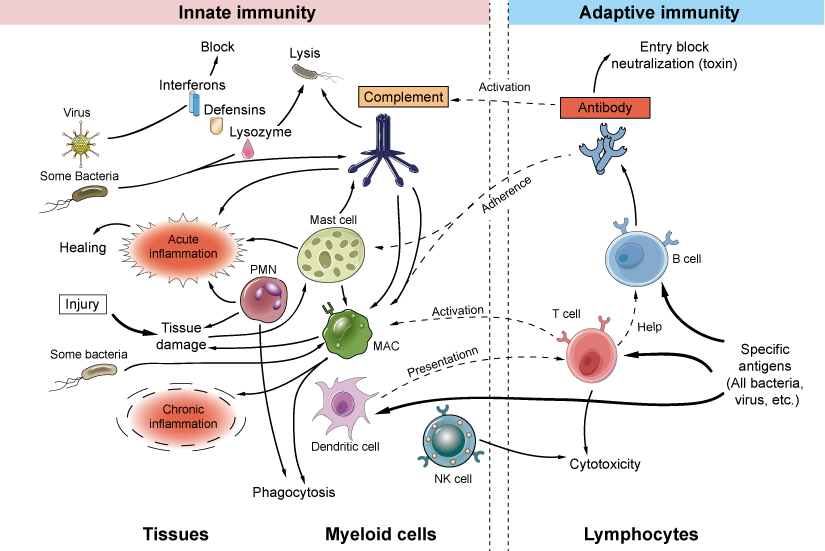
\includegraphics[width=0.9\textwidth]{figures/innate_and_adaptive.png}
    \caption{
        \label{fig:innate_and_adaptive}
        Connection between the innate and adaptive immune system.
        Macrophage (MAC), Polymorphonuclear leucocyte (PMN), Natural killer (NK).
        From \url{http://www.creative-diagnostics.com/innate-and-adaptive-immunity.htm}.
    }
\end{figure}


In summary, we can think of adaptive immunity, in a highly idealized and simplistic way, as going through the following steps:
\begin{itemize}
  \item An antigen presenting cell (e.g.\ a macrophage or dendritic cell) engulfs a foreign protein and presents a its peptide in MHCII.
  \item A T cell clone with TCRs binding this MHCII:peptide complex gets clonally expanded.
  \item A B cell clone binds the same foreign protein, engulfs it and presents its peptides in MHCII.
  \item The clonally expanded T cells bind these MHCII:peptide complexes, inducing B cell proliferation and the production of antibodies.
\end{itemize}
Each item on the list has many details omitted for the sake of simplicity, but one thing missing and worth to highlight is the concept of memory.
The list ends with clearance of the infection through secretion of antibodies binding the pathogen, but this process is slow and very energy consuming, so keeping a memory of the pathogen is an important mechanism to mount rapid response towards repeated infections.
Immune memory is build by immortalizing T and B cells involved in the adaptive immunity reaction of the first encounter with a pathogen, then whenever the same pathogen is encountered again, memory cells will quickly be able to start attacking the invasion.







\subsection{B cell receptors}
The adaptivity of adaptive immunity lies in the diversity of BCRs and TCRs.
Like so many receptors involved in the immune system both BCRs and TCRs are built up by protein domains from the immunoglobulin superfamily.
But unlike other receptors in the immune system they are not encoded by a single gene but by several genes stochastically recombined from multiple loci.
Mechanisms of generation of BCRs and TCRs are so overlapping that it will be sufficient in the following section to only describe the mechanism of generating BCRs.

Antibodies are the secreted form of a BCRs having with the same structure except for the missing membrane anchor.
A BCR is a tetrameric protein of two pairs of identical chains referred to as the heavy and light chains because one is longer than the other, see a) in figure \ref{fig:BCR_structure2}.
The heavy/light chain pairs are linked together covalently by disulfide bonds, likewise are the two heavy chains from each pair, making a BCR a very stable structure.
Both chains starts with a variable region that defines the antigen binding ability of an antibody, and ends with a non-variable constant region (CH1-3/CL).
The number of different variable regions found in a sample of naive (non antigen experienced) human B cells reveal that there are orders of magnitude more different BCRs than single genes on the genome.
Instead of being gene encoded this diversity is introduced by recombining several pieces of DNA from different loci into a full-sized variable region, see b) in figure \ref{fig:BCR_structure2}.
These segments are called the germline genes and for heavy chain sequences there are three groups, the variable (V), the diversifying (D) and the joining (J).
These V, D and J germline gene groups have multiple variants existing in sequential order on the chromosome, and during a stochastic process called VDJ recombination, one of the genes from each germline gene group is physically spliced together into a full-size variable region VDJ gene.
Coupled to a constant region gene further downstream this is being transcribed and translated into one of the heavy/light chains of a BCR protein.

\begin{figure}
    \centering
    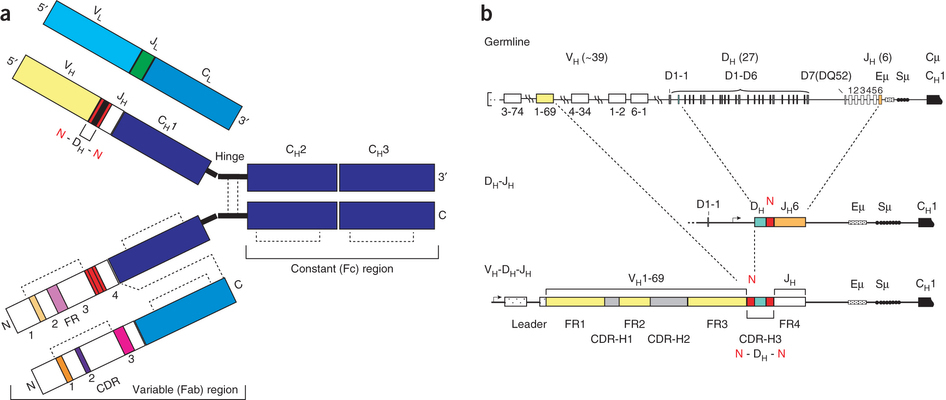
\includegraphics[width=1\textwidth]{figures/ab_structure.jpg}
    \caption{
        \label{fig:BCR_structure2}
        Antibody structure and germline organization on the genome.
        From \cite{georgiou2014promise}.
    }
\end{figure}


While VDJ recombination is not a completely random process \cite{li2012recombinatorial}, it is the basis of all the variability in the variable region in a BCR sequence.
But the combinatorics of all the germline genes are only modest, $\approx 39\times27\times6=6318$ different VDJ combinations times two (due to humans being diploid organisms), vastly less than what is observed in experimental studies.
The rest of the observed diversity comes from another stochastic process involving trimming and inserting new nucleotides at those DNA ends that are joined together, see figure \ref{fig:VDJ_recomb}.
The extra nucleotides added in the junction between V-D and D-J are called N/P nucleotides and the length of these indels can vary from zero to tens of nucleotides.
Although the observed distribution of junctions lengths is not uniformly random, and there is a bias in the inserted nucleotides \cite{murugan2012statistical}, \cite{elhanati2015inferring}, N/P nucleotides adds orders of magnitude more diversity to the combinatorics of gene recombination.
Furthermore all the junctional diversity is contained in the third complementarity defining region (CDR), as opposed to the framework region (FR), see figure \ref{fig:VDJ_recomb}.
As the name suggests the CDR is the structural region that binds the antigen, and to enable binding of a wide range of structures this region must be highly diverse.
Based on a combination of gene recombination and junction diversity and weighted by their distributional biases, Elhanati et al.\ estimated that the naive repertoire is $10^{16} - 10^{18}$ productive sequences \cite{elhanati2015inferring}.
The sequences resulting directly from VDJ recombination and N/P bases are referred to as naive sequences to reflect that these are in a stage before antigen experience and germinal center maturation explained later.
All this diversification occurs within all individuals in the B cell generation in the bone marrow, however with the subtle difference that VDJ genes can differ between individuals.
The different VDJ genes are called alleles and have the potential of expanding the binding breadth of the population wide BCR repertoire even further.

\begin{figure}
    \centering
    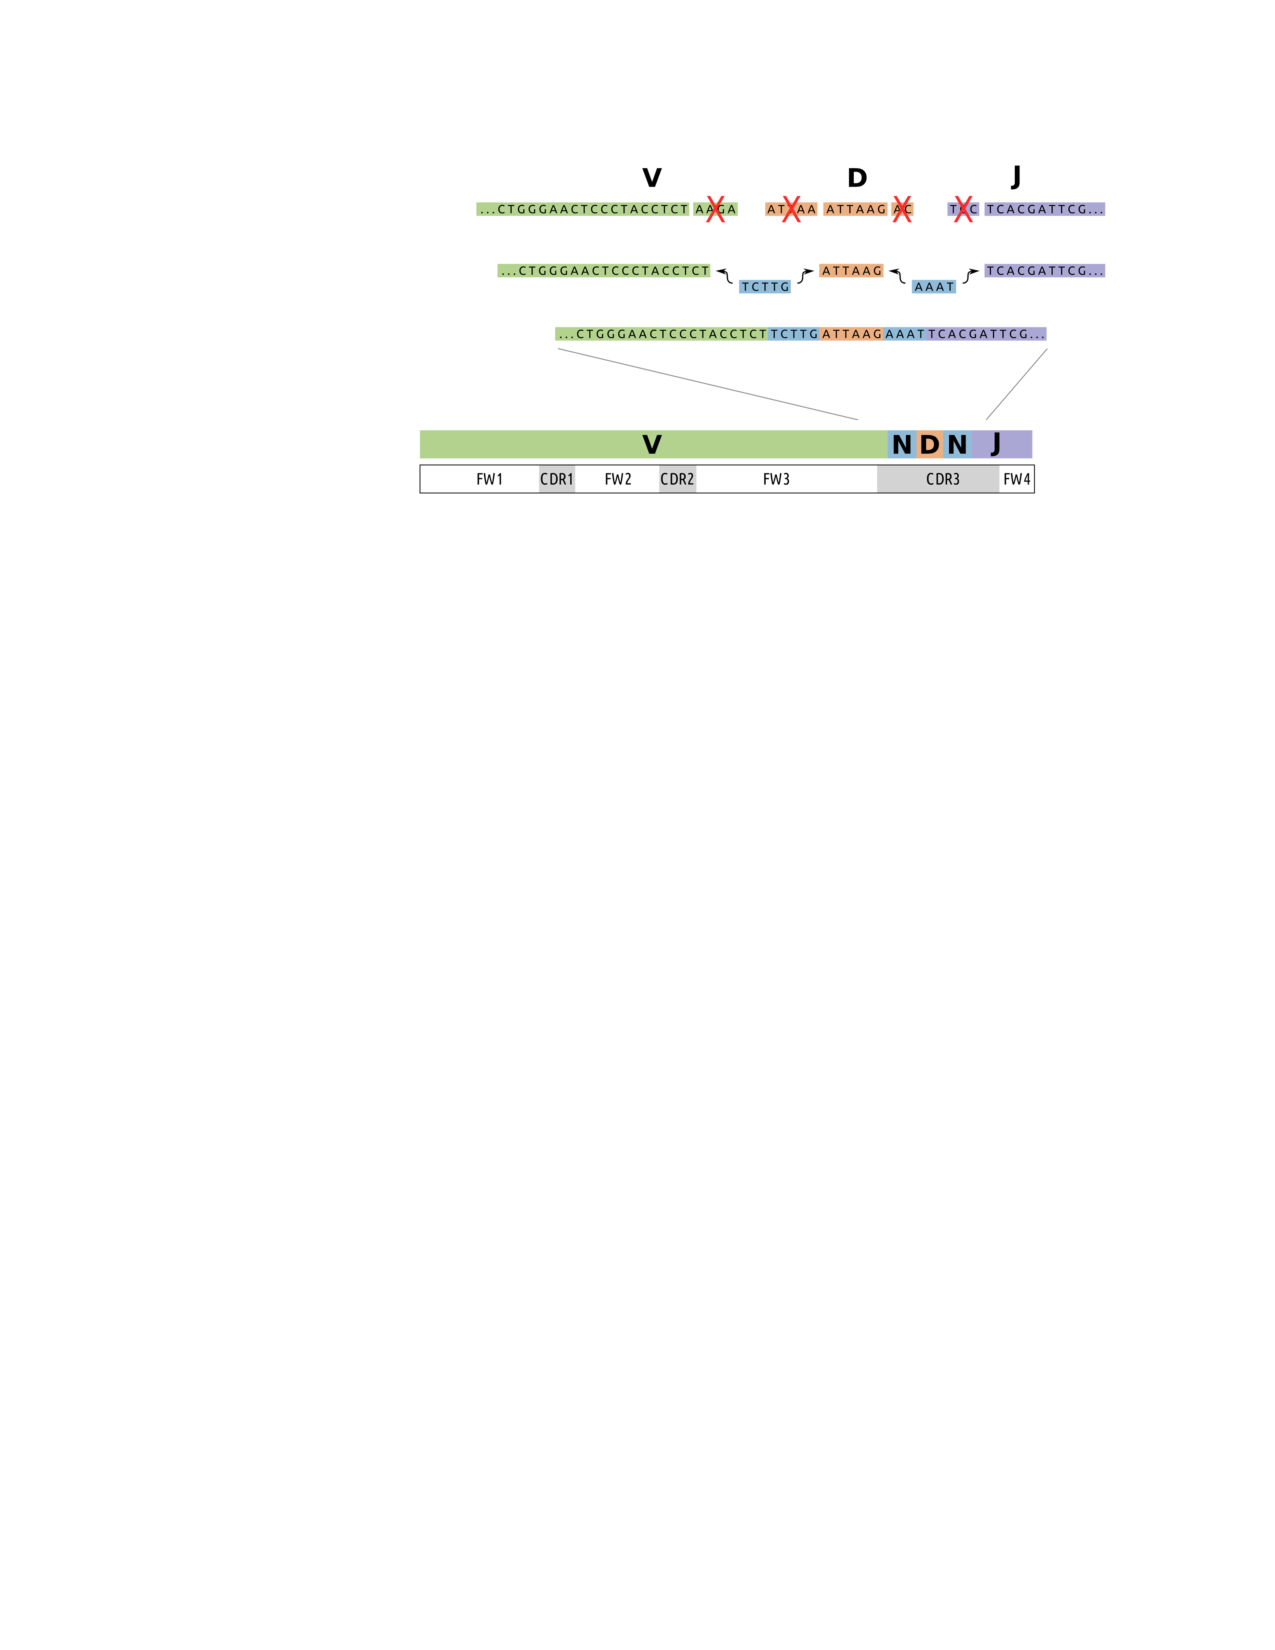
\includegraphics[width=0.7\textwidth]{figures/VDJ_recomb.pdf}
    \caption{
        \label{fig:VDJ_recomb}
        VDJ recombination and introduction of junctional diversity by exonuclease activity and N/P nucleotides added to the joining ends.
        From \cite{ralph2016consistency}.
    }
\end{figure}


While the above description covers the concepts of BCR diversification in general it was applied specifically to an example of a heavy chain variable sequence.
The light chain variable sequence is generated by similar recombination, but light chains do not have the D germline gene and therefore only performs a VJ recombination with substantially less junctional diversity.
Light chain germline genes are present in two non-identical copies named kappa and lambda residing on different chromosomes.
The light chain sequence will only be expressed from one of these, the choice of which is determined by a selection process in the bone marrow excluding self-antigen binding BCRs.
Pairing of a heavy and light chain sequence yields an even larger possible naive repertoire, and with a production rate of at least $10^7$ naive B cells per day \cite{murphy2008immunobiology}, it is not surprising that the adaptive immune system can recognize nearly all foreign antigens.
With such a broad range of antigen binding there will naturally be many BCRs binding endogenous proteins (self-antigens).
This is not desirable because it would lead to immune attach against host cells, known as autoimmunity, and therefore the adaptive immune system has a strict selection process in the bone marrow to destroy B cells with non-functional or self-antigen binding BCRs.
A similar process is happening for T cells in the thymus.




\subsubsection{Germline nomenclature}
The standard nomenclature for BCR genes used throughout this work is defined by the IMGT ontology summarized in figure \ref{fig:IMGT_classification} and described by Lefranc \cite{lefranc2001nomenclature}.
The first part of the gene name is always "IG" and followed by a locus identifier that can be either H (for heavy chain), K or L (for kappa or lambda light chain).
The next letter represents the gene group which can be V, D or J for the variable region, and for the constant region the different isotypes e.g.\ A, E, G1, G2 etc.

\begin{figure}[ht]
    \centering
    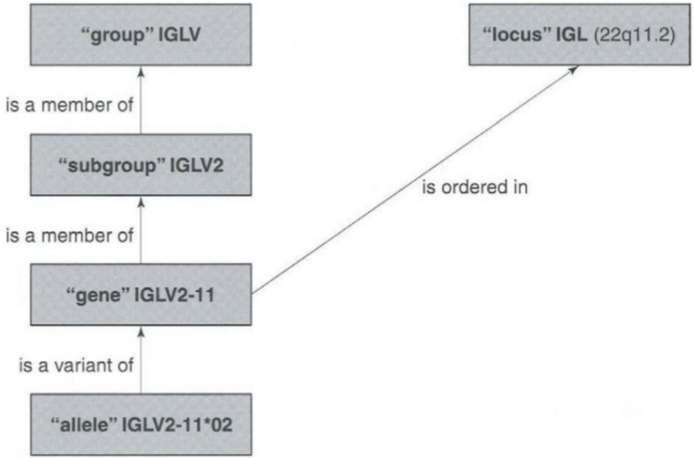
\includegraphics[width=0.6\textwidth]{figures/IMGT_classification.png}
    \caption{
        \label{fig:IMGT_classification}
        IMGT germline gene ontology.
        From \cite{giudicelli1999ontology}.
    }
\end{figure}


For the variable region gene group additional layers of nomenclature are needed since there are many different V, D and J genes under each group.
The first layer is the subgroup level which is defined as a cluster of genes sharing at least 75\% nucleotide similarity.
There are 7 of these subgroups in IMGT and presumably they each derive from distinct gene duplication events, an interpretation supported by the distances separating subgroup genes on their inferred phylogeny, see figure \ref{fig:IGHV_tree}.
However the subgroup level is \textit{not} defined phylogenetically, even though it might coincide with a phylogenetic interpretation.

\begin{figure}
    \centering
    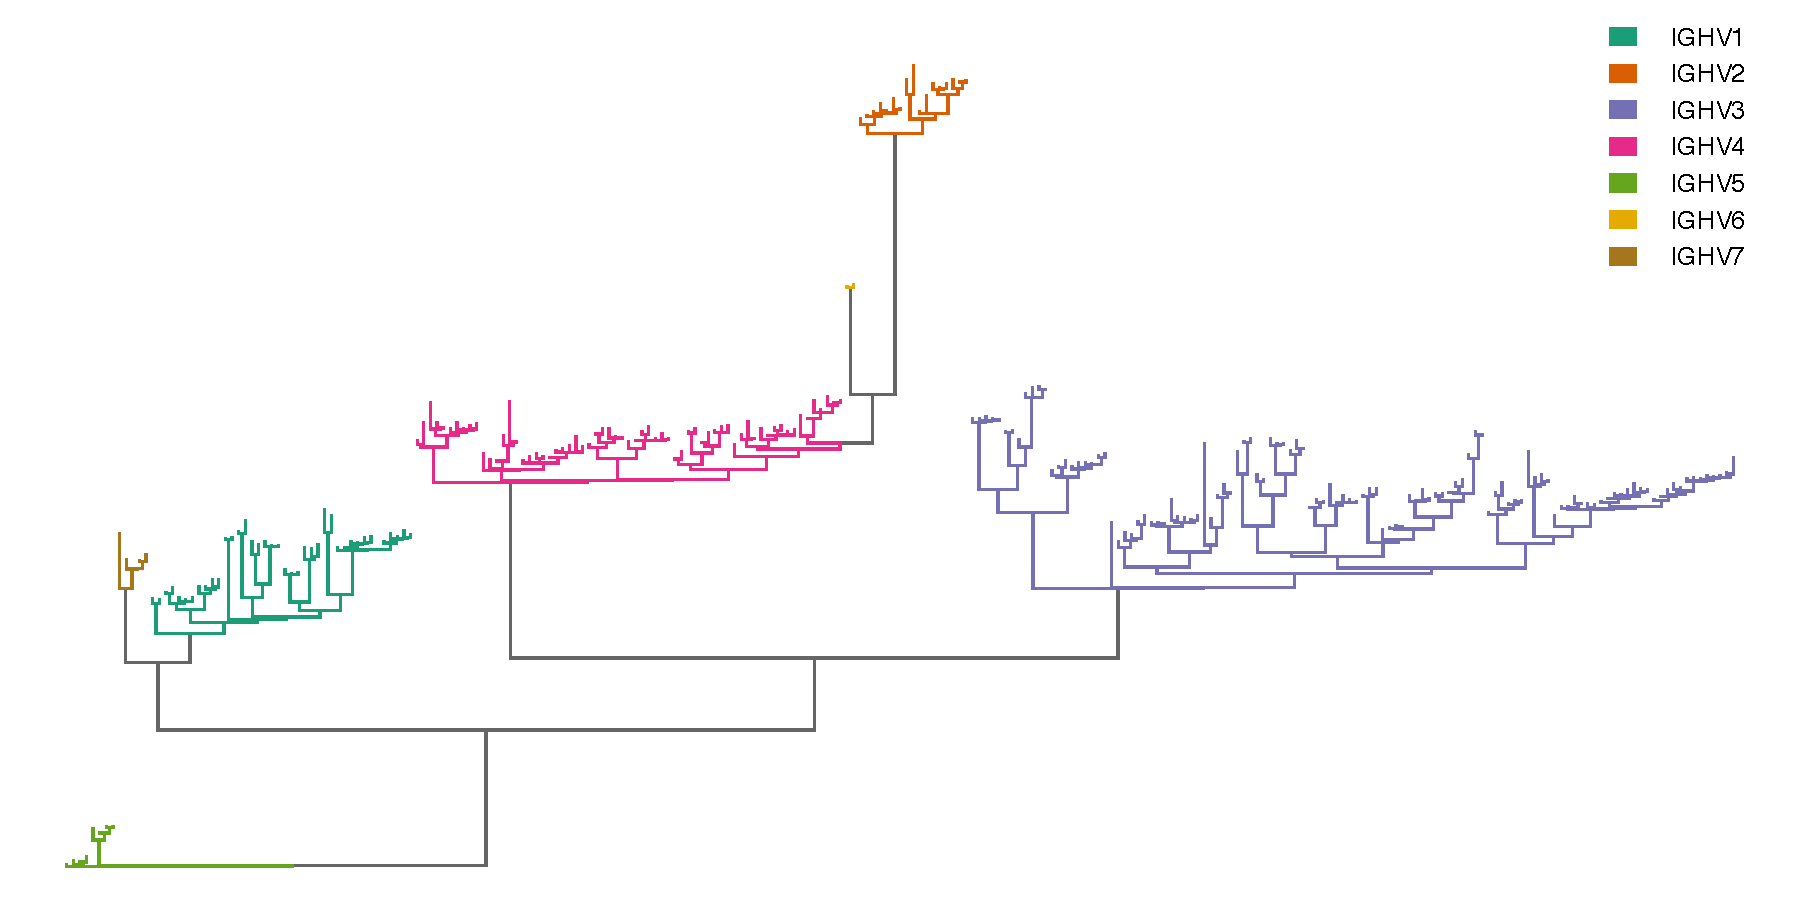
\includegraphics[width=1\textwidth]{figures/tree_right_side_up.pdf}
    \caption{
        \label{fig:IGHV_tree}
        Tree of germline V genes.
        All IGHV alleles were downloaded from IMGT, pseudo genes were removed and a multiple sequence alignment generated with BAli-Phy \cite{suchard2006bali} and MAFFT \cite{katoh2013mafft}.
        BAli-Phy was also used in tree inference, given a fixed topology within each IGHV subgroup determined by RAxML \cite{stamatakis2008rapid}.
        Figure credit: Andy Magee.
    }
\end{figure}


Each subgroup have a number of genes that are defined by their chromosomal position (locus) and present in all individuals in a species.
Each gene is encoded by a single sequence, the allele, that can vary between individuals and will by present in two copies, one on each chromosome copy.
A gene can have many different observed alleles in a population, and while these allelic differences between individuals are usually just single nucleotide polymorphism, indels do occur causing some alleles of the same gene to have different length.

The rules described above are those intended by the IMGT nomenclature derived from regular genetics, however it turns out that gene duplications/deletions are commonly observed at the immunoglobuline locus in both humans \cite{scheepers2015ability} and other animals \cite{collins2015mouse}, \cite{corcoran2016production}, and hence it is not certain that all individuals will have the same number of genes on the same chromosomal locations.
This is a large problem for germline annotation and mutation frequency estimation but as of now it is still an unresolved problem.
However, for a majority of the human data, the germline gene set is comprehensive enough that no major errors are expected, and in this case IMGT nomenclature can be used reliably.
Nonetheless, it is worth to keep in mind that gene duplications/deletions can be a problem, especially with data derived from non-European individuals \cite{scheepers2015ability}.







\subsubsection{Antibody numbering}
For both B and T cell receptors the huge diversity of the variable region is obvious on the sequence level, but much less so on the protein structural level.
Actually even the variable region of a highly mutated BCR is strictly following the structural constraints of a beta-sheet sandwich structure defining the immunoglobulin domain.
Structural conservation also enables a structural consistent mapping from an amino acid sequence onto an antibody protein structure.
A mapping like this was first proposed as a numbering scheme where the immunoglobulin structural components are numbered, and then these numbers are mapped back to the linear amino acid sequence.
First attempt at this was described by Kabat \cite{national1983sequences} and based on a few invariant residues used as anchor points and located by a rule based matching algorithm (these rules are tabulated by Dr.\ Andrew Martins \url{http://www.bioinf.org.uk/abs/}).
Unfortunately this scheme is not good at handling insertion in the flexible CDR regions e.g.\ CDR1 insertions and/or very long CDR3 \cite{martin2010protein}.
Years later came another numbering scheme named after the first author of Clothia et al.\ \cite{chothia1987canonical}.
The Clothia scheme was set out to correct the wrong mapping of CDR1 insertions and thereby achieve structurally consistent mapping, but was first later updated to also accommodate structural consistent mapping of framework indels.

In 2003 the IMGT numbering was proposed as a way to unify numbering of BCRs and TCRs \cite{lefranc2003imgt}.
Similar to the IMGT scheme another scheme, called AHo, also unified numbering of BCRs and TCRs \cite{honegger2001yet}.
Like Clothia, AHo numbering is structurally consistent, but unlike any other scheme it has a fixed standard length of 149 positions with enough space for even very long CDR3 length sequences.
Only in rare cases of germline indels, or an extremely large number of N/P bases, the scheme has to use insertion codes, which are otherwise standard use in all other numbering schemes.
This fixed length sequence numbering makes analysis much more convenient in addition to being easier to interpret e.g.\ all BCR sequences can be encoded by a vector of length 149 and a given position in this vector always correspond to the same position on the protein structure, regardless of sequence.
%Therefore whenever BCR numbering is used throughout with work AHo numbering will be used if nothing else stated.
The software ``ANARCI'' provides a convenient and free open source solution to annotate BCR sequences with AHo numbers \cite{dunbar2016anarci}, (\url{http://opig.stats.ox.ac.uk/webapps/sabdab-sabpred/ANARCI.php}).

With a numbered BCR sequence also comes the rather arbitrary decision of how to define the boundaries between FRs and CDRs.
Clearly FRs are suppose to be more conserved and less structurally flexible while CDRs are suppose to be flexible and highly variable, but putting a boundary between them is a problem that depends on the context in which these annotations are used.
We consider FRs to be the most structurally conserved beta-sheets in the immunoglobulin domain while CDRs are considered to be the structurally flexible loops connecting these beta-sheets.
This definition is recapitulated in the CDR centric numbers tabulated by Andreas Pl{\"u}ckthun (\url{https://www.bioc.uzh.ch/plueckthun/antibody/Numbering/}).
The FR1-4 ranges are: \texttt{1-27, 41-57, 78-108, 138-149} and the CDR1-3 ranges are: \texttt{28-40, 58-77, 109-137}.






\subsection{Biology of the germinal center reaction}
It was discovered by Eisen and Siskind already in 1964 \cite{eisen1964variations} that antibody affinity is steadily increasing during the course of an immune reaction.
The phenomenon is known as affinity maturation and by employing single cell techniques for staining, sorting and sequencing it has now been revealed that maturation is driven by a Darwinian selection process spatially confined into small nodules called germinal centers (GCs) that forms in the lymph nodes.
Affinity maturation typically starts by GC formation 6 days after immunization in begun and ends 4 weeks later when the GCs are dissolved due to B cell apoptosis \cite{victora2012germinal}.
Before dissolving, a GC will export plasma cells that secretes large quantities of high affinity antibodies, but also memory B cells that will work as a permanent memory to be quickly re-initiated upon repeated antigen exposure.

\begin{figure}[!ht]
    \centering
    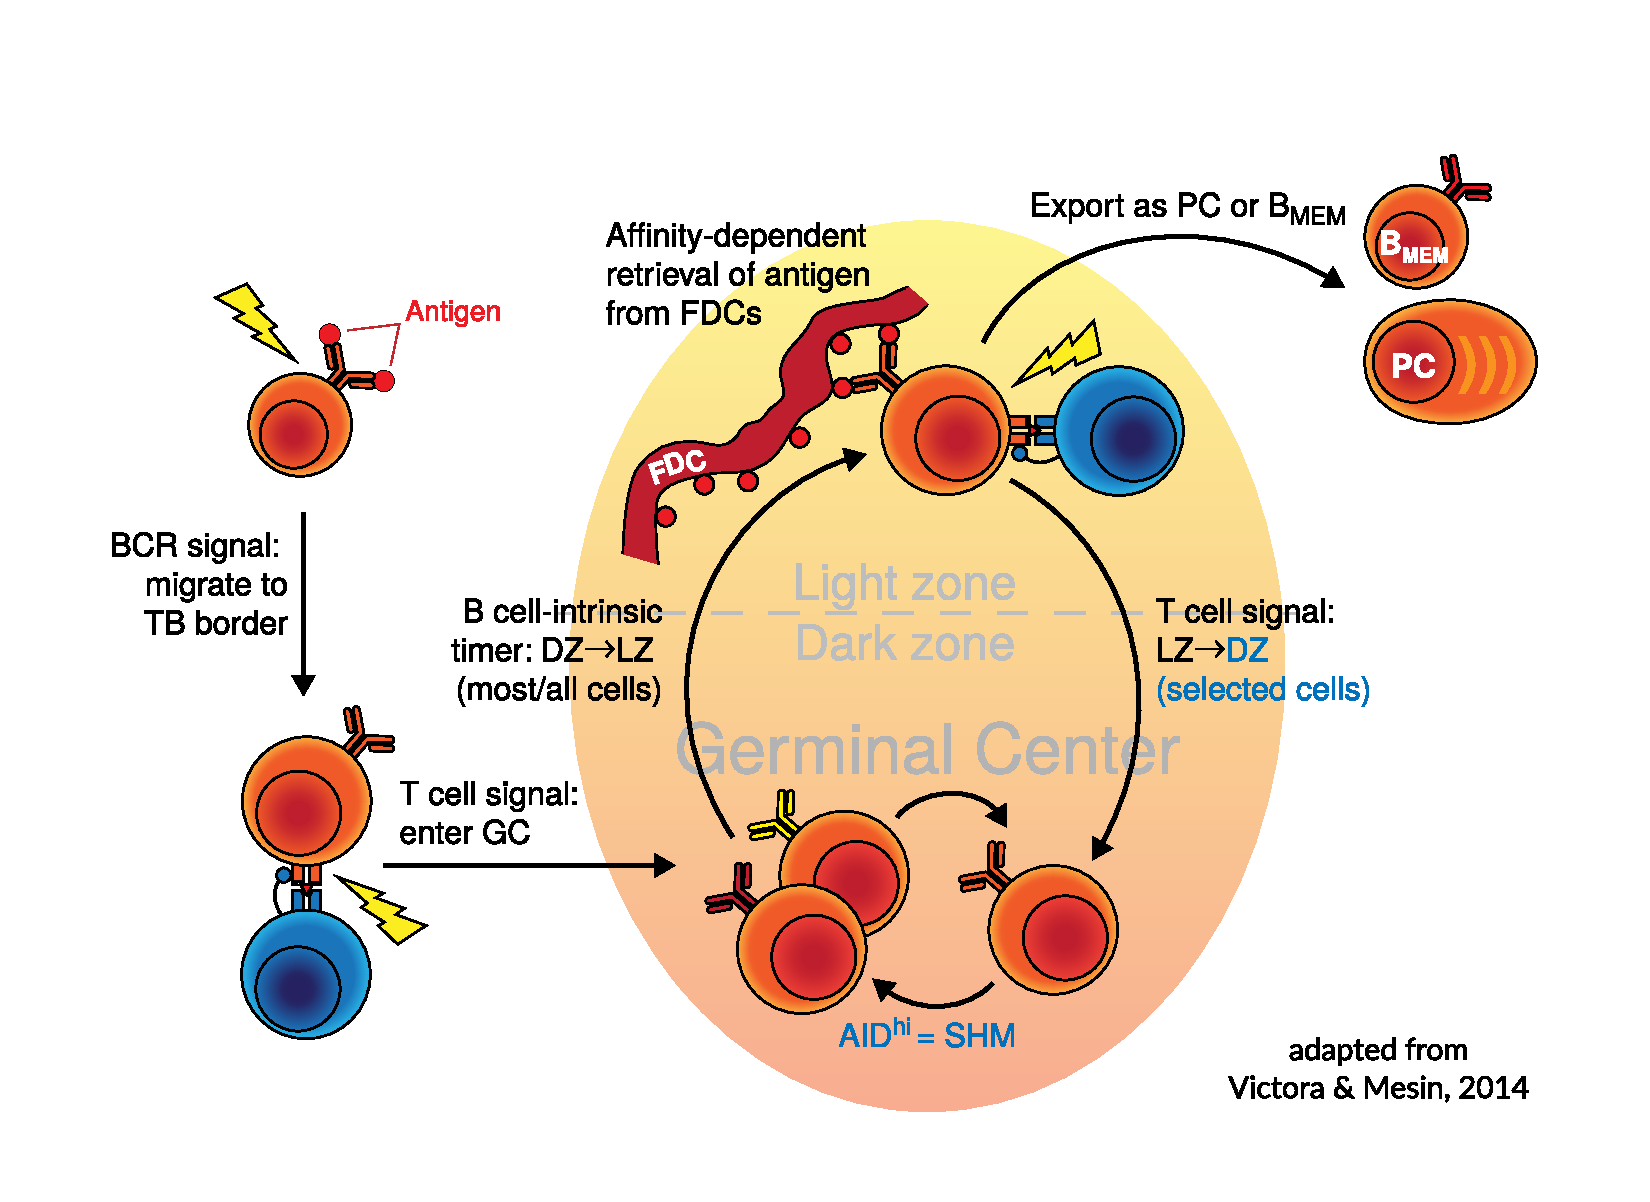
\includegraphics[width=0.6\textwidth]{figures/GC_reaction.pdf}
    \caption{
        \label{fig:GC_reaction}
        Dynamics of the GC reaction, adapted from \cite{victora2014clonal} by Frederick Matsen.
        Follicular dendritic (FDZ) cell in red, T follicular helper (Tfh) cells in blue and B cells in orange.
    }
\end{figure}


Taking a step back, the formation of a GC starts with an immune reaction against an antigen.
Two things are required in the initial phase, a) T cells with TCRs specific for an MHCII:peptide complex presenting a peptide from the antigen and b) B cells with BCRs that can bind the whole antigen, engulf it and present its peptides in MHCII for the T cells to bind, see figure \ref{fig:GC_reaction}.
When these two requirements are fulfilled GC foci will start to form in the lymph nodes.

A GC is a micro-environment containing follicular dendritic cells (FDCs), T follicular helper (Tfh) cells and of course B cells.
The FDCs are antigen storage cells, they capture large amounts of whole proteins and presents them intactly on the cell surface where they can be bound and extracted by B cells.
The B cells undergo a mutation/selection process with two elements a) T cell help and selection and followed by b) mutation and proliferation.
The two elements are spatially separated in the GC and defined as the light zone (LZ) and the dark zone (DZ), called so because the dark zone is more densely populated with cells and appears darker when viewed under a light microscope.
In the LZ B cells are attracted to the large surface of the FDC membrane through its secretion of the chemokine CXCL13, and some B cells will have BCR affinities strong enough that they are able to bind and release antigen from the FDC membrane \cite{suzuki2009visualizing}.
Released antigen will be engulfed, processed and presented by MHCII molecules for Tfh cells to bind.
The more antigen a B cells is sequestering, the more peptide is presented and the more Tfh binding will occur.
If sufficient Tfh binding is achieved the B cell is signaled to migrate to the DZ by following another chemokine CXCL12.
In the DZ it proliferates while expressing high levels of the somatic hypermutation (SHM) inducing enzyme activation-induced cytidine deaminase (AID).
This results in an approximate mutation rate of $10^{-3}$ per position per cell generation ($10^{6}$ higher than the normal rate), and a cell cycle time of only 6-12 hours, introducing a large amount of sequence variability in the DZ cells \cite{victora2012germinal}.
Eventually the progeny cells re-enter the LZ and the SHM induced variability will undergo selection and thereby completing the cycle.
B Cells are constantly cycling between LZ and DZ by switching between high expression of chemokine receptor CXCR5 and low expression of CXCR4 to migrate towards chemokine CXCL13 in the LZ, and low expression of CXCR5 and high expression of CXCR4 to migrate towards CXCL12 in the DZ.
This process is called cyclic re-entry and it continues until the GC dissolves through a mechanism still unknown.
During selection there are a limited amount of Tfh cells, so this is where B cells have to compete to get the activation signal.
The more antigen a B cell can sequester relative to the others, the more likely it is to get Tfh help, migrate to the DZ and go on to proliferate, as oppose to undergoing apoptosis if Tfh help is insufficient.
By an unknown mechanism a fraction of the B cells in the LZ will get a special Tfh differentiation signal and these are exported outside of the GC with fate as either a plasma cell or a memory cell.

While many mechanistic details of the GC reaction is known much remains to be elucidated.
The mechanisms of selection has been difficult to study, but current evidence suggests that it is solely mediated through T cell interaction \cite{victora2012germinal}, \cite{victora2014clonal}.
Although the importance of Tfh interaction has recently been challenged \cite{yeh2017limit}, it currently remains as the best model for understanding the observations all the mechanisms of selection.
Selection can be split into three main elements:
\begin{itemize}
  \item Affinity
  \item Stability and expression
  \item Self-antigen binding
\end{itemize}

To improve antigen affinity is the most obvious point for selection to occur on.
A gain in BCR affinity will enable a B cell to sequester more antigen from the FDCs and present more MHCII:peptide to the limited number of Tfh cells.
Those B cells that have many MHCII:peptide complexes are much more likely to interact sufficiently to get the signal for proliferation, meaning that higher affinity is positively selected.
An extension to this is in the case of mutations altering the stability and/or expression of a BCR, resulting in less BCRs to be presented on the cell surface.
Lower BCR levels on the cell surface will cause less antigen sequestering from the FDCs resulting in less Tfh cell interaction leading to negative selection.
Finally a more convoluted example of Tfh cell mediated selection is the negative selection of self-antigen binding BCRs.
%It has been suggested that self antigen binding B cells will mostly present self antigen derived peptides in MHCII because of the large quantities of self antigen compared to the immunizing antigen \cite{Sabouri_2014}, \cite{Bannard_Cyster_2017}.
Self-antigen binding B cells are simply clogging up MHCII molecules with self-peptides leading to less T cell help \cite{Sabouri_2014}, \cite{Bannard_Cyster_2017} and negative selection.
Again, this mechanism is conveniently explained by a Tfh cell mediated selection process.

Despite the convincing mechanistic understanding it must be stressed that the GC reaction contains many, either mechanistically unknown, or purely stochastic elements.
E.g.\ even though there is an observed relationship between clonal bursts and mutational induced gain in affinity, this does not appear to happen consistently i.e.\ large affinity gains are observed without clonal bursting \cite{tas2016visualizing}, supporting the conclusion that either selection is highly stochastic or other mechanisms are still unknown or unmonitored e.g.\ higher affinity but worse expression could make the net balance of selection turn negative, while it appears to be positive if only looking at affinity.

A notable case of a correction to the mechanistic understanding of the GC reaction happened recently.
In 2012 a review by Victora, based on all previous evidence, suggested that GCs are initially colonized by little as 1-3 naive B cells \cite{victora2012germinal}.
However, just 4 years later the same author concluded in Tas et al.\ \cite{tas2016visualizing} that this number was largely underestimated.
Using an elegant experimental setup, they were able to visualize the colonization of GCs in multiple lymph nodes across different mice and concludes that mice GCs are consistently being colonized by 50-200 naive B cells.
Before the Tas et al.\ paper in 2016 it had been a good approximation to assume that GCs were being founded by just a single cell, and that this monoclonality would be upheld throughout the entire GC reaction.
In the view of monoclonality the GC identity has been a convenient definition of a B cell clone, but this view has to be redefined with the findings that GCs are starting out as highly polyclonal, and even ends up with a substantial fraction of GCs that keeps being polyclonal throughput the whole GC reaction.
Complicating things further, Tas et al.\ also observed that B cells with the same naive sequences were found across multiple GCs reacting to the same antigen.
For an updated definition it would be fair not to distinguish between B cells with identical naive sequences but matured in different GCs, as long as they mature against the same antigen, because then they are under the same selection pressure.
But then two distinct clones would need to be defined if two B cells with the same naive sequence were independently matured towards different antigens.
However it is a) practically very difficult to distinguish clones that have identical naive sequence and b) very unlikely that the exactly same naive BCR nucleotide sequence will mature towards more than a single antigen.
Therefore the old and impractical definition of a B cell clone is discouraged, and instead the simpler definition from Ralph et al.\ \cite{ralph2016likelihood} is used throughout this work.
In this scheme if two different BCRs are derived from an identical naive DNA sequence, they are in the same clonal family regardless of the GC context they came from.

SHM is driven by the enzyme AID that works by deaminating cytosines during DNA transcription.
DNA repair enzymes are then recruited to the deaminated cytosines, where they with some probability will introduce point mutations both at the site of deamination or at neighboring sites.
Increased mutation rate during SHM is therefore the combined effects of AID and a number of DNA repair enzymes.
With a whopping $10^6$ times increase in mutation rate during SHM (from $10^{-9}$ to $10^{-3}$ mutations per bp per cell generation), there is a need to contain SHM so it does not run loose and destroys the function of the cell itself.
SHM achieves this by acting preferentially close to the chromosomal location of the variable region genes \cite{Yeap_2015}, \cite{liu2008two}.
In addition SHM appears to be biased and preferentially introduce mutations in some contexts rather than others \cite{Yeap_2015}, incidentally consisting of sequence motifs that are over represented in the variable chain genes.
The contextual bias of AID was initially described as hot/cold spots defined by a few specific 3-mer motifs (WRC/GYW hotspots and SYG/GRS coldspots) observed to change mutation rate significantly by preferentially recruiting AID \cite{pham2003processive}.

It can be difficult to tease apart the different biases introduced by both AID and the DNA repair enzymes, and though the majority of the observed SHM bias most likely comes from preferential AID activity \cite{Pham_2016}, it is their combined effect that is observed as SHM during affinity maturation.
Instead of a mechanistic model of SHM an empirical context model can be setup purely based on a large number of observed mutations and their surrounding nucleotide context.
Such a model has been described by Yaari et al.\ \cite{yaari2013models}, and later in an improved version \cite{cui2016model}, as the so called S5F model.
The S5F model is simply the a list of relative probabilities of observing the middle base mutating in all the possible 1024 5-mer DNA motifs.
Given a motif and a mutation on its middle base, the S5F model also provides the probability of the nucleotide identity of the resulting mutation.
This motif model is completely empirical and relies on the input data which is a large number of BCR sequences that have undergone SHM without selection.
A survival model \cite{cox1992regression} is a good way to describe the observed data, with the event rate Theta, being proportional to the logarithm of the mutation rate of the motif (unpublished data from David Shaw and Jean Feng), see figure \ref{fig:SAMM_plot}.
Fitting the model is non-trivial because neighboring motifs share the same context and in the case of an observed event in one motif this changed the context, and thereby Theta, in the other motifs.

\begin{figure}[!ht]
    \centering
    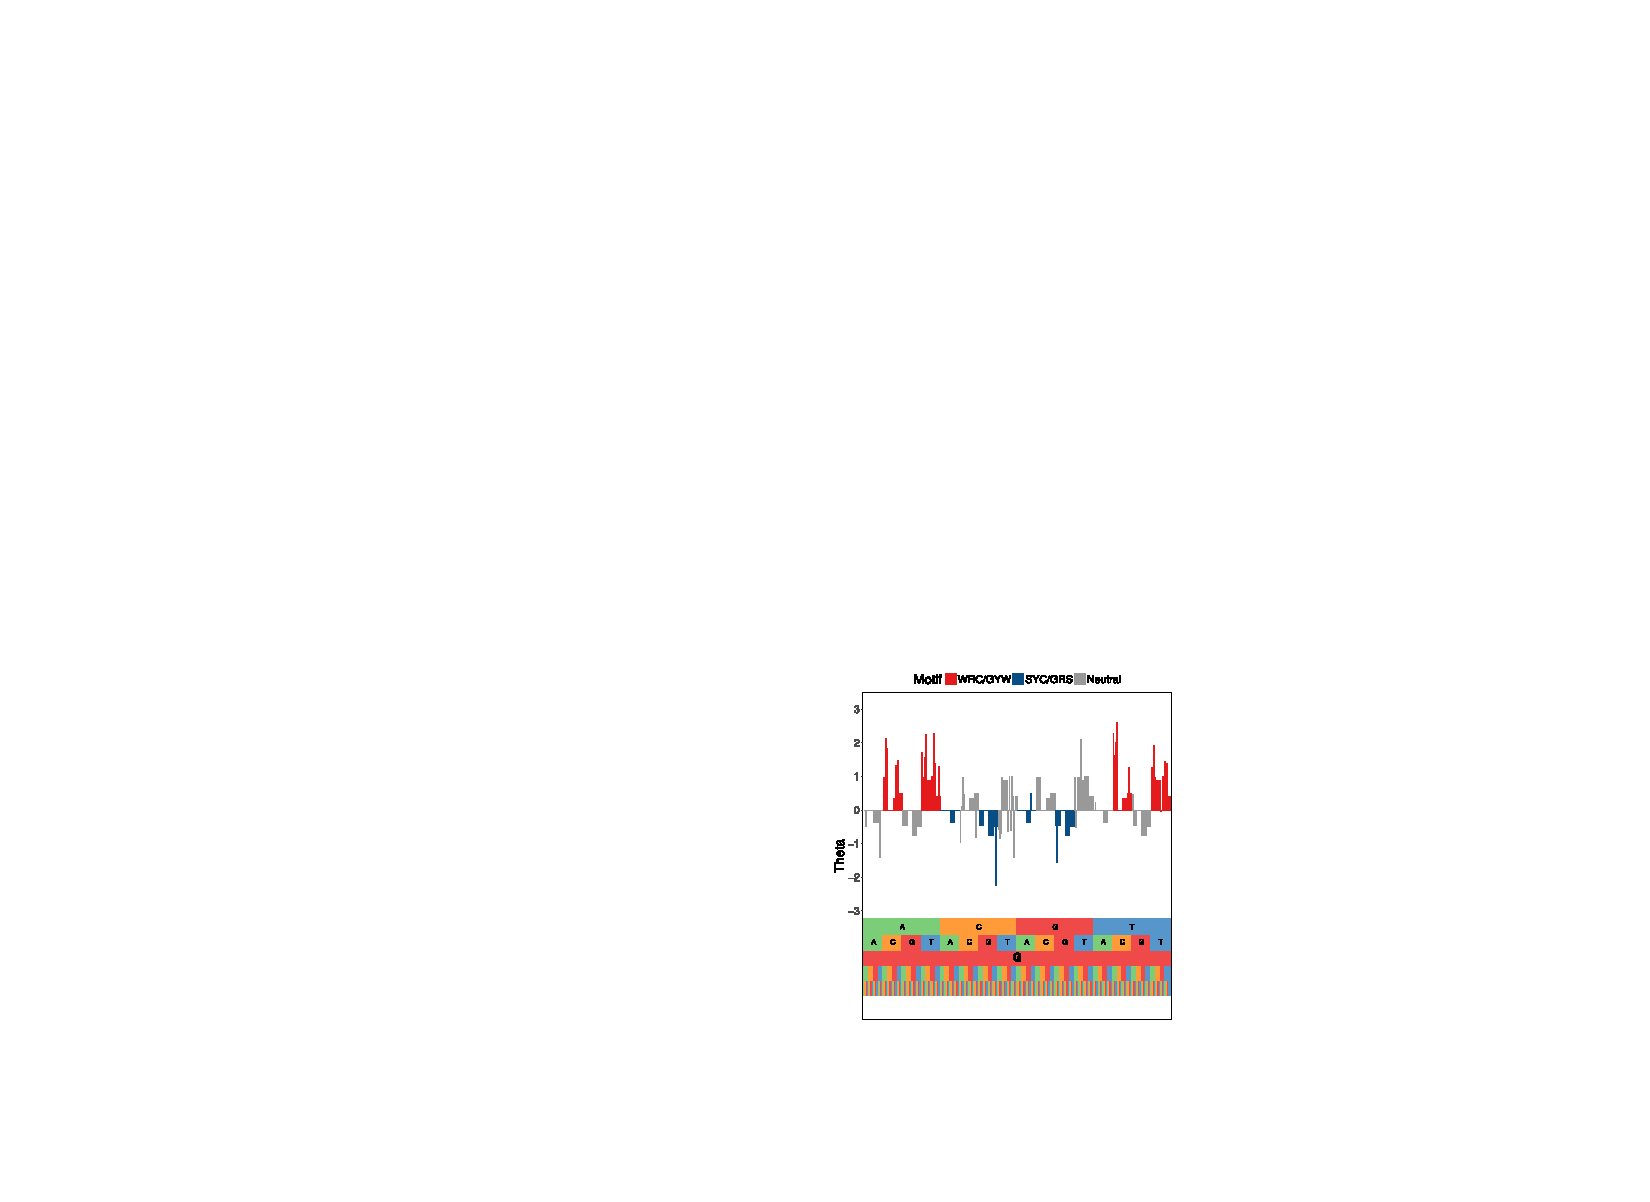
\includegraphics[width=0.45\textwidth]{figures/SAMM_plot.pdf}
    \caption{
        \label{fig:SAMM_plot}
        Plot of a 5-mer SHM motif model analogous to S5F \cite{cui2016model}. Bottom row is the 5'-end of the 5-mer motif progressing upwards to the 3'-end and with G as the central base. Theta is the rate parameter of the survival model and is proportional to the logarithm of the mutation rate.
        Figure credit: David Shaw and Jean Feng.
    }
\end{figure}










\section{Monitoring adaptive immune responses}
During the centuries of immunological research a large array of techniques have been directly invented or adapted from other fields of science to monitor the cells in an immune response.
Starting with hybridoma techniques \cite{larrick1989polymemse}, antibodies could be produced and tested in a single cell setting after which sequencing would reveal the DNA encoding the antibody.
A large number of other techniques was already used or followed e.g.\ ELISA, single cell staining and sorting, ELISPOT, fluorescence imaging techniques etc.
Already in 1991, when Sanger sequencing was the most high throughput sequencing method, the diversity of the immunoglobulin genes and the matured BCR was being explored by sequencing single clones \cite{yamada1991preferential}.
In more recent time sequencing by Illumina and Roche 454 have revolutionized the way we are monitoring adaptive immunity by enabling complete sequencing of millions of different BCR sequences.


\subsection{Repertoire sequencing}
In the following the focus will be on BCR sequencing but the same considerations apply to TCR sequencing.
Several sequencing strategies have been devised to capture various aspects of the immunoglobulin genes, but most start at the same place; the BCR transcripts.
The use of genomic DNA is also possible, but with only a single copy of a highly variable gene, this is prone to failure.
Maybe more importantly, the transcript levels can also be useful information that genome level sequencing cannot provide and therefore most studies do bulk mRNA isolation from tissue or cells of interest, followed by reverse transcriptase PCR (RT-PCR) to create a pool of DNA with PCR primed ends, see figure \ref{fig:BCR_RTPCR}.

\begin{figure}[ht]
    \centering
    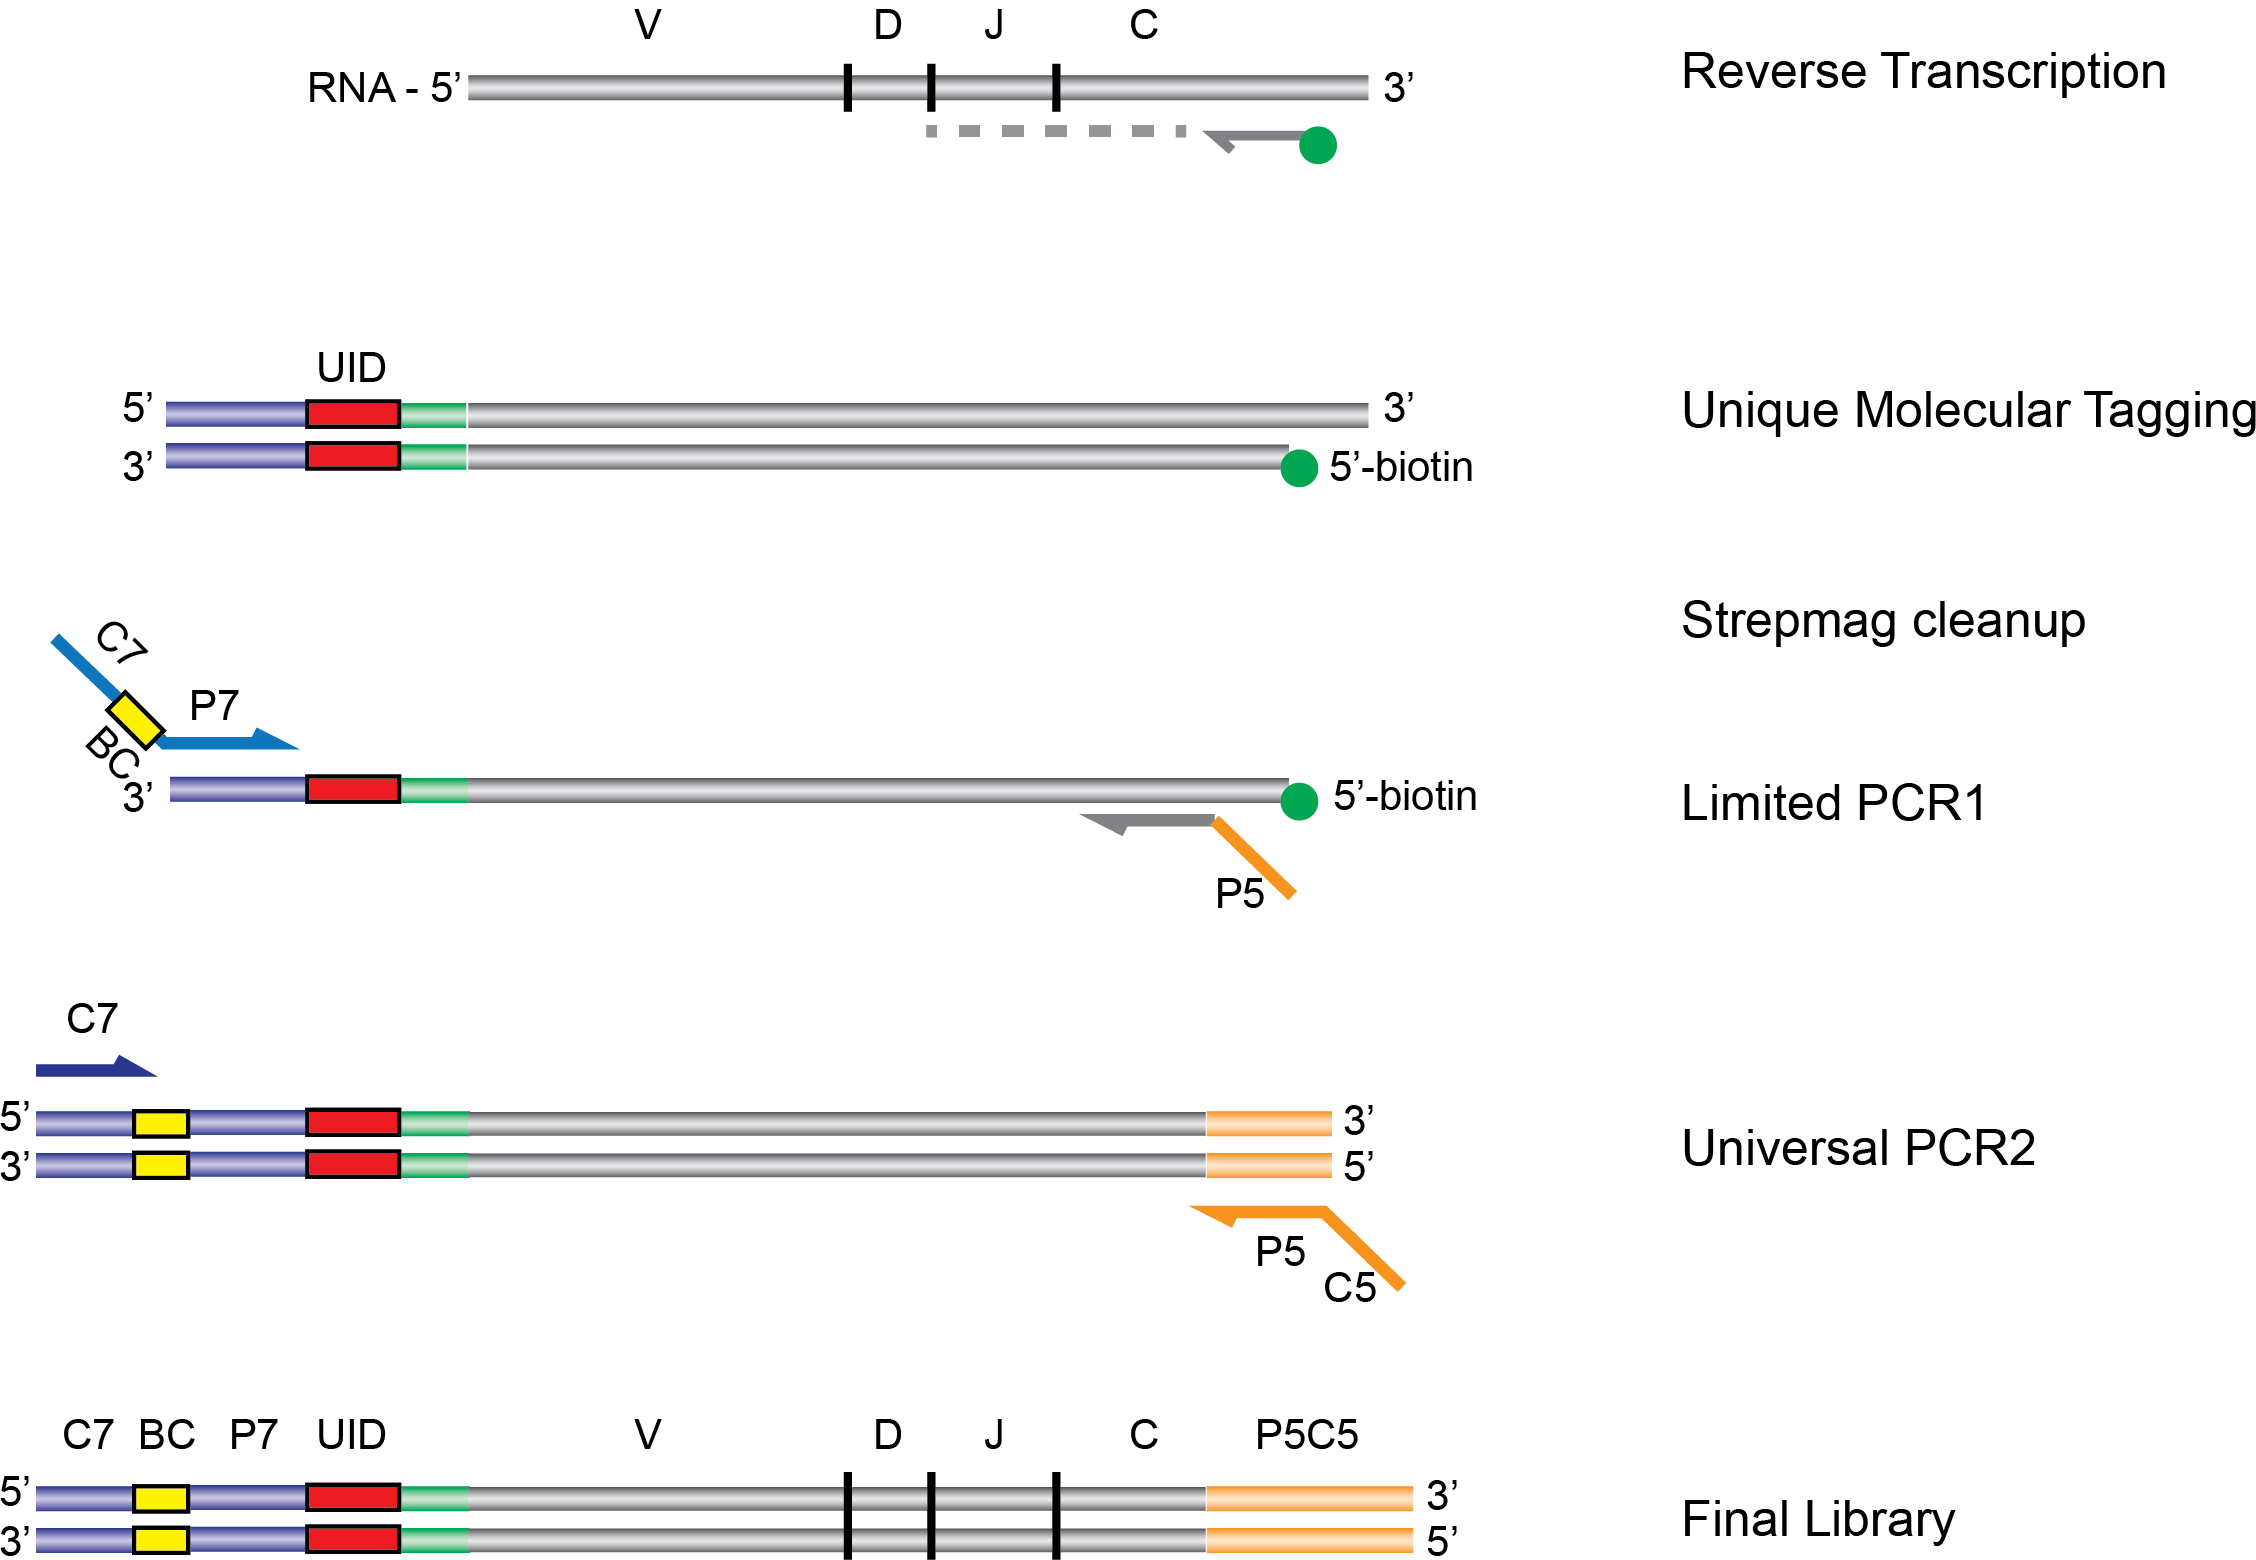
\includegraphics[width=0.8\textwidth]{figures/BCR_RTPCR_AbVitro.png}
    \caption{
        \label{fig:BCR_RTPCR}
        DNA prep method for BCR sequencing on Illumina developed and used by AbVitro (now Juno Therapeutics).
        In the first step an RT-PCR is run with template switching to introduce a UID.
        The fragments are then purified and the Illumina C7 clustering sequence, and barcode (BC), are attached to the 5'-end.
        Finally the C5 clustering sequence is attached and the library is ready for Illumina paired-end sequencing.
        A similar (but not identical) DNA prep method was used in Stern et al.\ \cite{stern2014b} with figure \ref{fig:UMIread} showing the resulting data format.
        Figure from Laustsen et al.\ \cite{laustsen2017exploration}.
    }
\end{figure}

An effective way to minimize errors introduced by the several steps of RT-PCR, PCR and sequencing is to attach a short unique molecular barcode (UMI, also known as unique identifier or UID) to the end of each read already at the RT-PCR step \cite{turchaninova2016high}.
With enough random UMIs in the pool chances are extremely low that the same UMI will be incorporated into multiple BCR transcripts.
Therefore each UMI will represent a single BCR transcript from the unamplified pool of mRNA, and reads with the same UMI should therefore be identical in the rest of the read.
Conversely reads with different UMIs can have identical BCR sequences because a single cell can, and likely will, have multiple copies of the same BCR transcript.
UMIs therefore also provide a way of transcript level quantification on top of its error correction.

Once the read library has been prepared sequencing is undertakes, usually either on Roche 454, or Illumina MiSeq.
In the early days of Rep-Seq the advantage of Roche 454 was its long read length that could be adjusted to span the entire V gene, and additionally going all the way into J when a short CDR3 appeared.
However with the development of the 2x300bp Illumina MiSeq paired-end reads, see figure \ref{fig:UMIread}, the 454 is out phased in favor of higher throughout and better read quality with much lower chance of indel calling.

\begin{figure}
    \centering
    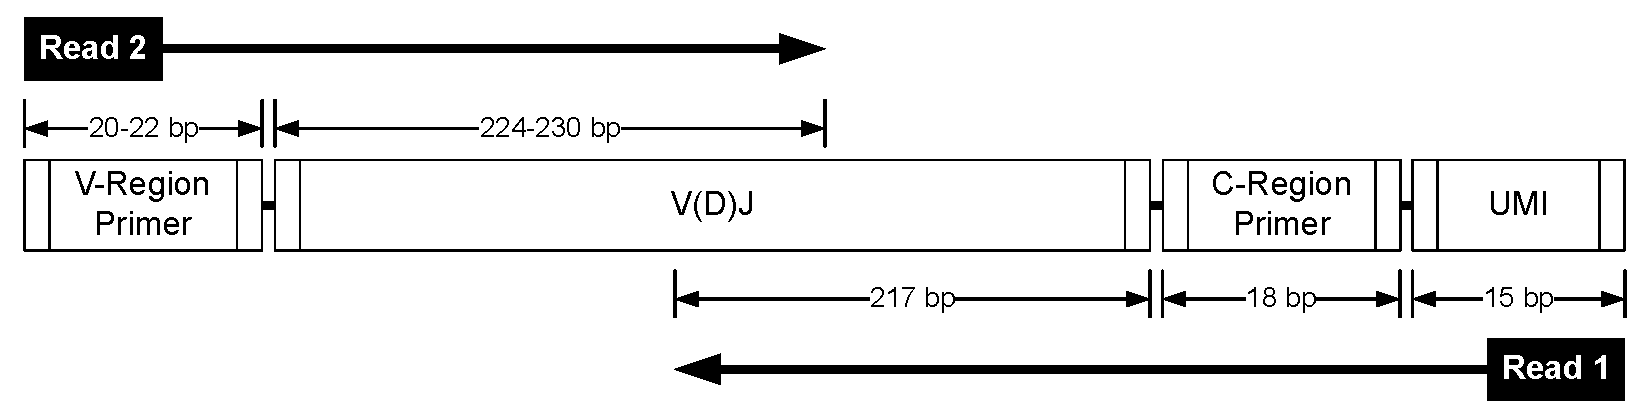
\includegraphics[width=1\textwidth]{figures/Stern2014_ReadConfiguration.pdf}
    \caption{
        \label{fig:UMIread}
        Example of a sequencing strategy for sequencing the full variable BCR chain and parts of the constant region. The strategy is designed for Illumina paired-end reads and seen used in Stern et al.\ \cite{stern2014b}. Figure from pRESTO readthedocs \cite{vander2014presto}.
    }
\end{figure}

After DNA reads have acquired from sequencing, error correction becomes a substantial issue.
In the normal uses of high throughput sequencing, errors are just averaged out by the use of consensus sequences, but in the case of BCR sequencing the inherent variability of the BCR makes it difficult to tease apart what DNA variations that can be attributed to SHM and junctional diversity, and which can be attributed to PCR and sequencing errors.
With the many different sequencing protocols there can also be large differences in the data processing afterwards, but pipelines exists that are fairly generic and will handle a wide range of data.
A commonly used pipeline capable of processing a wide range of data is pRESTO (\url{presto.readthedocs.io}) \cite{vander2014presto}.
Data processing with pRESTO is still sequencing protocol dependent but largely flexible and funnels down the data into the same end point regardless of protocol.
In the case of paired-end Illumina reads with UMIs, similar to figure \ref{fig:UMIread}, the workflow can be summarized by the flowchart in figure \ref{fig:UMIread_flow}.
Input data is paired-end reads with Phred quality scores in fastq format.
The data quality is first assessed by running FastQC \cite{andrews2010fastqc}, then bad reads are removed or ends are trimmed to sufficient minimum quality.
Many DNA prep protocols are using degenerate primers for PCR amplification by binding to the 5'-end of all possible V genes, see figure \ref{fig:UMIread}.
This will possibly introduce what will look like a mutation, but in fact is a PCR artifact due to promiscuous primer binding.
These should be removed by trimming off the primer binding region or "masking" it by reverting these mutations back to germline (red in figure \ref{fig:UMIread_flow}).
Then the paired-end sequences are merged by merging on the overlapping stretch of read 1 and 2 using simple alignment score maximization.
Read pairs that failed to merge are discarded but the reads are still kept in separate files to build a consensus sequence over the sequences with the same UMI.
Then anther instance of pairing is done on these consensus sequences to synchronize the files followed by merging reads into the same file (orange and green in figure \ref{fig:UMIread_flow}).
Next a series of filtering and deduplication steps are undertaken e.g.\ only allowing sequences with multiple reads, a maximum number of ambiguous nucleotides etc. to pass through.
The final result should be a set of high confidence BCR sequences, and depending on the sequencing protocol, with or without information about the constant region and/or mRNA abundances.

\begin{figure}[ht]
    \centering
    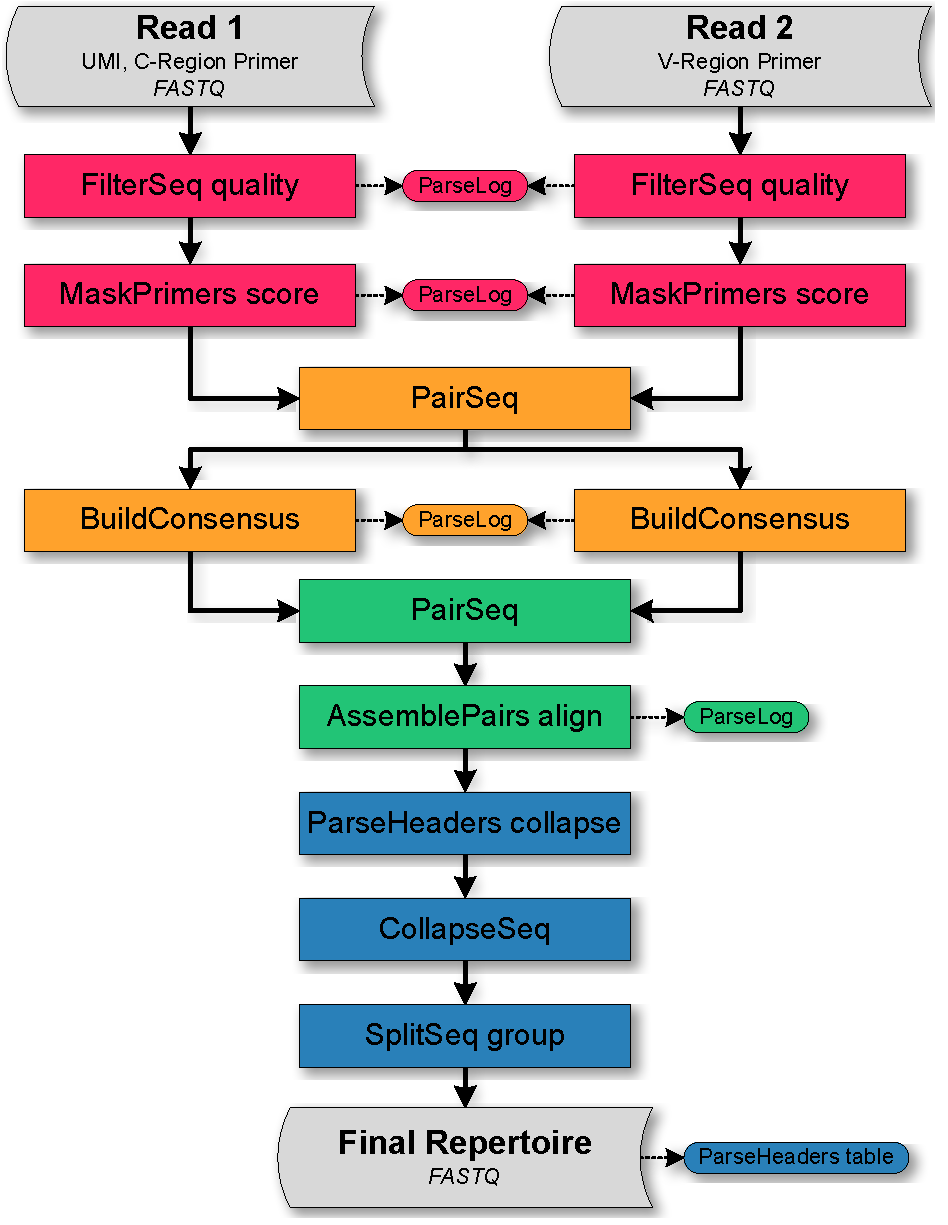
\includegraphics[width=0.55\textwidth]{figures/Stern2014_Flowchart.pdf}
    \caption{
        \label{fig:UMIread_flow}
        Flow of the raw sequencing data through the pRESTO pipeline. This strategy is designed for Illumina paired-end reads, e.g.\ \ref{fig:UMIread}, and seen used in Stern et al.\ \cite{stern2014b}. From pRESTO readthedocs \cite{vander2014presto}.
    }
\end{figure}


All of the above described sequencing methods suffer under the substantial caveat that they are mixing the heavy and light chain sequences from multiple cells under the mRNA isolation step.
This means that a given heavy chain sequence could have been paired with any of the light chain sequences observed for the same sample - and with high throughout sequencing this is millions.
Pairing is not always necessary e.g.\ in some cases of diagnostics, but if the function of an antibody is to be tested the correctly paired heavy/light chain needs to be found.
Some authors have done so using random pairing and selecting for binding via phage display \cite{glanville2009precise}, others have ranked heavy and light chains according to their frequencies from sequencing and matched the highest frequency clones \cite{reddy2010monoclonal}, yet others have used phylogenetics to infer trees and then pair similar topology heavy/light chain trees, guided by a known pair to link to trees \cite{Zhu_undated-zz}, \cite{kwong2017antibodyomics}, \cite{huang2016identification}.
The latest development is to use micro-droplets to capture single cells and then perform the DNA prepping steps inside these drops.
Some authors are pairing heavy/light by physically linking them together via overlap PCR \cite{mcdaniel2016ultra}, while others are amplifying a UMI inside the drop and attaching it to both heavy and light chains \cite{Briggs134841}.
Though the methods for paired heavy/light chain sequencing now exists they are not widely used because of the requirement of having a micro-droplet platform and expert knowledge which is not common stock for most labs.
Still the vast majority of public BCR sequencing data is unpaired and it will likely remain so for at least some years to come.



\subsection{Inferring B cell clonal families}
Once high quality sequences have been obtained from a BCR repertoire sequencing they become the input to the following analysis steps, either as hypothesis testing or hypothesis creating.
A first step in the analysis is simply to annotate sequences by their germline VDJ genes, which can be done simply by aligning each sequence from a database of germline genes to the BCR sequence at hand.
The V, D and J genes achieving the highest alignment score are the winners and inferred to be the true germline gene present on the ancestral naive sequence.
This approach is used by many studies to VDJ annotate BCR sequences, usually either through the NCBI hosted IgBLAST \cite{ye2013igblast} or IMGT's V-QUEST \cite{li2013imgt}.
The advantage of using IgBLAST is its fast turnover and stand-alone software under a permissive license.
Next, an extension to inferring the germline genes is to infer the full naive VDJ sequence of its unmutated ancestor.
Inferring the full naive sequence is a bit more complicated because it requires inferring the original sequence flanking the D gene, where the junctional diversity from N/P nucleotides is complicating the problem.
Given a BCR sequence and assuming some distribution of N/P nucleotide insertion, how many bases is trimmed of the V-D junction and how many are trimmed of the D-J junction?
%Assuming uniform randomly inserted N/P nucleotides nothing can be inferred other than the 25\% chance of either of the bases, however the problem is how many bases is trimmed of the V-D junction and how many are trimmed of the D-J junction?
This question is non-trivial because of SHM e.g.\ if a single mismatch is preventing a V gene alignment match to extend further 4 bases downstream, see table \ref{extend_or_not}, should that be regarded as a mutation due to SHM, or is it regarded as the last 3 random N/P nucleotides incidentally had the same identity (uniform random chances $0.25^3=0.0156$)?
Clearly it looks like an extension to the alignment would be the optimal solution but what then if the last base was also a mismatch? Or that about the effect of the underlying distribution of N/P nucleotide insertions?
In these complex cases intuition starts breaking down, instead there is need for a statistical model that can integrate over probabilities and give consistent estimates.
\begin{table}[ht]
\centering
\begin{tabular}{l}
\texttt{V gene \ ...GTTGAGTGT} \\
\texttt{\ \ \ \ \ \ \ \ ...|||||*|||} \\
\texttt{BCR seq ...GTTGAATGT}
\end{tabular}
\caption{To extend, or not to extend, that is the question (for an HMM to answer).}
\label{extend_or_not}
\end{table}

The classical "go to" statistical model for biological sequence analysis is a hidden Markov model (HMM) \cite{durbin1998biological}.
Briefly an HMM is set of user defined states, e.g.\ the V, D or J genes, N/P insertions, etc., and the jump between states are then connected by probabilities.
Each state has a list of emission probabilities that defines the probabilities of observing a given base.
%There is also a probability of changing state e.g.\ from V gene to N/P insertion.
The hidden/unknown part is the identity of the states at a given position in a sequence e.g.\ when is the V gene stopping and the N/P insertion starting, like the example above.
This is one of the question that is possible to answer using an HMM, specifically by calculating the so called Viterbi path, but what is more interesting is the inherent flexibility of an HMM to represent well known biological mechanisms in a statistical framework.
% It is out of the scope of this work to explain the inner workings of HMMs, how to find the optimal path, estimating parameters etc.
% For this the book by Durbin et al.\ \cite{durbin1998biological} is an excellent resource.

To address the problem of BCR sequence annotation Ralph et al.\ developed an HMM model of VDJ recombination and built it into a software called partis \cite{ralph2016consistency}.
Using extensive simulation studies, the authors observed clear shortcomings of the purely alignment based method like IgBLAST and IMGT V-QUEST.
Especially, alignment based methods appeared to have a low fraction of correct gene calls for the short germline genes D and J carrying a few mutations, see figure \ref{fig:partis_Jgene_comparison}.
The length of the V gene makes it easy to correctly assign just by alignment, and therefore little performance difference was observed, however notice that this only applies for correctly calling the gene identity, regardless of allele identity.
With the more subtle variations among the alleles, there probably is an even bigger performance gain here, by using HMMs like partis compared to pure alignment based methods.

\begin{figure}
    \centering
    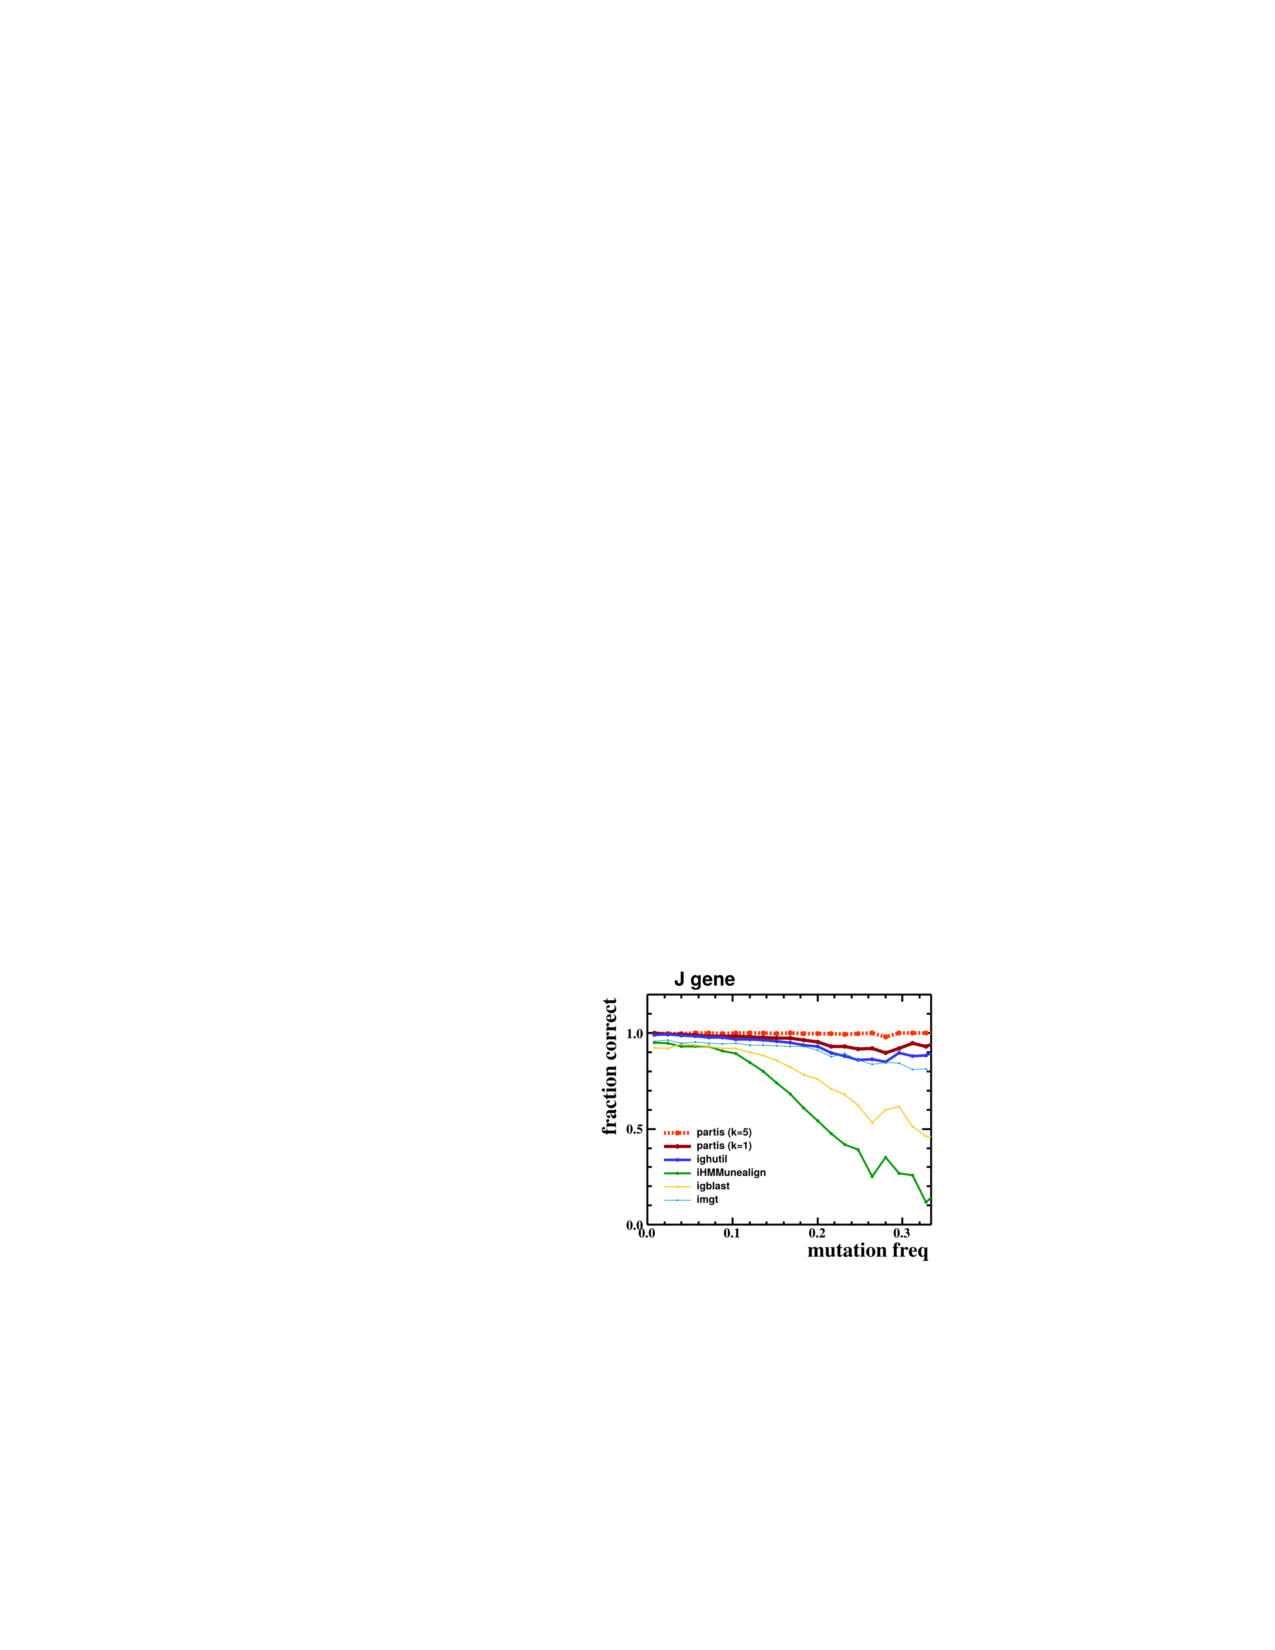
\includegraphics[width=0.5\textwidth]{figures/partis_Jgene_comparison.pdf}
    \caption{
        \label{fig:partis_Jgene_comparison}
        J gene assignment performance for different methods.
        With higher mutational burden most methods struggle to make the correct gene assignments, presumably because of the problem outlined in table \ref{extend_or_not}.
        The HMM method in partis is robust to the mutation burden, and achieves even higher performance by integrate over multiple (k=5) sequences from the same clonal family.
        IHMMunealign and partis are the only HMM methods while the rest are alignment based.
        From \cite{ralph2016consistency}.
    }
\end{figure}


Now returning to the alignment problem exemplified in table \ref{extend_or_not}.
The real shortcoming of using a pure alignment methods is that there is no robust way of deciding what is N/P nucleotides and what is inherited from germline genes, thereby making it very difficult to reconstruct the true naive sequence.
A problem that is well handled by an HMM which will also, as a side effect of calculating the Viterbi path, return the maximum likelihood estimate of the naive sequence.
The speculations were confirmed in the simulation study of Ralph et al.\ that showed substantial performance gains in naive sequence reconstruction using HMMs vs.\ alignment methods, see figure \ref{fig:partis_naiveseq_comparison}.

\begin{figure}
    \centering
    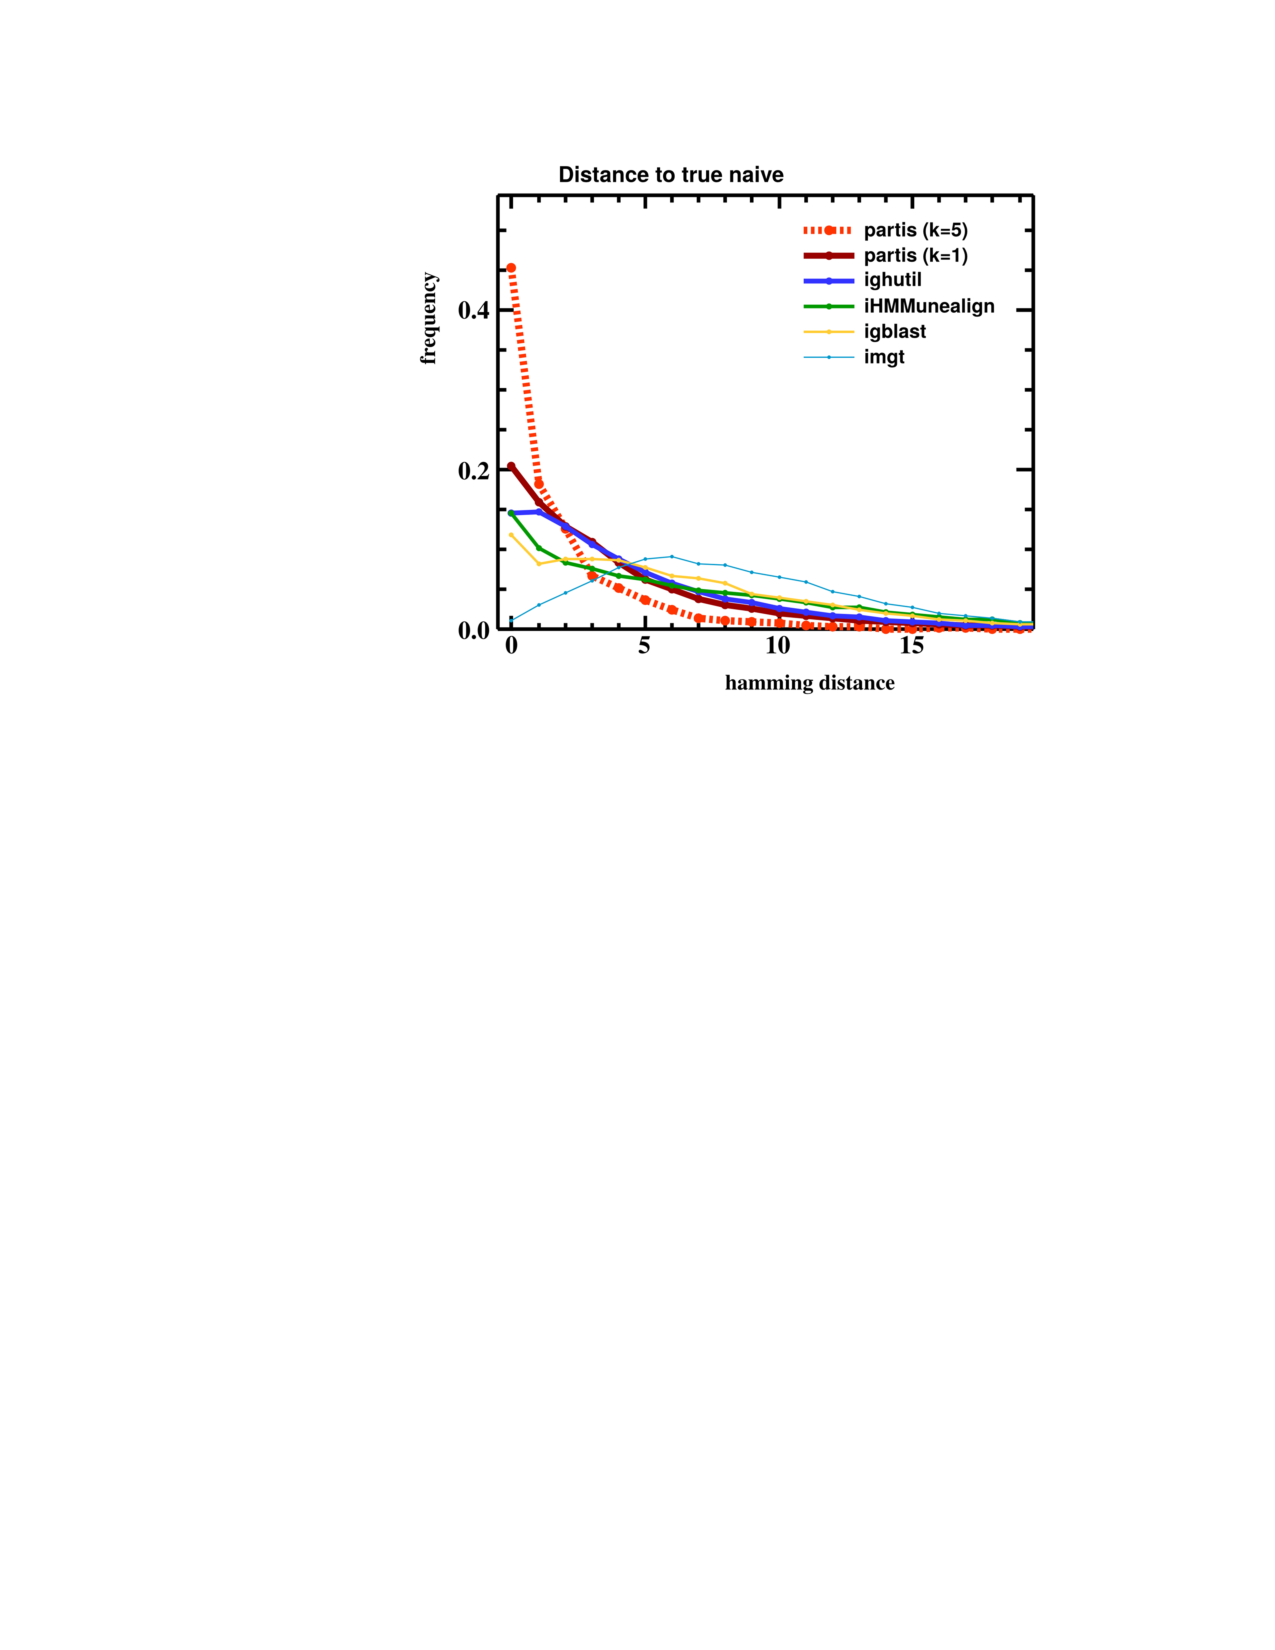
\includegraphics[width=0.5\textwidth]{figures/partis_naiveseq_comparison.pdf}
    \caption{
        \label{fig:partis_naiveseq_comparison}
        Distribution of hamming distances true vs.\ inferred for 30,000 simulations compared across different inference methods.
        There is a clear advantage of using HMM methods like partis, but the largest performance leap is to integrate over multiple (k=5) sequences from the same clonal family (explained in the clustering section).
        IHMMunealign and partis are the only HMM methods while the rest are alignment based.
        From \cite{ralph2016consistency}.
    }
\end{figure}


Next step is to partition the BCR sequences into clusters of sequence related by some definition of relatedness.
These clusters are by some known as clones \cite{gupta2017hierarchical}, which is assumed to mean that they actually came from the same GC reaction.
However as previously discussed the view of GCs as monoclonal is outdated \cite{tas2016visualizing}, so in this work the nomenclature from Ralph et al.\ \cite{ralph2016likelihood} is used, with the assumption that there is sufficient BCR diversity to distinguish clonal families exclusively based on their shared naive sequence.
% Nevertheless the biologically interpretation is that all the sequences in a cluster are highly similar and share the same epitope for binding.
Given this definition a logical first step would be to require that the assigned germline genes in a cluster to match, and indeed such simple clustering has been extensively used.
However in acknowledgement of the uncertainty in assigning the correct D gene, only V and J genes are usually used, and regardless of their allelic variants.
Furthermore the junction length or the CDR3 length has been used as second discriminator and the hamming distance between sequences is usually used as the last discriminator.
Then the procedure for clustering is first to split BCR sequences into buckets with the same V and J gene and junction or CDR3 length, and then sequences in each bucket are clustered based on a distance measure like hamming distance \cite{glanville2011naive}, SHM weighted hamming distance \cite{gupta2017hierarchical} or amino acid based hamming distance confined to CDR3 \cite{jiang2013lineage}.
This method, which will be referred to as "VJ junction agglomeration", has the inherent problem of putting 100\% confidence on the V, J and junction annotations.
However with just moderate SHM there are substantial uncertainties in the annotations and in such cases putting a hard boundary between sequences with different annotations causes problems.
In an example, outlined in figure \ref{fig:VJ_CDR3_agglomeration}, a clonal family would wrongly be assigned into three different clusters (boxes defined by the solid gene lines) if VJ junction agglomeration is used.
Contrarily, if integrating over germline and junctional annotation uncertainties, clustering is not restricted by the point estimate of the gene or allele annotation, and at least has the possibility to merge all red dots into the same cluster.

\begin{figure}[ht]
    \centering
    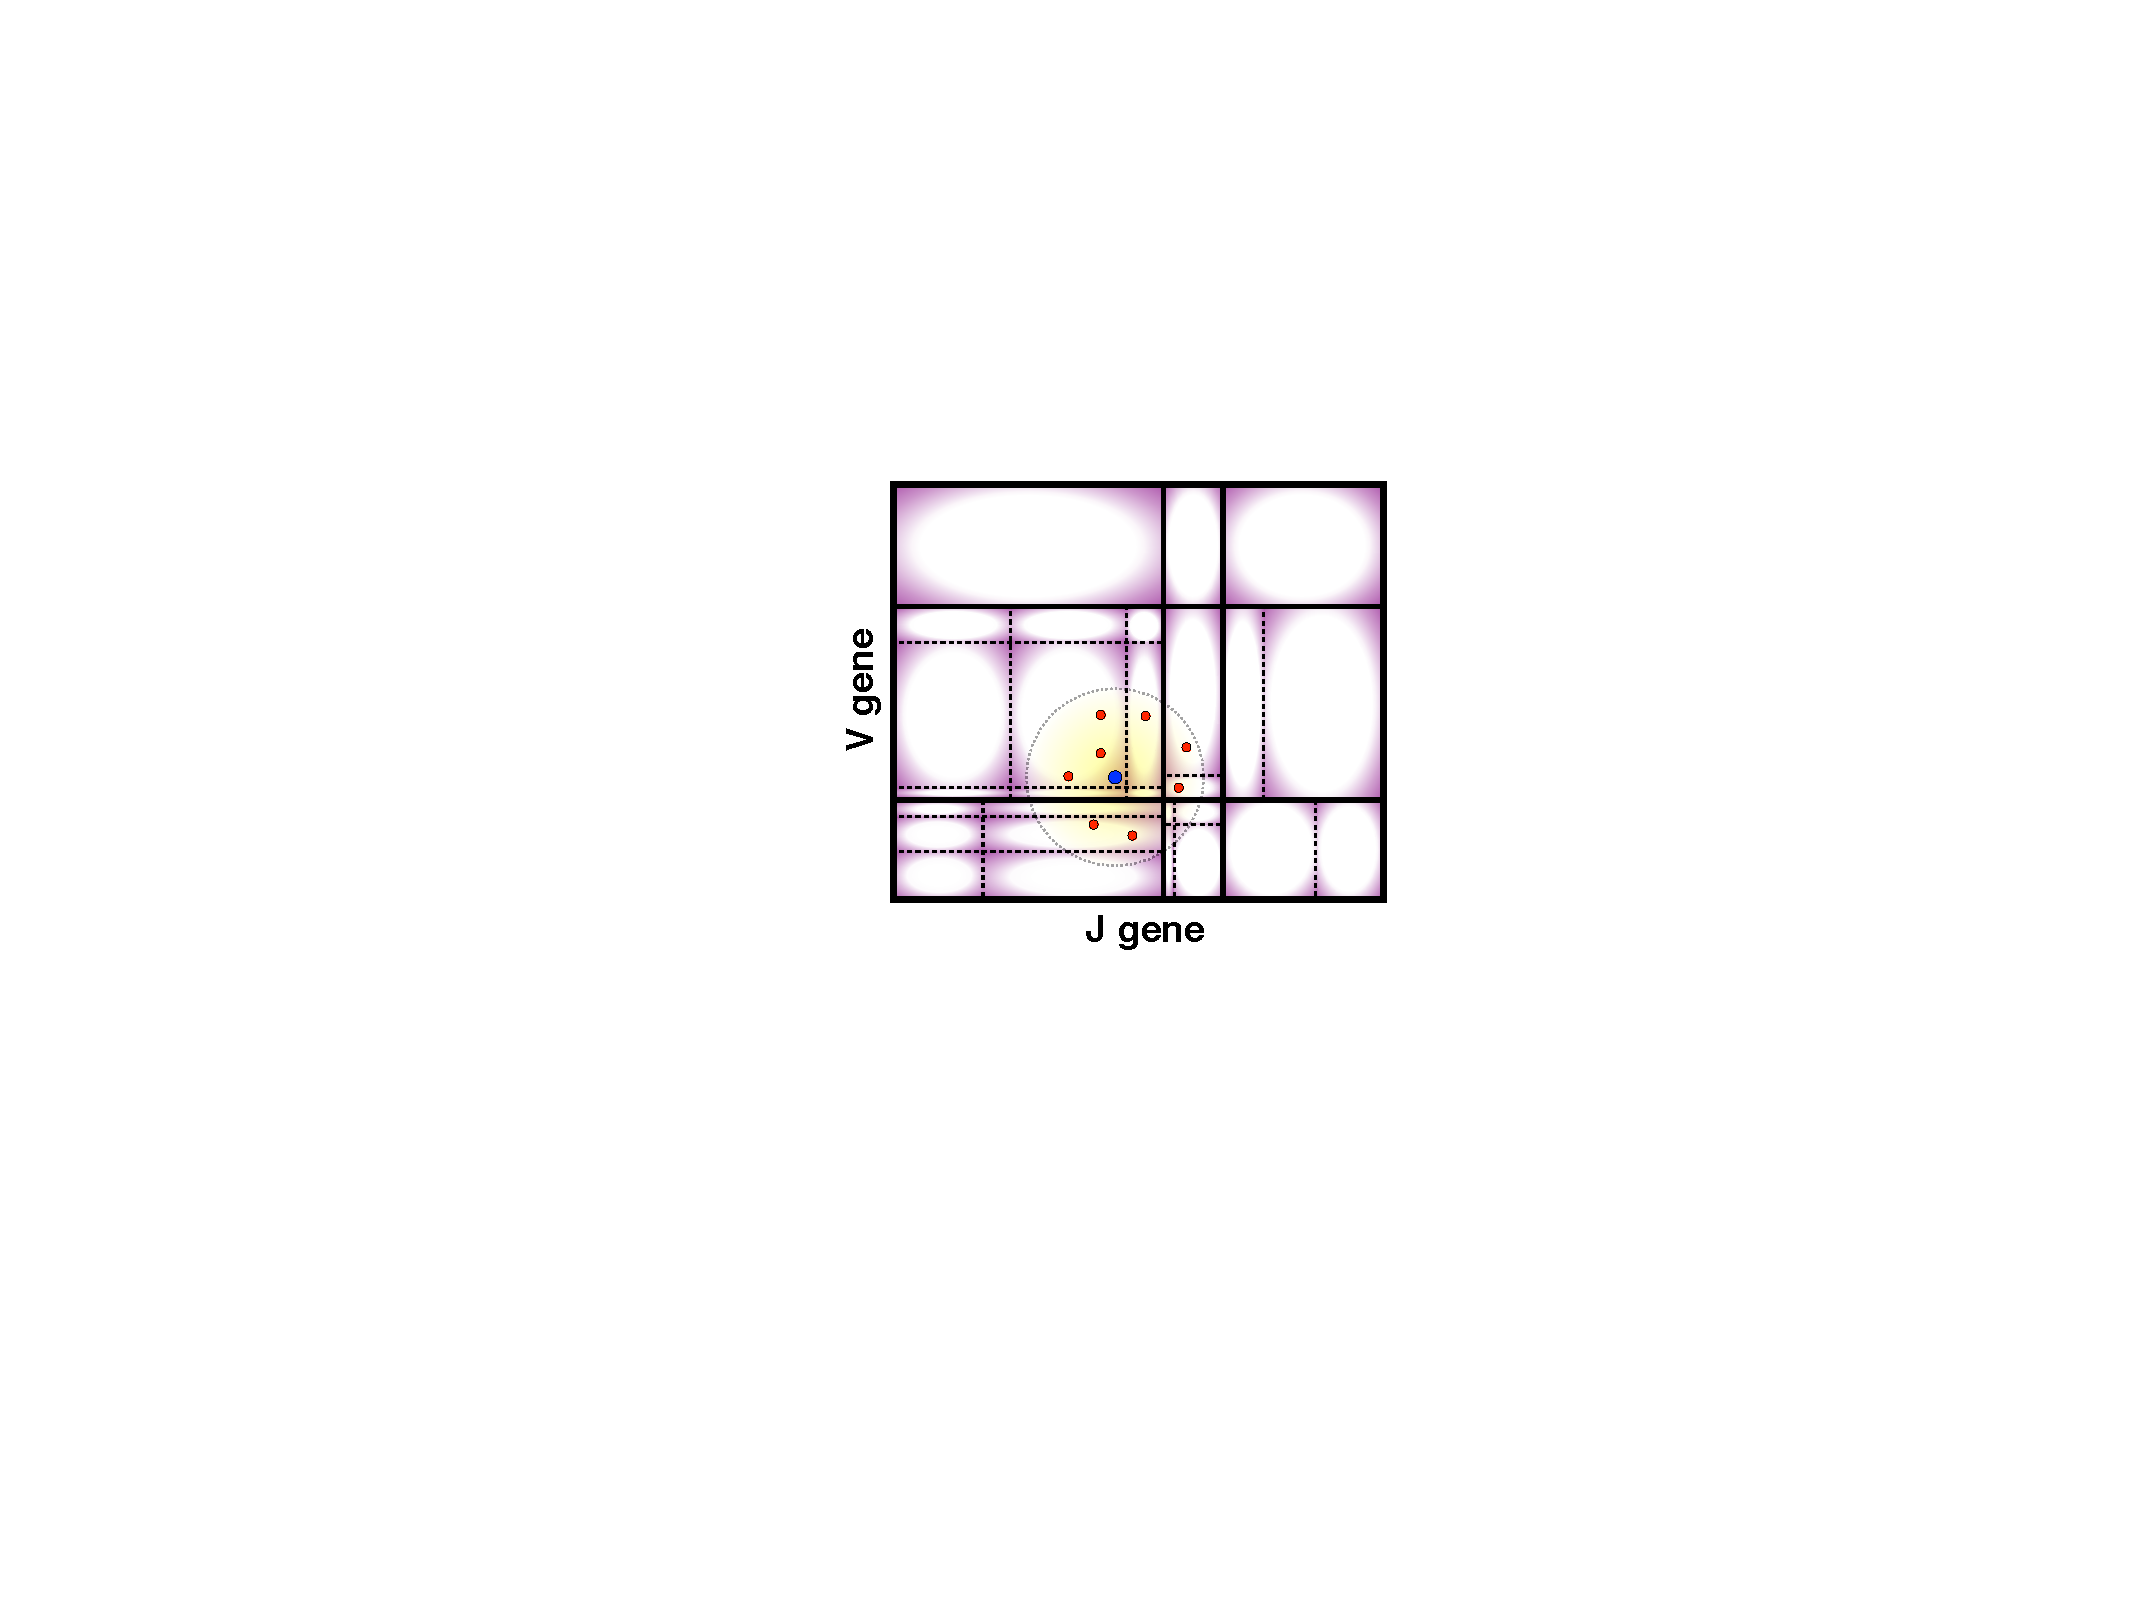
\includegraphics[width=0.5\textwidth]{figures/VJ_CDR3_agglomeration.pdf}
    \caption{
        \label{fig:VJ_CDR3_agglomeration}
        Two dimensional representation of the BCR sequence space that illustrates how V, J and junction point estimates leads to overestimation of the number of clusters.
        Vertical lines represent V genes and dashed lines represent alleles, same for J genes on the horizontal axis.
        Naive sequences with no N/P nucleotides are in the cross section between a V and J allele.
        Colored with purple gradient is the range of junctional diversity extending from the V/J gene combinations, less color means lower probability, all the way to white which is sequences not within the reach of any VDJ recombination.
        The dot in blue represents a naive sequence with its SHM "breadth" marked by a yellow circle.
        Red dots are observed BCR sequences from the clonal family defined by the naive sequence.
    }
\end{figure}


Now it should be clear that the root cause of the clustering problem is propagation of errors in point estimates, i.e.\ ignoring the substantial uncertainty in VDJ annotations of a BCR sequence that has undergone SHM.
When a clustering criterion is based on the point estimate of both the V and J assignment, both the assignment uncertainties are affecting the clustering performance negatively.
The junction length is also problematic to use because it is also just a point estimate, and often estimated from by a problematic alignment method as outlined in the example in table \ref{extend_or_not}.
Lastly, hamming distance is weighting a mismatch in the N/P base region equally likely as a mismatch in the middle of germline gene while there is much more certainty of a real SHM event in the later case.
In the example in figure \ref{fig:VJ_CDR3_agglomeration} VJ junction agglomeration is overestimating the number of clusters and indeed this intuition is also observed in simulation studies \cite{ralph2016likelihood}.

A completely different approach is taken by Ralph et al.\ \cite{ralph2016likelihood}, extending on their HMM framework for germline gene annotation.
They use the naive sequence as a centrality point for clustering, not in terms of hamming distance, but in the terms of likelihood.
The HMM model is conveniently yielding a likelihood function defined over all possible naive sequences for each BCR sequence in the dataset.
With this likelihood function it gets simple to do hypothesis testing based clustering e.g.\ to test whether a set of observed BCR sequences all belong to the same cluster through a common naive sequence ancestor, see figure \ref{fig:partis_clustering-with-likelihood_2}.

\begin{figure}
    \centering
    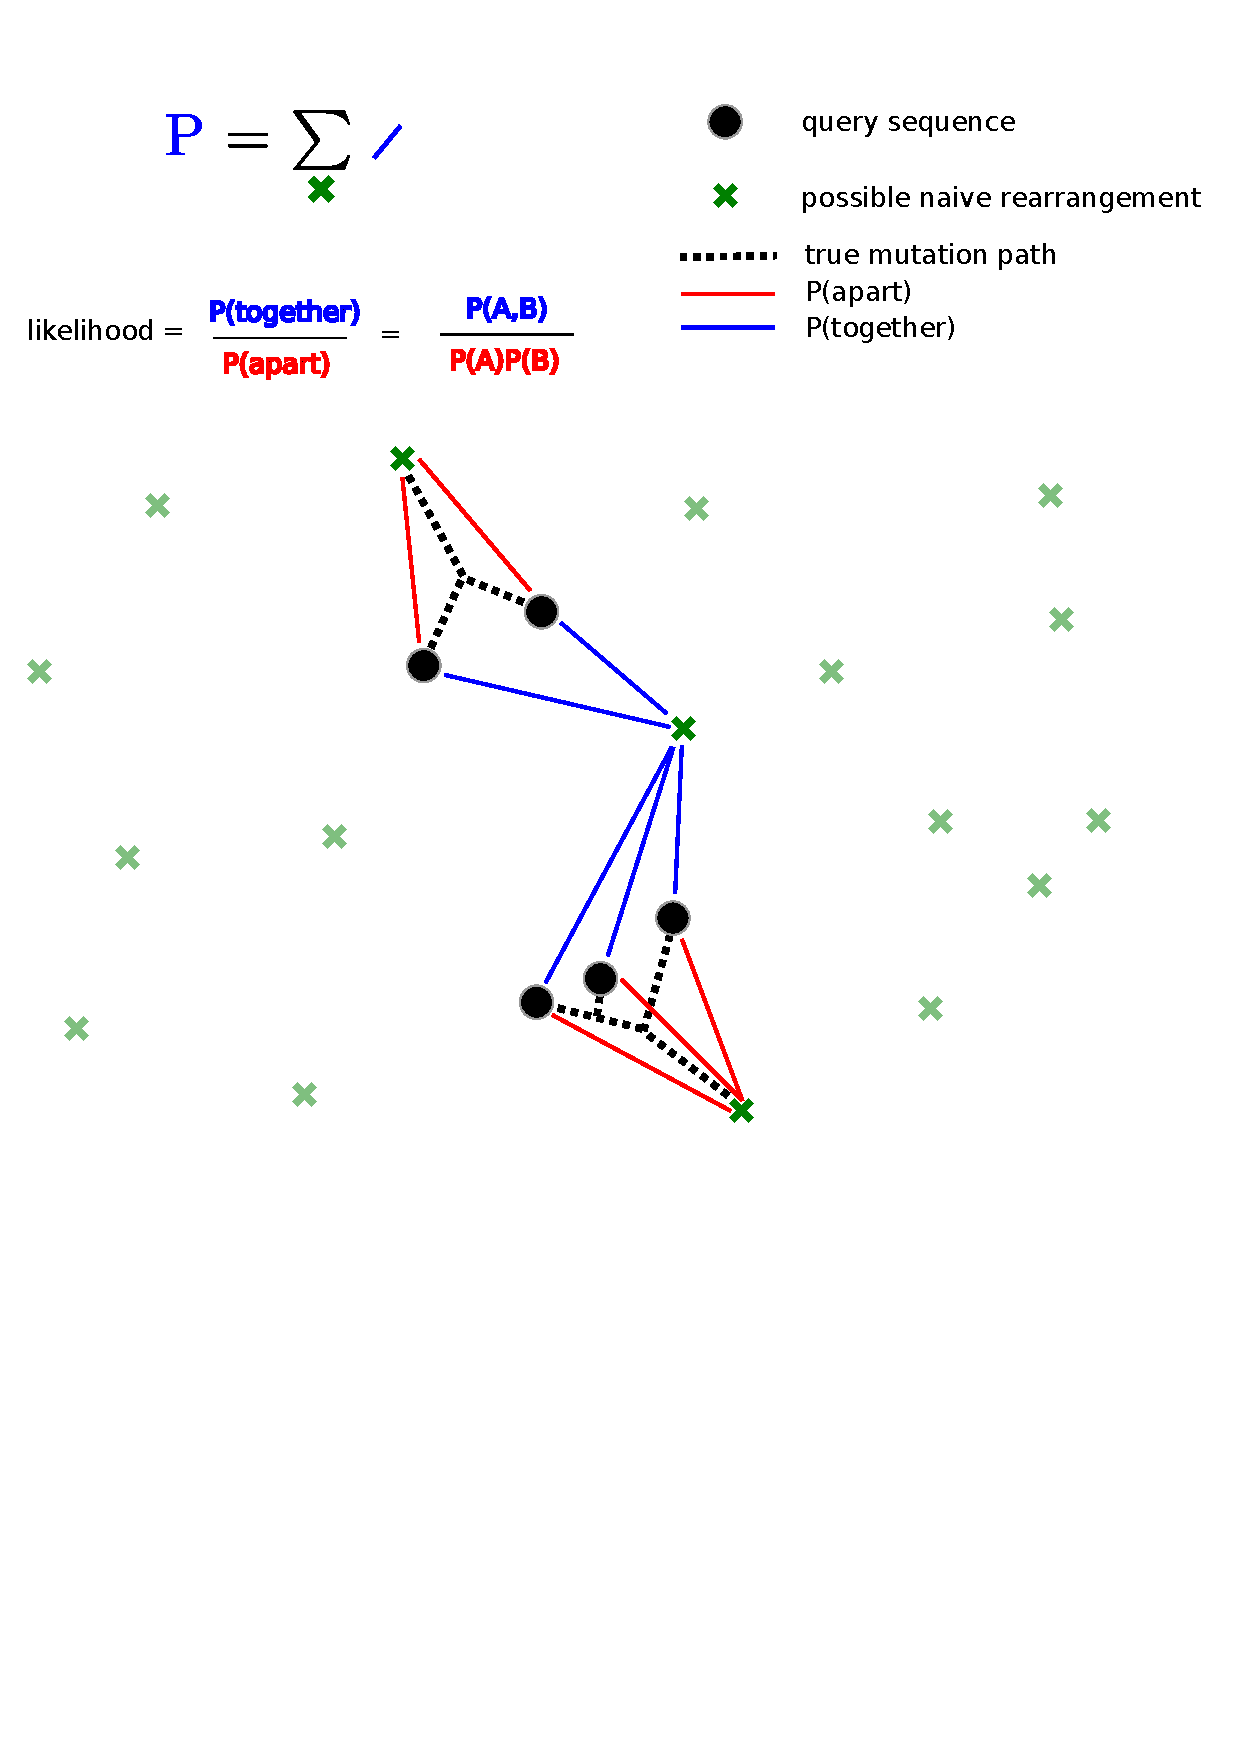
\includegraphics[width=0.7\textwidth]{figures/partis_clustering-with-likelihood_2.pdf}
    \caption{
        \label{fig:partis_clustering-with-likelihood_2}
        Likelihood ratio test to decide whether to merge a set of sequences into a cluster or not. Figure credit: Duncan Ralph.
    }
\end{figure}


Notice that the likelihood ratio test based clustering in partis is centered around the likelihood of the proposed naive sequence and the thus allow for merging of sequences with different VJ gene annotation point estimates.
When clustering has run to an end the final annotation of each sequence will change to reflect a common VDJ rearrangement for all cluster members.
The shared information among cluster members makes inference of the naive sequence much more probable because all sequences can be integrated into the same HMM, referred to as multi-HMM in Ralph et al.
The strength of using multi-HMM to infer a naive sequence is obvious from a theoretical stand-point.
Multiple sequences are regarded as multiple independent observations of the same mutation process and this will increase the probability of the germline annotation, but more so, it will increase the odds of observing the true naive sequence in the N/P junction.
This claim is supported by striking improvement in both annotation (figure \ref{fig:partis_Jgene_comparison}) and naive sequence inference (figure \ref{fig:partis_naiveseq_comparison}) for just 5 clonal family sequences (k=5).

The advantages of HMM based BCR annotation and clustering should now be clear and therefore all germline annotation, naive sequence inference and clustering of BCR sequence throughout this work was done with the partis software (\url{github.com/psathyrella/partis}).











\section{Phylogeny of a clonal family}
The problem of determining phylogenies is the problem of reconstructing the unobserved evolutionary history, usually, using only a sample of states at a single time point.
Since there are no observations of the events prior to the sampling time we cannot be certain about a phylogeny.
The problem turns into an inference problem.
For B cells this translates into finding the evolutionary history starting from a naive B cell, progressing through rounds of SHM in the GC reaction and finally getting sampled at some time $t$.
The only information available is the BCR sequences at the sampling time.

To represent the process of cell division and apoptosis in the GC it is convenient to use a tree.
The root of this tree is the naive B cell, a branching event is a cell division and a terminal leaf is a B cell that have died.
The tree model of evolution is also a useful way of representing relationship among sequences e.g.\ some sequences which are all members of the same tree clade share a common ancestor and most likely are more similar than some other sequence not included in this clade.
The phylogenetic tree should be viewed as a model framework used to describe the evolutionary process, the details that goes into the model framework depends on the problem at hand.



\subsection{Parsimonious tree inference}
Now given that the evolution is following a tree model, the model for inferring the topology must be specified.
A classical method for inference is to maximize tree parsimony.
Motivated by Occam's Razor the best tree is simply the tree that with the fewest changes explain the observed data.
Practically this is done by calculating the tree parsimony score with Fitch's algorithm \cite{fitch1971toward} and then finding the tree with the lowest score.
The parsimony score of a tree ($T$) can be calculated as a sum of all the scores at each site ($p_i$): $S(T) = \sum_{i=1}^m F(p_i | T)$.

With a parsimony score function the possible tree space can be searched and the maximum parsimony (MP) tree can be found.
Tree space can be searched exhaustively only with few taxa but everything above 10 taxa has more than tens of millions of tree making it practically impossible to search exhaustively \cite{felsenstein1978number}.
The branch and bound algorithm is a way of decreasing search space but still finding the best solution \cite{hendy1982branch}, however even with this hill climbing methods have to be used.
In a hill climbing tree search various heuristic tree moves like, nearest neighbor interchange (NNI), subtree pruning and regrafting (SPR) and tree bisection and reconnection (TBR) are used to explore widely around the tree space.

It it clear that the MP method for tree inference is very simple and while this will work in some applications the criterion of maximum parsimony is not strictly how evolution works.
In cases with rate heterogeneity due to a biased mutation processes or selection some sites might evolve much faster than others and this makes the parsimony assumption of equal weight on all substitutions break.
Such complex processes are not accounted for in the MP method making it prone to errors, but even with the simplest sequence evolution process theoretical arguments by Felsenstein have shown that parsimony is inconsistent \cite{felsenstein1978cases}, and since adding parameters to model a complex process is not readily compatible with parsimony, most researchers have turned to model based tree inference.




\subsection{Model based tree inference}
As an alternative to maximizing the parsimony a likelihood function could be formulated to return the likelihood of the data given the tree. Then the problem turns into finding the most likely tree, referred to as the maximum likelihood (ML) tree.
The likelihood function is conditioned on a tree with branch lengths representing distances in a continuous mutation process driven by a mutation rate.% determined by a matrix of substitution rates.
Using gradient decent tree parameters like branch lengths can be adjusted to their ML estimates.
To accommodate more advanced things such as differences in substitution rates, e.g.\ higher rate of \texttt{T->G} than \texttt{T->A}, a rate matrix can be defined.
If the data is at DNA level the rate matrix contains all possible substitutions between DNA characters.
Examples such matrices: the F81 model \cite{felsenstein1981evolutionary} or the widely used general time reversible (GTR) model \cite{tavare1986some}.

DNA substitution models are not aware of protein encoding and therefore does not explicitly discriminate between synonymous and non-synonymous mutations, something that is otherwise crucial for proteins under tight selection.
Therefore it might be useful to translate a DNA sequence into its protein sequence and then use an amino acid substitution matrix like PAM \cite{dayhoff197822}, BLOSUM \cite{henikoff1992amino} or others.
Information is lost in the translation process so if an amino acid model is to replace the DNA model, information loss needs to be outweighed by the gain in performance.
Alternatively a codon model is defined on DNA level, but with DNA level substitutions working on units defined by protein encoding codons.
In this way a codon model will both account for a difference in the rate of synonymous and non-synonymous substitutions and the rate difference between amino acids.
Two popular choices for a codon model are GY94 \cite{goldman1994codon} and MG94 \cite{muse1994likelihood}.



\subsubsection{Bayesian phylogenetics}
In the ML framework both tree, branch length and substitution parameters are all point estimates adjusted to maximize the likelihood function, but point estimates might not always be desirable.
E.g.\ when information like time or rate is to be extracted from a tree then a single point estimate is not very useful because the variance of such estimate is unknown.
Bayesian phylogeny addresses this challenge by integrating over the distribution of trees, branch lengths and substitution parameters by Monte Carlo sampling.
When sampling has converged the resulting posterior distributions of all parameters can be used to express confidence in the maximum a posteriori (MAP) estimate e.g.\ by providing the high density interval (HDI) along with the MAP estimate.
The real drawback of Bayesian phylogeny is that sampling can make runtime much slower than a similar ML problem.
There can also be a problem of reaching convergence in cases where sampling is difficult.





\subsection{Ancestral sequence reconstruction}
As a side result of inferring a phylogeny it is also possible to reconstruct the sequence of those nodes that are internal and unobserved in a tree.
This process is known as ancestral sequence reconstruction (ASR).
For the MP algorithm these ancestral states are part of the tree inference and found via Fitch's algorithm, but for a model based method ancestral sequences must be estimated by extracting the maximum likelihood estimate of the sequence at each internal node.
ASR on ML trees can either be done as a marginal or a joint reconstruction.
In the marginal case each node is reconstructed independently from one another, found as the ML estimate without fixing the sequence of any of the other internal nodes.
Notice that when one ancestral sequence is found this will change likelihood function for the tree and thereby affecting all the other internal node.
This effect is ignored in marginal reconstruction but accounted for in joint reconstruction where the problem is to find the ML estimate of all the ancestral sequences jointly.

ASR is an important way of exploring the evolutionary trajectory and behaviour of ancient proteins.
It has been used to investigate the specificity of the important cancer drug type kinase inhibitor \cite{Wilson2015-vi} and studying evolutionary trajectories of broadly neutralizing HIV antibodies \cite{Doria-Rose2014-vi}.
Yet there has been little validation of ASR methods partly because it is difficult to test experimentally.
An exception to this was enabled by a clever study design made by Randall et al.\ \cite{randall2016experimental}, using a controlled system of evolution on a single gene with sampling of ancestors, they could experimentally validate ASR inference methods on the using only the final time point.
Results showed high accurary of 97.17-98.88\% correct reconstruction and only small difference between chosen methods.




\subsection{Genotype collapsed tree}
While B cells in a GC reaction are having a high mutation rate there are still many B cell with the same genotype.
Especially after a clonal expansion many B cells will have the same genotype, and furthermore ancestral B cells might have the same genotype as their descendents.
BCR clonal family sequences are generally of low complexity and not very divergent, but because there are many B cells in a GC their phylogenetic trees are seemingly complex with hundreds to thousands of taxa.
To reduce this complexity we use the concept of a genotype collapsed tree (GCtree).
In a GCtree B cells with the same genotype are merged into a single node carrying their total abundance and a leaf descending from a B cell with the same genotype is merged upwards, see figure \ref{fig:GCtree_illu}.

\begin{figure}[!ht]
    \centering
    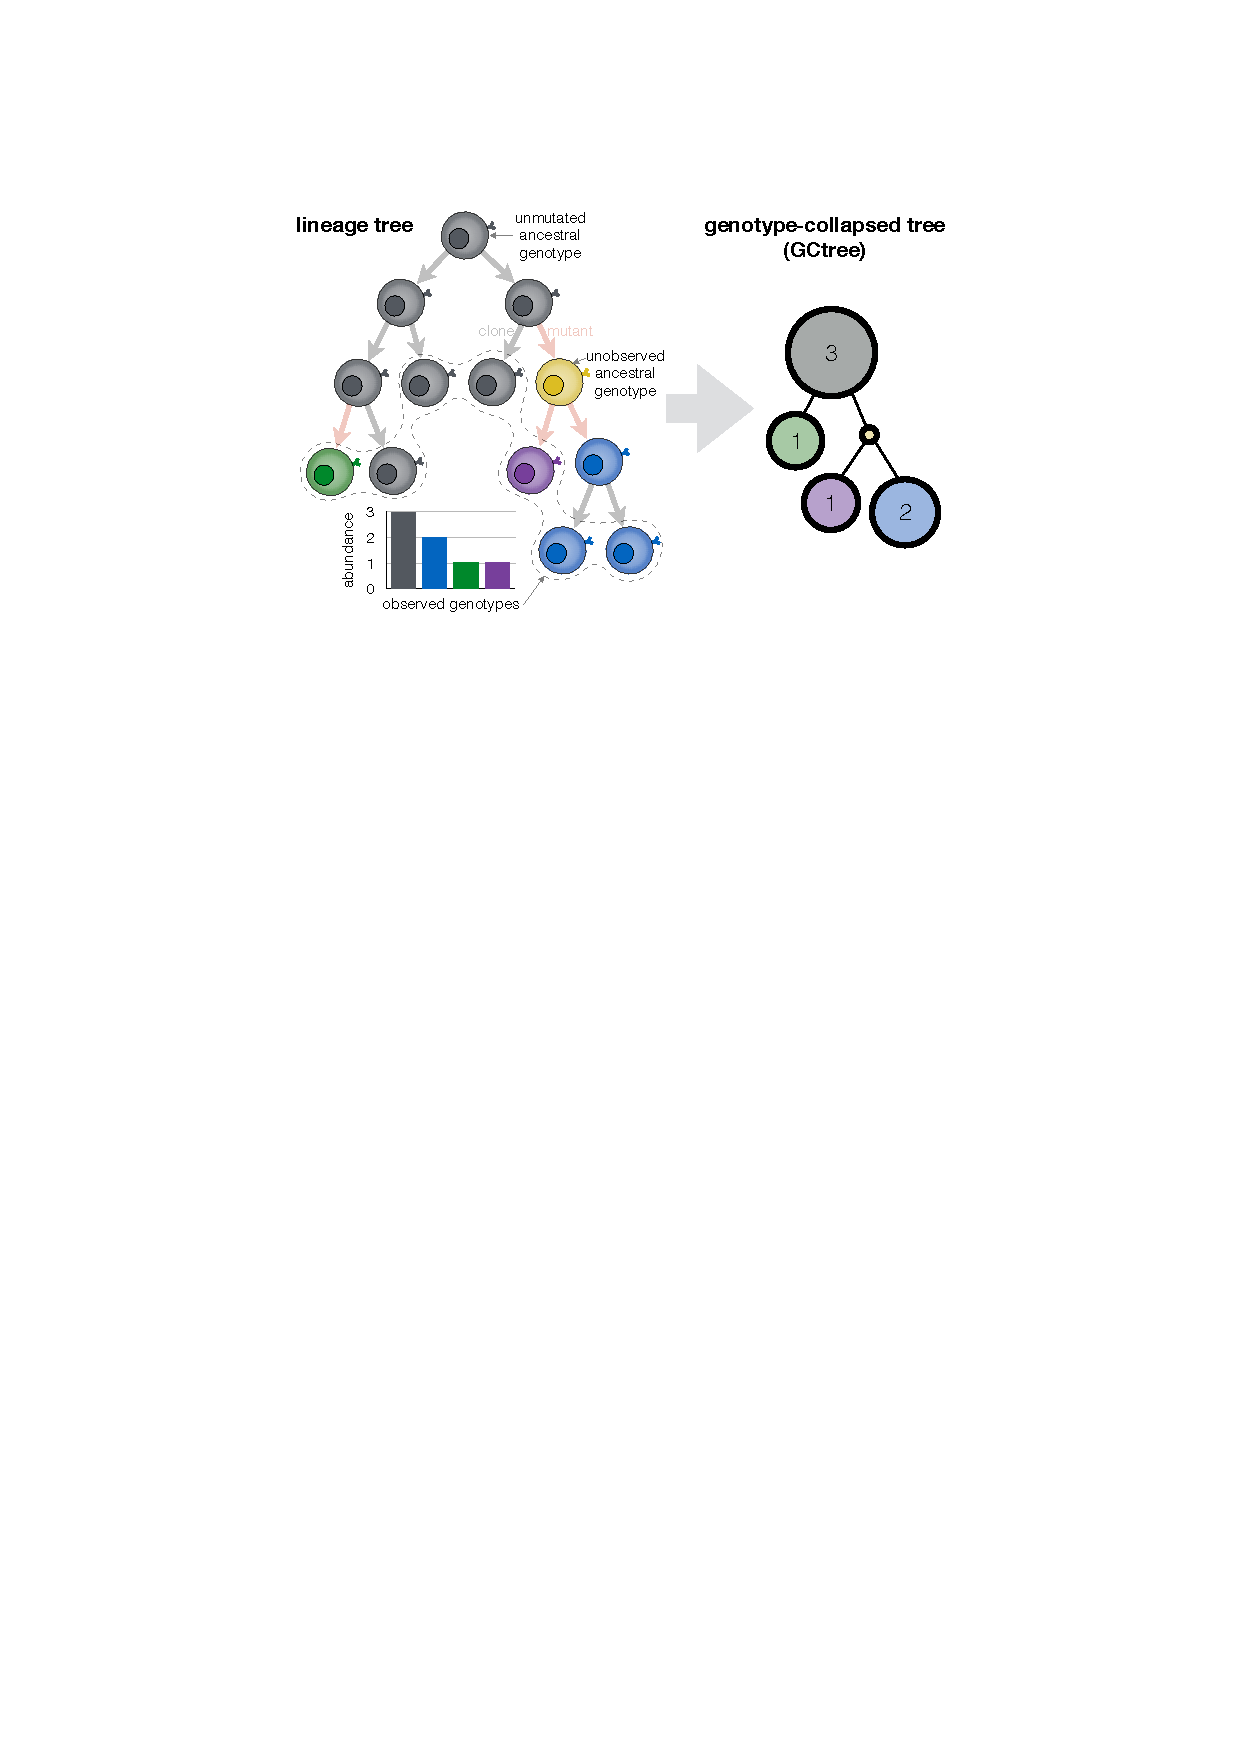
\includegraphics[width=0.7\textwidth]{figures/GCtree_illu.pdf}
    \caption{
        \label{fig:GCtree_illu}
        Genotype collapsed tree.
        Observed cells fenced by a dashed line are getting deduplicated and the total abundance is recorded.
        Next the tree is collapsed upwards, merging cells of the same genotype, ending up with the tree to the right.
        Figure credit: William S. DeWitt.
    }
\end{figure}


We find that the GCtree gives a good visual overview of the BCR phylogeny enabling interpretations such as recent clonal bursts, fitness advantages etc.
In the rest of this work all trees will be shown as a GCtree using custom tree plotting from the ETE package \cite{huerta2016ete}.
Figure \ref{fig:collapsed_tree_example} is an example of how a standard phylogenetic tree is collapsed and represented in GCtree format.
Embedded in the GCtree visualization is a number of traits: genotype abundance is annotated in the middle of each node and proportional to the node size, dashed branches represents synonymous mutations while fully drawn lines are non-synonymous, branch length is proportional to the hamming distance between nodes and branch thickness is proportional to the number of amino acid differences.

\begin{figure}[!ht]
    \centering
    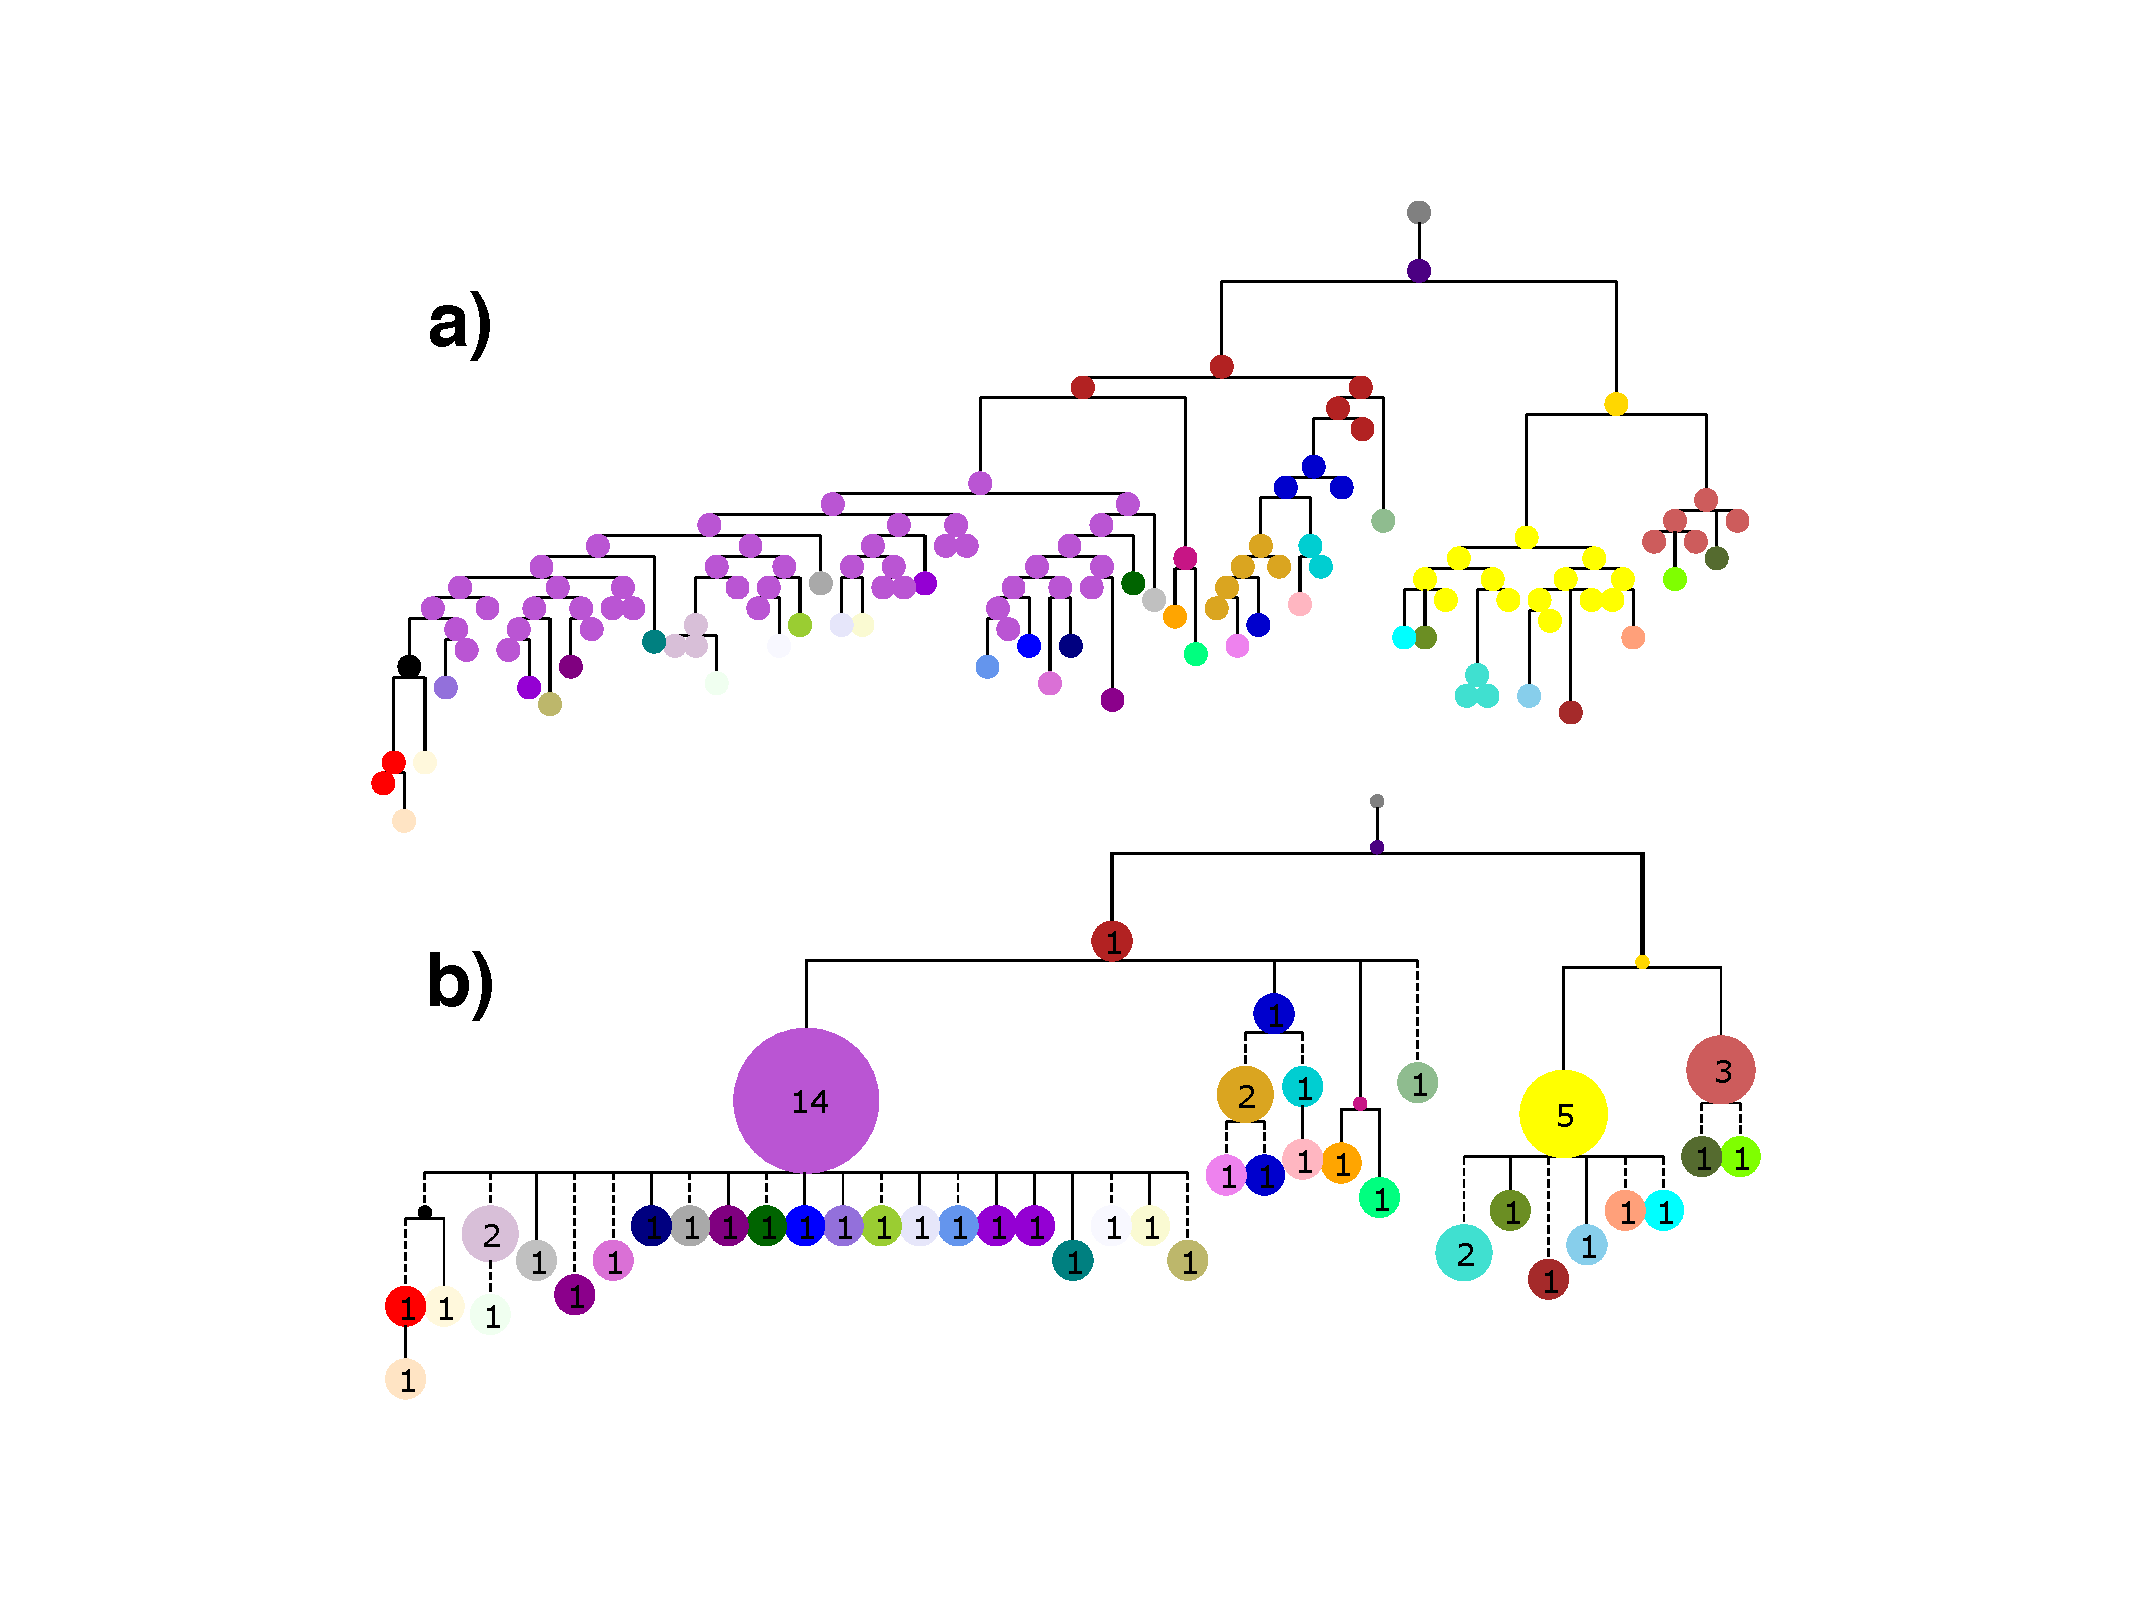
\includegraphics[width=0.7\textwidth]{figures/collapsed_tree_example.pdf}
    \caption{
        \label{fig:collapsed_tree_example}
        Genotype collapsing of a simulated tree with node coloring according to genotype.
        In a) a full lineage tree showing a simulation of several rounds of replication.
        Only the leafs are sampled at the end of the simulation and collapsed into the GCtree in b).
        The GCtree shows the leaf abundance of each node by way of node size and the integer in the middle of the node.
        In the GCtree synonymous mutations are indicated by dashed branch lines, branch length is reflecting the hamming distance between nodes at DNA level and solid branch line thickness reflects the number of non-synonymous mutations.
    }
\end{figure}





\subsection{Clonal family tree}
Most often the source of BCR sequences is HTS data generated from bulk RNA, extracted from peripheral blood mononuclear cells (PBMCs).
Clonal family relationships therefore needs to be inferred by means of clustering before sequences can be inputted to phylogenetic tools.
An automated pipeline can be envisioned, with HTS data as input and inferred clonal family trees as output.
One attempt at this task is the publicly available ImmuneDB \cite{rosenfeld2017immunedb}.
Using relatively simple clustering and inference of naive sequences ImmuneDB still has room for improvements, but the concept remains extremely important as a way of aiding the interpretation of Rep-Seq data.
On the conceptual side of the clonal family tree representation is it possible to map meta information about binding affinity, cross reactivity, self-binding etc. back to individual trees to get a detailed picture of the evolutionary process at a single cell level.







\chapter{Simulating sequences undergoing affinity maturation}

\section{Introduction}
Antibodies have an important role in adaptive immunity by specifically binding to and neutralizing invading pathogens like bacteria and viruses.
Developing specific antibodies involves reactions across the entire immune system, but it is B cells that mature and secrete antibodies, after undergoing several rounds of selections in the bone marrow and the germinal centers (GCs).
B cells undergoing GC affinity maturation express antibodies as B cell receptors (BCRs), and these are subject to a strict selection scheme, where many different factors come into play e.g.\ antigen affinity, receptor expression -and folding, codon choice affecting translation rates and affinity to self antigens.
All these factors leads back to the same thing: the ability to bind antigen, and this is measured by nearby T cells, which will be affecting the mutual probabilities of proliferation or apoptosis \cite{Bannard_Cyster_2017}, \cite{victora2012germinal}.
As an example in a GC there is a direct T cell mediated selection for higher BCR affinity by means of sequestering more antigen.
Selection against binding of self antigens is mediated by the fact that binding self antigens will block binding of pathogen antigens, resulting in decreased T cell help.
Therefore, in its most simple way, affinity maturation is driven by affinity towards the presented antigen, and all the effects also attributed to selection, like folding, stability and aggregation, is selected by means of their shared effect on affinity.

Affinity maturation is a strong selective pressure imposed on the B cell evolution, and this poses a challenge to phylogenetic reconstruction.
To validate the correctness of phylogenetic methods simulation studies are among the most important tool.
Classically done by randomly permuting a sequence along a tree or sampling mutations from a distribution of substitutions, but simulations can also be configured to have selection.
%EM I suggest lit review be a little expanded, and clarify that you are talking about nucleotide sequence. There are other things to cite-- see https://paperpile.com/shared/dAcoWo
%EM Also suggest distinguishing from the type of modeling done in https://paperpile.com/shared/UTRt7K, e.g.
While many groups have simulated affinity maturation over time \cite{Reshetova_2017}, \cite{Balelli_2016}, \cite{Childs_Baskerville_Cobey_2015}, there have been no example of affinity centric simulations on single sequence level, and indeed most GC simulation studies treat the BCR sequence as a hidden state to focus on the summary statistics of the whole GC.

We propose a simple model of affinity maturation that models sequence fitness as a function of BCR affinity.
If the BCR affinity is high it means that the B cell will endocytose a lot of antigen, thereby getting plenty of T cell help to decrease the changes of undergoing apoptosis while increasing the chances of proliferation.
Alternatively, if the BCR affinity is low no antigen will be endocytosed and chances are high that the cell will undergo apoptosis.
Under this setup it is not the absolute affinity that matters, but rather the affinity relative to the affinities of all the competing cells in the whole GC, held against the total amount of antigens to compete for.
By modularizing the simulation code we first make a model for a neutral branching process, and then make an optional affinity selection step that works in conjunction with the neutral process used to introduce substitutions.

The purpose of the presented simulation method is to generate more realistic sequence simulations of clonal families to be widely used for assessing the performance of phylogenetic methods.
The model is supposed to capture the most influential effects of affinity maturation without being a detailed mechanistic model, although be sufficient to recapitulate the features of real GC sequence data.






\section{Methods}

\subsection{Neutral branching process}
A neutral branching process, independent from the later described affinity model, was setup as a reference point for simulation.
It can be viewed as a model of cell divisions, where at each generation a cell can either die or produce a number of offspring, and each offspring has some probability of carrying a mutation.
The neutrality assumption lies in the fact that the mutations introduced will have no fitness effect in later generations.
The root sequence is given at initialization as a starting point to evolve through a stochastic branching process, that also includes stochastic introduction of mutations at each generation.
The branching process is controlled by an arbitrary discrete distribution, which in this case we take to be a Poisson distribution, due to its convenient mathematical properties.
Thus, in the below sections the branching process is controlled by a $\operatorname{Pois}(\lambda)$ progeny distribution.
%Furthermore at each generation all progeny cells will undergo a mutation process determined by discrete distribution, again we use Poisson.
%The number of nucleotide mutations is drawn from $\operatorname{Pois}(\lambda_0)$ and then introduced sequentially into the sequence.
Furthermore at each generation all progeny cells will undergo a mutation process with the number of nucleotide mutations drawn from $\operatorname{Pois}(\lambda_0)$ and then introduced sequentially into the sequence.
Sequential mutations allow the possibility of back mutations.
Mutations can be introduced using a uniform probability over all sites, but because it is well known that BCR sequences do not mutate uniformly at random \cite{Yeap2015-nl}, we used an empirical approximation of the mutation context sensitivity, called S5F \cite{cui2016model}.
The S5F model describes mutability of the middle base of all 5-mer DNA motifs, and for each motif the base preferences given a mutation i.e.\ if a random process chooses to mutate the 5-mer \texttt{AAAAA}, then the S5F model will provides a list of probabilities for each middle base substitutions, either $P(\AAAAA \rightarrow \AATAA)$, $P(\AAAAA \rightarrow \AAGAA)$ or $P(\AAAAA \rightarrow \AACAA)$, probabilities summing to 1.
A 5-mer mutability cannot be used directly on sites at the start or end of a sequence because of missing context.
We fill in missing context with the unknown base, N, and average over all possible motifs fitting into this ambiguous context.

Termination of the neutral branching process is enforced in either of three ways: 1) by simulating under a subcritical process ($\lambda < 1$) \cite{gwp} and following it until extinction, 2) by using a stopping time $T$, or 3) by stopping after a max population of $N$ has been reached.
Leaves are sampled from last time point, or in the case of 1) only terminated leaves.
In addition we introduced a parameter for down-sampling the cell population to $n$ cells.
Down-sampling allows for emulating the incomplete sampling of a GC cell population, which is expected to happen in HTS data due to fall out during PCR, sequencing, quality control steps and limited sampling e.g.\ in the case of data from PBMCs.
The five parameters of the model is tabulated in table \ref{neut_constants}, but only one of the stopping criteria can be used in a run, effectively making it a four parameter model.

\begin{table}[ht]
\centering
\begin{tabular}{ll}
Parameter    & Description \\ \hline
$\lambda$ & $\operatorname{Pois}(\lambda)$ progeny distribution \\
$\lambda_0$ & $\operatorname{Pois}(\lambda_0)$ mutation distribution \\
$T$ & Stopping time \\
$N$ & Stopping number of sequences \\
$n$ & Down-sampled number of sequences
\end{tabular}
\caption{
\label{neut_constants}
    Parameters used in the neutral branching process simulation.}
\end{table}






\subsection{Simulations with affinity selection}

\subsubsection{Model concept and biological assumptions}
In the following sections the model for affinity selection will be described in detail, but lets first make some basic assumptions to keep later definitions simpler.
First of all the system we intend to model is the affinity maturation that is happening in the GC reaction, as guided by the BCR's affinity towards a target antigen.
A real GC reaction is seeded with 50-200 naive B cells and is therefore in its initial state highly polyclonal \cite{tas2016visualizing}.
However, during the extend of a GC reaction the lineages descending from these seeds gradually die off \cite{tas2016visualizing} and the GC may even reach full monoclonality, in which a single lineage comes to dominate.
Because we are interested in relatively large lineages that eventually lead to immune memory, we thus make the simplifying assumption that the simulated GC is monoclonal seeded by a single cell.
Although polyclonality could be integrated into the simulation method, this would not change the simulation results significantly and therefore prefer to keep the description simple.
In this model it is the BCR amino acid sequence that is under selection, thus we ignore the possible fitness effects of synonymous mutations.
Although these might affect transcription and/or translation rates, we ignore these more minor effects to simplify the model.

The system is modelled as a GC with constant volume and constant total concentration of antigen which a number of B cells compete to bind, summarized here and detailed below (figure~\ref{fig:simulation_figure}).
Those B cells that have high affinity BCRs will bind more antigen and these B cells will be more likely to undergo proliferation, while the opposite is true for those BCRs with low affinity.
When the binding equilibrium has been reached the progeny distribution for a B cell is evaluated given the amount of antigen bound.
Affinity of a progeny cell is a function of the BCR sequence, as defined by the BCR fitness landscape, and after cell division the binding equilibrium is updated according to the progeny cells and their affinities.
Finally when all B cells have been evaluated a new round of selection starts.

\begin{figure}[ht!]
    \centering
    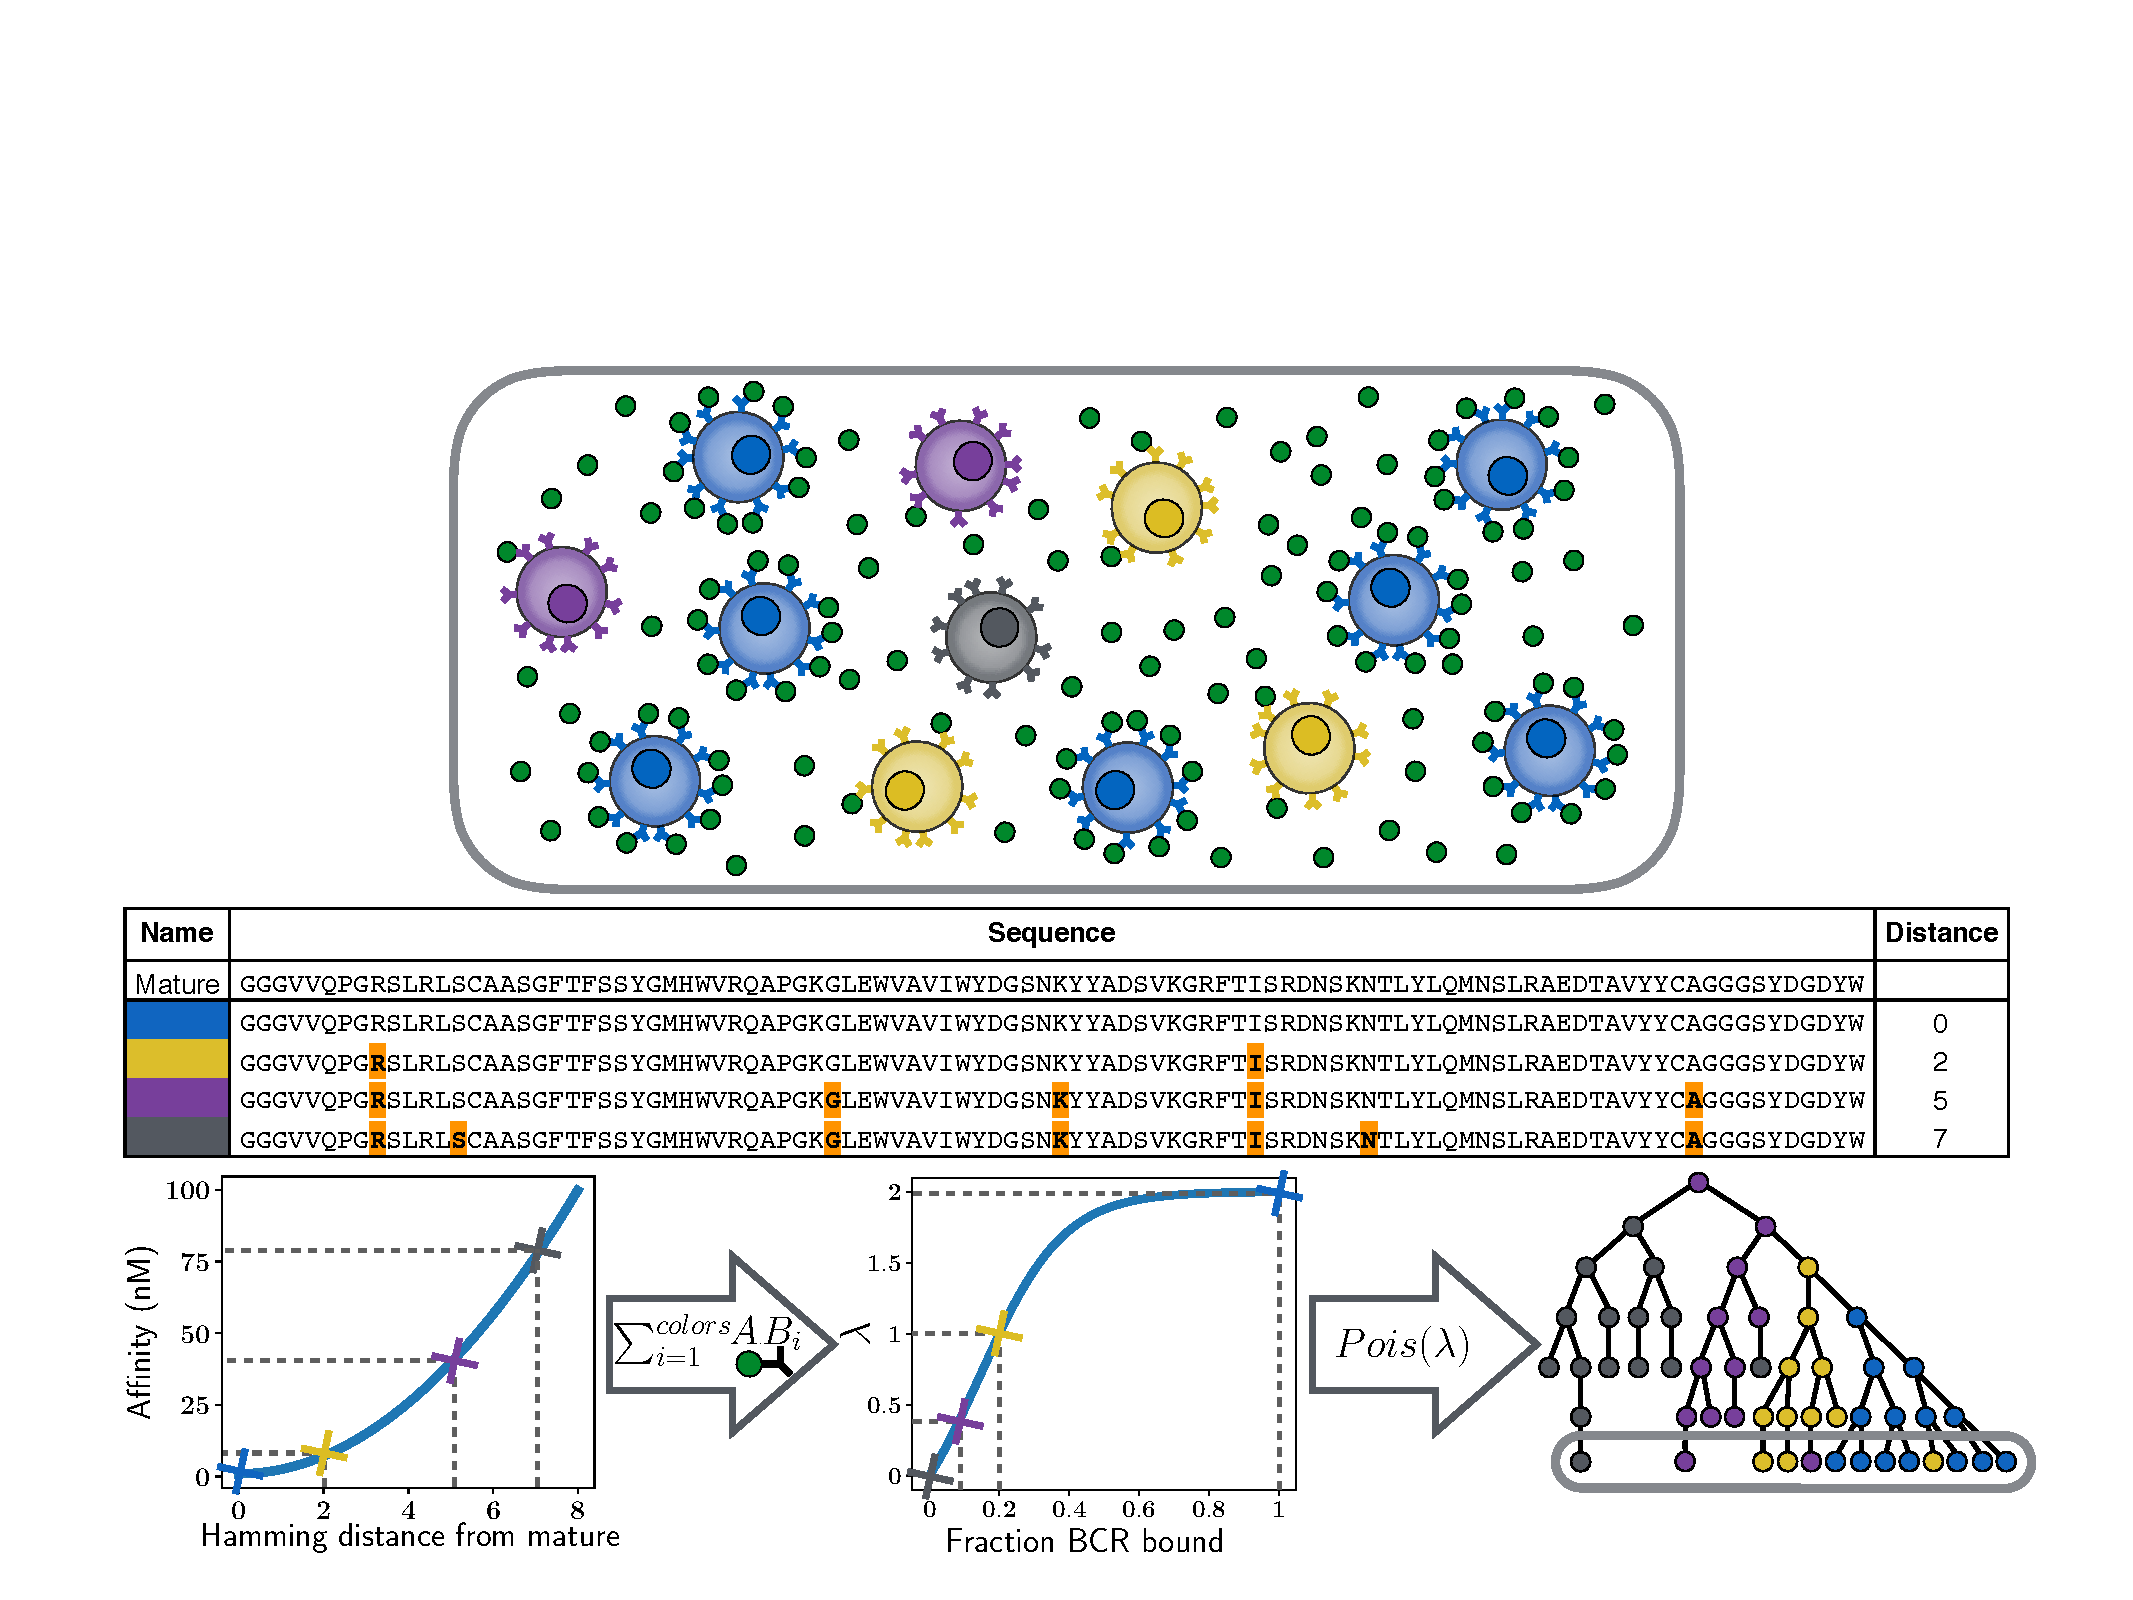
\includegraphics[width=1\textwidth]{figures/simulation_figure.pdf}
    \caption{
        \label{fig:simulation_figure}
        Simulation overview.
        The system is considered as a closed environment with free floating antigen and a number of B cells presenting BCRs on their surface, as illustrated in the top panel.
        Different colors correspond to different BCR sequences with different affinities.
        In the middle panel a sequence alignment shows how the different BCR sequences and their distance to the target mature BCR.
        Third panel shows first how distance from the mature BCR is used to find the affinity.
        Next affinity of individual BCRs relative to affinity of all BCRs is used to find the fraction of bound BCRs for a given B cell.
        The fraction bound BCR is then transformed to a $\lambda$ used in the progeny distribution for the next generation.
        At the rightmost of panel three, a tree is showing the evolutionary path with an ellipse marking the B cells of the current generation also displayed in the upper part of the figure.
    }
\end{figure}







\subsubsection{Kinetic model of BCRs binding antigen}
Using the most simplistic view, B cells and antigens can be seen as molecules binding and unbinding at some rate intrinsic to the BCR sequences, and their dynamics can then be modelled as a continuously stirred tank reactor (CSTR) \cite{CSTR}, widely used in chemical engineering models.
The CSTR model makes the assumption that the antigen is spread evenly across the GC and that the binding between BCRs and antigen is at equilibrium at all time.
Here we derive the steady state amount of bound antigen given these assumptions.


First lets consider what should constitute the measure of fitness.
Fitness is related to antigen bound and as an alternative to the total amount of bound antigen, we normalize this number between 0 and 1 by using the fraction of BCRs bound to antigen.
Considering the BCRs as free molecules with a total concentration of $[B_{\total}]$, the fraction of BCRs bound to antigen at equilibrium is:
$$
B_{\bound} = \frac{[AB]}{[B_{\total}]}
$$
This B cell specific fitness measure will later be integrated into the simulation of the GC reaction, but for doing this we need to setup the CSTR system and derive its solution.


\noindent
We are modelling the binding equilibrium between free antigen ($[A]$), the free B cell receptor ($[B]$) and the two bound ($[AB]$):
\begin{equation}
\ce{[A] + [B] <=>[k_{\on}][k_{\off}] [AB]}
  \label{eq:bind1}
\end{equation}

\noindent
The on -and off rate of binding is the expressed as constants $k_{\on}$ and $k_{\off}$. Affinity is the ratio of substrate and reactants at equilibrium, which is the same as the fraction between on vs.\ off rate:
\begin{equation}
K_d \equiv \frac{k_{\off}}{k_{\on}} = \frac{[A] [B]}{[AB]}
  \label{eq:Kd_def}
\end{equation}
%The law of mass conservation gives us that $B_{\total} = B + AB$.

\noindent
Isolating $[AB]$ and substituting in the affinity definition $K_d$ from \eqref{eq:Kd_def}:
$$
[AB] = [B] \frac{[A]}{K_d}
$$

\noindent
Substituting $[B]$ for its expression from mass conservation, $[B_{\total}] = [B] + [AB]$:
$$
[AB] = ([B_{\total}] - [AB]) \frac{[A]}{K_d}
$$

\noindent
Which rearranges to:
$$
[AB] = \frac{[B_{\total}]}{1 + \frac{K_d}{[A]}}
$$

\noindent
Extending to multiple BCR affinities:
\[
 \begin{matrix}
  \ce{[A] + [B_1] <=>[k^1_{\on}][k^1_{\off}] [AB_1]} \\
  \ce{[A] + [B_2] <=>[k^2_{\on}][k^2_{\off}] [AB_2]} \\
  \vdots \\
  \ce{[A] + [B_n] <=>[k^n_{\on}][k^n_{\off}] [AB_n]}
  \label{eq:ABi}
 \end{matrix}
\]

\noindent
Affinity is a constant for each BCR and since all B cells compete for the same antigen, each $[AB_i]$ is dependent only through the concentration of unbound antigen:
\[
 \begin{matrix}
  [AB_1] = \frac{[B^1_{\total}]}{1 + \frac{K^1_d}{[A]}} \\
  [AB_2] = \frac{[B^2_{\total}]}{1 + \frac{K^2_d}{[A]}} \\
  \vdots \\
  [AB_n] = \frac{[B^n_{\total}]}{1 + \frac{K^n_d}{[A]}} \\
 \end{matrix}
\]

\noindent
Now introducing mass conservation for $A$:
\begin{equation}
A_{\total} = [A] + \sum_{i=1}^{n} [AB_i] \equiv [A] + \sum_{i=1}^{n} \frac{[B^i_{\total}]}{1 + \frac{K^i_d}{[A]}}
  \label{eq:A_objective}
\end{equation}
With this polynomial form the system can be solved to find $B_{\bound}$ for each B cell.
A solution will be elaborated in the implementation section.




\subsubsection{Transforming distance to target to affinity}
Next we describe how to simulate the affinity ($K_d$) of the BCRs.
Potentially the affinities can be generated in any imaginable way, by having a function transforming a BCR sequence ($\Bseq$) into a number that represents affinity.
Formally this would be a function: $\Affinity(\Bseq_i) = K^i_d$.
%This function is flexible and could take up any form e.g.\ it could be random and not depend on the BCR sequence, it could be a time dependent function, or something completely different.
In a realistic, yet still minimalistic, model we would imagine that the BCRs in a GC were evolving towards a specific target sequence denoted $\Tseq$.
A target is the sequence with the highest affinity, the state where fitness plateaus out.
We will define a fitness landscape around this plateau using a distance function $\operatorname{dist}$ which we assume to be given as the Hamming distance between amino acid sequences.

%In the framework of affinity driven simulation of selection, the BCR sequence with the highest affinity will also be the most fit and therefore the target.
Let us define the affinity of the naive input sequence as $K^{\naive}_d$ and correspondingly affinity for the mature target sequence, $K^{\mature}_d$.
Now we can define an arbitrary function with reference points in $K^{\naive}_d$ and $K^{\mature}_d$, that transforms a distance between $\Bseq$ and $\Tseq$ to an affinity:
$$
\Affinity(\Bseq, \Tseq, K^{\naive}_d, K^{\mature}_d) = K^i_d
$$
There are two conditions we want to impose.
If the BCR sequences is equal to the naive sequence ($\Nseq$), then it takes the affinity of the naive, and if it is equal to the mature target sequence ($\Tseq$), it takes the affinity of the mature:
\begin{equation}
\begin{split}
\Affinity(\Nseq, \Tseq, K^{\naive}_d, K^{\mature}_d) = K^{\naive}_d \\
\Affinity(\Tseq, \Tseq, K^{\naive}_d, K^{\mature}_d) = K^{\mature}_d
\end{split}
\label{eq:hd2affy_cond}
\end{equation}
These conditions are satisfied by:
\begin{equation}
\Affinity(d, t_d, K^{\naive}_d, K^{\mature}_d) = K^{\mature}_d + \left ( \frac{d}{t_d} \right )^k (K^{\naive}_d - K^{\mature}_d)
\label{eq:hd2affy}
\end{equation}
Where $d$ is the distance between $\Bseq$ and $\Tseq$ and $t_d$ is the distance from naive to the target (mature BCR).
The exponent, $k$, can be chosen to adjust the mapping between distance and affinity, with the restriction that $0 < k < \infty$ (figure \ref{fig:hd2affy}).
\begin{figure}
    \centering
    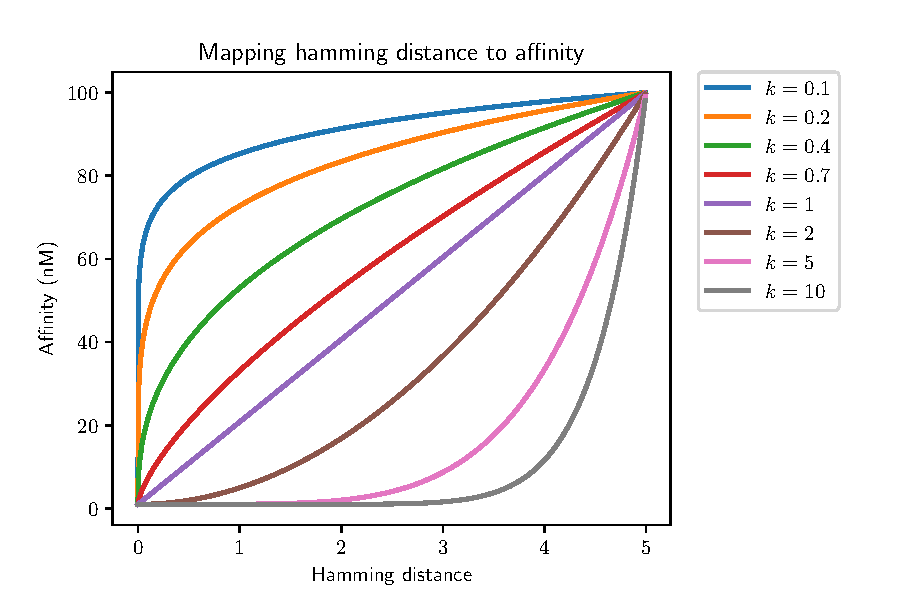
\includegraphics[width=0.8\textwidth]{figures/hd2affy.pdf}
    \caption{
        \label{fig:hd2affy}
        Varying the exponent $k$ in \eqref{eq:hd2affy} to achieve different mappings between distance and affinity. Naive -and mature affinity is held constant, $K^{\naive}_d = 100nM$ and $K^{\mature}_d = 1nM$.
    }
\end{figure}

It is easy to imagine that in a real affinity maturation process there will be many different BCR sequences that are practically equally fit.
E.g.\ this will happen when multiple amino acids are equally fit on a given position.
It will also happen if there are multiple distinct maturation paths that ends up with equally fit BCRs.
The later effect can be introduced into the model be adding more target sequences and then determining the affinity based on the shortest distance to all target sequences:
$$
d = \argmin_{\Tseq \in \Targets} \operatorname{dist}(\Bseq, \Tseq) 
$$






\subsubsection{Transforming BCR occupancy to fitness}
In the affinity model the fitness of a B cell is determined by the amount of antigen it binds relative to the total number of receptors it has, we shall call this $B^i_{\bound}$ for the BCR $B_i$.
The progeny distribution should adjust according to $B^i_{\bound}$, so if $B^i_{\bound}$ is small the progeny distribution should favor terminating the B cell and opposite, if $B^i_{\bound}$ is large this should cause the progeny distribution to favor cell division.
The Poisson distribution will reflect this behaviour by setting $\lambda_i$ small when $B^i_{\bound}$ is small and $\lambda_i$ large when $B^i_{\bound}$ is large.
To use $\operatorname{Pois}(\lambda_i)$ as the progeny distribution we need a function transforming $B^i_{\bound}$ to $\lambda_i$: $Y(B^i_{\bound}) = \lambda_i$.
For this purpose we can use a generalized version of the logistic function since this has the properties we need:
\begin{equation}
\lambda_i = Y(B^i_{\bound}) = \alpha \frac{K - \alpha}{G + Q \exp(-\beta B^i_{\bound})}
  \label{eq:BA_trans}
\end{equation}
$G$ is chosen to be the typical value of $1$.
$K$ is the upper bound of the function and is set to $2$, reflecting that the fastest average growth rate is $2^t$, with $t$ generations (setting $\operatorname{max}(\lambda) = 2$ is a model choice, but could be changed).
$\alpha$, $\beta$ and $Q$ are fit to fulfill three conditions:
\begin{equation}
Y(0) = 0, \ \ \ Y \left(\frac{f_{\full}}{U} \right) = 1, \ \ \ Y(f_{\full}) = 2 - \epsilon
  \label{eq:BA_cond}
\end{equation}
With $0 < f_{\full} \leq 1$ being the fraction of bound BCRs ($B^i_{\bound}$) that is sufficient to make the B cell close to fully activated.
Close in the sense that $Y(f_{\full})$ is close to the maximum $\lambda$ of 2, and therefore binding more antigen does not results in much change in the progeny distribution.
The constant $U$ in condition 2 can be adjusted to set the value of $B^i_{bound}$ resulting in $\lambda_i = 1$, and because $\frac{f_{\full}}{U} < f_{\full}$ we have that $U > 1$.
The interpretation of $U$ is that it is the fraction of BCRs binding antigen necessary to sustain the life of the B cell, but nothing more or less.
Using these conditions $\alpha$, $\beta$ and $Q$ can be found and the logistic function is fully defined.
$\alpha$ can be interpreted as the lower bound of the function and is therefore expected to be negative but close to 0, unless $U$ is large in which case $\alpha$ has to adjust accordingly to a large negative value, see figure \ref{fig:T_Bbound_U}.
$\beta$ is the growth rate, or steepness of the function, and it is coupled to the $Q$ parameter which will follow it according to the three conditions.
The steepness has to be high if saturation is reached a low $B^i_{bound}$ making $f_{\full}$ small, see figure \ref{fig:T_Bbound_f_full}.
\vfill

\begin{figure}
    \centering
    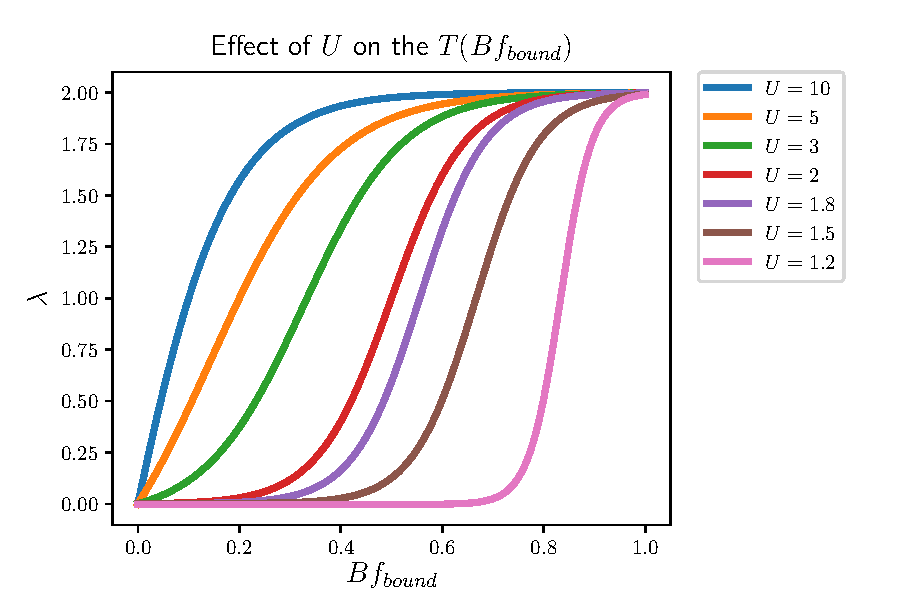
\includegraphics[width=0.8\textwidth]{figures/T_Bbound_U.pdf}
    \caption{
        \label{fig:T_Bbound_U}
        Using a constant $f_{\full} = 1$, changing the $U$ parameter in the conditions in equation \ref{eq:BA_cond} to achieve a shift of the inflection point, at $\lambda=1$, on the $B_{bound}$ axis.
    }
\end{figure}

\begin{figure}
    \centering
    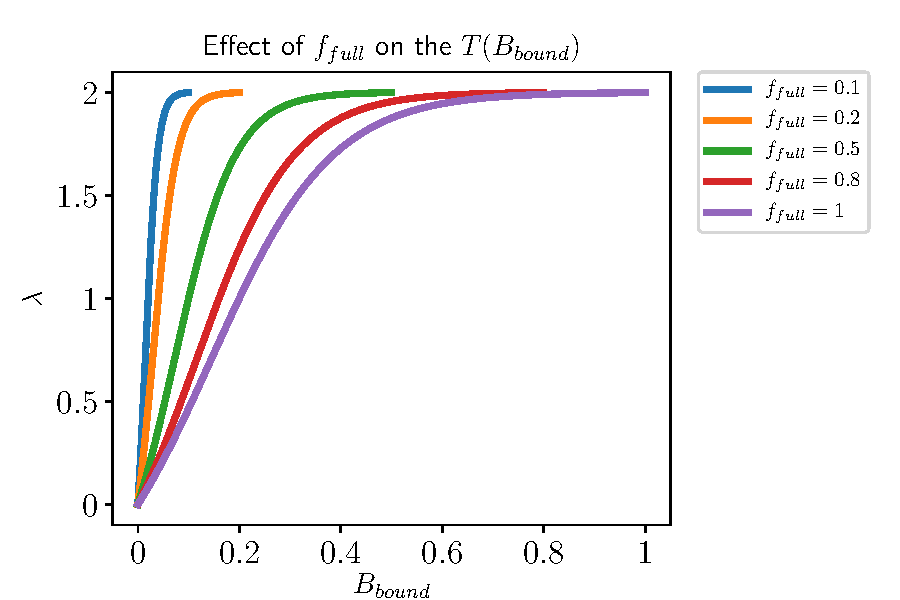
\includegraphics[width=0.8\textwidth]{figures/T_Bbound_f_full.pdf}
    \caption{
        \label{fig:T_Bbound_f_full}
        Using a constant $U = 5$, changing the $f_{\full}$ parameter in the conditions in equation \ref{eq:BA_cond} to change the point where $B_{bound}$ reaches the largest $\lambda$.
    }
\end{figure}








\subsubsection{The carrying capacity of a GC}
Finally we need to introduce the concept of a carrying capacity of a GC, which is defined as the number cells a GC is able to support in its micro environment.
The carrying capacity is determined mainly by the total concentration of antigen, since binding to antigen controls the progeny distribution.
BCR affinity is also influencing antigen binding, and therefore must influence the carrying capacity, but at high affinity nearly all antigen is bound, and hence the total antigen concentration is the most influential determinant of GC carrying capacity.
At $\operatorname{Pois}(1)$ the progeny distribution is only just sustaining the population size of the GC, and given from condition 2 in equation \ref{eq:BA_cond} this happens at $\frac{f_{\full}}{U}$.
Under the assumption that the population of B cells all have identical BCR sequences, the maximum carrying capacity is:
\begin{equation}
C([A_{\total}]) = U \frac{[A_{\total}] - [A]}{f_{\full}}
  \label{eq:carry_cap}
\end{equation}
The concentration of unbound antigen is determined by the affinity and concentration of BCRs.
It is fair to assume that there are many more BCRs than antigens, so for high affinity BCRs, the majority of antigen should be in a bound state allowing for the approximation of setting $[A]=0$.
This makes it easy to calculate the carrying capacity given equation \ref{eq:carry_cap}.
However in the cases with low affinity the concentration of free antigen cannot be assumed zero and in such cases $[A]$ can be determined through equation \ref{eq:A_objective}.

In the situation where a newly arising mutant has higher affinity than the rest of the population the fraction of BCR binding antigen on this mutant will approach $f_{\full}$, and in the case of $f_{\full} < 1$ it is even possibly surpasses it.
In these cases there is a probability that the clone will expand rapidly to overtake the GC population, also known as a clonal burst.
The clonal burst has the characteristic time (average time of take over) being:
$$
T_{\burst} = log_\kappa \left(carrying\ capacity \right) = log_\kappa\left( U \frac{[A_{\total}] - [A]}{f_{\full}} \right)
$$
With $\kappa = \operatorname{max}(\lambda)$ in this model fixed to 2 and $U$ and $f_{\full}$ being constants defined in the next section.






% \adcommentKD{This section will be supplemented by plots to justify the choice of parameters}

\subsection{Parameter choice}
%The choice of $f_{\full}$ determines the BCR occupancy when full activation of proliferation is achieved, but this interpretation is really just a simplification of the real biological system where multiple steps of interaction to both follicular dendritic cells and T cells are happening during the course of selection.
The choice of $f_{\full}$ determines the BCR occupancy when full activation of proliferation is achieved.
$f_{\full}$ does not have any known reference value so it is chosen to take a value of 1 because this is mathematically convenient.
It turns out that the model is quite robust to different choices of $f_{\full}$ and it causes no substantial effect to change it from 1 to 0.05, see figure \ref{fig:no_effect_of_f_full}.
Changing $f_{\full}$ will primarily effect the carrying capacity via. equation \ref{eq:carry_cap}, but by adjusting $[A_{\total}]$ to get the same carrying capacity simulations are indifferent to the choice of $f_{\full}$.
Presumably this is because the shape of the logistic transformation $Y(\cdot)$ in equation \ref{eq:BA_trans} will remain intact, see figure \ref{fig:T_Bbound_f_full}.
%Choosing a lower $f_{\full}$ will increase the carrying capacity but the shape of the logistic transformation $T$ will remain intact, see figure \ref{fig:T_Bbound_f_full}.
%We have chosen $f_{\full}$ to be $1$, with the interpretation that when half of the BCRs on a B cell are binding antigen it has a $\operatorname{Pois}(1)$ progeny distribution and when all BCRs are bound the progeny distribution increases to $\operatorname{Pois}(2-\epsilon)$.
The choice if $f_{\full} = 1$ has the interpretation that when half of the BCRs on a B cell are binding antigen it has a $\operatorname{Pois}(1)$ progeny distribution and when all BCRs are binding antigen, the progeny distribution increases to $\operatorname{Pois}(2-\epsilon)$.
\begin{figure}[!ht]
\begin{center}
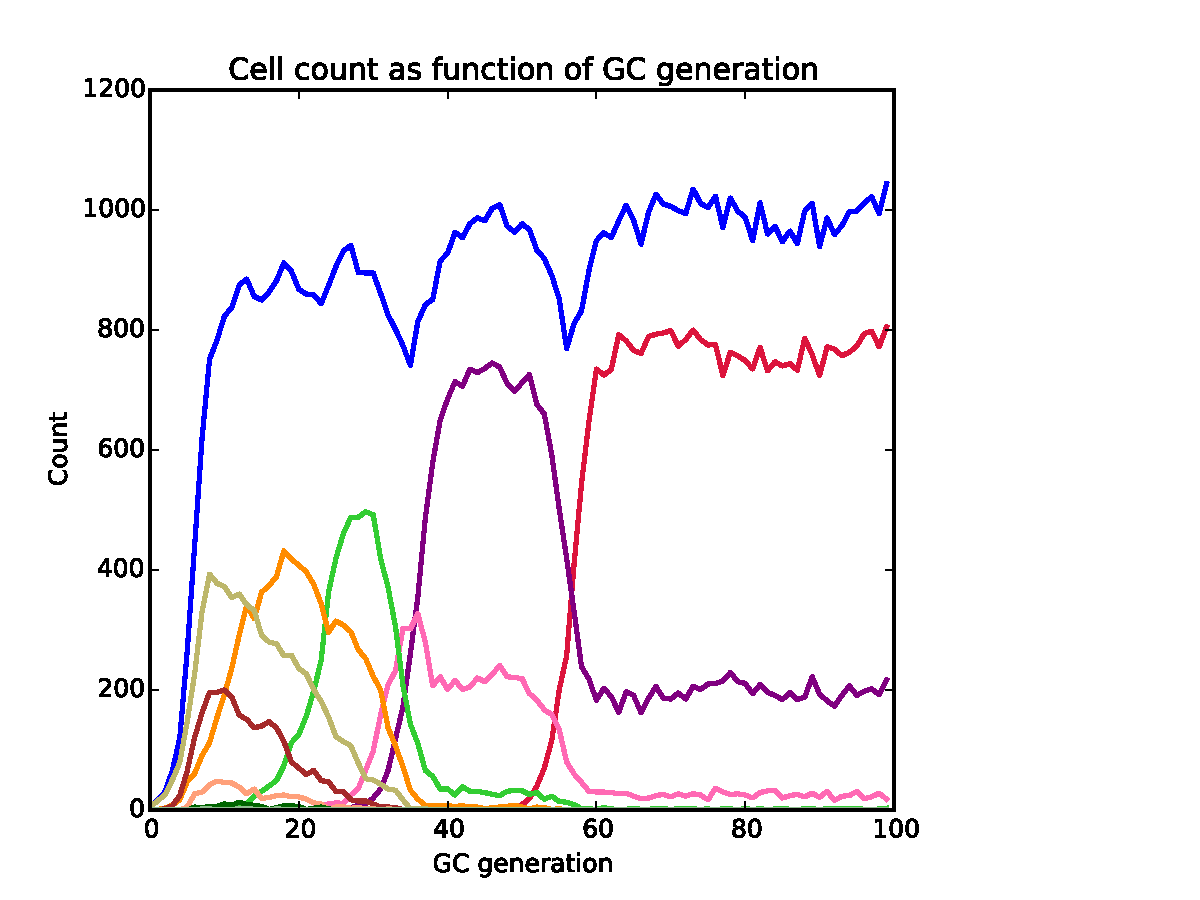
\includegraphics[height=49mm]{figures/f_full_1.pdf}
%\hspace{-40mm}
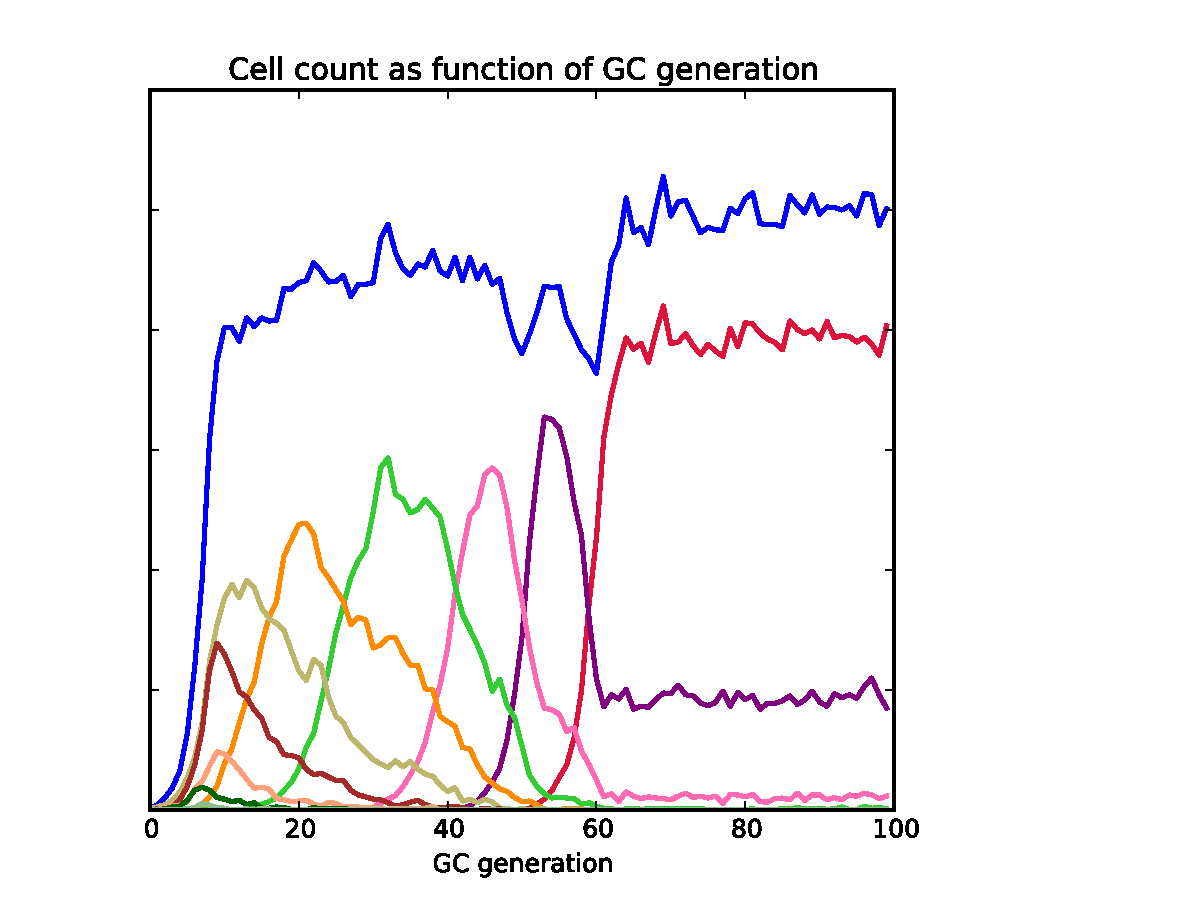
\includegraphics[height=49mm]{figures/f_full_05.pdf}
%\hspace{-40mm}
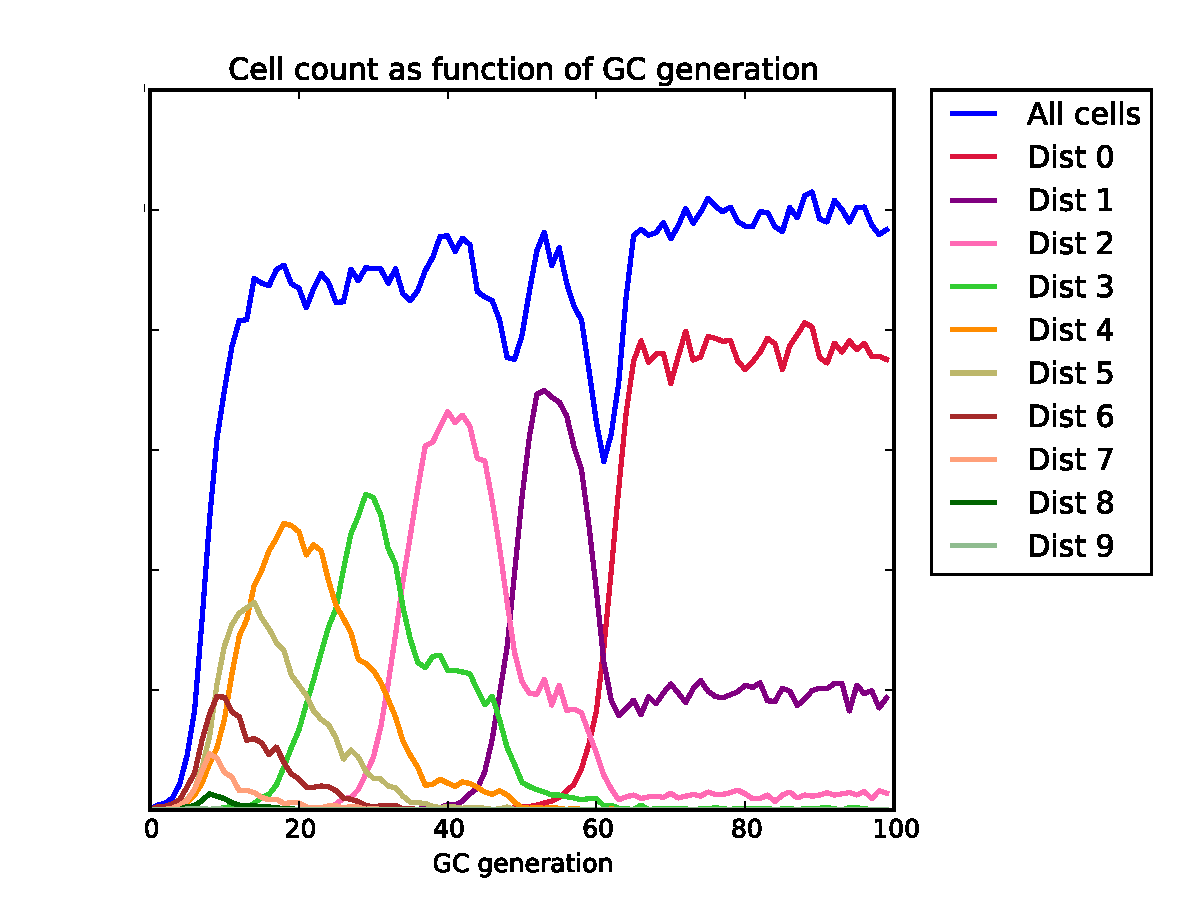
\includegraphics[height=49mm]{figures/f_full_005.pdf} \newline%
\end{center}
\vspace{-8mm} \hspace{23mm} (a) \hspace{37mm} (b) \hspace{37mm} (c)
    \caption{
        \label{fig:no_effect_of_f_full}
        Simulation with affinity selection for varying magnitudes of $f_{\full}$.
        $f_{\full}=1$, $f_{\full}=0.5$, $f_{\full}=0.05$ for (a), (b) and (c) respectively. Simulations with $U=5$ and $[A_{\total}]$ adjusted to obtain a carrying capacity of 1000 cells. Each simulation is run for 100 generations with $t_d=10$ and the composition of sequence distances to their closest targets are plotted for each generation.
        }
\end{figure}

We then chose the parameter $U$ in the logistic transformation to take a value to reflect our belief of how the shape of this transformation should look.
Our expectation is that initially, when only a few BCRs are bound and stimulation is low, there will be a linear increase of the stimulus with increasing antigen binding.
At some point close to $f_{\full}$, this increase in stimulus should level out because the cell can only be stimulated to $\operatorname{max}(\lambda)=2$.
This expected shape is recapitulated by a $U=5$, see figure \ref{fig:T_Bbound_U}, and therefore this is where we fix $U$.

In the transformation from distance to affinity in equation \ref{eq:hd2affy}, we have to make a choice about which exponent to use.
There is reason to believe that not all mutations are improving affinity with equal proportion and therefore the linear transformation is excluded.
Another thing we would like to enforce is to disallow sequences to drift far away from both the mature -and naive sequence.
A large sequence drift should not be very likely since it would complete abolish the binding of antigen.
For this reason it is preferred to have an exponent $k>1$.
We choose $k=2$ since this puts an extra penalty on simulated sequences that are drifting, without putting an excessive emphasis on the first two steps of approaching the mature sequence, see \ref{fig:hd2affy}.

The logistic function is chosen to yield a maximum $\lambda$ of 2 since this would correspond to an average max progeny of 2 cells yielding a population exponentially increasing by $2^t$, which is a standard exponential population growth.
%A $\operatorname{Pois}(2)$ progeny distribution is equal to saying that on average cells divide once per generation and that the total population is exponentially increasing by $2^t$, which is a standard exponential population growth.
One useful feature of the logistic function is that it has a notion of maximum signal i.e.\ when more antigen binding does not give more signal.
This flattening out is asymptotic approaching 2 which mean that the maximum growth rate of $\lambda=2$, is not reached completely at $f_{\full}$, so to fit the function we have to allow for this by choosing a small $\epsilon$ that make $Y(f_{\full})$ practically equivalent to 2.
Here we choose $\epsilon=\frac{1}{1000}$ meaning that $Y(f_{\full}) = \frac{1999}{1000}$.

Next we need to find some realistic numbers for the constants such as affinity, carrying capacity and $B^i_{\total}$.
First lets consider affinity.
$K_d$ for a naive sequence is likely in the low micro molar range range of $10^{-6} - 10^{-7} M$, while the mature affinity is in the nano -or subnano molar range of $10^{-8} - 10^{-10} M$ \cite{berek1987mutation}.
Classically these affinity measurements have been done using hapten induced immunizations, and there is reason to believe that conclusions about affinities will be different for other antigens.
Indeed it has been reported that naive sequences in some cases can be high affinity binders and affinity maturation is less useful \cite{frank2015simple}.
Nevertheless several groups have reported 50-100 fold affinity increase due to affinity maturation in both complex and hapten induced immunizations \cite{Kelsoe_2016}, \cite{phan2006high}, \cite{ulrich1997interplay}.
We choose the naive sequence to be $10^{-7} M$ ($100nM$) and the mature to be $10^{-9} M$ ($1nM$), giving a large span in affinity to select on.

With the introduction of $K_d$'s we need to consider units.
Lets start by estimating the concentration of BCRs per B cell in the GC, also denoted as $B^i_{\total}$.
To simplify things we assume that the number of BCRs on each B cell is the same.
In each GC there is an estimated $4 \times 10^3$ B cells \cite{kroese1990germinal}, but it has before been estimated to just $1000$ \cite{Childs_Baskerville_Cobey_2015} which we will use for convenience.
On the surface each of these B cells have an estimated $10^4$ BCRs \cite{rieckmann2017social}, \cite{immprot} (highly uncertain estimate), resulting in $10^7$ BCRs per GC.
Converting this to moles gives: $10^7\ 6 \times 10^{-23} moles$
The GC is reported to have a diameter of $10^{-4} m$ \cite{Romppanen_1981}.
Assuming the shape is spherical and converting to liters gives:
$$
\frac{4}{3} \pi (\frac{1}{2} \times 10^{-4} m)^3 10^3 \frac{L}{m^3} = \frac{1}{6} \pi \times 10^{-9} L
$$
Finally this gives:
$$\frac{10^7\ 6 \times 10^{-23} moles}{\frac{1}{6} \pi 10^{-9} L} \approx 10^{-6} M \equiv 10^{3} nM
$$
This means that each B cell contribute with approximately $1nM$ to the total concentration of BCRs.
Now to simplify things, everything is normalized to nano molar so e.g.\ the naive/mature affinity is changed to $100nM$ and $1nM$ respectively.
All the above described values are tabulated in table \ref{constants} and used as constant in later simulations of sequences undergoing affinity selection.

%We then make the assumption that the total concentration of antigen is equal to half of the total amount of BCRs in a fully grown GC with $10^3$ B cells each having $10^4$ BCRs.
%This makes a convenient reference point which is not unrealistic and we shall see later that the outcome of the simulations are rather insensitive to the concentration of antigens over a certain threshold.
%By looking at the definition of $[AB_n]$ it can be seen that changing the total concentration of antigen has the same effect as shifting the affinity of both the naive -and mature sequence by the same fraction and this is the way it can easily be investigated.
%   - With the side effect of increasing the carrying capacity.


\begin{table}[ht]
\centering
\begin{tabular}{llll}
Constant    & Value & Description & Reference \\ \hline
$B^i_{\total}$ & $1\times10^{4}$     & Number of BCRs on each B cell & \cite{immprot}, \cite{rieckmann2017social}*     \\
$n_t$ & 1000 & B cells per GC &  \cite{kroese1990germinal}, \cite{Childs_Baskerville_Cobey_2015} \\
d & $10^{-4} m$ & GC diameter &  \cite{Romppanen_1981} \\
U           & 5     & Fraction BCR bound necessary to sustain population & See text \\
k           & 2     & Exponent of affinity transformation & See text  \\
$f_{\full}$  & 1     & Fraction BCR bound at full response & See text \\
$K_d^{\naive}$ & 100nM & Naive affinity & \cite{berek1987mutation} \\
$K_d^{\mature}$ & 1nM & Mature affinity & \cite{berek1987mutation} \\
\end{tabular}
\caption{
\label{constants}
    Constants used in the model of affinity selection. *There is a lot of uncertainty in this number and depending on the method it is estimated from $10^3$ to $10^7$.}
\end{table}









\subsection{Implementation}
In the solution to the BCR antigen binding equilibrium in \eqref{eq:A_objective} B cells having the same BCR sequence is included in the same $B^i_{\total}$, and the hence the $B^i_{\total}$ will be different when some B cell genotypes are highly abundant while others are less.
But now lets expand the index, $i$, to represent just a single B cell, resulting in the simplification that $[B^1_{\total}] = [B^2_{\total}] = \ldots = [B^i_{\total}]$.
%The index, $i$, has then changed from a BCR genotype index to a B cell index.
In this notation multiple B cells can have the same BCR sequence, but each will have their own index because they are associated with different B cells.
This simplifies book keeping because the BCR index is always the same as the B cell index.
The change does not affect the solution in \eqref{eq:A_objective}.
Now given some total concentration of antigen, $A_{\total}$, the solution to the concentration of free antigen at equilibrium, $[A]$, reduces to finding the real positive root of the polynomial in \eqref{eq:A_objective}.
Finding this root is easily be done using Newton's method, or by using a faster method like the Broyden–Fletcher–Goldfarb–Shanno (BFGS) algorithm \cite{shanno1985broyden}.
Once its quantity is found, we can obtain the concentration of bound antigen by plugging $[A]$ into \eqref{eq:ABi}.
Lastly $B_bound$ is converted to a progeny distribution parameter $\lambda$ by using \eqref{eq:BA_trans}.

All the above model definitions have the single purpose of adjusting the progeny distribution of a cell through $\lambda_i$ given some fitness function.
Under the neutral model this fitness function is constant resulting in the same $\lambda_i$ for all cells while in the affinity selection model $\lambda_i$ are updated to reflect B cell fitness in a GC reaction.
Practically the simulation of sequences can be thought of as a process of constructing a phylogenetic tree, see figure \ref{fig:tree_iteration}.
In each generation all non terminated leaves on the tree is sampled and an integer is drawn from each of their progeny distributions.
The leaf can then either terminate or have $1$ to $N \in \Z_+$ progeny cells.
If the leaf has progeny each will undergo their own mutation process following the S5F model and become leaves in the next generation.
One generation is define as one iteration through all the non terminated leaves on the tree and this is done in random order to avoid any bias.
Once every leaf has be evaluated this marks a new generation and the generation time is increased by one.
For an overview see figure figure \ref{fig:tree_iteration}.

\begin{figure}
    \centering
    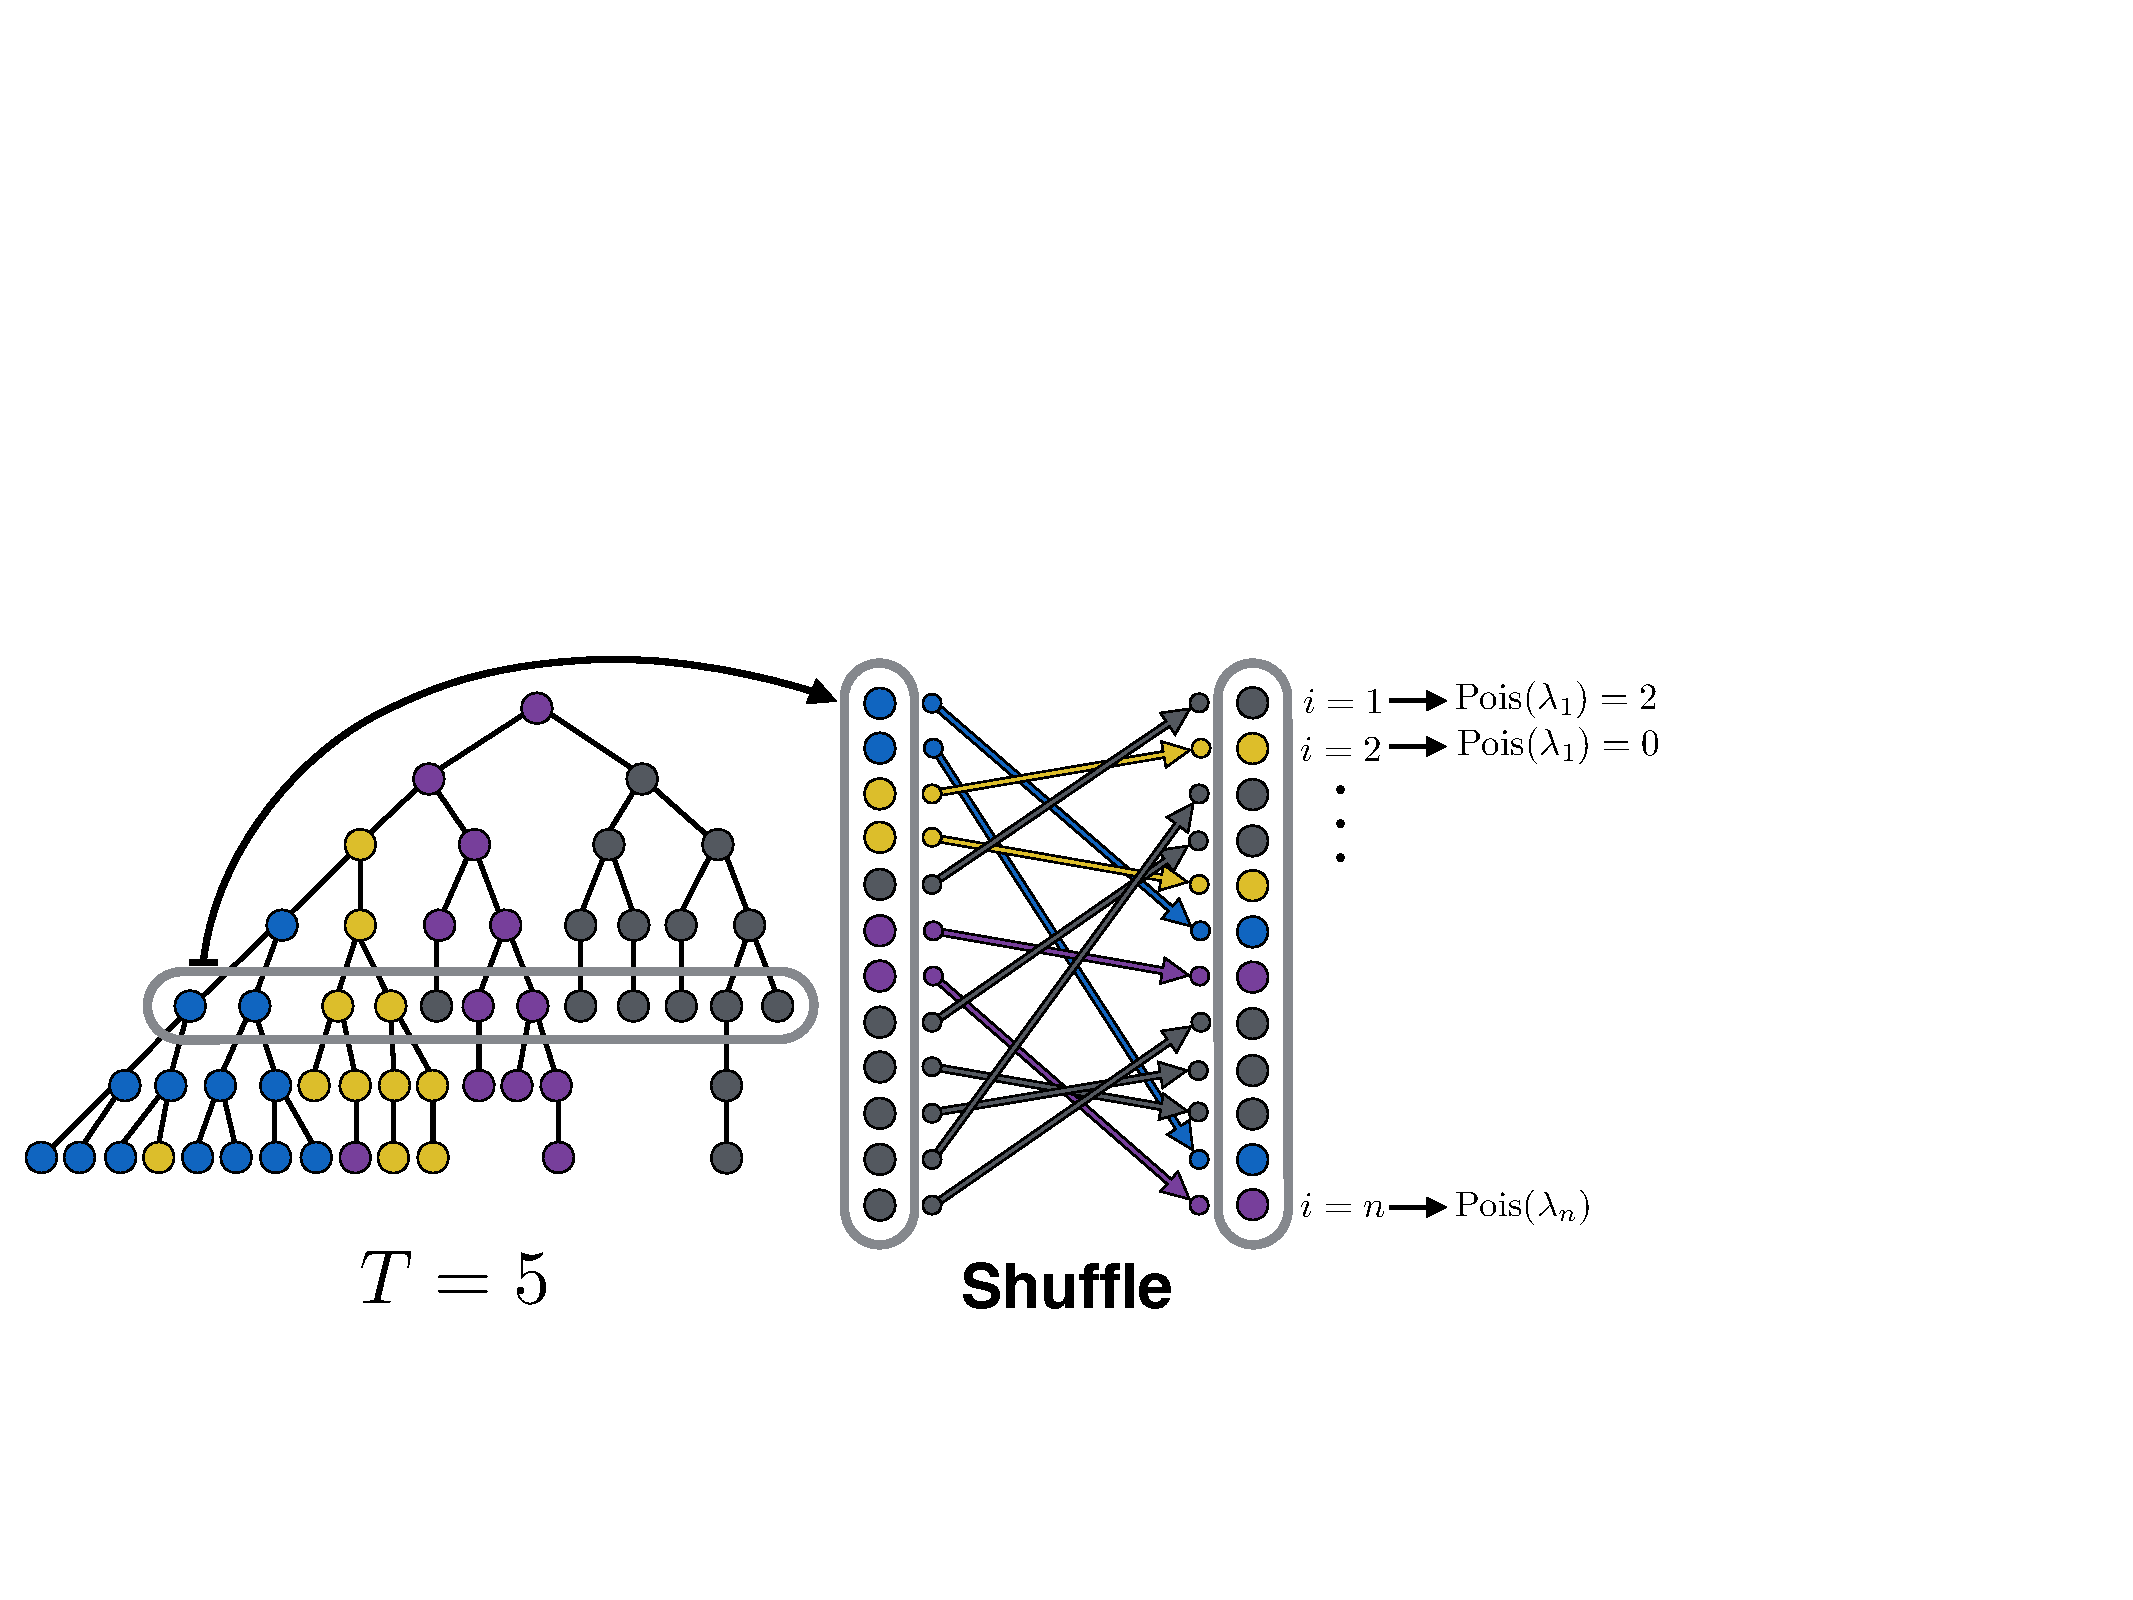
\includegraphics[width=1\textwidth]{figures/tree_iteration.pdf}
    \caption{
        \label{fig:tree_iteration}
        Illustration the sampling procedure in a time slice ($T=5$) of in the simulation of a phylogeny undergoing affinity selection.
        A generation time is defined as the time when all nodes have been sampled and their progeny have been evaluated.
        At each generation all non-terminated nodes will be evaluated in random order.
        For neutral selection $\lambda_i$ is constant and identical for all cells.
        For simulation with affinity selection $\lambda_i$ is B cell dependent and re-evaluated every time there is a change in the population of non-terminated nodes.
        This re-evaluation of all the $\lambda$s that can be skipped to for a number of nodes to save computation time without any substantial difference in simulation characteristics.
    }
\end{figure}


Using tree terminology the progeny distribution of a leaf depends on all the states (i.e.\ sequences) of the non terminated leaves.
Then by definition the affinity model needs to be updated, by re-evaluating equation \ref{eq:A_objective} and finding all $[AB]_i$, every single time a new leaf is generated, and the need for updating $[AB]_i$ will be a computational burden at large population sizes.
E.g.\ when simulating at a carrying capacity of 1000 cells, the vast majority of the computations are spent updating $[AB]_i$.
An approximate solution is simply to skip some of these updates and rely the previous determination of $\lambda_i$.
The rationale behind this is that when there is already a large population of cells, lets say 1000 non terminated leaves, then very little will change after a single leaf is evaluated.
In fact it turns out that for simulations using a carrying capacity of 1000 cells, there are no distinct difference between updating $[AB]_i$ after every leaf is evaluated or once every $\frac{1}{100}$th leaf evaluation, see figure \ref{fig:skip_vs_no_skip_dist10}.
\begin{figure}[!ht]
\begin{center}
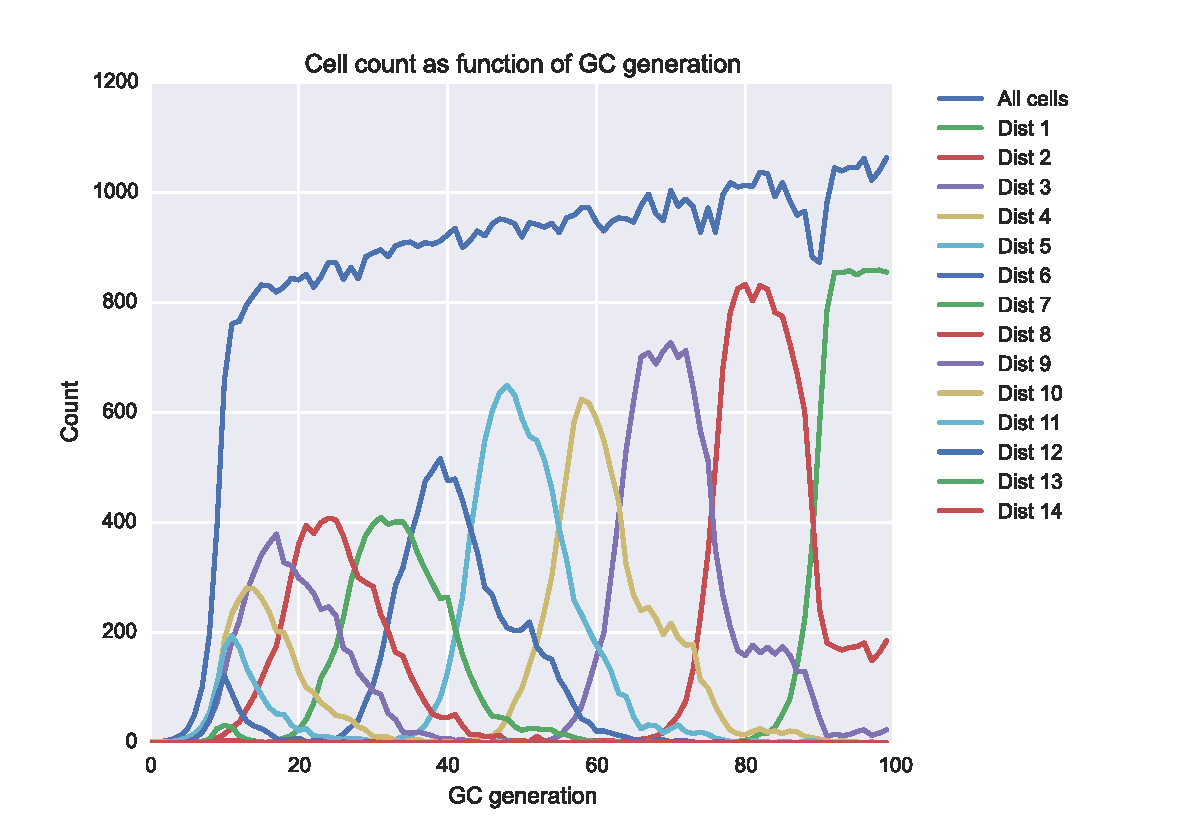
\includegraphics[width=80mm]{figures/sim_selection_default_run_dist10.pdf}
\hspace{-22mm}
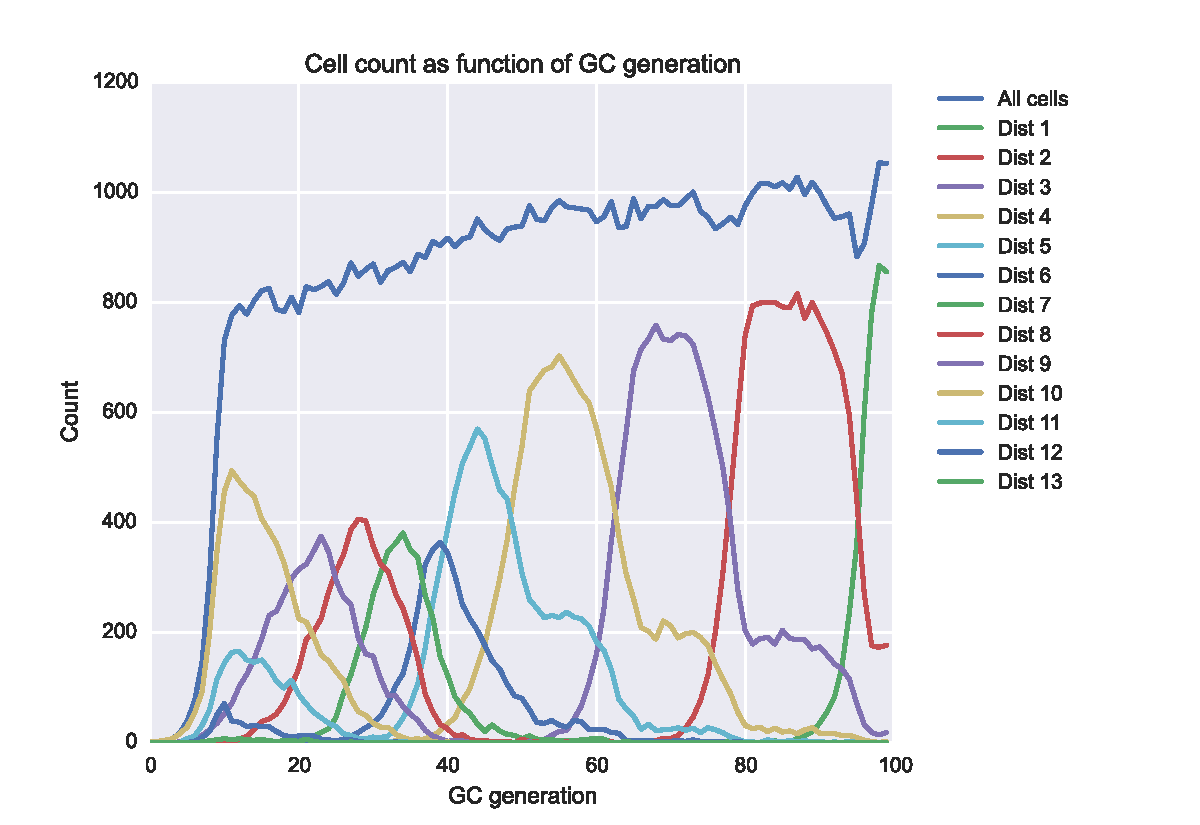
\includegraphics[width=80mm]{figures/sim_selection_default_run_dist10_no_skip.pdf} \newline%
\end{center}
\vspace{-9mm} \hspace{34mm} (a) \hspace{53mm} (b)
    \caption{
        \label{fig:skip_vs_no_skip_dist10}
        Simulation with selection comparing (a) with and (b) without skipping recalculation of $\lambda_i$ at each cell evaluation. In (a) no steps are skipped while, in (b), 99\% of all recalculations are skipped (10 updates to a population of 1000 B cells). Simulation parameters are default as in table \ref{aff_constants}, with $\lambda_0 = 0.3$ and $T=100$.
        }
\end{figure}

\iffalse
\begin{figure}[!ht]
\begin{center}
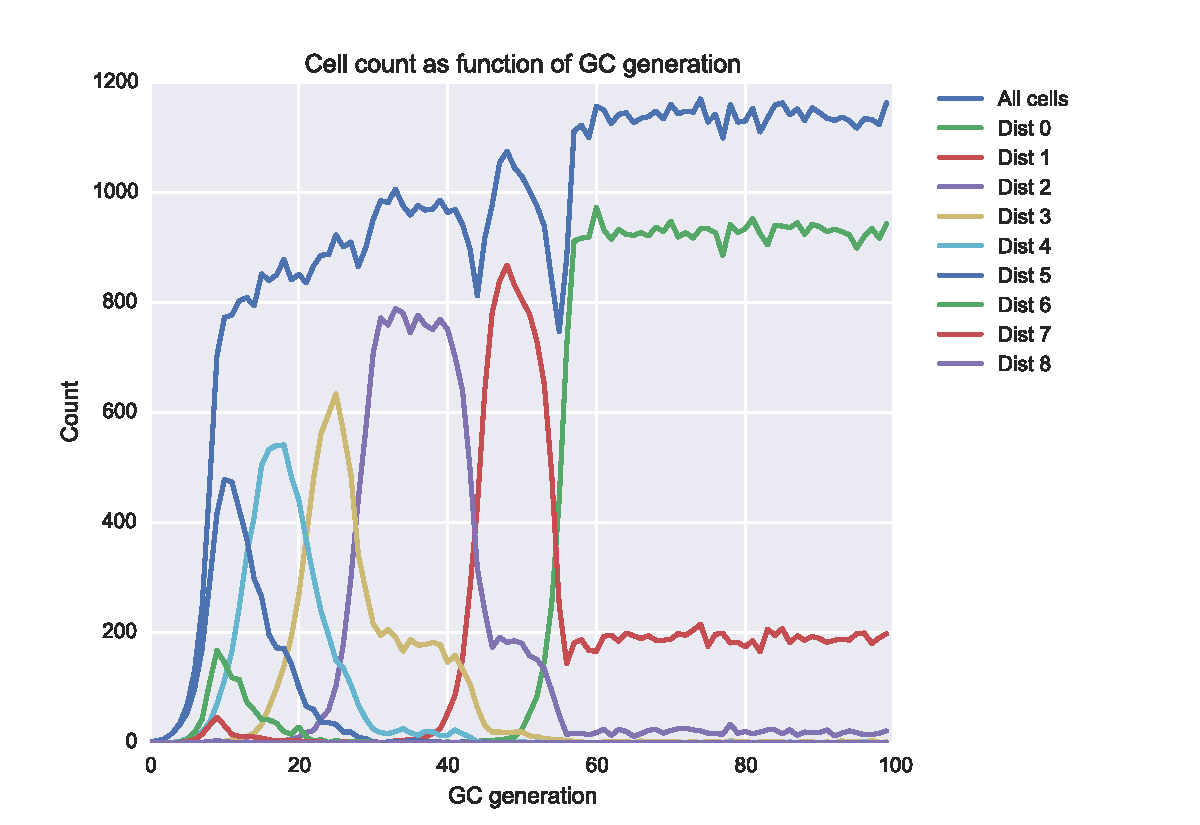
\includegraphics[width=80mm]{figures/sim_selection_default_run_dist5.pdf}
\hspace{-20mm}
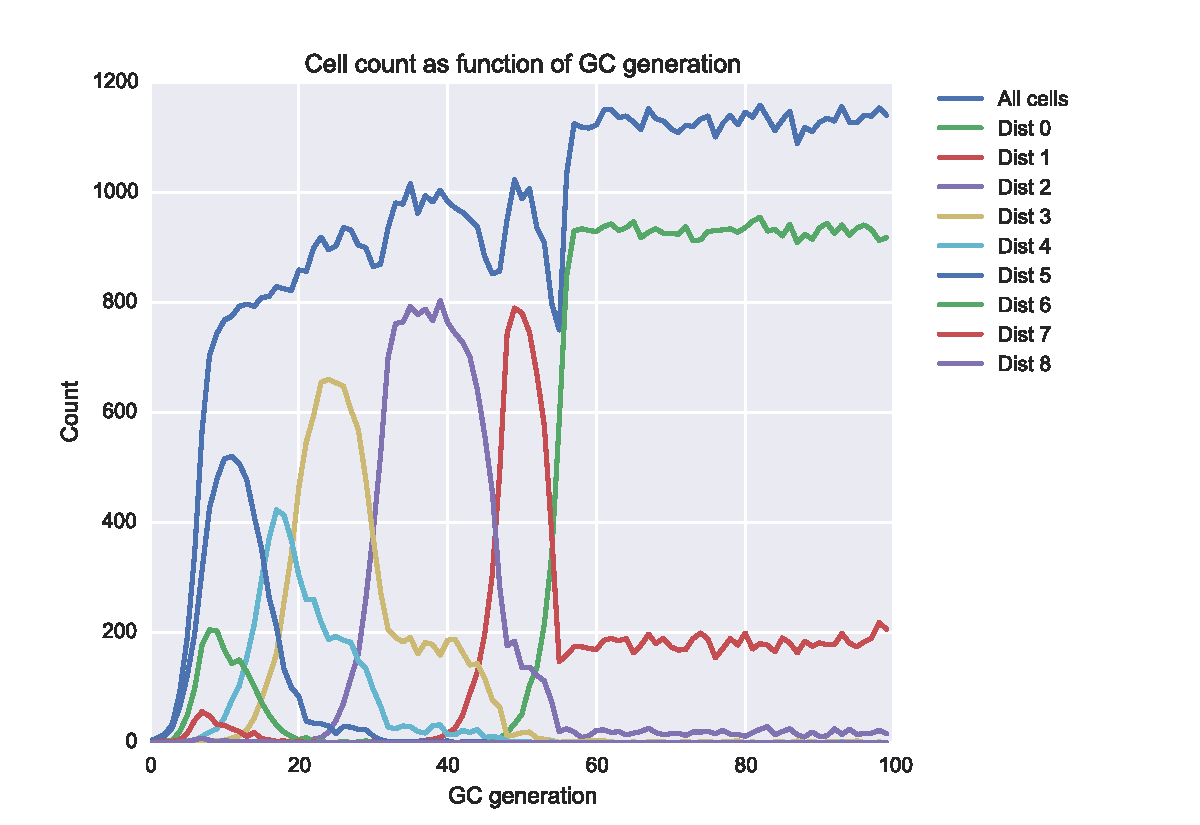
\includegraphics[width=80mm]{figures/sim_selection_default_run_dist5_no_skip.pdf} \newline%
\end{center}
\vspace{-9mm} \hspace{35mm} (a) \hspace{55mm} (b)
    \caption{
        \label{fig:skip_vs_no_skip_dist5}
        Simulation with selection comparing (a) with and (b) without skipping recalculation of $\lambda_i$ at each cell evaluation. In (a) no steps are skipped while, in (b), 99\% of all recalculations are skipped (ten updates to a population of a thousand B cells). In this simulation distance from naive to the mature sequence was 5 and $U$ was set to 2. The rest of the parameters are set to default parameters.
        }
\end{figure}
\fi


Target sequences ($\Tseq_i, i=1,2, \hdots, t_n$) can be arbitrarily defined by inputting a list of amino acid sequences.
Since affinity selection works on protein level the distance that determines affinity is the Hamming distance between two amino acid sequences.
Either one or multiple target sequences can be used but all are assumed to have equal affinity, $K^{\mature}_d$.
In the tests presented here we input the number of targets ($t_n$) and the amino acid distance from naive seed to target ($t_d$).
Using these parameters the target sequences are simulated by introducing DNA mutations into the naive sequence until it has diverged $t_d$ away from its starting point.
The mutations are introduced at DNA level given the neutral branching process described previously and thereby a distance of $t_d=10$ does not always correspond to 10 mutations, often the number is higher due to accumulation of synonymous mutations not counting towards protein level distance.
The process is repeated until $t_n$ targets have been made.
We reason that a good default choice of $t_d$, to achieve sufficient evolutionary distance, is 10, however the simulation behaviour seems rather indifferent to this, compare \ref{fig:no_effect_of_f_full} with \ref{fig:skip_vs_no_skip_dist10}.
The default number of targets ($t_d$) is set to 100 to provoke epistatic effects.
All default parameters in the affinity simulation is tabulated in table \ref{aff_constants}.
The implementation is available as a simulation subprogram in the codebase of \texttt{GCtree} (\url{github.com/matsengrp/gctree}).

\begin{table}[ht]
\centering
\begin{tabular}{lll}
Parameter    & Default & Description \\ \hline
$\lambda_0$ & None & $\operatorname{Pois}(\lambda_0)$ sequence mutability \\
$T$ & None & Stopping time \\
$cap$ & 1000 & Carrying capacity \\
$t_n$ & 100 & Number of random target sequence \\
$t_d$ & 10 & Distance from naive to target sequence \\
$n$ & all & Down-sampled number of sequence
\end{tabular}
\caption{
\label{aff_constants}
    Default parameters used in the affinity selected simulations.}
\end{table}










\subsubsection{The effect of having multiple mature targets}
%It is clearly easy to extend the affinity simulation with multiple target sequences serving as end point for maturation.
%%% More epistasis. It is already there before having multiple targets
% Since the affinity transformation is non-linear the effects of mutations are non-additive by definition.
By introducing multiple targets a side effect is that this introduces epistasis to the fitness landscape.
Epistasis is defined as non additive interaction between mutations and is widely observed in nature e.g.\ the evolution of influenza nucleoprotein \cite{gong2013stability}.
The manifestations of epistasis can be different, here is a simple example:
$$
ab = 1,\ Ab = 1,\ aB = 1,\ AB = 10
$$
There are four different genotypes, based on two loci (positions) with two alleles (gene variants), three having a fitness of 1 and one having a fitness of 10.
Each position is tolerable to the two states but only a combination of state $A$ and $B$ improves fitness.
In an linear additive, non epistatic, setting the effect of the intermediate states ($Ab$ and $aB$) should be measurable and sum to the effect of both:
$$
ab + (Ab - ab) + (aB -ab) = AB
$$
This is just one example of epistasis, where the effect is AND gate like.
The effect could also confer deleteriousness to the intermediate:
$$
ab = 1,\ Ab = \frac{1}{2},\ aB = \frac{1}{4},\ AB = 10
$$
Or any other non additive influence.

In the affinity simulation there is inherent epistasis because the transformation from distance to affinity is non-linear, although we could choose to fix $k=1$ in equation \ref{eq:hd2affy} to obtain linear additive distance effects.
Regardless, if simulation is done using multiple different targets it will be epistatic with multimodal fitness landscape as illustrated in figure \ref{fig:epistasis}.

\begin{figure}[!ht]
\begin{center}
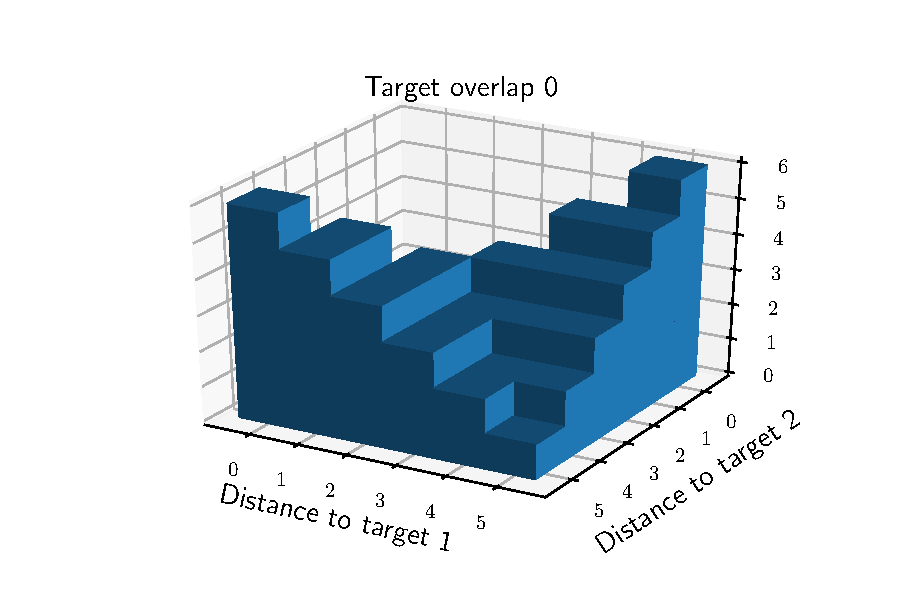
\includegraphics[height=35mm]{figures/fitness_overlap0.pdf}
%\hspace{-40mm}
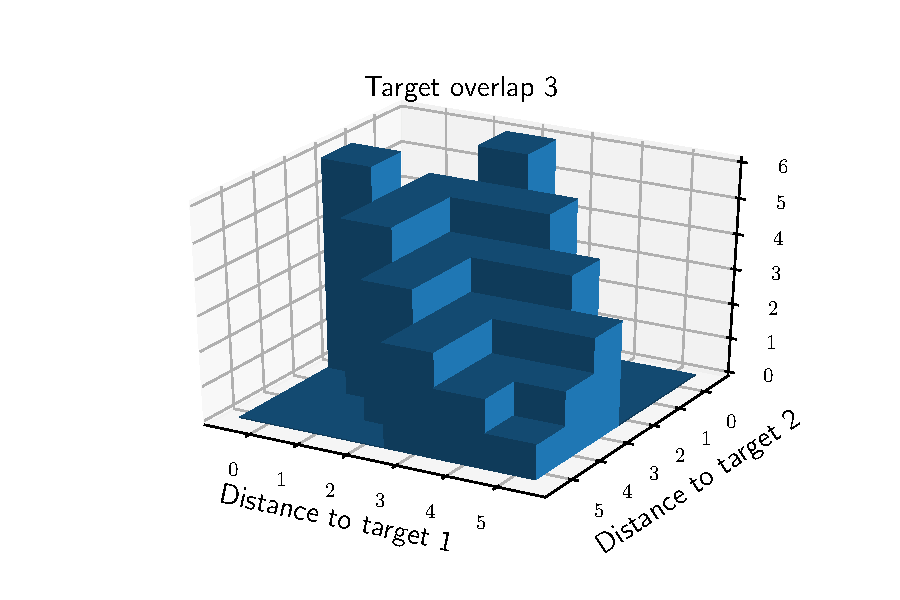
\includegraphics[height=35mm]{figures/fitness_overlap3.pdf}
%\hspace{-40mm}
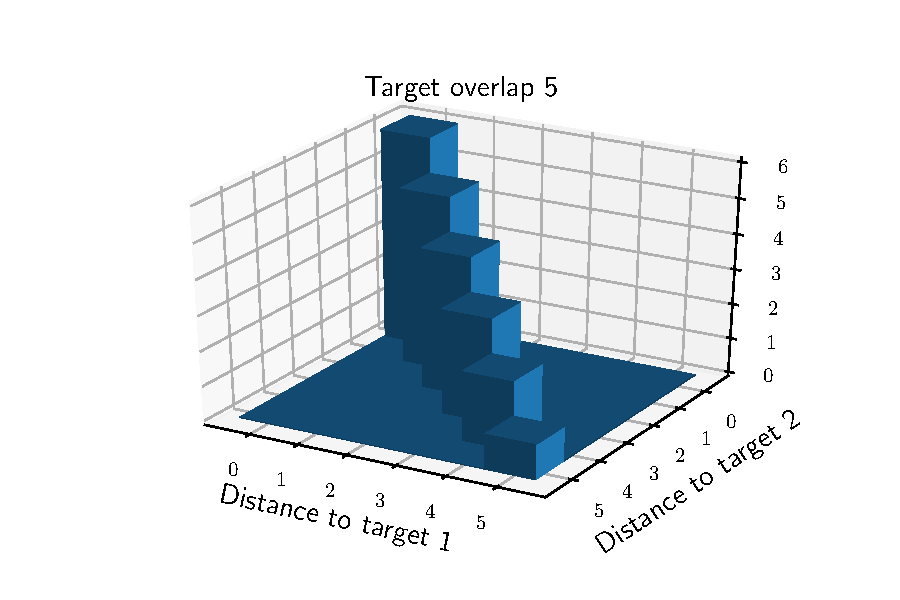
\includegraphics[height=35mm]{figures/fitness_overlap5.pdf} \newline%
\end{center}
\vspace{-6mm} \hspace{26mm} (a) \hspace{39mm} (b) \hspace{39mm} (c)
    \caption{
    \label{fig:epistasis}
        The effect of two target sequence on the fitness landscape.
        Two target sequences are created with varying overlap using $t_d=5$.
        The fitness landscape is constructed using a linear distance to affinity function ($k=1$ in equation \ref{eq:hd2affy}).
        In a) no overlap makes a long distance between the two peaks in fitness, in b) peaks are getting closer when targets overlap, and in c) when the overlap is complete the two targets match and the system no longer is epistatic.
        }
\end{figure}


Indeed the predictions of epistasis can be observed in simulation with multiple targets.
Often sequences are evolving towards a single target and once a few mutations have been accumulated a sequence is "committed" to this evolutionary trajectory.
However trajectories can change when a few mutation coincides with another target as observed in figure \ref{fig:epistasis_figure}.
These observations supports the view that the presented affinity simulation is a convoluted model being a good challenge to test the assumptions of inference methods.

\begin{figure}[!ht]
    \begin{center}
    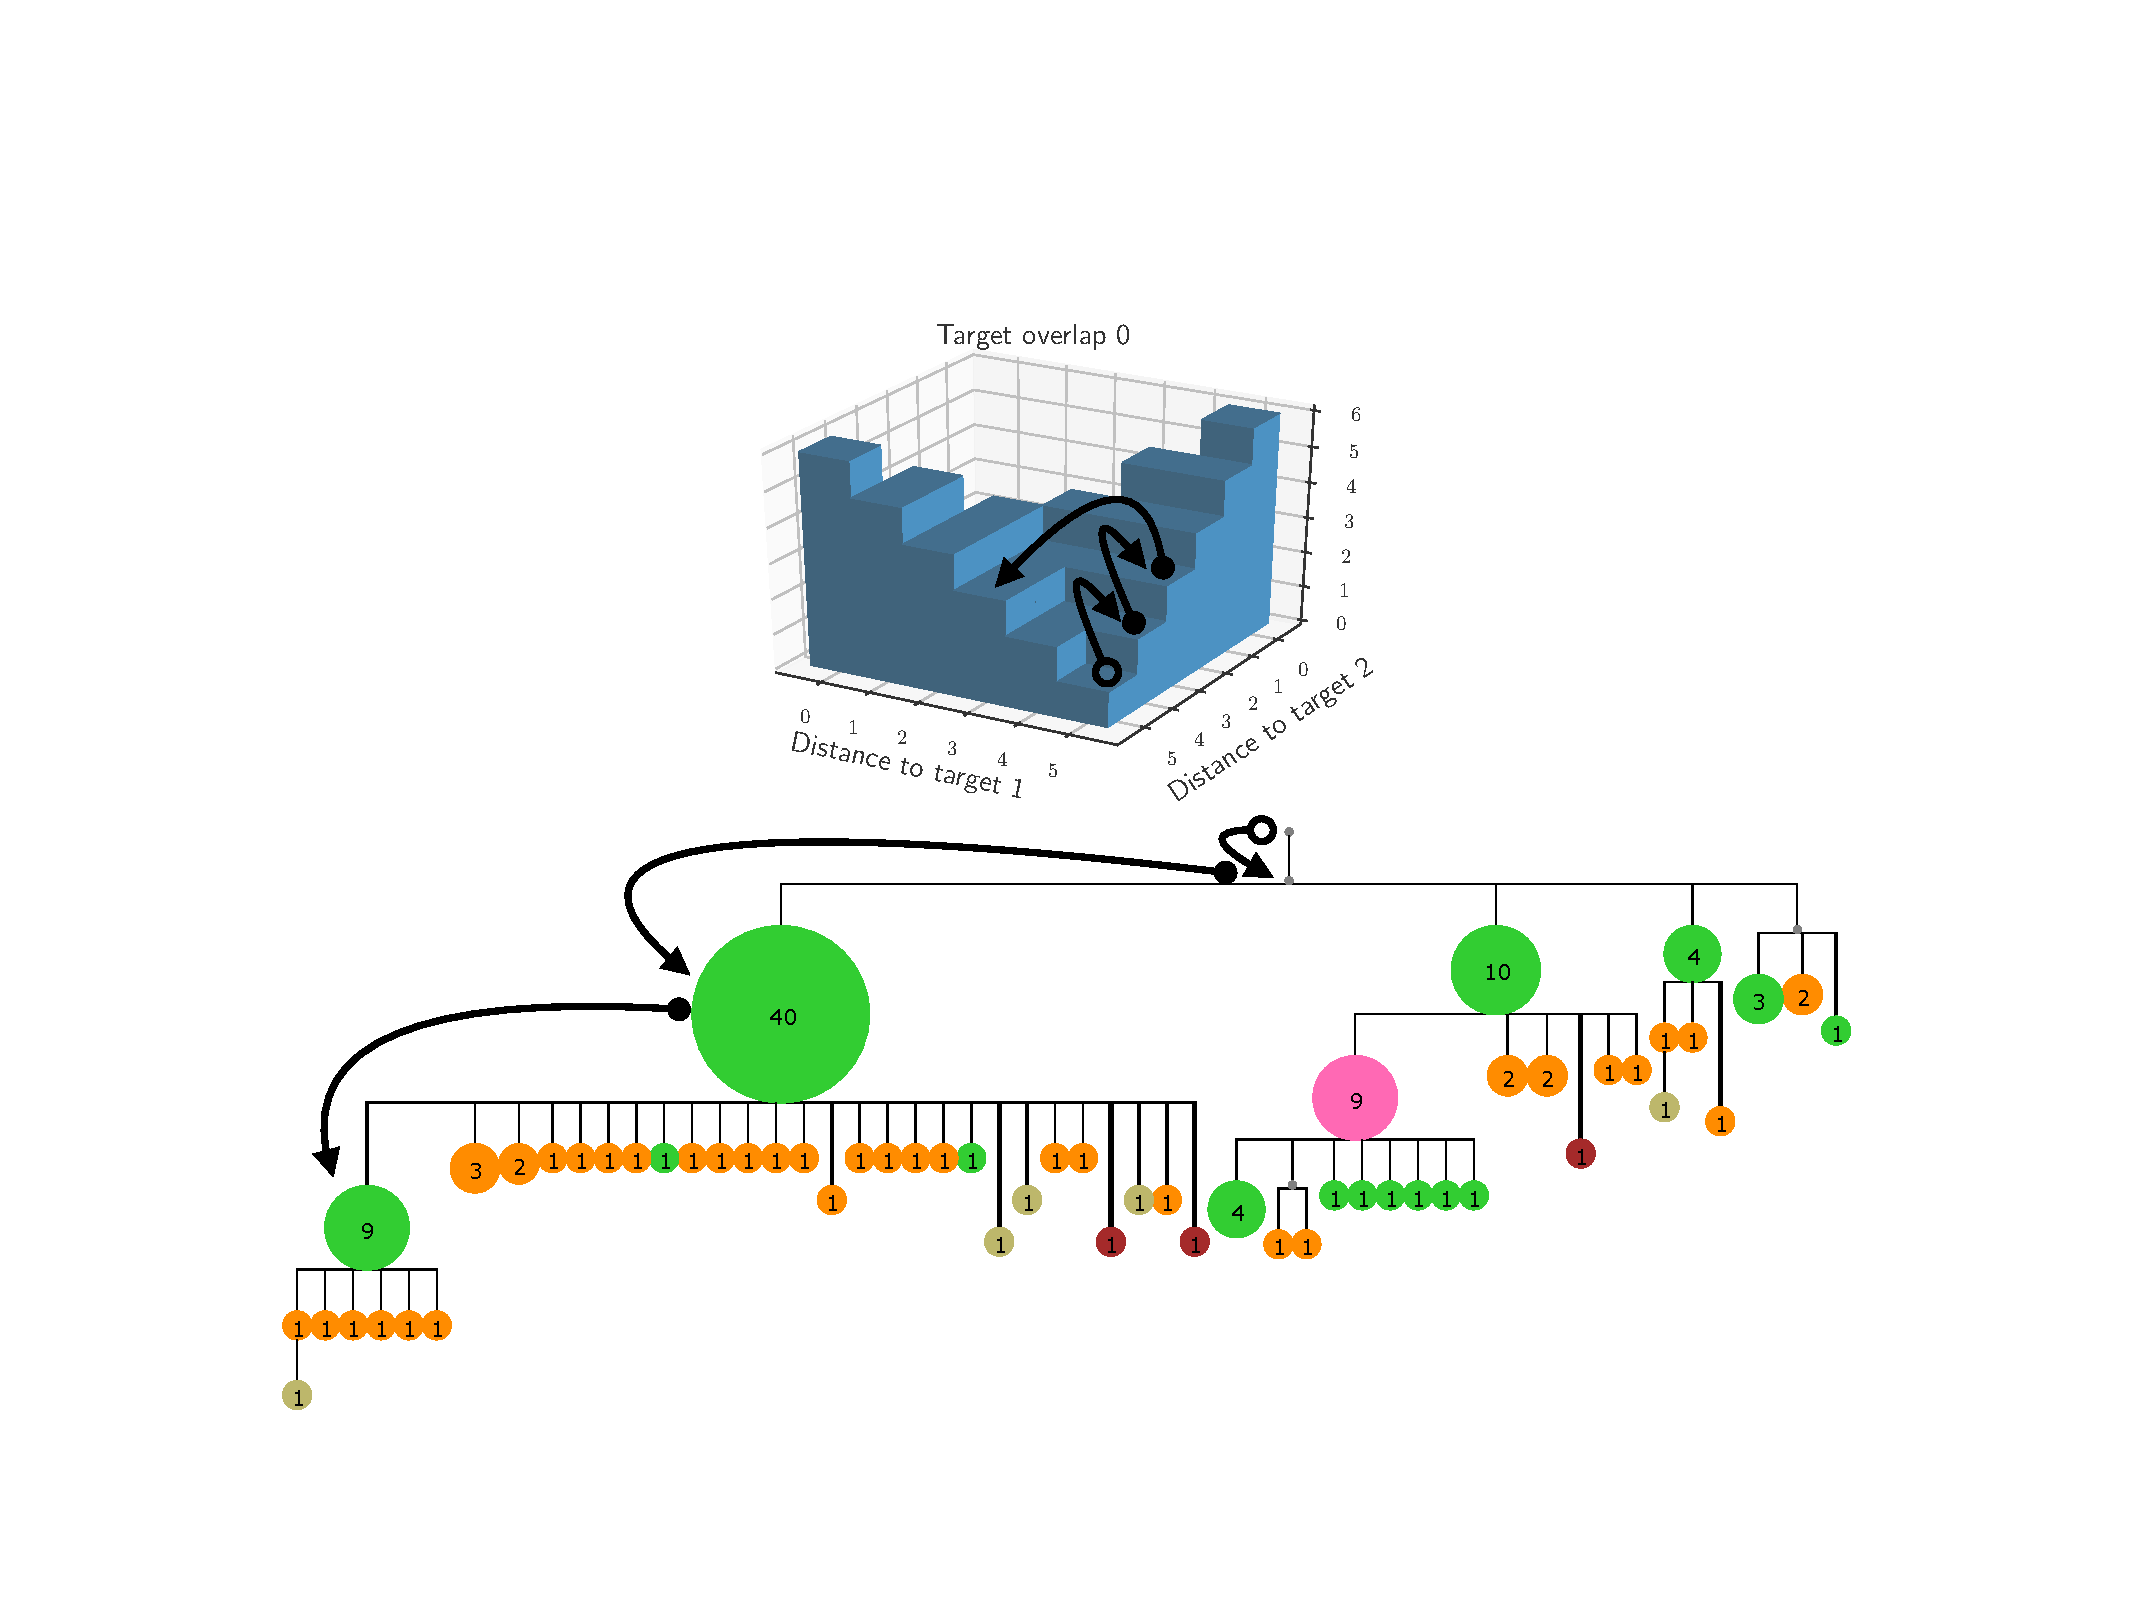
\includegraphics[width=0.8\textwidth]{figures/epistasis_figure.pdf}
        \caption{
        \label{fig:epistasis_figure}
        Example of epistasis in a simulation run with multiple target sequences.
        Colors correspond to the affinity of the simulated cells, see figure \ref{fig:collapsed_epistasis} in appendix B for run stats.
        Arrows show the evolutionary trajectory from lower levels in the fitness landscape to higher levels corresponding to root to tip on the phylogenetic tree, in both cases starting at the unfilled black circle.
        Zero amino acid distances leaves are collapsed and values inside nodes correspond to the number of B cells.
        Here we see that the simulation trajectory is following along several targets.
        There is even observed a jump between two target sequences trajectories, with the highest frequency node (green 40) yielding a decedent with two amino acid mutations (green 9) that is equally close to another target, resulting in a change in mutational trajectory.
        }
    \end{center}
\end{figure}








%\clearpage
\section{Results}
To test the simulation protocol and whether it recapitulates real world affinity maturation we needed a dataset with a known phylogeny starting from the naive sequence as a root node.
It is practically impossible to get such a dataset but something close was made by Tas et al. \cite{tas2016visualizing} with single cells sequencing of B cell isolated from the same GC.
The Tas. dataset consists of 65 BCR sequences.
Some sequences appear in multiple B cells and these are deduplicated and assigned abundances leaving a total of 42 different genotypes as observed in figure \ref{fig:Tas_tree}.
Reminding, that the phylogeny of the Tas. dataset is \textit{not} known but inferred based on a likelihood ranking of equally parsimonious trees (unpublished data).

\begin{figure}[!ht]
    \centering
    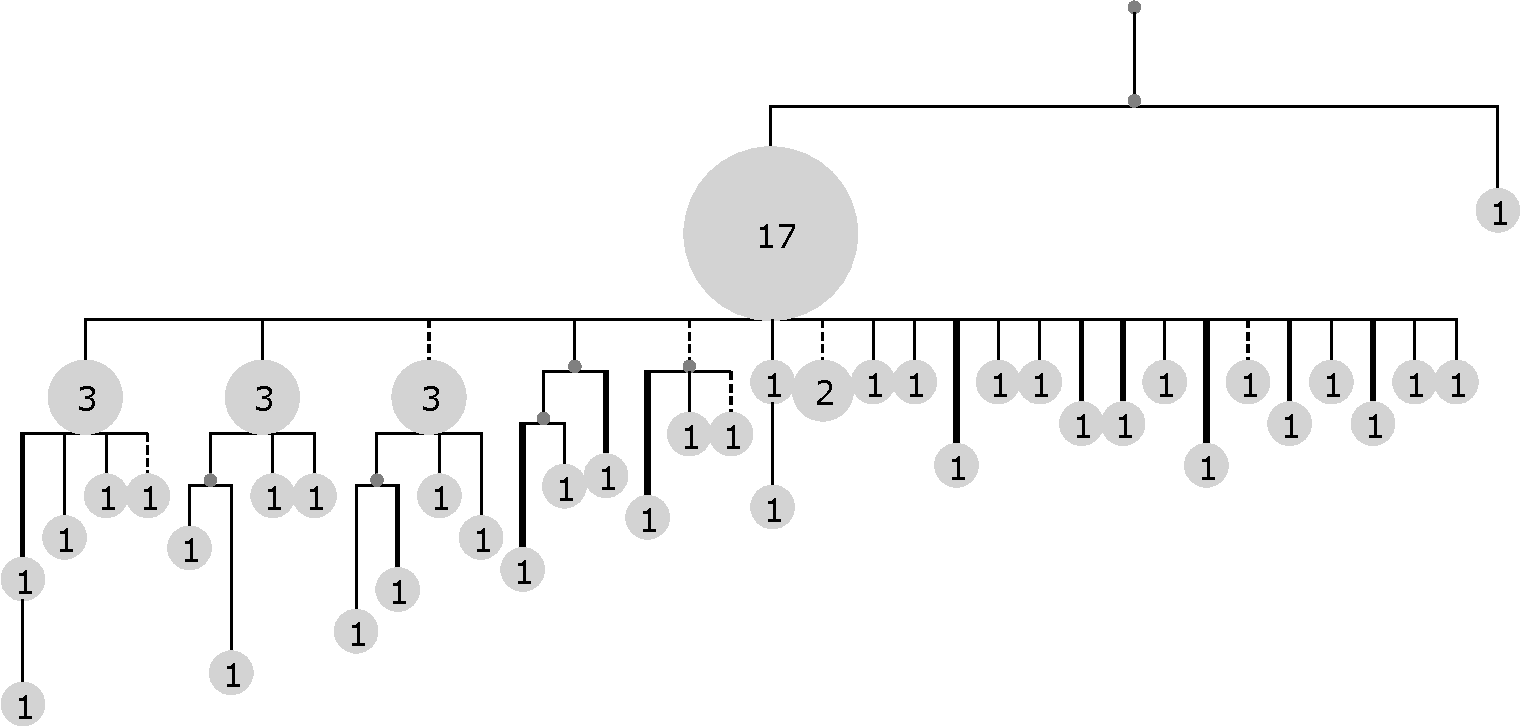
\includegraphics[width=0.8\textwidth]{figures/Tas_tree.pdf}
    \caption{
        \label{fig:Tas_tree}
        Inferred phylogeny for the single GC dataset from Tas et al. \cite{tas2016visualizing}.
        The inference method used is based on likelihood ranking of equally parsimonious trees, unpublished but implemented in the \texttt{GCtree} source code as a subprogram.
        Figure credit William S. DeWitt.
    }
\end{figure}


First we need a measure of accumulated SHM i.e.\ what is the percentage of mutations in the GC sequences and how is it distributed across the length of the tree.
We plot this mutation distribution as an empirical cumulative distribution function (CDF), see a) in figure \ref{fig:Tas-affsim_Tas-data}.
Next, genotype abundance is an important trait and indicator of clonal bursts.
Higher abundance clones are assumed to be more fit and should therefore also yield more offspring.
Some offspring will have a slightly different genotype with implication on fitness, hence high abundance clones should also have many different genotype descendents.
A proxy for counting these descendents is to count the immediate neighbors being just a single Hamming edit away, see b) in figure \ref{fig:Tas-affsim_Tas-data}.
If the assumption holds there should be a positive correlation between abundance and Hamming neighbors.

In figure \ref{fig:Tas-affsim_Tas-data} plotting the two above mentioned measures for the Tas. dataset, and superimposing the same measures but for 100 simulation runs, shows a consistent good fit between simulations and real data.
For this run parameters was set to $n=65$, $\lambda_0=0.25$, $t_d=5$, $T=35$ and default otherwise.
The down-sampling parameter ($n$) was set to the same number as sampled B cells in the Tas. dataset.
The seed naive sequence used was a V gene of 264 nt. and with the often referred SHM rate of $10^{-3}$ \cite{victora2012germinal} this gives $\lambda_0=0.264$ which was rounded to $\lambda_0=0.25$.
Target distance ($t_d$) and simulation time ($T$) was adjusted so the simulated sequences had approx. the same minimum Hamming distance to the naive sequence.

\begin{figure}
    \begin{center}
    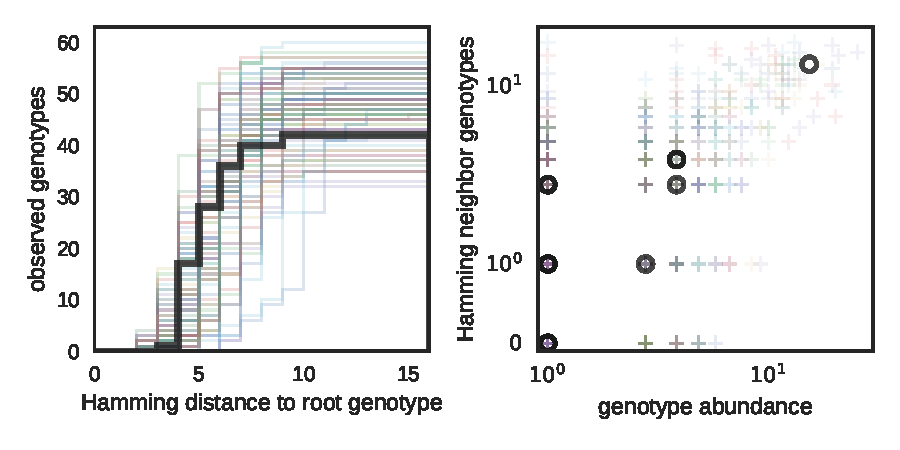
\includegraphics[width=0.8\textwidth]{figures/Tas-affsim_Tas-data.pdf}\newline%
    \end{center}
    \vspace{-14mm} \hspace{42mm} (a) \hspace{52mm} (b)
    \caption{
        \label{fig:Tas-affsim_Tas-data}
        Summary statistics for 100 simulations using $\lambda_0=0.25$, $t_d=5$, $T=35$ and $n=65$.
        Simulations are colored and Tas. dataset is black.
        In a) the cumulative distribution of mutations (empirical CDF) and b) the number of genotypes in 1 Hamming distance away as function of genotype abundance.
    }
\end{figure}


During affinity simulations the evolution of the cell population was plotted showing the emergence of new clones with higher affinity and their gradual take over of the cell population until an even more fit clone emerge, see appendix B figure \ref{fig:Tas_affsim_example_with_runstats}.
In all cases of affinity simulation there is a clear progression towards higher affinity as time passes until eventually a cell has reached the target sequence with highest affinity.
Topologically simulated trees also capture this notion of clonal bursts with one genotype suddenly being very dominant and yielding many offspring, see figure \ref{fig:Tas_affsim_example.collapsed_runstat_color_tree}.

\begin{figure}
    \centering
    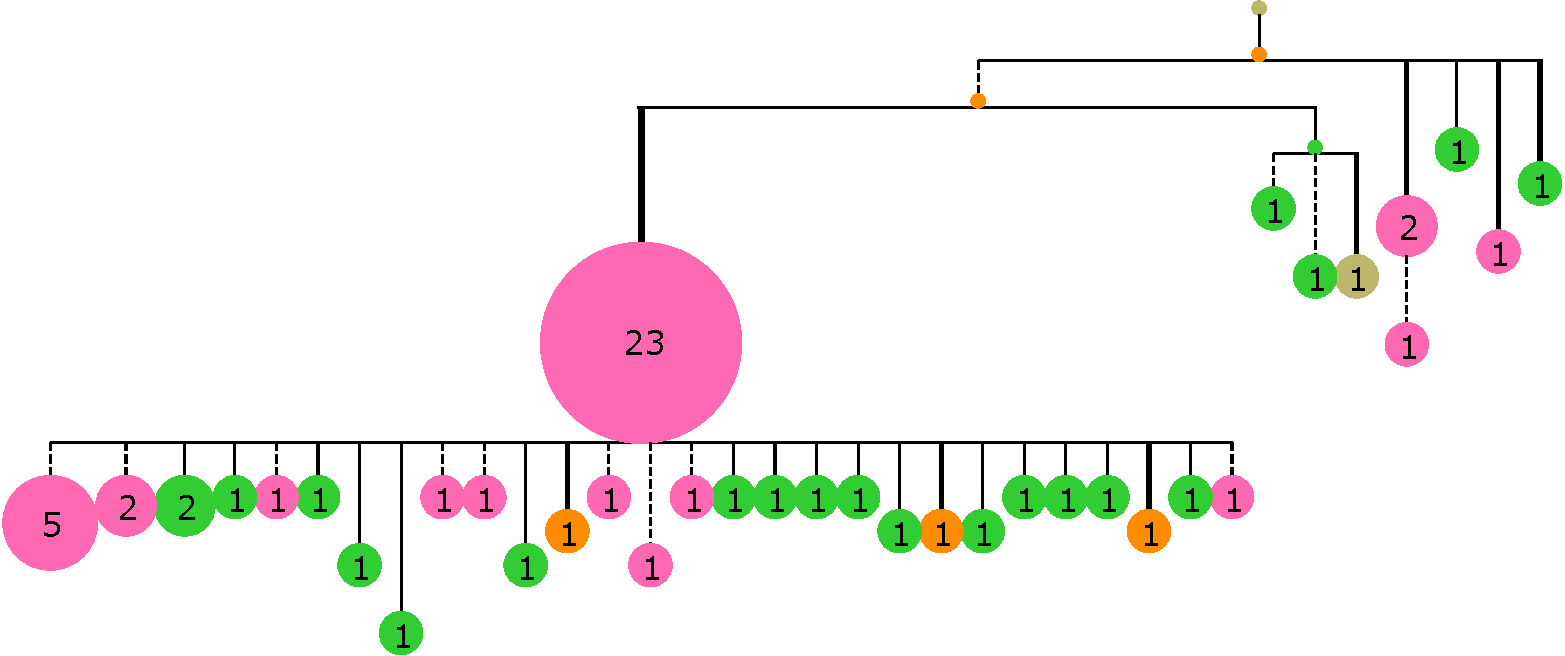
\includegraphics[width=0.8\textwidth]{figures/Tas_affsim_example_collapsed_runstat_color_tree.pdf}
    \caption{
        \label{fig:Tas_affsim_example.collapsed_runstat_color_tree}
        Simulated tree using $\lambda_0=0.25$, $t_d=5$, $T=35$ and $n=66$.
        For simulation statistics and color to affinity mapping see appendix B figure \ref{fig:Tas_affsim_example_with_runstats}.
    }
\end{figure}





%%% If doing another iteration of this model I would probably make the fitness a function of antigen bound relative to all the other cells instead of fraction BCRs binding antigen.
% Expressed in equations:
% fitness([AB_i]) = AB_i/sum(AB_i, i from 1 to N)
% In this way it would reflect T cell more realistically, but nevertheless the current model is already capturing most of this relative effect simply by binding more antigen when affinity is increased.
\section{Discussion and conclusion}
Previously many groups have made models of the GC reaction and affinity maturation \cite{Reshetova_2017}, \cite{Shahaf_2008}, \cite{Chaudhury_2014}, \cite{Wang_Mata_2015}, but none of these have included an explicit definition of the BCR sequences.
Neutral branching processes can easily be setup to simulation sequences undergoing the same mutational patterns as BCR sequences but they have no way of capturing the important clonal bursts happening due to the fitness gain from having a higher affinity BCR.
In this work we have addressed this problem through a simple but yet unexplored way of integrating affinity related fitness into the simulation of BCR sequence evolution.
A valuable tool in the assessment of inference methods.

It is interesting to see the similarities between the tree topologies of an affinity simulated tree compared to the inferred tree for the Tas. dataset.
As it was also noted in the work of Tas et al. \cite{tas2016visualizing} this GC has undergone a clonal burst with a clear dominant genotype (abundance 17 in figure \ref{fig:Tas_tree}) having many slightly mutated offspring.
Clearly this topological trait is very similar to the affinity simulated tree in figure \ref{fig:Tas_affsim_example_with_runstats}, and by mapping affinity to each node it can be seen that the clonal burst happened as a result of affinity gain
However as they also observed in Tas et al. appearance of a high affinity genotype does not guarantee a clonal burst, and as expected this is also true in the affinity simulation.
Under the best conditions a B cell has $\lambda=2$ from which it follows that $\operatorname{Pois}(termination | \lambda=2) = 0.135$, so there is roughly a 14\% chance of a high affinity clone turning extinct.


%The fitness function presented in this model is based on some rough assumptions about having a number of target sequences and using the distance from these as a proxy for affinity.
%However it is possible to plug in an arbitrary fitness function based on empirical values e.g.\ the affinity values determined from ancestral reconstruction of an antibody lineage like Doria-Rose et al. \cite{Doria-Rose2014-vi}.


The distribution of clones over time (e.g.\ see appendix B figure \ref{fig:Tas_affsim_example_with_runstats}) reveals that mutations conferring a fitness advantage are quickly found and fast at overtaking the whole cell population follows.
If this represents real affinity maturation it poses the problem that the probability of a maturation trajectory will be defined by the steepness of the fitness function and not the fitness at the end of a trajectory.
There is then a way of leading maturation into a dead end that is far lower in fitness than the global optimum but too high, compared to the naive state, to be reverted.
Indeed such a mechanism is a reasonable explanation why broadly neutralizing HIV antibodies are so rare.



\chapter{Ancestral sequence reconstruction of the B cell receptor phylogeny}

\section{Introduction}
With the wide availability and cost reductions of high throughput sequencing (HTS) it is getting commonly applied for studying the immune response through sequencing of the BCR and TCR repertoire.
Phylogenetic reconstruction of the evolution of the BCRs have recently gotten increasing attention because of its possible use in studying vaccine response.
There is a hope that with better understanding of the evolutionary trajectories of BCRs that the fate of the immune response can be modelled in a probabilistic framework, and that this will lead to new avenues in vaccine design finally addressing vaccination of HIV and broad influenza immunity.

By large the use of phylogenetics in BCR GC evolution has been made with the standard assumptions of site independence, constant mutation rates etc. using methods like maximum parsimony \cite{tas2016visualizing}, \cite{Barak2008-fw} and maximum likelihood \cite{Doria-Rose2014-vi}, \cite{Hoehn2016-wg}.
However we find that no study has yet investigated the validity of the phylogenetic assumptions in the context of BCR evolution.
It is important to note that most algorithms for phylogenetic inference have been made to study population genetics largely evolving under a neutrality or track the evolution of organisms over millions of years.
The consequences being that model assumptions are adjusted and validated in a completely different context than the highly selective, small population evolution that BCRs undergo in the GC reaction.
In contrast, BCR evolution has some interesting features that violates the assumption of classical phylogenetic methods e.g.\ the mutation model is DNA context sensitive, the root of the tree is known, high selection pressure on selected sites, sampled ancestors, very high mutation rates etc.

Validation studies are needed in order to understand weaknesses in the existing phylogenetic tool-chain, and opportunities to develop tools specific to the BCR case.
Sequence simulation is the cornerstone of all validation studies but unfortunately there has been no publicly available method for simulation of BCR sequence evolution.
Multiple articles have described simulations of VDJ recombined sequences \cite{safonova2015igsimulator}, \cite{ralph2016likelihood}, \cite{russ2015htjoinsolver} and few have also described simulation of B cell maturation \cite{shlomchik1998clone}, \cite{kleinstein2003estimating}.
Recombination centric simulations are usually not using a realistic model for simulating the SHM induced mutations in the GC reaction because their purpose is to test VDJ inference, and the few simulation programs emulating maturation are either closed source, does not model central parts of the GC reaction or entirely avoids dealing with sequences.
We are using a branching process, with and without selection, that is developed specifically for modelling the outcome of SHM in the GC reaction to test BCR lineage tree reconstruction under complex evolution.

In this paper we benchmark the performance of classical phylogenetic tools when applied to B cell receptor sequences, including tools for phylogenetic tree inference and for ancestral sequence reconstruction (ASR).
We do so in a realistic sequence simulation framework that can be used in the future for validating BCR specific methods as they develop.




\subsection{Ancestral sequence reconstruction}
When a phylogeny is inferred using a tree as a model for evolution, the tree will have internal nodes connecting the observations.
An internal state is also the inferred common ancestor of a number of leaves and/or branches and therefore sometimes referred to as an ancestral state.
All internal nodes are unknown, unobserved states, either explicitly defined by a sequence as in a parsimony tree, or defined by a likelihood function in model based phylogenies.
When a likelihood function is used to define internal states there is no longer a well defined ancestral sequence, instead this needs to be inferred as the maximum likelihood (ML) sequence estimate.
The ML estimate can be defined in two ways, as either marginal -or joint ML reconstruction.

In a marginal reconstruction the ML estimated sequence for one node is independent of the estimate of another i.e. $a_1 = \operatorname{max}(l(a_1 | t)), a_2 = \operatorname{max}(l(a_2 | t)), \hdots, a_n = \operatorname{max}(l(a_n | t))$, where $l$ is the likelihood function given a tree with branch length and data, $t$, and $a_i$ is an ancestral sequence on internal node $i$.
This makes it easy to find ancestral sequences by iterating through all internal nodes in arbitrary order.

Once an ancestral sequence has been fixed to an internal node this changes the likelihood function for the rest of the tree.
In fact all internal states are interdependent and while this is ignored in the marginal reconstruction it is taken into account in joint reconstruction by maximizing the likelihood of all ancestral states at once i.e. $a_1, a_2, \hdots, a_n = \operatorname{max}(l(a_1, a_2, \hdots, a_n | t)), a_2$.
It is a non trivial task to minimize this likelihood for many internal nodes, and though Pupko et al. \cite{pupko2000fast} showed how to speed up the joint reconstruction algorithm, most software is using the more simple marginal reconstruction.

While it is clear that joint reconstruction is the more probabilistically correct way of inferring ancestral sequences there is less clarity about whether or not this changes the estimated sequences.
The model based methods tested in this work are all using marginal reconstruction and therefore this will also be used in our validation.






\section{Methods}

\subsection{Measuring correctness of ancestral reconstruction}
In the following section we will introduce a benchmark metric for ancestral sequence reconstruction, we call this metric correctness of ancestral reconstruction (COAR).
The correctness of a reconstruction compared to the true evolutionary history can be measured by multiple similarity measures e.g.\ a) topological similarity, b) branch length similarity and c) sequence similarity between inferred and real ancestors.
All these measures are inter-dependent e.g.\ the inferred sequences are affected by the branch lengths and the topology and the branch lengths are determined given a topology etc.

Assume the loss function for ancestral sequence reconstruction is comprised of the three above mentioned terms.
The tree topology is the model framework of the phylogeny by which we can extract useful information like relatedness, ancestral sequences, distances and more.
In a model based phylogeny branch lengths are a measure for the expected number of substitutions per site so picking the correct branch lengths are important for reconstruction.
If the model underlying the phylogeny is a clock-model, where the branch lengths are related to evolutionary time, then the branch lengths are also interpretable, but otherwise interpretation is more difficult, and regardless of their magnitude, the branch lengths are merely numbers adjusted by the underlying phylogenetic model, and therefore the correctness of these are of secondary importance.
Lastly, the actual inferred ancestral sequences are determined by a combination of the underlying substitution model, the chosen tree and its branch lengths.
While inferring correct tree topology is also important, the correctness of the inferred ancestral sequences are the foremost important objective of a sequence reconstruction when these sequences are used for real applications involving DNA synthesis, protein expression and lab tests.
For this reason the sole purpose of the COAR metric is to capture the correctness of the inferred ancestral sequences.




\begin{figure}[ht!]
    \centering
    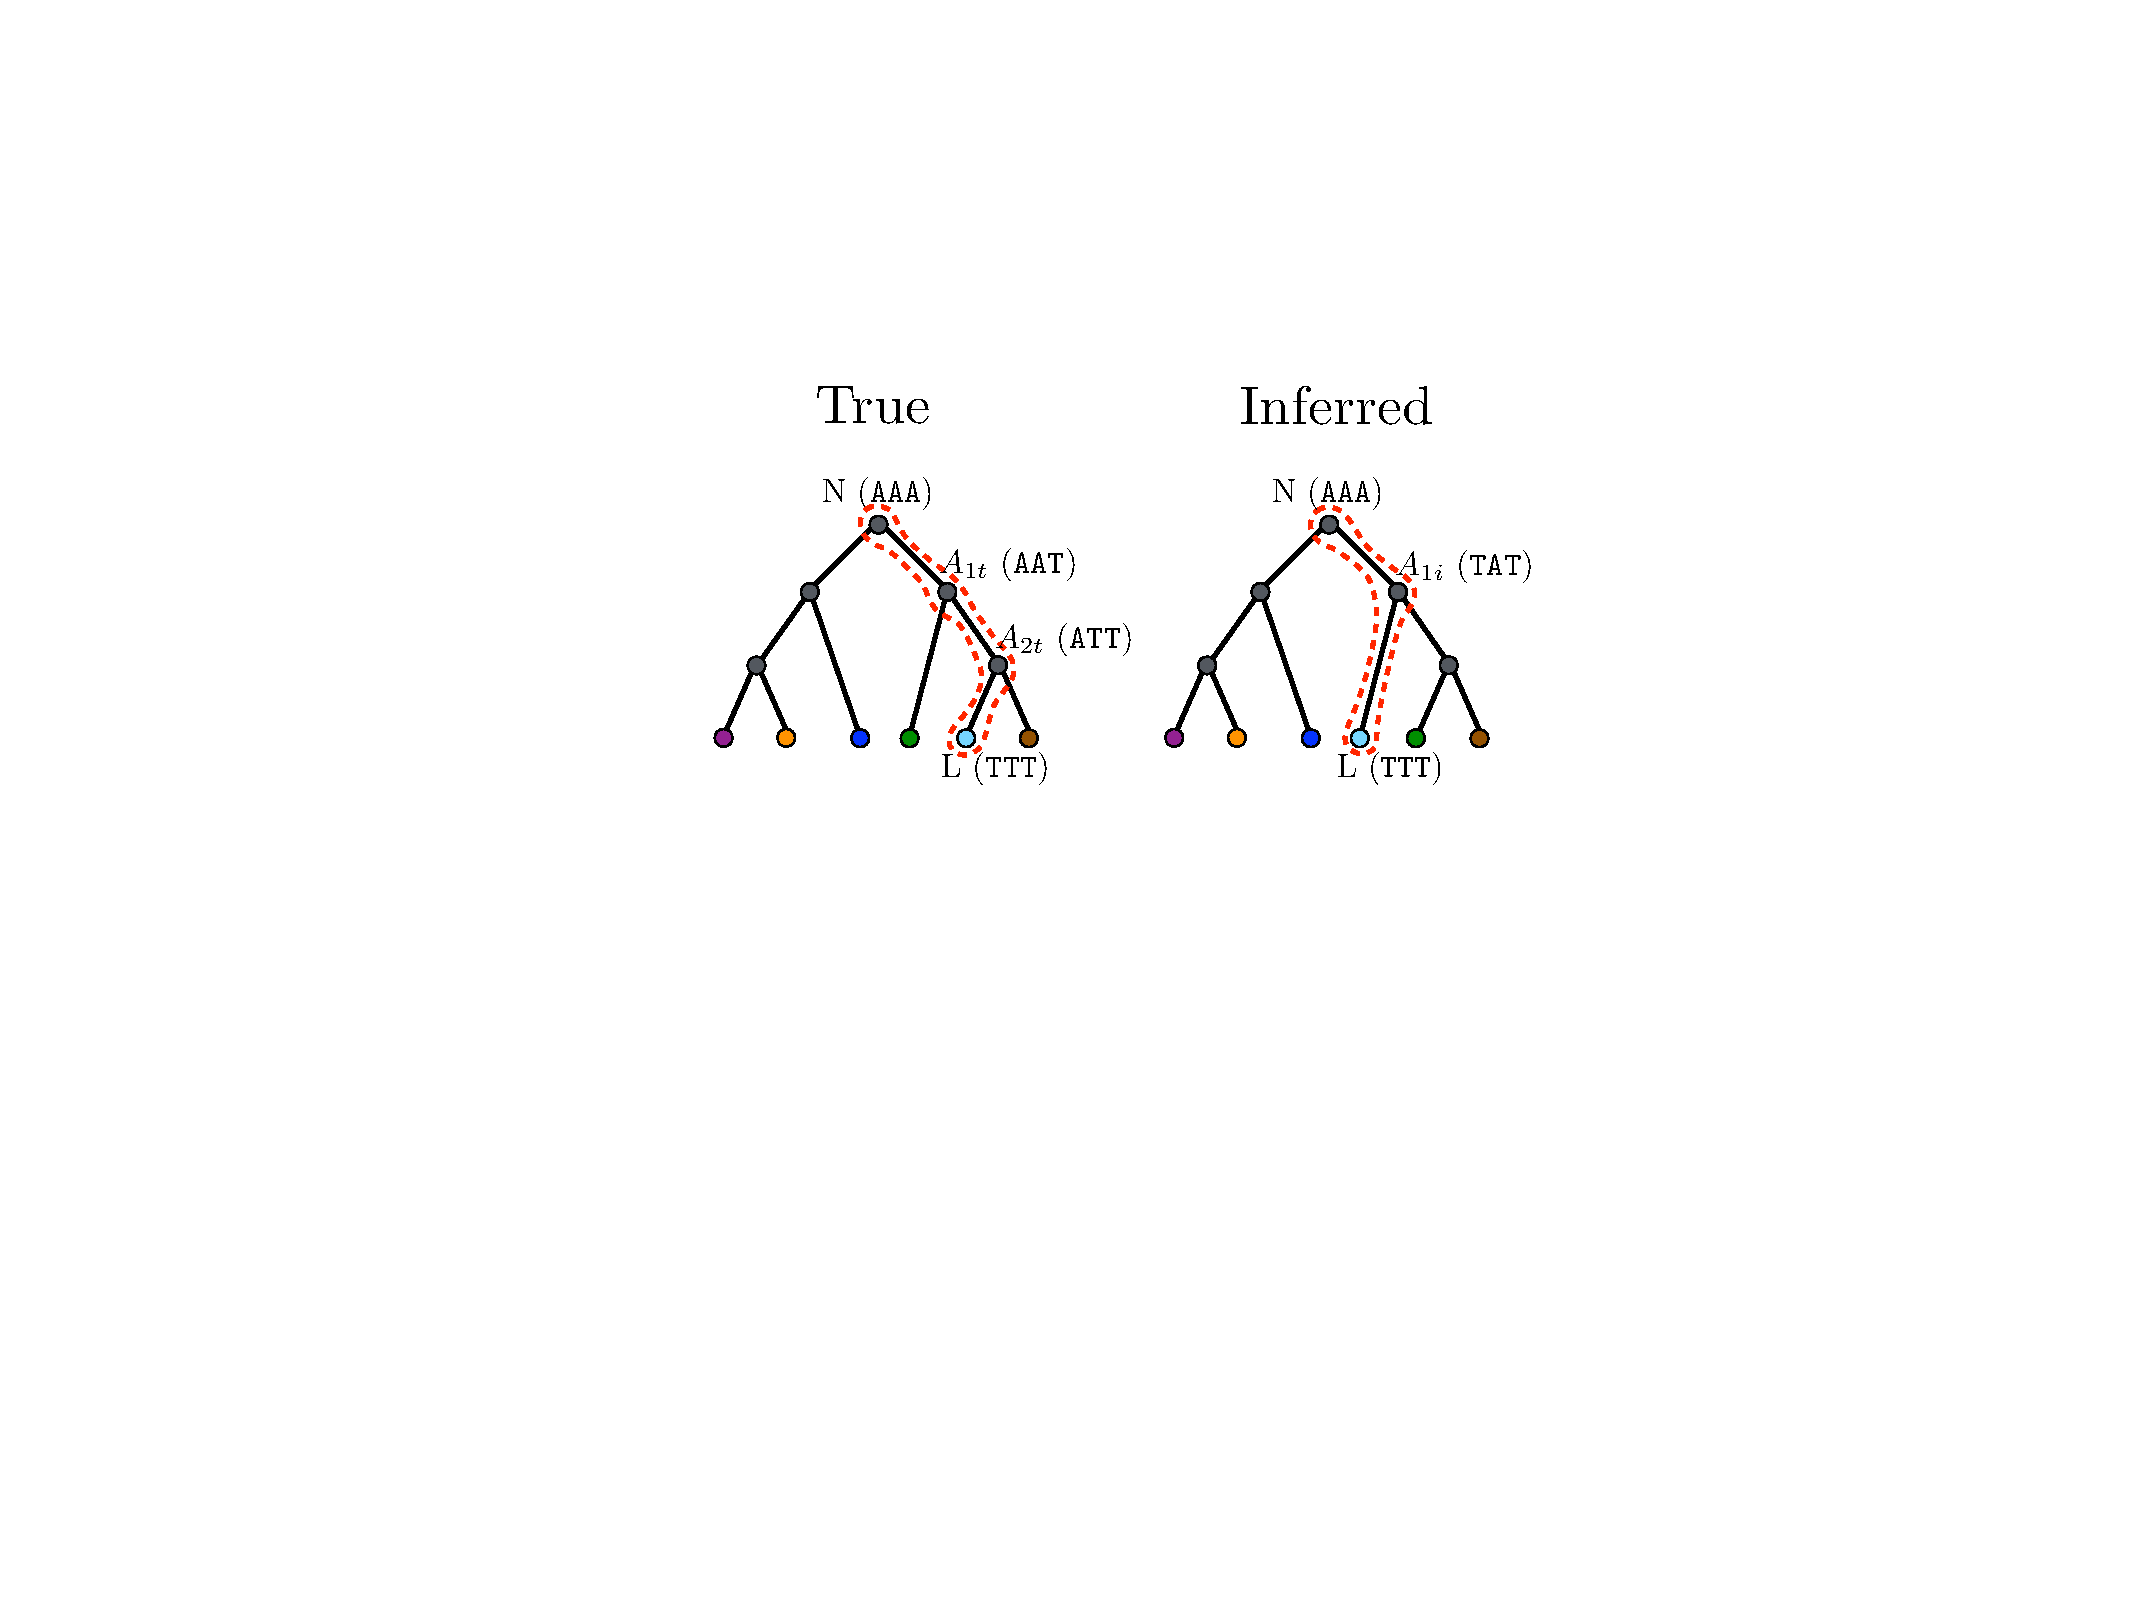
\includegraphics[width=0.7\textwidth]{figures/ASR_true_vs_inferred.pdf}
    \caption{
        \label{fig:ASR_true_vs_inferred}
        True vs.\ inferred tree with colored leaves and grey ancestral states. Reconstruction from the light blue leaf is marked by a dashed red line and annotated with genotypes in parenthesis. N is the naive sequence, L is the leaf sequence and the As are ancestors $1,2,...,n$ with either true or inferred marked by $t$ or $i$, respectively, appended to the subscript. The inferred tree has misplaced the branch leading to the light blue node, resulting in a missing ancestor sequence. The missing ancestor is treated as a missing realization in the inferred mutation process.
    }
\end{figure}



%EM I suggest reorganizing this paragraph in such a way that the definition is clear and concise. For example, we hear about gap penalties before we even know what our objective function is.
%EM You could start by describing why we are especially interested in comparing reconstructions from leaf to root, perhaps introducing the ancestral lineage, then note that these lineages can be of different lengths, making comparison non-obvious. The solution is COAR, defined as follows.
%EM fig:ASR_true_vs_inferred is a great figure for motivating COAR.
To calculate the COAR metric two lists of ancestral sequences are compared.
The lists are the ancestral sequences of all the nodes in the direct path going from a leaf to the root.
This is extracted by starting at a leaf node and traversing upwards in the tree, parent by parent, until the root is reached.
In the following, this list of sequences will be referred to as the ancestral lineage.
Two such lists are made, one for the true -and one for the inferred tree, and it is the similarity of these two lists which is the core of the COAR metric.
For lists of similar length the list comparison is easy, it will simply be the cumulated distance between the elements in the two list at the same position e.g.\ compare list 1 element 1 with list 2 element 1 and list 1 element 2 with list 2 element 2 etc.
This corresponds to the sum of hamming distances between inferred and true ancestors.
However complications arise when the lengths of the lists are not the same which can happen in the case of a wrong topology.
To make a fair comparison between the true -and inferred tree we therefore need to align the two lists and introduce a missing state, called a gap, into one of the lists.
The optimal solution to this alignment problem was described and solved by Needleman and Wunsch \cite{needleman1970general}.
We restrict the global alignment result so that it has to start at the root of the tree and end at the leaf sequence because these two states are known, or explicitly inferred, for both the true and inferred phylogenies.
We further restrict the Needleman-Wunsch algorithm so that gaps are only allowed to be introduced in the shortest of the two lists being aligned to force the maximum number of true vs.\ inferred node comparisons.
With this restriction on gaps, the number of gaps is determined solely by the differences in list lengths and as long as the gap penalty is less than or equal to zero the gaps will always be at the same positions.
Practically this means that the magnitude of the gap penalty only serves the purpose of introducing an extra penalty for inferring a wrong topology and can be adjusted to put more, or less, emphasis on tree topological correctness.
A larger gap penalty meaning more emphasis on correctness of tree topology and vice versa.

One interpretation of the COAR value is that it is the distance between the true -and inferred mutation processes as shown in figure \ref{fig:mutation_process}.
In this representation of an ancestral lineage the root and the leaf are two fixed states with a continuous mutation process running between them.
The internal nodes in the ancestral lineage is discrete states in the continues process, and while on the true tree this corresponds to a single cell, on the inferred tree no such thing exists.
Instead we can think about internal nodes on an inferred ancestral lineage as realizations along the continues mutation process defined by the inferred tree.
The COAR value is then a similarity measured between the true cell genotype and the inferred realizations, each sampled from the true -and inferred mutation processes respectively, and now in the case of a mismatch between the number of realizations and cells, a gap will be introduced in the alignment to compensate.
In this view more sequences in the inferred ancestral lineage means more realization along the mutational path and vice versa.
The important point being that that those extra realizations could in fact be correctly inferred sequences with no observations in the true phylogeny.
For this reason the gap penalty is chosen to be zero so that the COAR value will only reflect the difference in ancestral lineages and not try to address the possible differences in tree topology.
The correctness of the tree topology can the be assessed separately by other metrics e.g.\ Robinson-Foulds distance.
\begin{figure}[ht!]
    \centering
    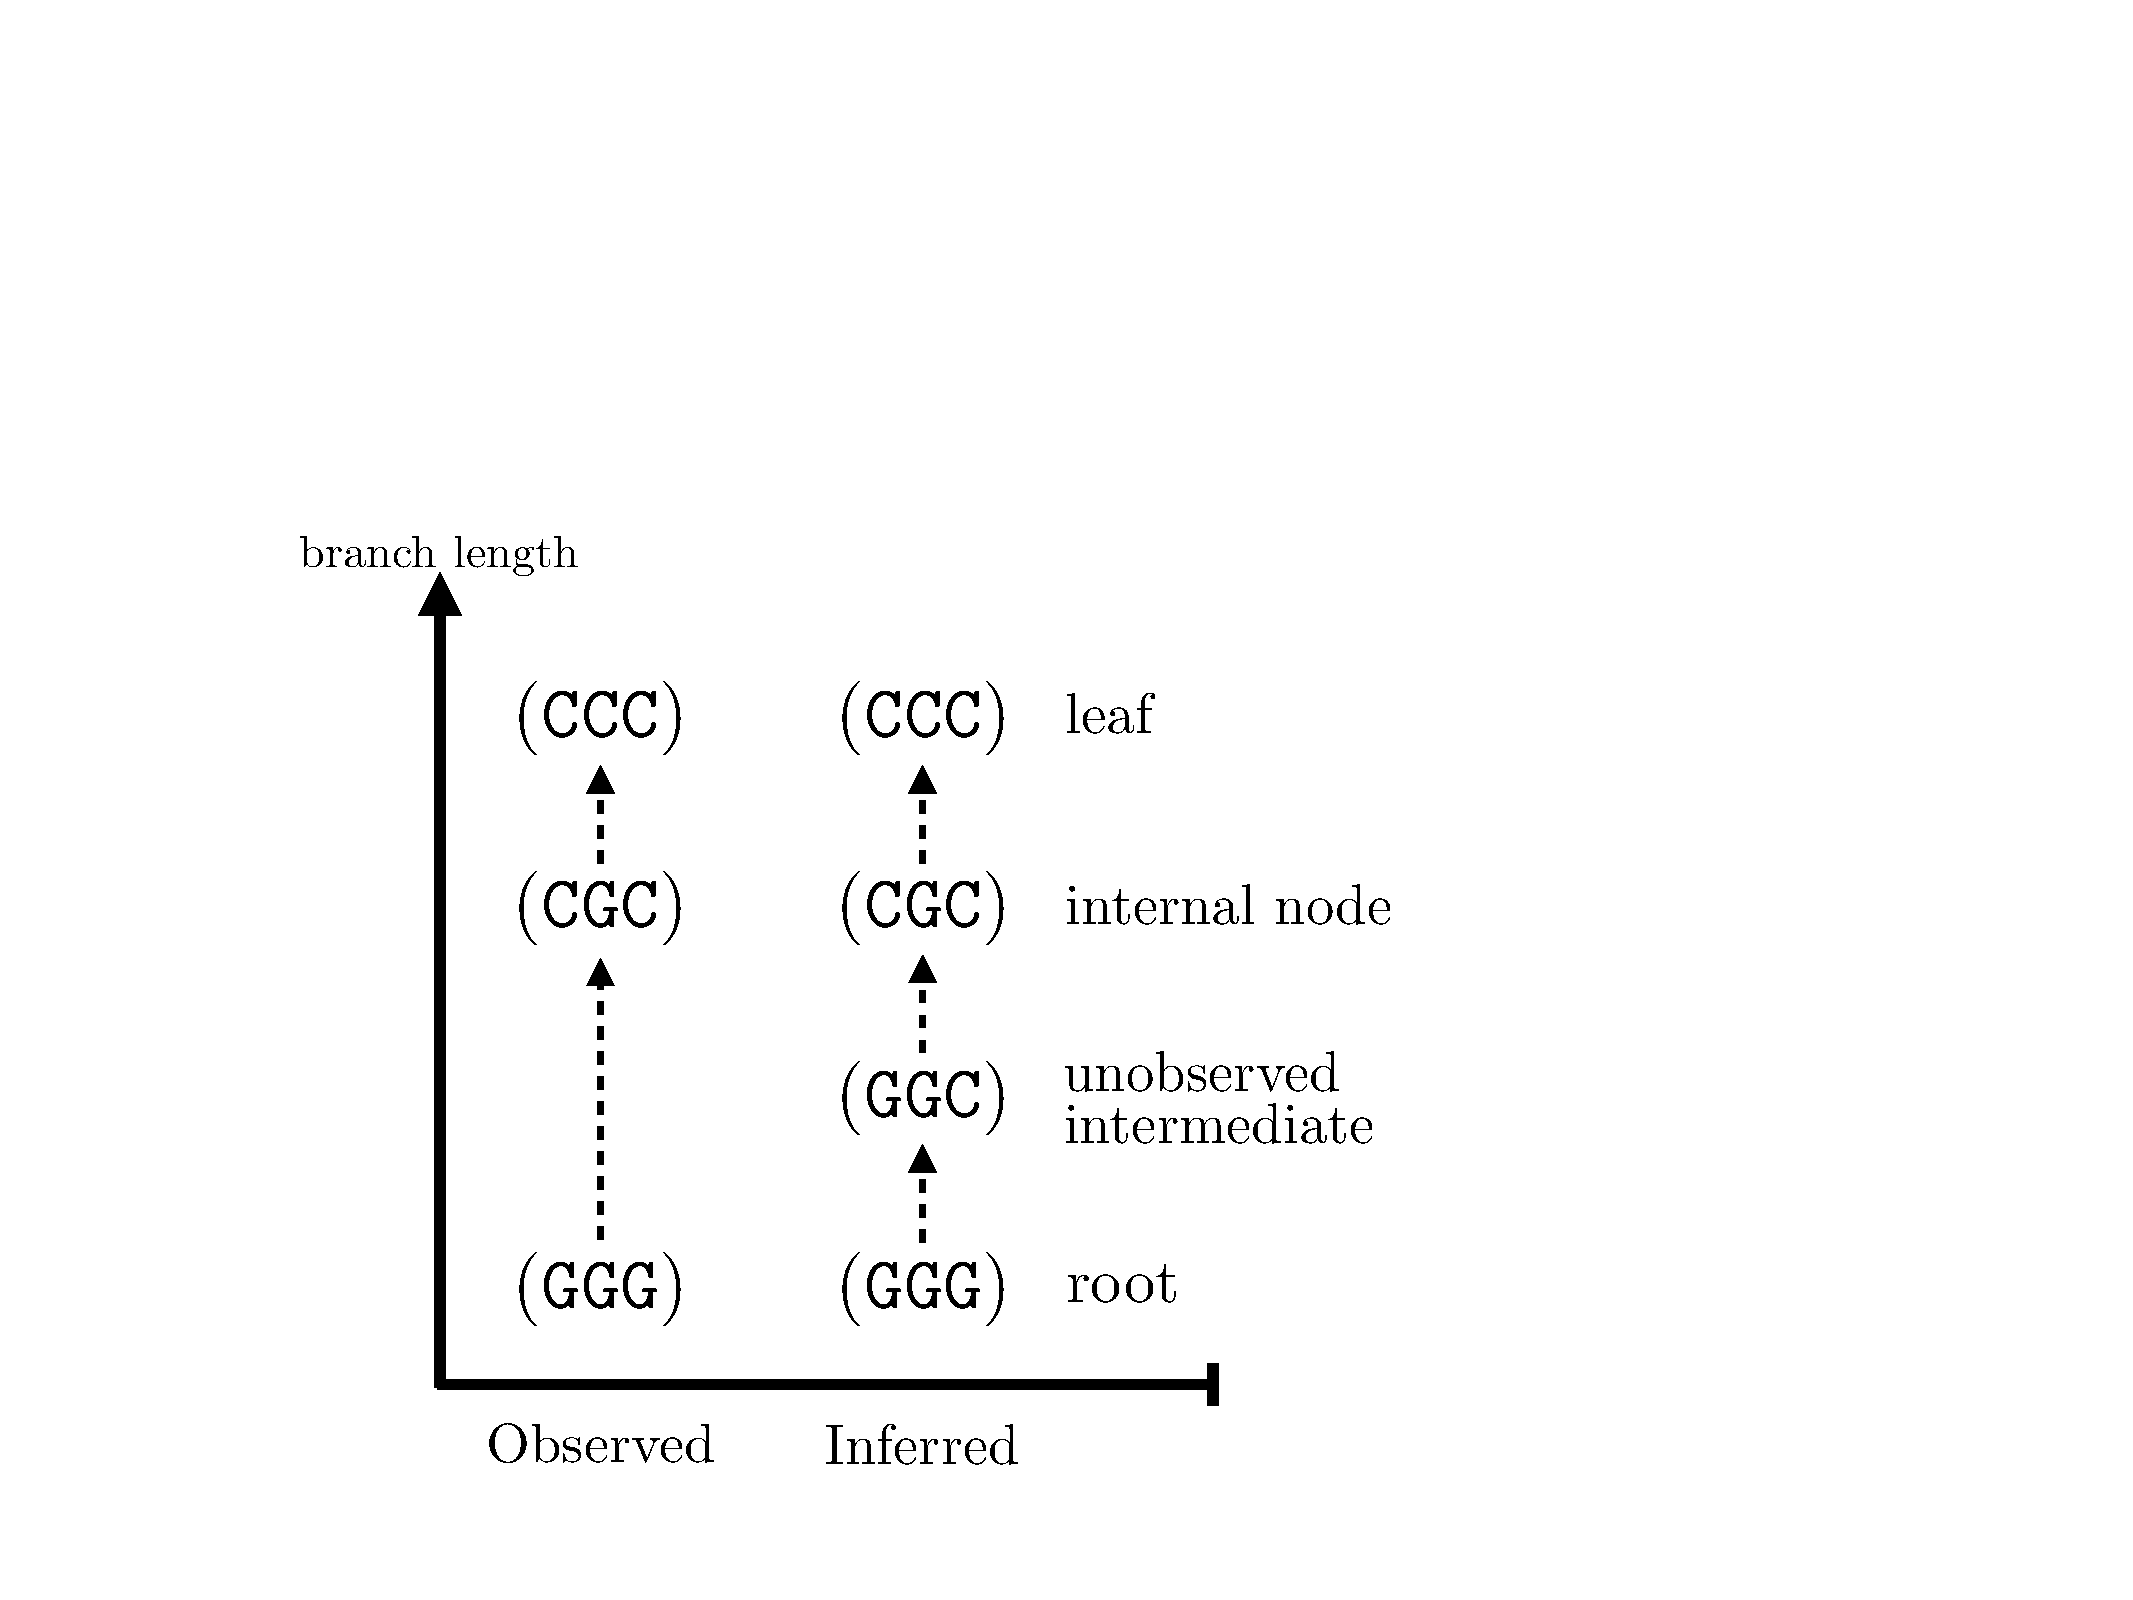
\includegraphics[width=0.5\textwidth]{figures/mutation_process2.pdf}
    \caption{
        \label{fig:mutation_process}
        One interpretation of the COAR value is that it is the distance between the true -and inferred mutation processes, here shown by the true -and inferred ancestral lineage nodes of an example phylogeny. The true ancestral lineage, left side, represents actual observed cells where the genotype is a known constant. The inferred ancestral lineage, right side, represents the estimated genotypes at branching points along the inferred topology. In some cases there is a mis-correspondence between observed cells in the true phylogeny and the branching points in the inferred tree. These are treated as missing realizations and ignored in the alignment of the two mutation processes.
    }
\end{figure}





%%% For phylogenies with known roots
%The ordered list of sequences constitute the reconstructed ancestral lineage for the leaves picked and it always start with the root sequence and ends with the leaf.
% The both the true -and inferred tree may have any number of sequences in this list however there must be as minimum 2; the root and the leaf.


Using the aligned ancestral lineages it is now possible to derive a score, similar to a sequence alignment score, and then normalizing the alignment score to the smallest possible alignment score will give our measure for correctness of ancestral reconstruction (COAR).
$$
\COAR_i = \frac{\alignscore(\leaf_i)}{\alignscore_{\min}(\leaf_i)}
$$
Where alignscore is the score of the alignment between the true and inferred ancestral lineages and in the denominator, $\alignscore_{min}$, is the smallest possible score given the number of sequences in the ancestral lineages.
The alignment score is defined in terms of penalties, so all values are negative, $\alignscore \leq 0$.
Likewise the smallest possible alignment score is negative thereby canceling out the negatives to make a positive COAR.

COAR is defined in the range from 0 to 1, where 0 is a perfect ancestral sequence reconstruction and 1 is the worst possible.
The COAR value is comparable across different trees, methods and datasets because of this normalization, and if the score is proportional to the sequence distance, COAR can be interpreted directly as the average per site error in the inferred ancestral lineage sequences.
COAR for a single ancestral lineage can be expanded to the tree level by calculating the mean COAR value for the whole tree:
$$
\operatorname{mean}(\COAR) = \sum^{L_N}_{i=1} \frac{\alignscore(\leaf_i)}{\alignscore_{\min}(\leaf_i)} / L_N
$$
Where $L_N$ is the number of leaves on the tree.




\subsubsection{Calculating COAR values - example with a known root}
As an example of how the COAR metric works we will present a small example, summarized in figure \ref{fig:ASR_true_vs_inferred} with the light blue leaf chosen for lineage reconstruction and the true and inferred ancestral lineages marked in each tree with red dashed lines.
The example is on the phylogeny of a B cell receptor (BCR) clonal family in which case the root sequence is a known state called the naive sequence.
Assume that the true phylogeny is known with corresponding ancestral sequences along the tree.
Given the leaves of this tree and their sequences a phylogeny can be inferred using any method e.g.\ maximum parsimony, maximum likelihood, Bayesian methods etc.
We make the restriction that only one inferred tree can be evaluated i.e. if multiple equally parsimonious trees exists one should be chosen at random, or using prior expectations, and if a Bayesian method is used the maximum posterior tree or a random tree weighted according to the posterior distribution should be chosen.
% The true tree will often be derived from simulations while the inferred tree can be made by many different tree algorithms nevertheless these are the basic input to determine the COAR.

%\begin{figure}[ht!]
%    \centering
%    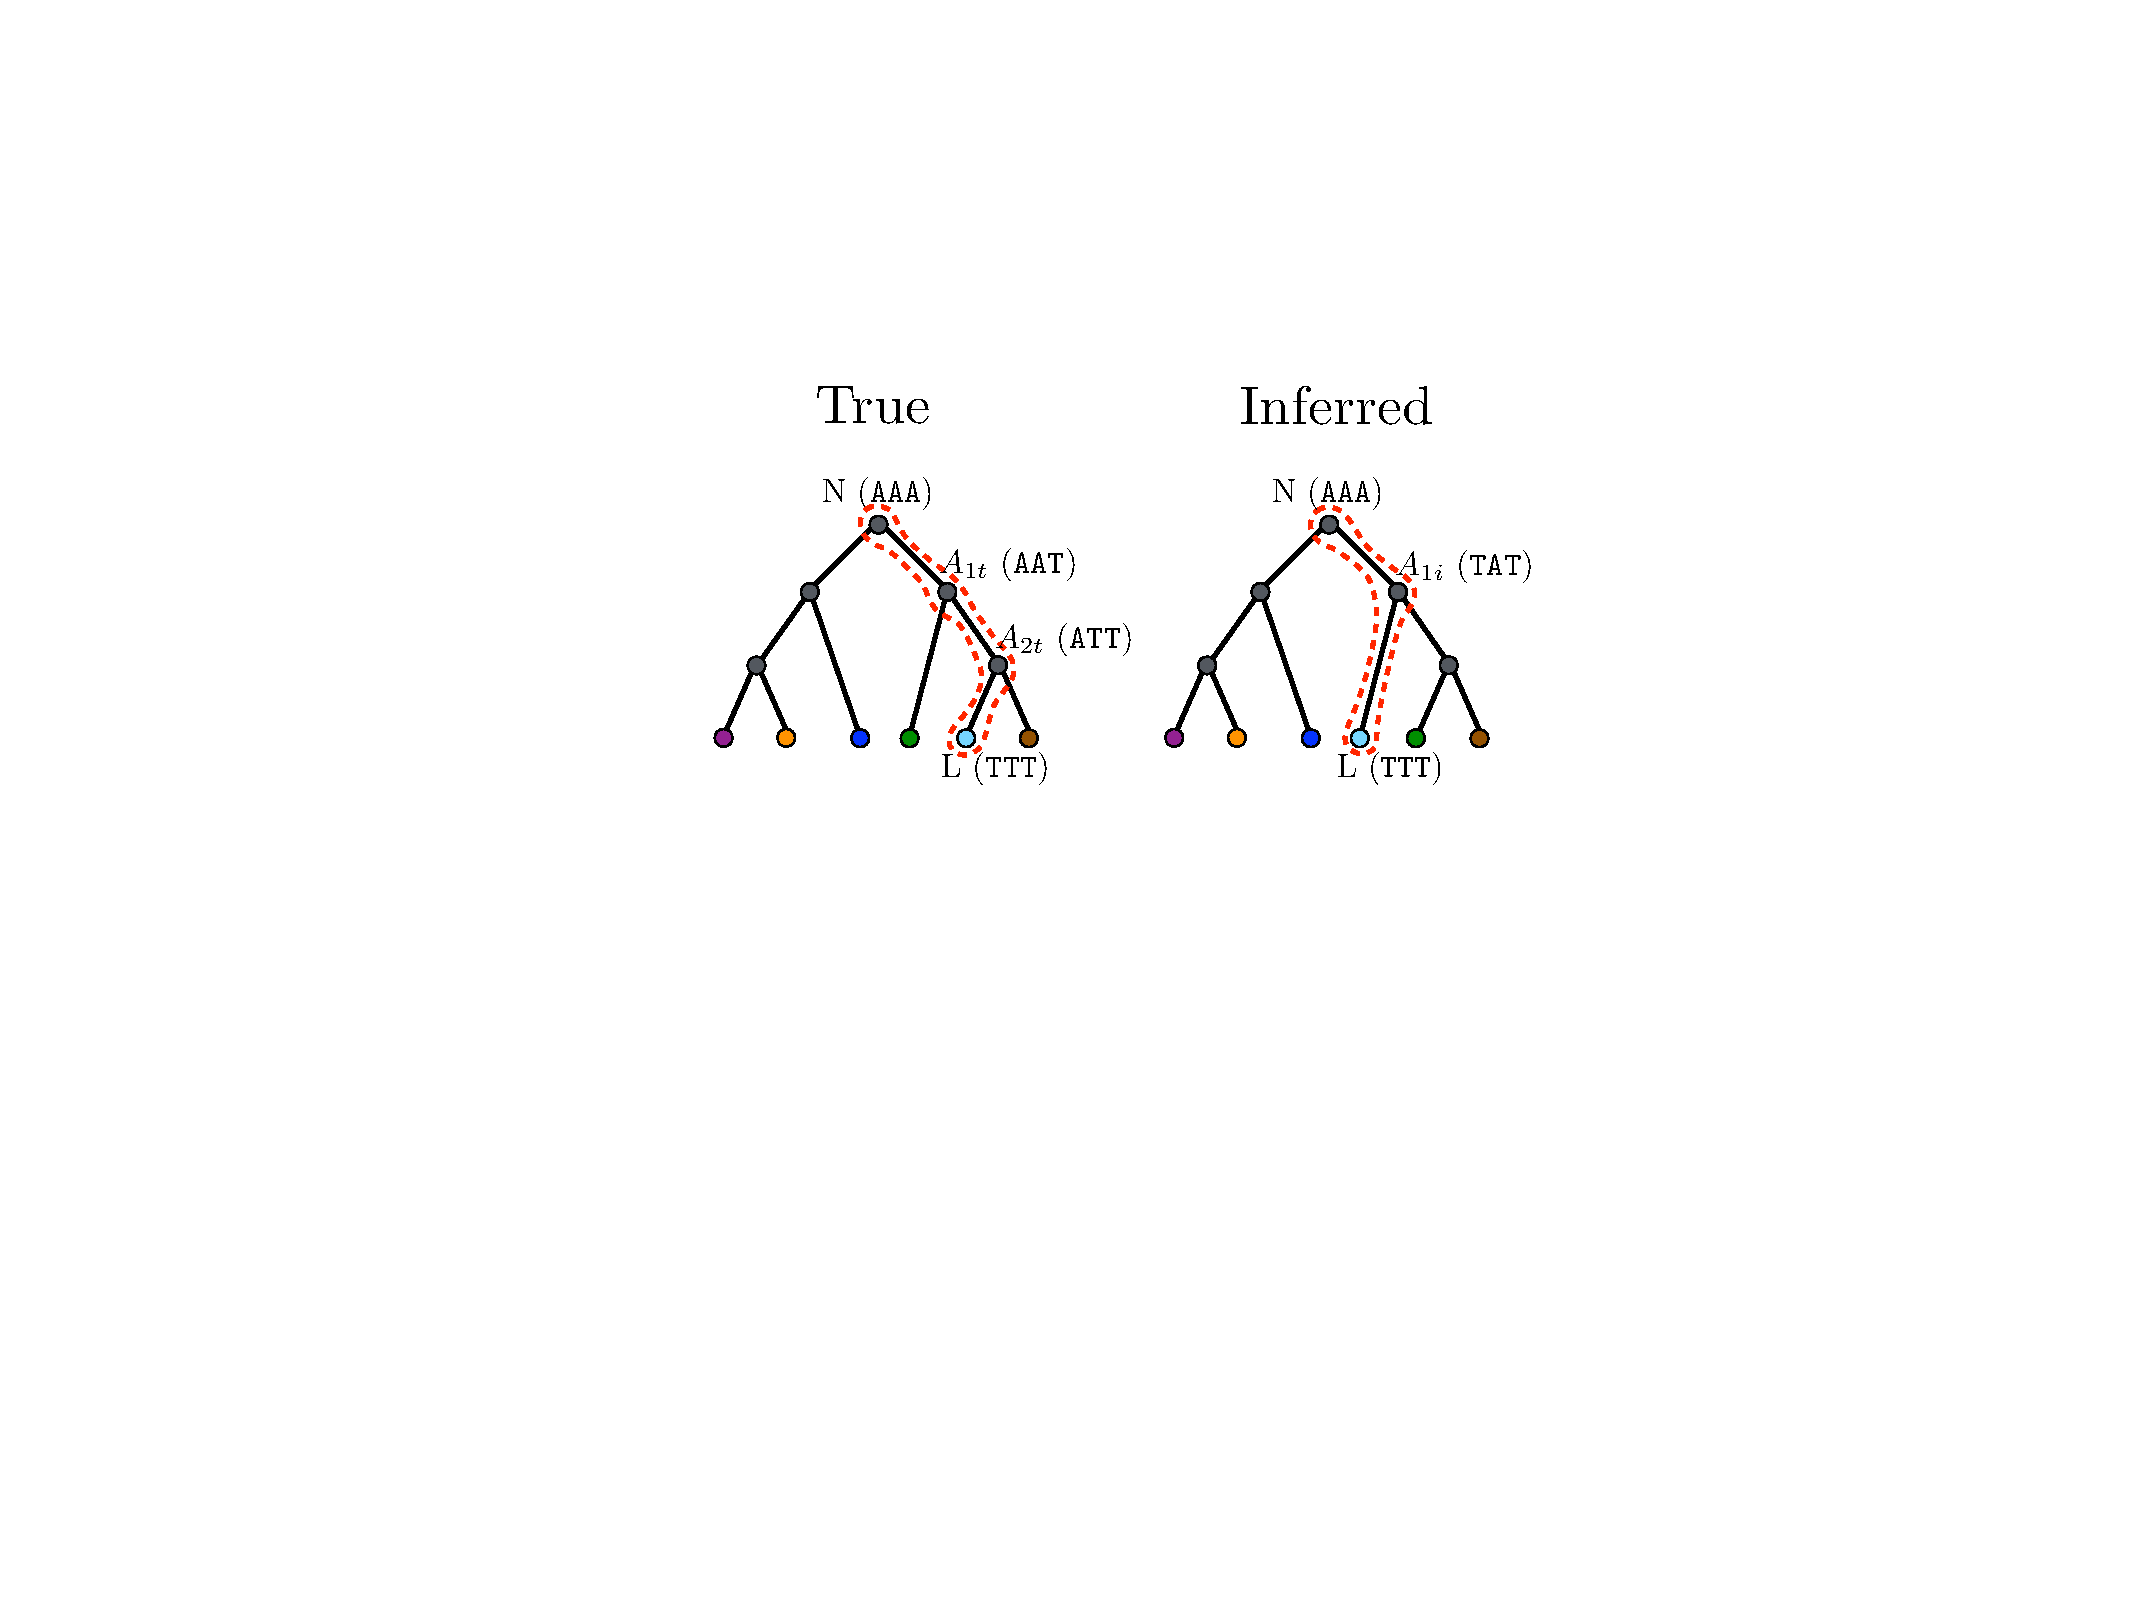
\includegraphics[width=0.7\textwidth]{figures/ASR_true_vs_inferred.pdf}
%    \caption{
%        \label{fig:ASR_true_vs_inferred}
%        True vs.\ inferred tree with colored leaves and grey ancestral states. Reconstruction from the light blue leaf is marked by a %dashed red line and annotated with genotypes in parenthesis. N is the naive sequence, L is the leaf sequence and the As are ancestors %$1,2,...,n$ with either true or inferred marked by $t$ or $i$, respectively, appended to the subscript. The inferred tree has misplaced %the branch leading to the light blue node, resulting in a missing ancestor sequence. The missing ancestor is treated as a missing %realization in the inferred mutation process.
%    }
%\end{figure}

Now take a leaf sequence on the tree and reconstruct its ancestral lineage by extracting the parent, the parent's parent, etc. until the root is reached.
Results for the trees in figure \ref{fig:ASR_true_vs_inferred} are tabulated in table \ref{true_vs_inferred_table}.
This ordered list of sequences constitute the reconstructed ancestral lineage for the chosen leaf and it always start at the root and ends with the leaf sequence.
Both the true -and inferred tree may have any number of sequences in this list, however there must be as minimum 2, the root and the leaf.
In this example the root state is known to be the naive BCR sequence, so we are imposing the restriction on the alignment that it must start with the root and end at the leaf, and that these are known states not counting towards the COAR value.

%Erick stopped here

\begin{table}[ht!]
\centering
\begin{tabular}{rcc}
\multicolumn{1}{c}{} & True   & Inferred \\ \hline
Naive (N)            & \texttt{AAA} & \texttt{AAA}         \\ \hline
$A_1$                & \texttt{AAT} & \texttt{TAT}         \\ \hline
$A_2$                & \texttt{ATT} & -                    \\ \hline
Leaf (L)             & \texttt{TTT} & \texttt{TTT}         \\ \hline
\end{tabular}
    \caption{
         \label{true_vs_inferred_table}
             Reconstructed ancestral lineage for true -and inferred trees as shown in figure \ref{fig:ASR_true_vs_inferred}.
             }
\end{table}

%%%% Maybe include abundances in the example later:
\iffalse

\begin{table}[ht!]
\centering
\label{table:true_vs_inferred_table}
\begin{tabular}{rccc}
\multicolumn{1}{c}{} & True   & Inferred & Abundance \\ \hline
Naive (N)            & \texttt{AAA} & \texttt{AAA}   & 1         \\ \hline
$A_1$                & \texttt{AAT} & \texttt{AAT}   & 2         \\ \hline
$A_2$                & \texttt{ATT} &                  & 20        \\ \hline
Leaf (L)             & \texttt{TTT} & \texttt{TTT}   & 5         \\ \hline
\end{tabular}
\end{table}

\fi

%To align the true vs.\ inferred lists of reconstructed ancestral lineages we will consider each sequence as a state that can be compared to another state to find

In cases of a wrongly inferred topology the true and inferred lists of ancestral lineage sequences can have different lengths, so we need a way of finding the best possible alignment between these lists.
We know the start and end of this alignment since that is defined as the shared root and leaf sequences, but the sequences between are free to be shifted up or down to maximize the alignment fit.
This problem is similar to that of the global sequence alignment problem solved by Needleman and Wunsch \cite{needleman1970general}.
The solution can be implemented by dynamic programming and solved in squared time complexity.
In this example phylogeny the calculation will be explicitly state by showing the matrix operations, but these operations also applies in the general case of the algorithm.
A notable difference to the original Needleman-Wunsch algorithm is that it was intended to align two sequences of characters, like DNA or amino acids, while in this application instead of aligning a list of sequence characters a list of whole sequences are aligned.

% The first step in the alignment algorithm is to calculate a distance matrix of all pairwise distances.
The first step in the alignment algorithm is to calculate a score matrix of all pairwise sequence comparisons.
For this example we use the negative of the distance between sequences as a score and therefore populating the score matrix is a simple procedure of calculating hamming distances.
However the score function can be extended to reflect different situations, like larger penalty for non-synonymous rather than synonymous mutations.
By using simple hamming distances, we will in this example be weighting all mismatches equally.
The score matrix is tabulated in table \ref{distance_matrix}.
We use negative scores to reflect that mismatches represents a loss.
% This matrix is called the score matrix to stress the fact that it is not exclusively for string distances but can accommodate more advanced loss functions.

\begin{table}[ht!]
\centering
\begin{tabular}{c|r|r|r|r}
\rowcolor[HTML]{EFEFEF}
                                 & \multicolumn{1}{c|}{\cellcolor[HTML]{EFEFEF}N} & \multicolumn{1}{c|}{\cellcolor[HTML]{EFEFEF}$A_{1t}$} & \multicolumn{1}{c|}{\cellcolor[HTML]{EFEFEF}$A_{2t}$} & \multicolumn{1}{c}{\cellcolor[HTML]{EFEFEF}L} \\ \hline
\cellcolor[HTML]{EFEFEF}N        & 0                                              & -1                                                    & -2                                                    & \multicolumn{1}{r|}{-3}                       \\ \hline
\cellcolor[HTML]{EFEFEF}$A_{1i}$ & -2                                             & -1                                                     & -2                                                    & \multicolumn{1}{r|}{-1}                       \\ \hline
\cellcolor[HTML]{EFEFEF}L        & -3                                             & -2                                                    & -1                                                    & \multicolumn{1}{r|}{0}                        \\ \hline
\end{tabular}
    \caption{
         \label{distance_matrix}
             Score matrix based on all pairwise distances between the sequence in figure \ref{fig:ASR_true_vs_inferred}.
             }
\end{table}

% To allow for different lengths of true and inferred list of ancestral sequences they are align with the possibility of a gap to be introduced.
% This gap should be penalized to reflect the difference between true and inferred ancestral lineages.
%%% Next line is true only because the gap penalty is influencing the maximum penalty and thereby shifting the COAR. It will never influence the actual alignment.
%%%%%%% This depends or whether a restriction is put on the gap introduction. E.g.\ this could be allowed:
% AA-AAA
% BBB-BB
% The magnitude of the gap penalty is determined to put appropriate amount of emphasis on correctness of the tree topology.
% In this example we will use a hard penalty on wrong topology by setting the gap penalty to -10.
% In a realistic setting the gap penalty should depend on the length of the sequences on the input tree and e.g.\ a gap penalty of 10\% of the sequence length would be sufficient to penalize wrong topologies without over emphasizing the importance compared to similarity in ancestral sequences.
% So in the example of an input tree with sequences of length 300 a gap penalty of -30 would be a good choice.
%It it worth to notice that in this example, because the first and last sequence in the alignment is fixed to the root and leaf, the number of gaps is fixed

Now we are ready to initializing the alignment grid central to the Needleman-Wunsch algorithm.
Initialization is started by inserting the scores of pure gap characters i.e. first row and first column, see table \ref{NW_fill_table1}.
Since the naive sequence is known we require the two root sequences to align by setting this gap penalty to negative infinity.
Similarly we disallow introduction of gaps in the longest of the sequence lists by penalizing these as negative infinity as seen in table \ref{NW_full_table}.
Setting certain gap penalties to negative infinity is a simple way of dealing with disallowed gaps and it works well in an implementation.
\begin{table}[ht!]
\centering
\begin{tabular}{c|r|r|r|r|r|}
\rowcolor[HTML]{EFEFEF}
                                 & \multicolumn{1}{c|}{\cellcolor[HTML]{EFEFEF}-} & \multicolumn{1}{c|}{\cellcolor[HTML]{EFEFEF}N} & \multicolumn{1}{c|}{\cellcolor[HTML]{EFEFEF}$A_{1t}$} & \multicolumn{1}{c|}{\cellcolor[HTML]{EFEFEF}$A_{2t}$} & \multicolumn{1}{c|}{\cellcolor[HTML]{EFEFEF}L} \\ \hline
\cellcolor[HTML]{EFEFEF}-        & 0                                              & -Inf                                            & -Inf                                                   & -Inf                                                   & -Inf                                            \\ \hline
\cellcolor[HTML]{EFEFEF}N        & -Inf                                            & ->                                            &                                                    &                                                    &                                             \\ \hline
\cellcolor[HTML]{EFEFEF}$A_{1i}$ & -Inf                                            &                                             &                                                    &                                                    &                                             \\ \hline
\cellcolor[HTML]{EFEFEF}L        & -Inf                                            &                                             &                                                    &                                                    &                                             \\ \hline
\end{tabular}
    \caption{
         \label{NW_fill_table1}
             The starting alignment grid, initialized with the gap penalties which is negative infinity to disallow gap opening in the beginning of the alignment. The grid is filled up from left to right row by row, starting in the cells with left, top and diagonal cells filled (marked by ->).
             }
\end{table}


Then the alignment grid is filled up starting with the cell that has left, top and diagonal cells filled (marked by -> in table \ref{NW_fill_table1}) and continuing to the right side cell that also has left, top and diagonal cells filled.
Each cell is filled up by the following equation:
$$
C_{i,j} = max\left\{ (C_{i-1,j} + gp_{down}); (C_{i,j-1} + gp_{right}); (C_{i-1,j-1} + SC_{i-1,j-1})  \right\}
$$
Moving in the order $i=1,2,3,4$ and $j=1,2,3,4,5$. Where $C_{i,j}$ is the ith row and jth column cell in the grid, $SC_{i-1,j-1}$ is the score of aligning the ith, jth elements found by look-up in the the score matrix (table \ref{distance_matrix}) and $gp_{down}$ and $gp_{right}$ is the gap penalty of the moving down and right respectively.
In this example the longest sequence list is the true ancestral lineage and therefore gaps are only allowed to be introduced into the inferred list of sequences.
The penalty for introducing gaps in the true list of sequences is set to negative infinity to reflect this and therefore $gp_{down} = -\Inf$ and $gp_{right} = 0$.

The grid is filled and results store in table \ref{NW_full_table}.
The final alignment score is the number in the rightmost bottom cell.
\begin{table}[ht!]
\centering
\begin{tabular}{c|r|r|r|r|r|}
\rowcolor[HTML]{EFEFEF}
                                 & \multicolumn{1}{c|}{\cellcolor[HTML]{EFEFEF}-} & \multicolumn{1}{c|}{\cellcolor[HTML]{EFEFEF}N} & \multicolumn{1}{c|}{\cellcolor[HTML]{EFEFEF}$A_{1t}$} & \multicolumn{1}{c|}{\cellcolor[HTML]{EFEFEF}$A_{2t}$} & \multicolumn{1}{c|}{\cellcolor[HTML]{EFEFEF}L} \\ \hline
\cellcolor[HTML]{EFEFEF}-        & 0                                              & -Inf                                            & -Inf                                                   & -Inf                                                   & -Inf                                            \\ \hline
\cellcolor[HTML]{EFEFEF}N        & -Inf                                            & 0                                              & 0                                                   & 0                                                   & 0                                            \\ \hline
\cellcolor[HTML]{EFEFEF}$A_{1i}$ & -Inf                                            & -Inf                                            & -1                                                     & -1                                                   & -1                                            \\ \hline
\cellcolor[HTML]{EFEFEF}L        & -Inf                                            & -Inf                                            & -Inf                                                   & -2                                                    & -1                                            \\ \hline
\end{tabular}
    \caption{
         \label{NW_full_table}
             The filled alignment grid, ready for tracing back the best alignment. The rightmost bottom cell has the score for the best alignment.
             }
\end{table}

Last step is to traceback the best path through the alignment grid and store this alignment.
The traceback starts from the leaf sequence, in the right bottom corner, and ends with the naive sequence in the left top corner.
A diagonal step is equivalent to a sequence match, a left move is introducing a gap character in the inferred list and a move up is introducing a gap in the true list.
The path is found by moving backwards following the same path that was used to fill up the grid, and therefore using the same equation as to fill it, just reversed with moving from bottom right cell to top left, $i=4,3,2,1$ and $j=5,4,3,2,1$:
%$$
%move_{i,j} = which\left\{ (C_{i-1,j} + gp_{down} = C_{i,j}); (C_{i,j-1} + %gp_{right} = C_{i,j}); (C_{i-1,j-1 } + SC_{i-1,j-1} = C_{i,j})  \right\}
%$$
$$
move_{i,j} = which\left\{ C_{i,j} = [(C_{i-1,j} + gp_{down}), (C_{i,j-1} + gp_{right}), (C_{i-1,j-1 } + SC_{i-1,j-1})] \right\}
$$
Notice that this path has already been generated when the alignment grid was filled up and could be cached. The resulting alignment and the penalty for each position is tabulated in table \ref{NW_final_alignment}.

Lastly this value is normalized by the smallest possibly alignment score assuming that all matched positions contained sequences with maximal distances i.e. no similarity, this normalized number is the COAR values and it runs between 0 to 1.
In the presented example we only calculated the COAR value for the reconstructed ancestral lineage from one leaf node but doing the calculations on all leaves on the tree and taking the average would give the the mean COAR value for the whole tree.
% Doing the same calculations on all leaves on the tree and summing this will give the total alignment score of the inferred phylogeny.
\begin{table}[ht!]
\centering
\begin{tabular}{|lcccc|}
\hline
\multicolumn{1}{|l|}{True}     & \multicolumn{1}{c|}{N} & \multicolumn{1}{c|}{$A_{1t}$} & \multicolumn{1}{c|}{$A_{2t}$} & T                      \\
\multicolumn{1}{|l|}{Inferred} & \multicolumn{1}{c|}{N} & \multicolumn{1}{c|}{$A_{1i}$} & \multicolumn{1}{c|}{-}        & T                      \\ \hline
Penalty                        & 0                      & -1                             & 0                           & 0                      \\ \hline
Max penalty                    & \multicolumn{1}{l}{0}  & \multicolumn{1}{l}{-3}        & \multicolumn{1}{l}{0}       & \multicolumn{1}{l|}{0} \\ \hline
COAR                           & \multicolumn{4}{c|}{-1/-3=0.333}                                                                                    \\ \hline
\end{tabular}
    \caption{
         \label{NW_final_alignment}
             The resulting alignment and the penalty for each positions.
             }
\end{table}





\subsection{Other validation metrics}

\subsubsection{Most recent common ancestor distance}
As an alternative to COAR we are also using a measure named the "most recent common ancestor" (MRCA) metric.
In this more simple measure of correctness of ASR the MRCA ancestral sequence between two leaves are found and compared in the true vs.\ inferred phylogeny.
By iterating through all pairwise combinations of leaves the MRCA distance can be found as the sum:
$$
\MRCA_{\dist} = \sum_{i=1}^{N} \sum_{j=i+1}^{N} \dist(T_{MRCA}(l_i, l_j), I_{MRCA}(l_i, l_j))
$$
All the pairwise combinations of leaves $l_i$ and $l_j$ ($i \neq j$) to find their true ($T_{MRCA}$) -and inferred ($I_{MRCA}$) MRCA.
The distance between the two ancestral sequences are found with the function $\dist(\cdot, \cdot)$ and summed over all pairs.
In this work we use the hamming distance as distance function.

Similar to COAR, ancestral sequences close to the root will have more influence on the result than sequences close to the tips.
The major difference is that MRCA is not scaled and not representing the result of a lineage reconstruction and can therefore the value has no meaningful interpretation aside from measuring performance of different method on identical data.


\subsubsection{Robinson–Foulds distance}
The tree topology is the model that explains the order of branching events and relatedness of leaves, and therefore inferred ancestral sequences will always be tied to the topology.
Hence validating the ASR should also express some degree of correctness of the tree.
Regardless it is interesting to have a method solely expressing the correctness of inferred tree topology so for this purpose we use the Robinson–Foulds (RF) distance \cite{robinson1981comparison}.
Briefly the RF distance is defined as the number of different tree partitions between two trees.
Tree partitions are made by cutting a branch connecting two nodes, all possible cuts are performed and the resulting split of taxa are sorted and recorded into two columns.
The after sorting the list of partitions they are compared true vs.\ inferred tree and for each partition mismatch the RF distance is increased by 1.



\subsection{Algorithms tested}
With the exception of a few methods there has been little published about BCR phylogeny specific software.
Barak et al. made some vaguely defined rules written into a an algorithm they named IgTree \cite{Barak2008-fw}.
The description of IgTree is similar to that of maximum parsimony (MP) and it is unclear whether there is any difference at all.
For that reason we use the MP algorithm \texttt{dnapars} from PHYLIP \cite{plotree1989phylip} as a substitute for IgTree and other methods e.g.\ Tas et al. \cite{tas2016visualizing}.

In the paper from Doria-Rose et al. \cite{Doria-Rose2014-vi} they use the general time reversible (GTR) model implemented in MEGA5 \cite{tamura2011mega5}.
Similarly Kepler \cite{Kepler2013-sy} was using \texttt{dnaml} from the PHYLIP package to infer BCR phylogenetic trees.
To test these commonly used maximum likelihood trees we use \texttt{dnaml}.

Two different models have been defined specifically for BCR evolution on protein level, the AB amino acid substitution matrix from Mirsky et al. \cite{mirsky2014antibody} and HLP17 codon model from Hoehn et al. \cite{Hoehn2016-wg}.
Both are implemented with codonPhyML \cite{gil2013codonphyml}.
The AB substitution matrix is just a standard amino acids substitution rate matrix but fitted to substitutions observed in BCR sequences, yielding a symmetric rate matrix that assumes equilibrium.
But recently Sheng et al. found large discrepancies between their findings and the AB substitution matrix \cite{sheng2017gene}, promoting us to exclude this from our evaluation.
Instead we test the HLP17 model as it is implemented in the software IgPhyML (\url{github.com/kbhoehn/IgPhyML}).
The HLP17 model is based on a GY94 model \cite{goldman1994codon} but adding parameters to account for AID hot/cold spots and thereby attempting to address the context sensitivity of SHM.

Lastly we also test the performance of an unpublished method that uses a likelihood based ranking of equally parsimonious trees, we call this method GCtree, for genotype collapsed tree.
Briefly, the likelihood function is based on the assumption that the GC reaction can be modelled as a binary Galton-Watson process \cite{harris2002theory}.
Some genotypes have many observations while others have fewer, the Galton-Watson process will favour a high abundance genotype to be the parent for a low abundance genotype.
Each MP tree is evaluated and ranked according to its fit and then the highest likelihood tree is picked out as the GCtree inferred tree.



\subsection{Simulated data}
Simulations were performed using both the neutral branching process and the affinity simulation previously described in chapter 3.
Both simulation, inference and evaluation was wrapped into an SCons script \cite{fomel2007reproducible} available in the codebase of \texttt{GCtree} (\url{github.com/matsengrp/gctree}).
SCons commands used can be found in appendix C.





\section{Results - comparing algorithms for B cell phylogenetic reconstruction}
The most suitable dataset for clonal family phylogeny is dara collected from a single GC like one in Tas et al. \cite{tas2016visualizing}.
But unlike single cell sequences most data is generated from bulk RNA extract from peripheral blood mononuclear cell (PBMC).
To adjust the simulation parameters to recapitulate a given dataset we both used the single cell Tas dataset (see appendix B), and an HTS dataset generated from PBMCs from HIV infected individuals.
In these HTS datasets cluster were done using partis resulting in hundreds of clonal families.
To only isolate HIV relevant clonal families a seed sequence was used and only sequence in the same clonal family was extracted.
Seed sequences were generated by single cell screening of the memory fraction of the PBMCs, followed by Sanger sequencing of the cells expressing HIV neutralizing antibodies.
The size of the clonal families varied substantially as shown in figure \ref{fig:Laura-neutsim_Laura-data}, but they serve as a more realistic dataset case than the single cell data from Tas et al.


Simulation parameters are adjusted in order to recapitulate two measures: a) distribution of sequence across the length of the tree and b) how "spread out" the tree leaves.
Measure a) is captured by plotting the CDF of the distance to the naive/root sequence ((a) in figure \ref{fig:Laura-neutsim_Laura-data} and \ref{fig:Laura-affsim_Laura-data}).
Measure b) is captured by plotting the CDF of the nearest neighbor distance ((b) in figure \ref{fig:Laura-neutsim_Laura-data} and \ref{fig:Laura-affsim_Laura-data}).
The neutral simulation with a high $\lambda$ will naturally vary a lot early population size an therefore had no problem fitting into the large span of possible summary statistics defined by two chosen clonal family representatives from the HTS data, see figure \ref{fig:Laura-neutsim_Laura-data}.
The nature of the affinity simulation forces it to have a rather constant population size defined by its carrying capacity.
Instead the GC was down-sampled to 150 sequence and the variance in the number of observed sequences comes from the fact that some sequences are identical at DNA level and deduplicated, see figure \ref{fig:Laura-affsim_Laura-data}.

\begin{figure}[!ht]
    \begin{center}
    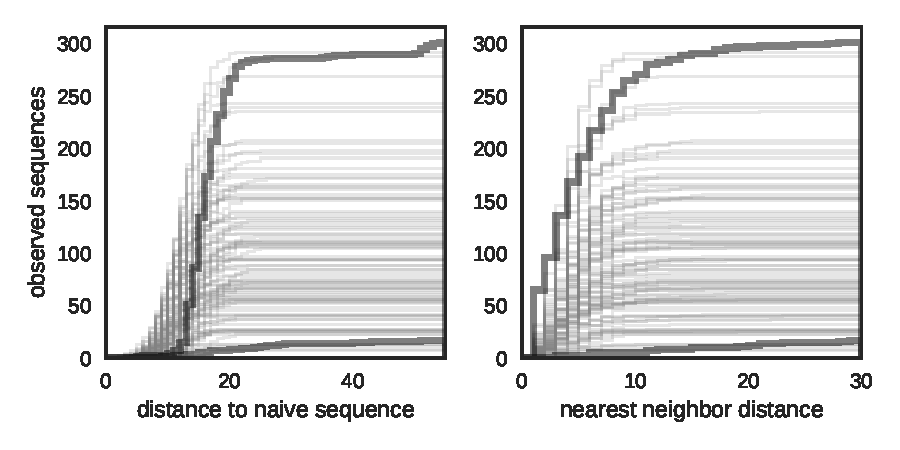
\includegraphics[width=0.8\textwidth]{figures/Laura-neutsim_Laura-data.pdf}\newline%
    \end{center}
    \vspace{-14mm} \hspace{44mm} (a) \hspace{50mm} (b)
    \caption{
        \label{fig:Laura-neutsim_Laura-data}
        Summary statistics for the unique sequences simulated under a neutral model fitted to HTS data.
        The two thick dark grey lines represents the characteristics of two clonal families extracted by partis seed clustering on HTS data.
        Smaller light grey lines are showing 1 of the 100 simulated datasets.
        Non default parameters used: $T=5$, $\lambda=2.5$, $\lambda_0=3$
    }
\end{figure}

\begin{figure}[!ht]
    \begin{center}
    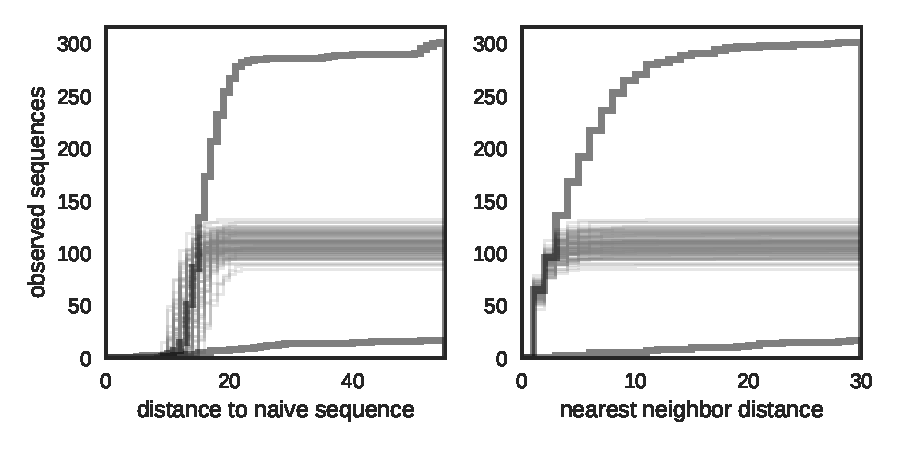
\includegraphics[width=0.8\textwidth]{figures/Laura-affsim_Laura-data.pdf}\newline%
    \end{center}
    \vspace{-14mm} \hspace{44mm} (a) \hspace{50mm} (b)
    \caption{
        \label{fig:Laura-affsim_Laura-data}
        Summary statistics for the unique sequences simulated under the affinity model fitted to HTS data.
        The two thick dark grey lines represents the characteristics of two clonal families extracted by partis seed clustering on HTS data.
        Smaller light grey lines are showing 1 of the 100 simulated datasets.
        Non default parameters used: $T=90$, $n=150$, $\lambda_0=0.25$
    }
\end{figure}


Looking a RF distance for the neutral simulation there are only small differences and only the distribution of RF distances for MP is shift up compared to the others (significant $p<0.05$ in Mann–Whitney U (MWU) test), see figure \ref{fig:Laura-neutsim_valid}.
Likewise the quartiles are slightly shifted upward for MP in the comparison of MRCA distances.
We consider COAR the most important metric because this has a direct interpretation inspired by the purpose of the tree, and for COAR there seems to be no significant difference between the methods when simulating under neutral conditions.
The average COAR values are ranging from 1.76E-04 to 2.37E-04 (appendix A table \ref{tab:Laura-neutsim_vali}) corresponding to approx. 10\% chance of one nucleotide error per reconstructed sequence in a lineage from leaf to root.
Similar but somewhat large differences are observed for neutral simulation using parameters fitted to the Tas dataset, see figure \ref{fig:Tas-neutsim_vali} in appendix B.
Should we rank the methods based on all metrics from best to worst the rank would be: GCtree, dnaml, IgPhyML, Parsimony.
But the first three are virtually the same.
The Tas dataset fitted simulations also experience a similar range of expected errors in ASR, though slightly lower because of the fewer sequences simulated, see table \ref{tab:Tas-neutsim_vali} in appendix A.

\begin{figure}[!ht]
    \centering
    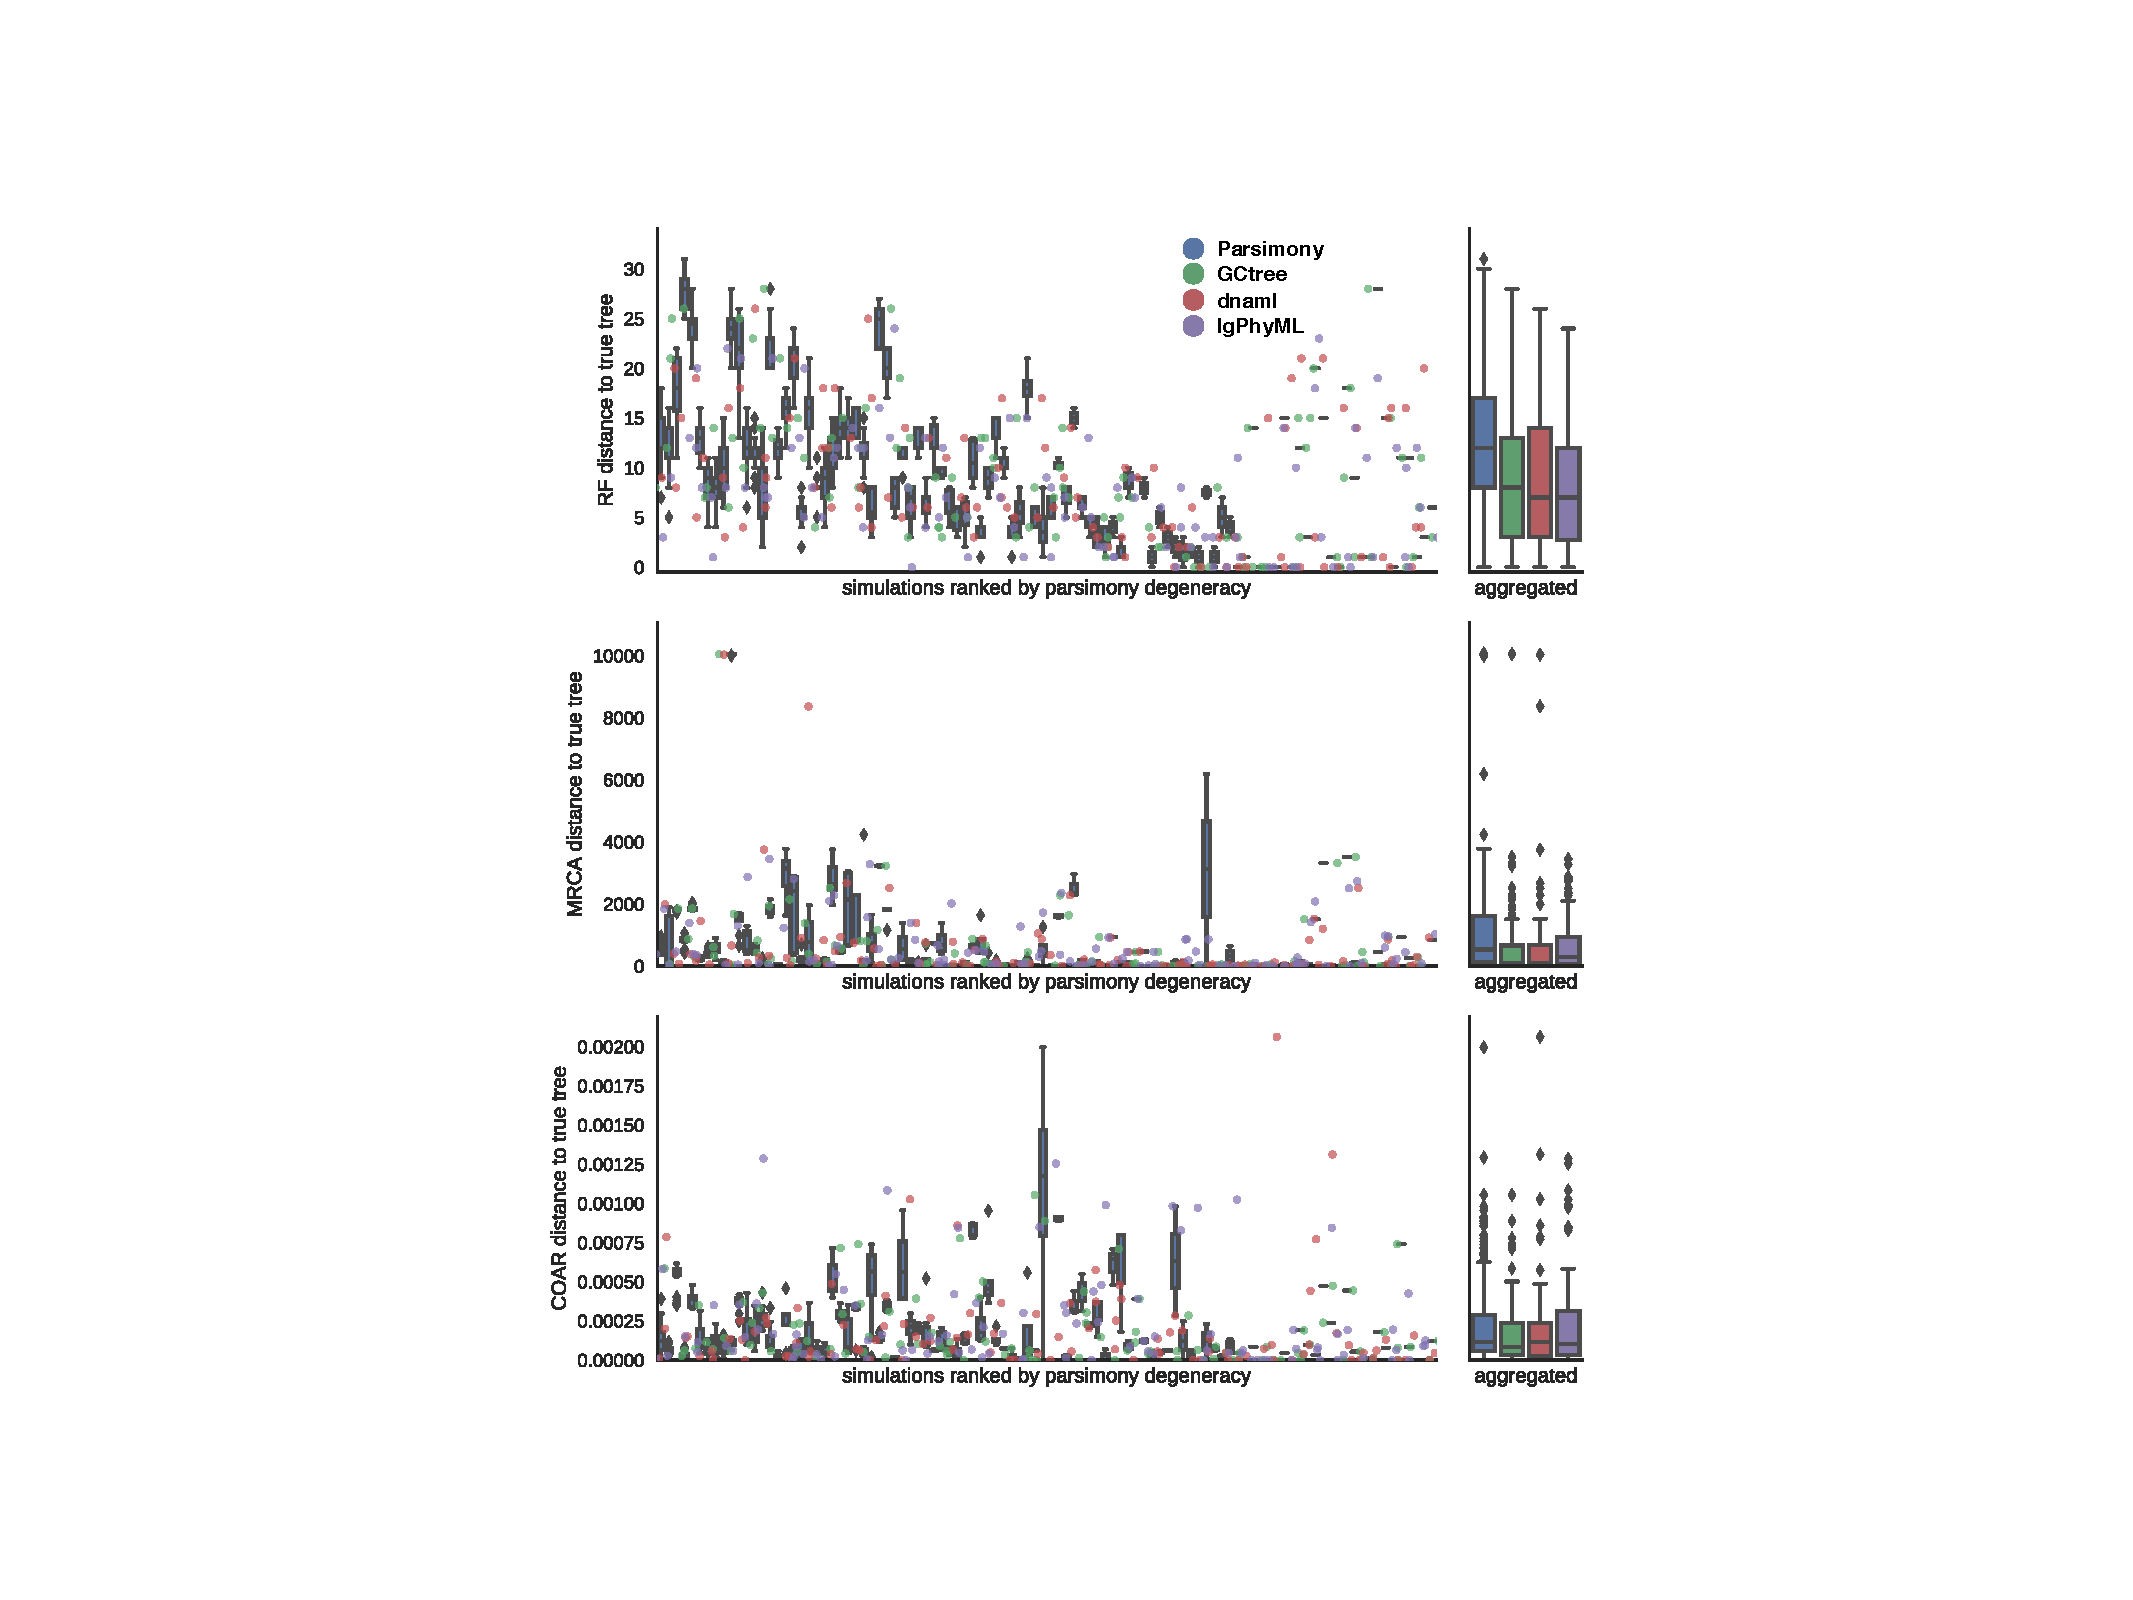
\includegraphics[width=0.9\textwidth]{figures/Laura-neutsim_valid.pdf}
    \caption{
        \label{fig:Laura-neutsim_valid}
        Simulation with 100 repeats of a neutral branching process.
        Each simulation is plotted in a single column ranked according to the number of equally parsimonious trees for the simulation.
        The ensemble of equally parsimonious trees are shown as a box plot while the other methods are plotted as jittered dots.
        On the right the aggregated result is shown.
    }
\end{figure}
\clearpage


For the affinity simulations we allow genotypes to reappear in another clade during simulations i.e. homoplasy is allowed.
This prevents us from calculating the RF distance but not from the other metrics.
However for both MRCA and COAR there is no significant differences resulting in a tie between all the inference methods, see figure \ref{fig:Laura-affsim_valid}.
Similar characteristics are observed for affinity simulations fitted to the Tas dataset, although with slightly worse performance of MP and IgPhyML, see figure \ref{fig:Tas-affsim_vali} in appendix B.
Again the best to worse rank would be: GCtree, dnaml, IgPhyML, Parsimony, but with a small effect size separating them.

\begin{figure}[!ht]
    \centering
    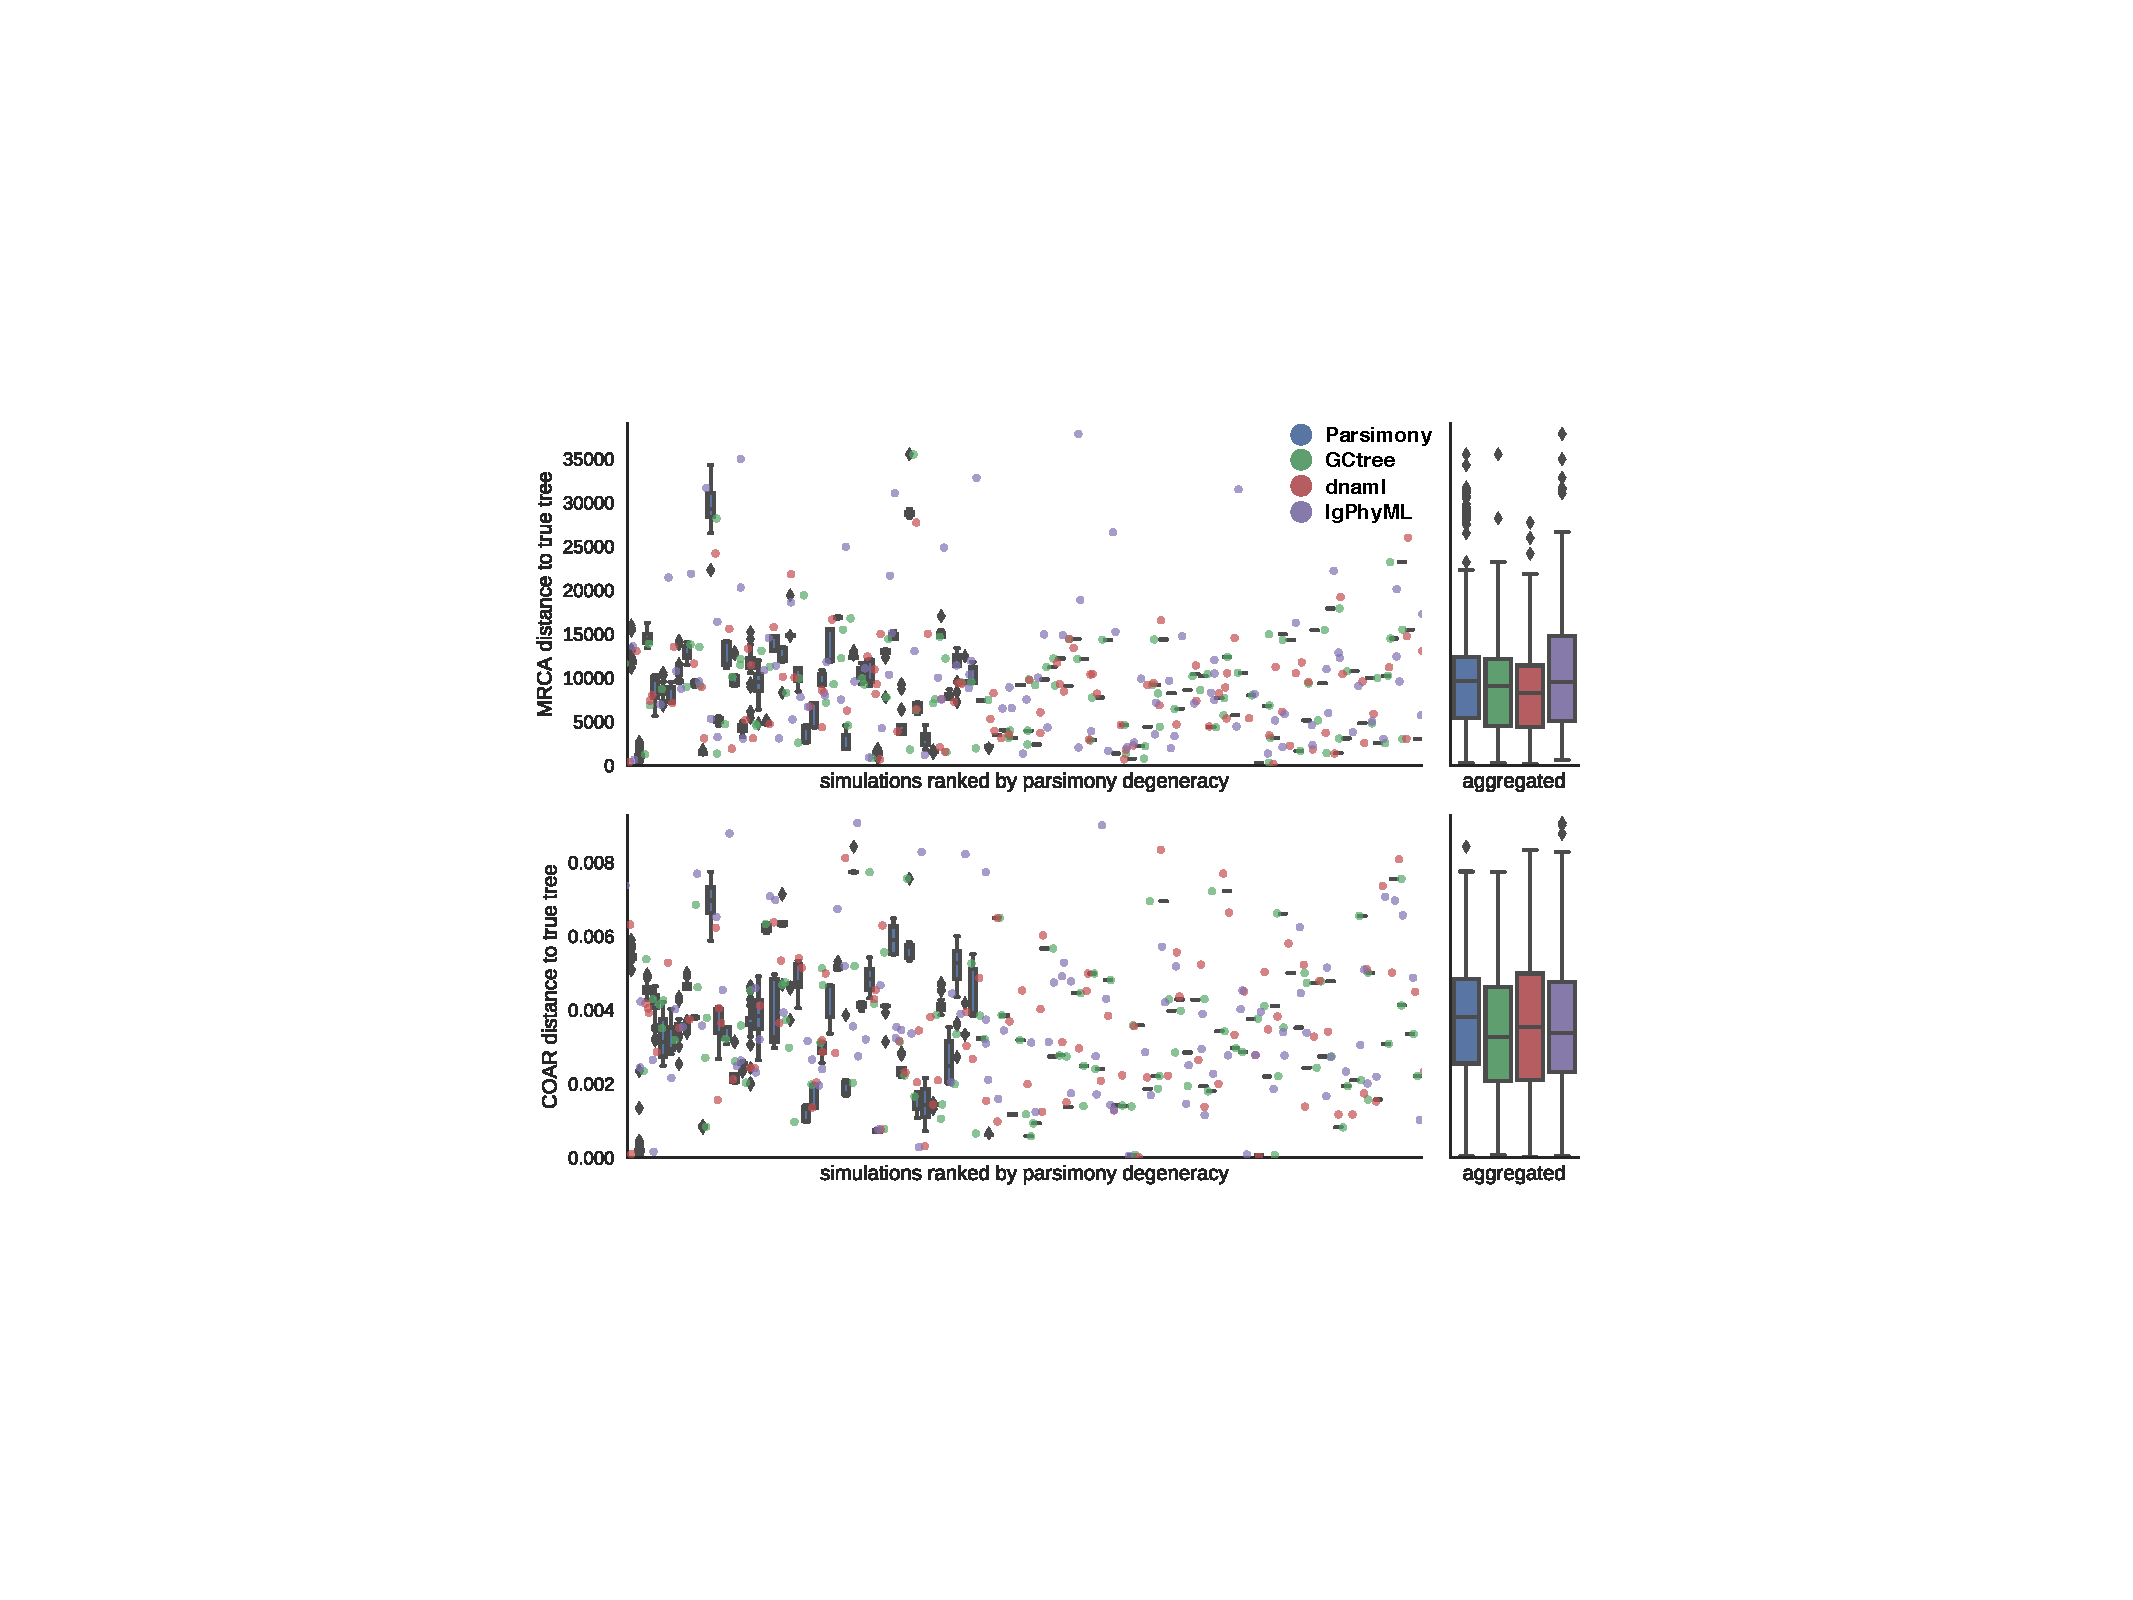
\includegraphics[width=0.9\textwidth]{figures/Laura-affsim_valid.pdf}
    \caption{
        \label{fig:Laura-affsim_valid}
        Simulation with 100 repeats of the affinity simulation.
        Each simulation is plotted in a single column ranked according to the number of equally parsimonious trees for the simulation.
        The ensemble of equally parsimonious trees are shown as a box plot while the other methods are plotted as jittered dots.
        On the right the aggregated result is shown.
    }
\end{figure}






\section{Discussion and conclusion}
Tree topology is not the biggest concern in this validation because often the topology is not a very important objective by itself.
It is the reconstructed sequences and the order of these, the selection pressure etc. that is most important.
These objectives then tend to be correlated with correct tree topology, but that does not necessarily need to be true, and therefore the main objective is to validate ASR and let the tree topology follow as a consequence of improving the ASR.

The presented COAR metric is a suitable objective for ASR since it is robust to irrelevant errors in tree topology and directly interpretable as the expected per site error of sequences in a reconstructed lineage.
The simulation study we present show that, regardless of the inference method used, the reconstruction of sequences along an ancestral lineage is robust and only rarely accumulate errors.
In a worst-case scenario there is an expected one nucleotide error per reconstructed sequence in a reconstructed lineage, based on affinity simulation with 4-8 sequences (including the a priori know root and leaf) in a lineage, see b) in figure \ref{fig:Laura-affsim_runstat} appendix B.

Simulating under a neutral branching process is not realistic compared to the fast and stringent selection process which is undertaken in the GC reaction.
The simulation with added affinity selection addresses this issue and challenges the inference methods with both epistasis and homoplasy.
Therefore it is not surprising to see that inference on affinity simulations obtain higher COAR values than neutral simulation under comparable conditions.
What is surprising is that all inference methods seems to be equally effected by the imposed affinity selection.
We would have expected a codon based model like IgPhyML to have a an advantage compared to the nucleotide based models because affinity selection is strictly on protein level, and hence there is a preference for synonymous over non-synonymous mutations that is incorporated in the model parameters of a codon model but not in a nucleotide model.
IgPhyML should also have an advantage over the other methods due to its incorporation of AID hot/cold spot motif in its model.
Although IgPhyML is marginalizing over motifs that span multiple codons, to achieve site independence, it should still capture some of the signal from mutational context bias.
Again this does not seem to improve the inference by IgPhyML over the other method.

Looking at typical trees simulated from both the neutral -and affinity selected process (see trees in appendix B) it look like trees are relatively shallow i.e. the number of internal nodes from the leaf to the root is small.
This of course makes it easier to get a low COAR score because there are only few states to reconstruct.
In the affinity model trees are simulated over a long time range but still appear shallow because cells with low affinity are lost during maturation.
On a tree this memory loss of lower affinity variants will show as a tree with a long trunk extending from the root to a bushy canopy, similar to observations made by Yaari et al. \cite{yaari2015mutation} (visualized in b) in figure \ref{fig:Laura-affsim_runstat} in appendix B).
This trait could explain why is there is no apparent benefit of integrating AID motifs into an inference algorithm like IgPhyML.

The overall performance of all the evaluated inference methods is very similar.
There is a consistent ranking that puts GCtree first, dnaml and IgPhyML second and sets Parsimony last, but it must be stressed that the difference is very small and that the performance can be regarded as practically equivalent.
GCtree that stands out as the most consistently better performing algorithm is also dependent on the genotype abundance which is not readily available for most BCR data.
Abundance data could potentially be extracted from standard HTS data but because of sequencing errors and primer biases these abundances are not reliable.
With the introduction of UMIs this problem is getting addressed and it is expected that in most future datasets that the abundance information will be more reliable, giving the opportunity to integrate abundance data in methods such as GCtree to direct phylogenetic inference.




\section{Conclusion}
The problem of inferring BCR phylogenies appears to be insensitive to the method used on the simulation regimes tested.
With a significant improvement of GCtree inference we suggest that this is used when reliable abundance information exists.
Otherwise the methods tested are practically equivalent suggesting that users should care mostly about which tool provide the most convenient solution to inferring their BCR phylogeny.
It remains to be tested whether different sampling conditions, such as time series sampling, will alter the results.
Likewise it is undetermined if joint reconstruction will do any improvement over marginal reconstruction.




\iffalse




\chapter{B cell receptor amino acid profiles}

%%%%%%% from aammp paper
Germinal center (GC) maturation is a central process of the adaptive immune system.
The Darwinian selection undertaken inside a GC is driven by B cells' ability to bind the antigen through the membrane bound B cell receptor (BCR), also known as an antibody.
The population of B cells are under stringent selection while being highly mutated, driving the cell population towards higher and higher affinity until the GC is eventually dissolved.

Each GC are though of as founded by one or a few B cells and binding just a single epitope \cite{tas2016visualizing}.
The evolutionary process is undertaken in small steps to improve the binding to this specific epitope surface and therefore it is unlikely that a switch in epitope specificity will occur.
Assuming that this holds, all cell within a clonal family will have evolved in the same context, with the objective of improving binding to the same surface as the founder cell.
Different GCs can have different epitope specificities and in these different contexts each GC will have their own fitness landscape.

When sequencing B cell repertoires it is possible to establish the clonal identity of each sequence with reasonable confidence \cite{ralph2016likelihood}, thereby relating each sequence to the GC they arose, but it is much more difficult to reconstruct the evolutionary process and the selection that happened inside the GC.
We separate selection into two classes, local and global selection.
Local selection is the context specific selection happening on all of the B cell of a single GC because they evolve towards binding the same epitope.
Local selection is therefore working on the level of epitope binding with positive selection for those mutations that confer tighter binding and vice versa.
Local selection is strictly related to binding of a single epitope surface but whether change in binding is due to direct antibody epitope contact or indirect effects improving binding by framework stabilizing or other ways, is irrelevant.
In fact the local effects capture everything we would like to estimate, there is just not sufficient data to do so and therefore we turn to global effects.
Global effects on selection are the subset of local effects shared between clonal families.
These will be different from direct binding effects and typically reflect conservation of general antibody features such as frame work beta sheet interactions and protein stability.
Analysis of global effect in a large repertoire was recently undertaken by McCoy et al.\ where it was found that selection was correlated with surface exposure of a residue \cite{mccoy2015quantifying}.
This might be an indirect effect related to the correlation between surface exposure of a residue and its effect on protein stability \cite{echave2016causes}.

In the selection process some mutations will increase the BCR affinity and eventually be fixed, while some might be deleterious and counter selected, and finally some are just neutral accumulating throughout the evolution.
This can be expressed in the terms of a observation probability vector for each position, where the probability of is observing a given amino acid is proportional to the fitness of that amino acid vs.
the other 19 possible substitutions.
Raw counts of amino acids over each site will at the limit of an infinite number of sequence observations correspond to the true vector of probabilities however due to the limited number of sequences occurring in a GC, raw counts is not a good estimator.
Therefore it is necessary to enforce the estimate of selection within a single GC with information derived from similar GCs.
In this scheme the local context specific effects will be combined with global information derived from many more sequences from related GCs by using the global effects as prior information feeding into the selection estimate on local scale.

While germinal center phylogenetic reconstruction is highly informed by nucleotide sequences, selection is working on protein sequences and synonymous codons, coding the same amino acid, does not possess any fitness advantage.
The functional form of the BCR is a protein and therefore the purpose of our model is the describe the selection on codon level.
Furthermore the codon level of selection is of increasing interest due to the potential use in engineering antibodies for human disease therapy like cancer, acute infections, auto-immune disease and rare genetic disease.

In this article we are suggesting a new approach to leverage global constraints on the BCR protein sequence across different epitope contexts with local information of sequences sharing the same epitope context.
Using this model it is possible to find the conserved sites and most likely allowed substitutions, useful in antibody engineering while keeping the target epitope conserved.


%%%%%%










Bla bla introduction
This can be used for bla


Observed BCR sequences does not necessarily have therapeutic potential e.g. B cell don't care about aggregation and viscosity, and probably doesn't care much about heat stability and pH tolerance either.
What observed BCR sequences really provide is a lower bound on what can be a therapeutic antibody i.e. if an antibody cannot be functional in a B cell it will never get to be a therapeutic antibody, but just because it has been observed it does not mean that it have full potential to as a therapeutic antibody.



\section{Model description}
%Amrit has a small section on a math description of aammp:
Maybe insert math description:
\url{https://www.overleaf.com/8548257cyshmbtrkywn#/30398139/}




Simulation of expected substitution profile given the naive sequence, mutation burden and motif model.








\fi


\chapter{Perspectives}
Understanding the mechanisms of BCR evolution in GCs is one of the most fundamental topics in the research area of adaptive immunity.
The ability of the human body to produce high affinity antibodies has profound implications in human medicine, immediately apparent by their role in preventing bacterial and viral infections through vaccines or previous exposure, but also through the role of auto-antibodies in autoimmune diseases, with pemphigus vulgaris \cite{payne2005genetic} myasthenia gravis \cite{lindstrom1998antibody} and rheumatoid arthritis \cite{steiner2002autoantibodies} being just a few examples.
Not only will better understanding of GC evolution be an advancement in human molecular physiology but, maybe even more so, an important step towards taking advantage of mechanistic understanding of adaptive immunity to engineer better vaccines, the next cancer drug or treatments of autoimmune diseases.

Phylogenetic inference plays an important role in the study of BCR evolution.
Used correctly, phylogenetic inference is a strong tool offering a large body of ordered information directly useful as an engineering tool or to create new hypotheses to be scrutinized by experimental studies.
On the other hand phylogenetic inference can also be misused by over-emphasizing its importance, neglecting the uncertainties involved in the inference or just by plain misunderstanding.
With the recent technological advances of HTS the possibilities of studying BCR evolution has expanded into new dimensions, and with this have followed an increasing interest in applying phylogenetic tools to study everything from vaccine responses \cite{raymond2016influenza}, to development of broadly neutralizing antibodies (bnAbs) targeting HIV \cite{Doria-Rose2014-vi}, \cite{Wu2011-yj}, \cite{Zhu_undated-zz} and influenza \cite{pappas2014rapid}, \cite{xu2015key} and even in studying the repertoire effects of aging \cite{de2017phylogenetic}.
ASR has been used to reveal that one of the barriers for eliciting bnAbs towards HIV is that they tend to evolve from self-reactive naive sequences \cite{williams2017potent}, \cite{liao2011initial}, thereby making it less likely for possible bnAb precursors to receive T cell help to found and sustain a GC.

In the last decade development of therapeutic antibodies has boomed, with at least 47 FDA approved and marketed antibodies and growing number of approvals \cite{ecker2015therapeutic} the market for antibodies has never been stronger.
Most antibodies derive from animal immunization or human PBMC isolation \cite{reichert2012marketed} and are therefore a direct outcome of GC affinity maturation.
In such instances the evolutionary history of a antibody can be of tremendous interest due to its application in antibody engineering.
Suppose the phylogenetic tree of the GC maturation can be reconstructed, this will provide a wealth of information about sequence conservation and relationship to other sequences with the same antigen binding site, information that can be applied in engineering and optimization which is a bottleneck in the antibody discovery phase \cite{dubel2014handbook}.
Phylogenetic method are therefore important across the board, from basic research to pure sequence engineering.

In this work we have defined a novel way of comparing ASR using an alignment of reconstructed lineages and normalizing to a per-site expected error.
%EM I feel like the original motivation for COAR, namely that we are interested in the expected error in reconstructing lineage leading to a particular sequence which has been identified using lab work, could be greater emphasized here and in the COAR introduction.
We call this the COAR metric, and it is especially useful for assessing the ASR performance of different phylogenetic inference method on simulated data.
For simulation of sequences on a fixed tree ASR performance can readily be evaluated by comparing equivalent nodes, as done by Hoehn et al.\ \cite{Hoehn2016-wg}, however when the tree itself is also being simulated e.g.\ by a stochastic branching processes, then the comparison becomes less trivial.
COAR provides a way of producing comparable ASR benchmark values regardless of the simulation methods used and we hope that this will be useful in future work of ASR validation.

To validate different inference methods we also created a framework for simulating trees by a stochastic branching process using an SHM biased mutation process.
To simulate the Darwinian selection occurring in the GC maturation we couple a branching process simulation with affinity based selection acting on individual sequences.
Using COAR and other validation metrics we have run extensive validation studies and shown that a variety of phylogenetic inference is robust and accurately reconstructs ancestral sequences.
The validation also showed that incorporation of sequence metadata like abundances can significantly increase the performance of ASR.
IgPhyML, which is the only method to explicitly model the context sensitive mutation process of SHM, did to our surprise not perform better than the other methods.
We speculate that there is there is not enough signal from the SHM bias due to the relatively shallow trees, including the fact that IgPhyML is using a mean field approximation which is prone to averaging out large parts of signal embedded in the sequence motifs.
Unfortunately this mean field approximation is necessary to achieve site independence and making a tractable likelihood evaluation and therefore the problem is not easily solved by a modification to the model.

In future iterations of this validation we would like to investigate in more detail whether SHM motifs can be integrated in other ways into the inference algorithm and then search for situations where this might add significant value.
We are currently working on using motif information in a similar way as abundance information is used in GCtree i.e.\ calculating the likelihood of a tree given a motif model and then ranking a set of equally parsimonious trees according to their motif based likelihood.
It is also possible for us to avoid the problem of shallow trees by sampling multiple time points during the simulated GC evolution, and in addition to solving that problem it will answers essential questions about the validity of BCR phylogenies inferred on PBMC samples drawn at different stages of an immunization.
Inferring phylogenies from a time series of samples could be an interesting way of exploring the evolutionary trajectories of an immunization in the future.

There will always be a question about just how realistic sequence simulations are, whether they are too easy, bias or not capturing the traits of real GC evolution.
We have presented two alternative approaches to simulate GC evolution and shown that these represent varying degrees of difficulties for inference methods, however we imagine that the affinity selection model could be even more challenging by drawing target affinities and "distance to affinity" conversion steepnesses ($k$ in \eqref{eq:hd2affy}) from a distribution rather than having a single value for all targets.
Alternatively a much more detailed mechanistic model could be used for affinity simulations.
Unfortunately, methods like hyphasma \cite{robert2017simulate} does not support simulation of BCR sequences but it does integrate a string comparison method as a proxy for affinity.
It appears to be possible that the explicit DNA representation of BCR sequences described in our affinity simulation could be transferred into the larger framework of hyphasma, thereby enabling sequence simulation from a high level mechanistic model.
Lastly it is also possible that we can improve simulations further by adjusting simulation parameters to fit more characteristic behaviours found in real datasets.
One example would be to use the MP tree degeneracy as another metric for the simulated sequences to recapitulate.
With the big interest in germinal center biology and increasing technical advances, we expect soon to see more single GC datasets like the one from Tas et al.\ \cite{tas2016visualizing}.
Such datasets might even contain information like antigen affinities which could be used to adjust our affinity simulation at the same time as being excellent experimental data to recapitulate in a simulation.



\appendix
\chapter{Tables}

\begin{table}[!ht]
\centering
\begin{tabular}{|l|l|l|l|l|l|l|}
\hline
 & \multicolumn{2}{c|}{COAR}                             & \multicolumn{2}{c|}{MRCA}                             & \multicolumn{2}{c|}{RF}                               \\ \hline
                 & \multicolumn{1}{c|}{Mean} & \multicolumn{1}{c|}{STDV} & \multicolumn{1}{c|}{Mean} & \multicolumn{1}{c|}{STDV} & \multicolumn{1}{c|}{Mean} & \multicolumn{1}{c|}{STDV} \\ \hline
Parsimony        & 1.67E-04                  & 2.32E-04                  & 38.6                      & 65.2                      & 3.59                      & 2.40                      \\ \hline
GCtree           & 7.57E-05                  & 2.01E-04                  & 26.1                      & 84.0                      & 1.46                      & 1.87                      \\ \hline
dnaml            & 2.01E-05                  & 9.08E-05                  & 30.9                      & 103                       & 0.49                      & 0.98                      \\ \hline
IgPhyML          & 9.95E-05                  & 1.74E-04                  & 35.0                      & 101                       & 2.39                      & 2.02                      \\ \hline
\end{tabular}
\caption{
\label{tab:Tas-neutsim_vali}
Mean and standard deviation (STDV) for 100 simulations under the neutral model fitted to the Tas. dataset. Plotted in \ref{fig:Tas-neutsim_vali}.
}
\end{table}


\begin{table}[!ht]
\centering
\begin{tabular}{|l|l|l|l|l|l|l|}
\hline
 & \multicolumn{2}{c|}{COAR}                             & \multicolumn{2}{c|}{MRCA}                             & \multicolumn{2}{c|}{RF}                               \\ \hline
                & \multicolumn{1}{c|}{Mean} & \multicolumn{1}{c|}{STDV} & \multicolumn{1}{c|}{Mean} & \multicolumn{1}{c|}{STDV} & \multicolumn{1}{c|}{Mean} & \multicolumn{1}{c|}{STDV} \\ \hline
Parsimony       & 1.93E-04                  & 2.03E-04                  & 1116                      & 1804                      & 13.0                      & 7.04                      \\ \hline
GCtree          & 1.76E-04                  & 2.23E-04                  & 577                       & 1229                      & 8.96                      & 7.22                      \\ \hline
dnaml           & 2.37E-04                  & 4.34E-04                  & 602                       & 1415                      & 8.6                       & 6.6                       \\ \hline
IgPhyML         & 2.29E-04                  & 2.31E-04                  & 873                       & 1832                      & 7.69                      & 6.14                      \\ \hline
\end{tabular}
\caption{
\label{tab:Laura-neutsim_vali}
Mean and standard deviation (STDV) for 100 simulations under the neutral model fitted to HTS data. Plotted in \ref{fig:Laura-neutsim_vali}.
}
\end{table}









\begin{table}[!ht]
\centering
\begin{tabular}{|l|l|l|l|l|}
\hline
 & \multicolumn{2}{c|}{COAR}                             & \multicolumn{2}{c|}{MRCA}                             \\ \hline
                 & \multicolumn{1}{c|}{Mean} & \multicolumn{1}{c|}{STDV} & \multicolumn{1}{c|}{Mean} & \multicolumn{1}{c|}{STDV} \\ \hline
Parsimony        & 8.62E-04                  & 1.10E-03                  & 310                       & 189                       \\ \hline
GCtree           & 7.34E-04                  & 9.06E-04                  & 274                       & 277                       \\ \hline
dnaml            & 6.21E-04                  & 8.89E-04                  & 185                       & 193                       \\ \hline
IgPhyML          & 7.12E-04                  & 8.93E-04                  & 280                       & 228                       \\ \hline
\end{tabular}
\caption{
\label{tab:Tas-affsim_vali}
Mean and standard deviation (STDV) for 100 simulations under the affinity model fitted to the Tas. dataset. Plotted in \ref{fig:Tas-affsim_vali}.
}
\end{table}


\begin{table}[!ht]
\centering
\begin{tabular}{|l|l|l|l|l|}
\hline
 & \multicolumn{2}{c|}{COAR}                             & \multicolumn{2}{c|}{MRCA}                             \\ \hline
                 & \multicolumn{1}{c|}{Mean} & \multicolumn{1}{c|}{STDV} & \multicolumn{1}{c|}{Mean} & \multicolumn{1}{c|}{STDV} \\ \hline
Parsimony        & 3.66E-03                  & 1.70E-03                  & 9770                      & 5838                      \\ \hline
GCtree           & 3.44E-03                  & 1.79E-03                  & 8899                      & 5848                      \\ \hline
dnaml            & 3.64E-03                  & 1.99E-03                  & 8648                      & 5497                      \\ \hline
IgPhyML          & 3.74E-03                  & 2.09E-03                  & 11055                     & 8271                      \\ \hline
\end{tabular}
\caption{
\label{tab:Laura-affsim_vali}
Mean and standard deviation (STDV) for 100 simulations under the affinity model fitted to HTS data. Plotted in \ref{fig:Laura-affsim_vali}.
}
\end{table}






\vfill
\clearpage
\newpage

\chapter{Figures}



\section{Affinity simulation trees with stats}
\begin{figure}[!ht]
    \centering
    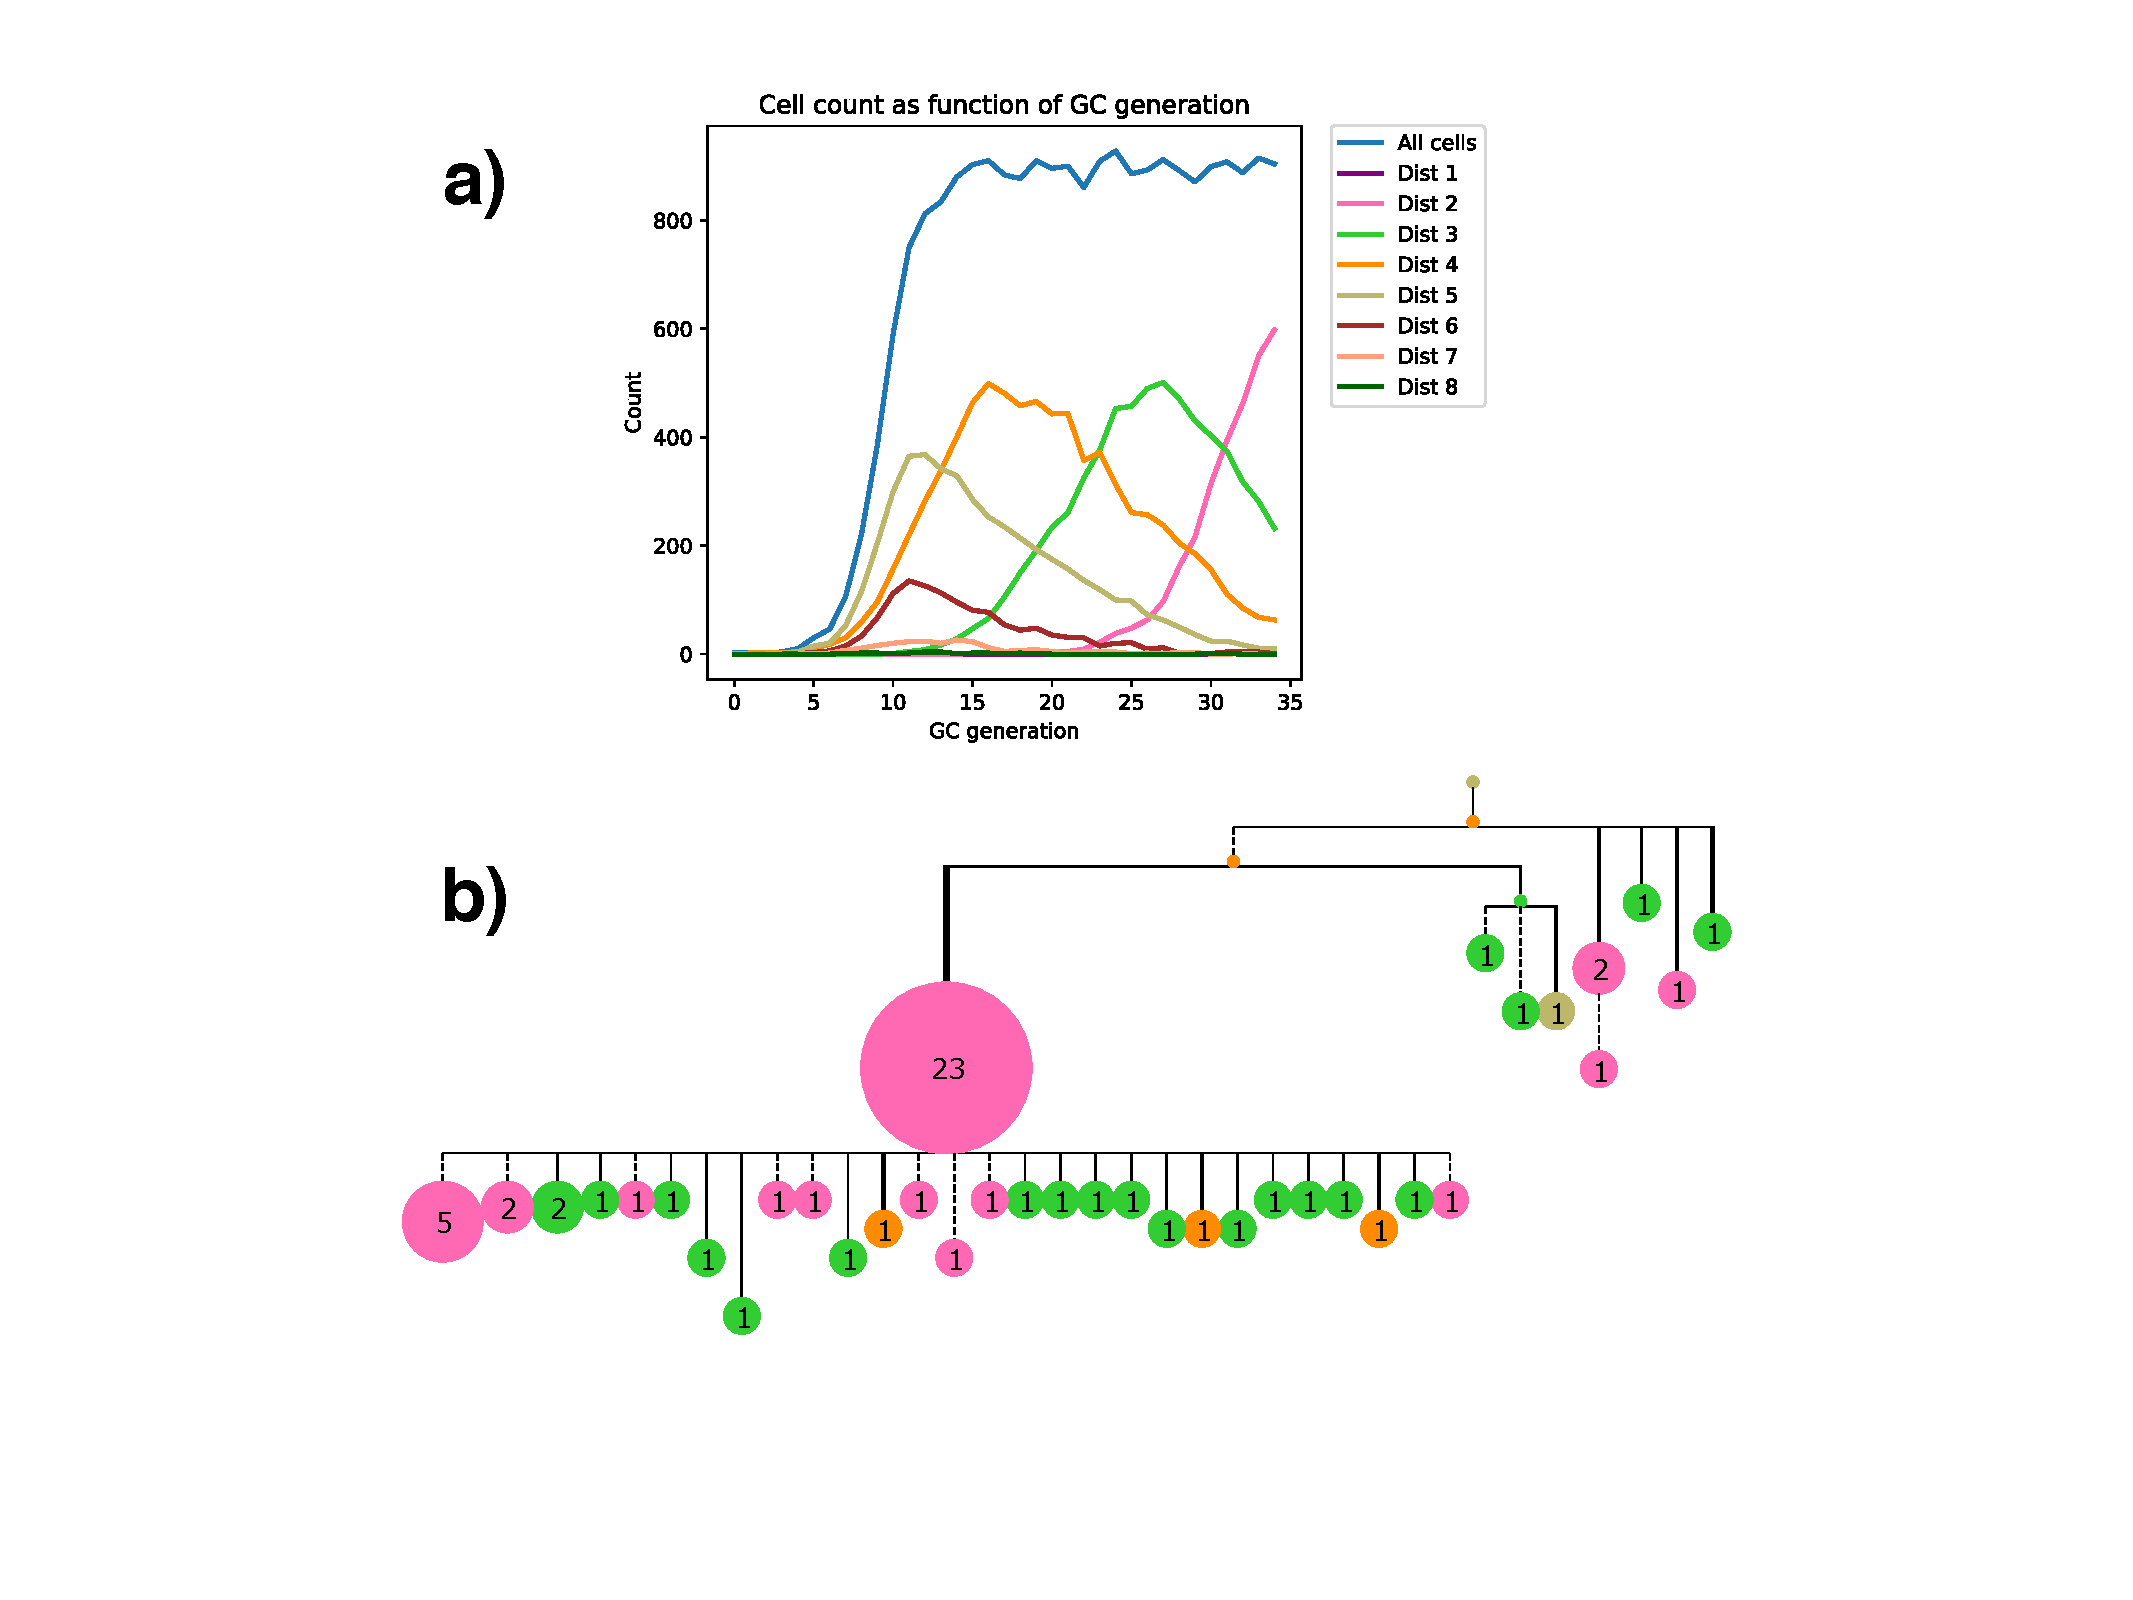
\includegraphics[width=0.8\textwidth]{figures/Tas_affsim_example_with_runstats.pdf}
    \caption{
        \label{fig:Tas_affsim_example_with_runstats}
        Summary statistics for the simulation similar to a single cell GC in figure \ref{fig:Tas_affsim_example.collapsed_runstat_color_tree}. a) run stats with color codes corresponding to affinity (through smallest distance to a target), b) resulting tree with colors matching those in a).
    }
\end{figure}





\section{Affinity simulation with visual epistasis}
\begin{figure}[!ht]
    \textbf{(a)}
    \vspace{-15mm}
    \begin{center}
    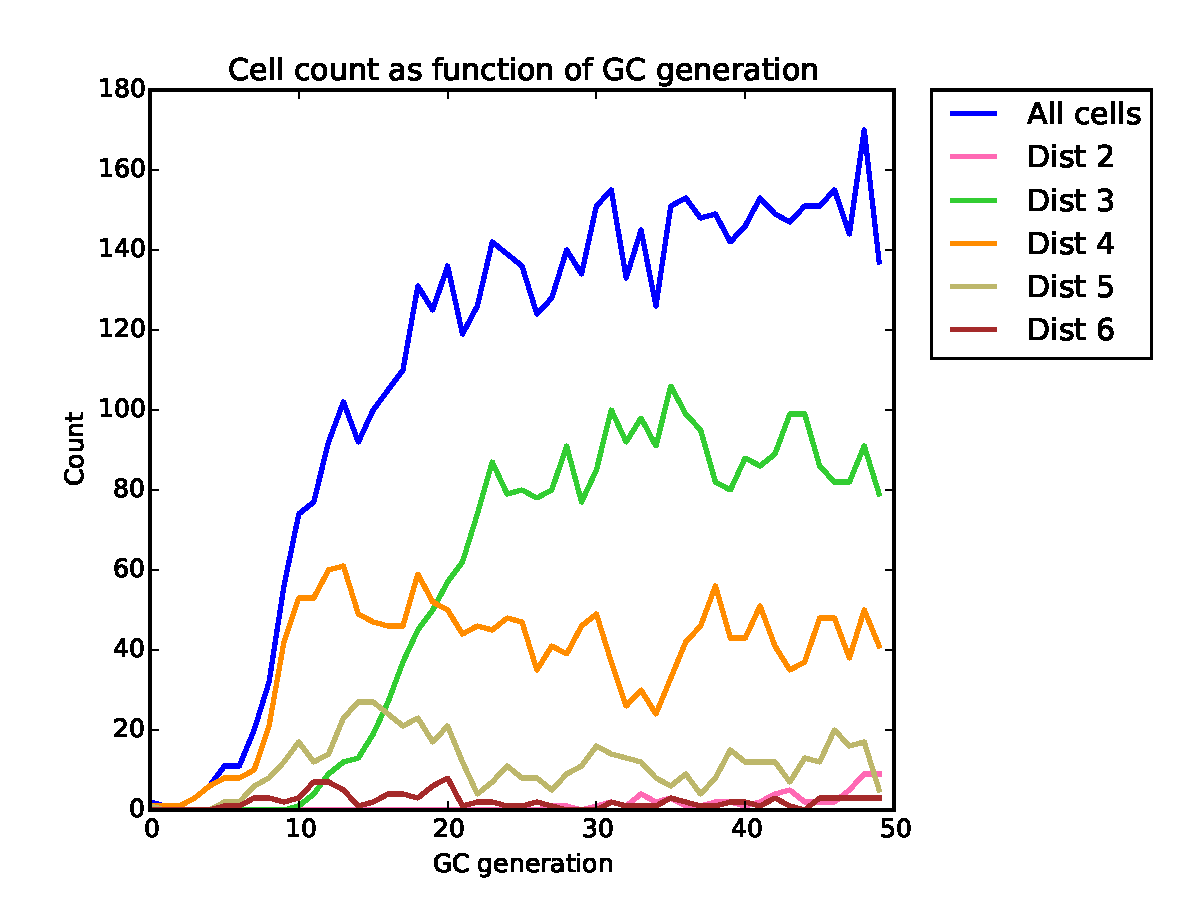
\includegraphics[width=0.6\textwidth]{figures/epi_runstats.pdf}
    \end{center}
    \textbf{(b)}
    \vspace{-15mm}
    \begin{center}
    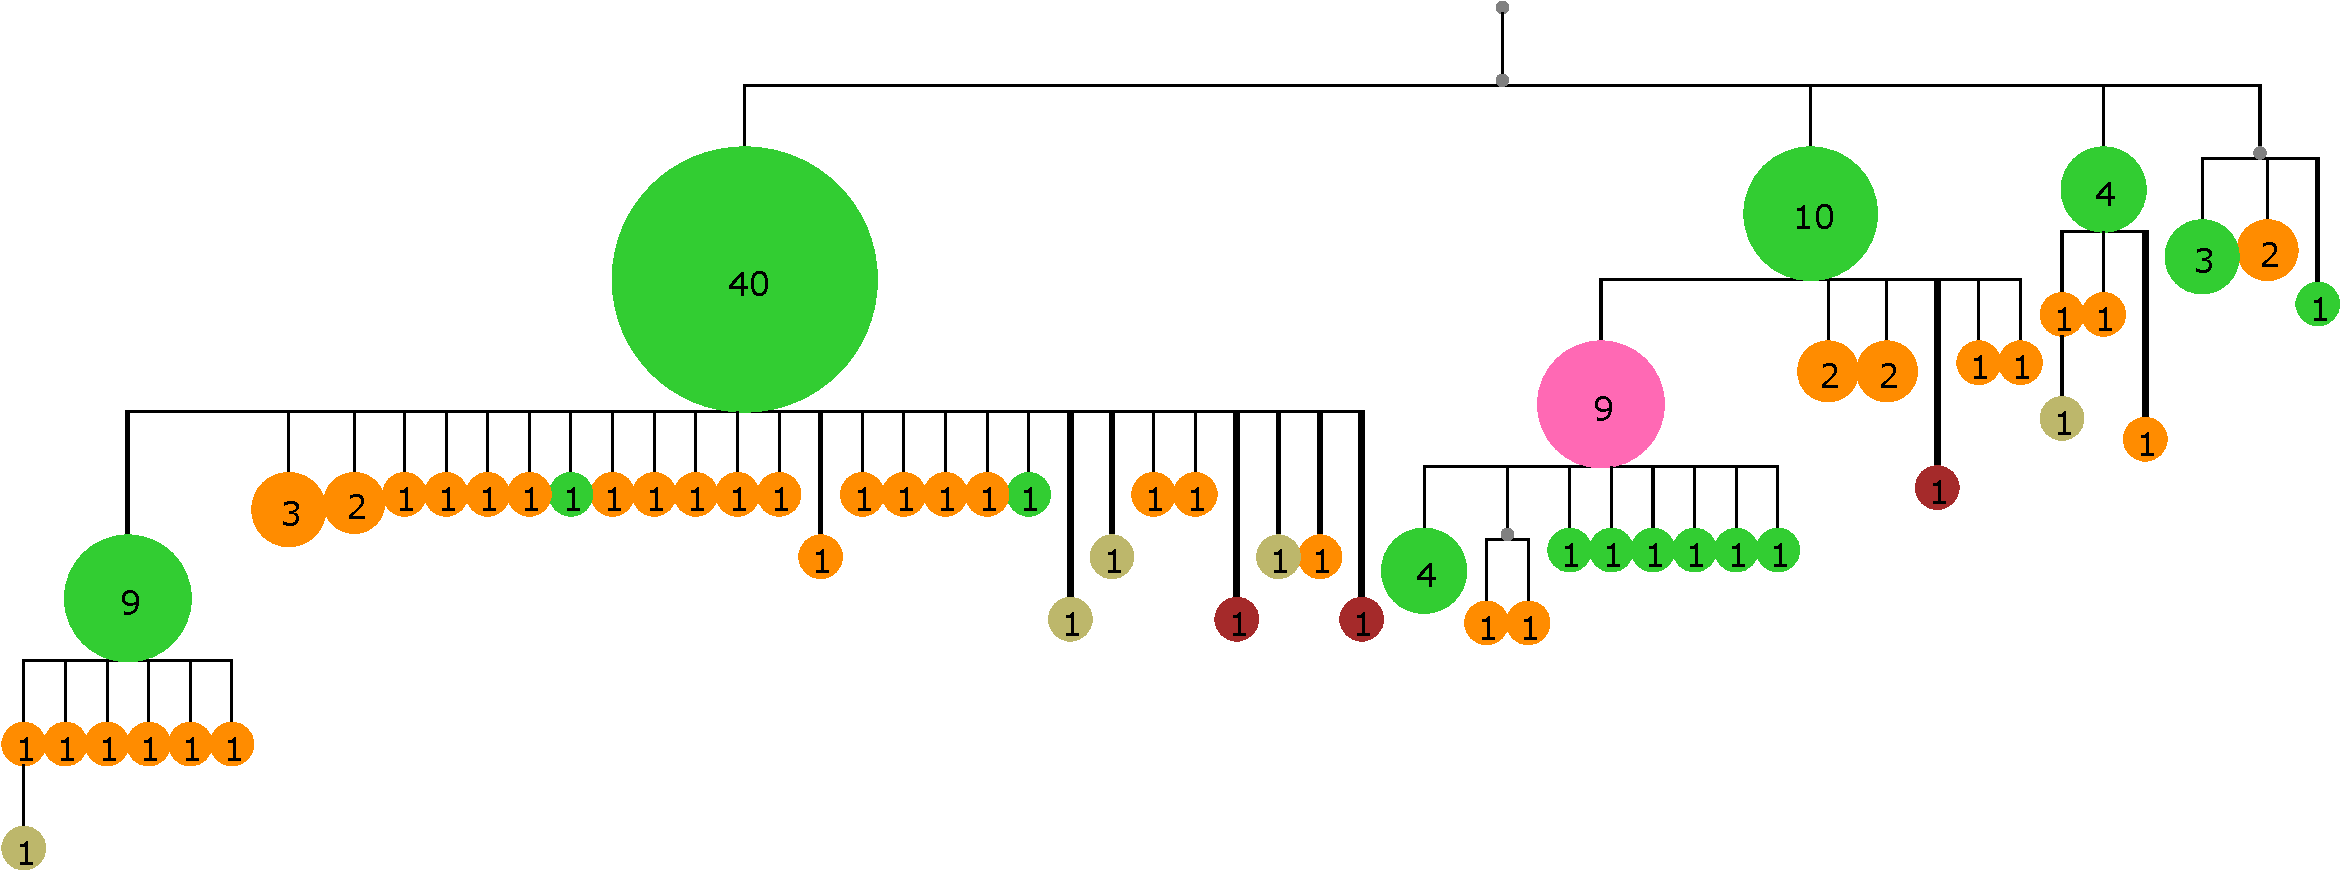
\includegraphics[width=1\textwidth]{figures/epi_collapsed_tree_runstats.pdf}
    \end{center}
    \caption{
        \label{fig:collapsed_epistasis}
        Summary statistics for the simulation showing switch in target sequences trajectories described in figure \ref{fig:epistasis_figure}. a) run stats, b) resulting tree.
        }
\end{figure}




%\iffalse


\clearpage
\section{Simulation comparison to data}
% Laura-neutsim_Laura-data
% Laura-neutsim_Tas-data   %%% Supp.

% Laura-affsim_Laura-data
% Laura-affsim_Tas-data   %%% Supp.

% Tas-neutsim_Laura-data   %%% Supp.
% Tas-neutsim_Tas-data

% Tas-affsim_Laura-data   %%% Supp.
% Tas-affsim_Tas-data

% Laura data should be referred to as HTS data
% The Tas data will be referred to as single cell data


\begin{figure}[!ht]
    \centering
    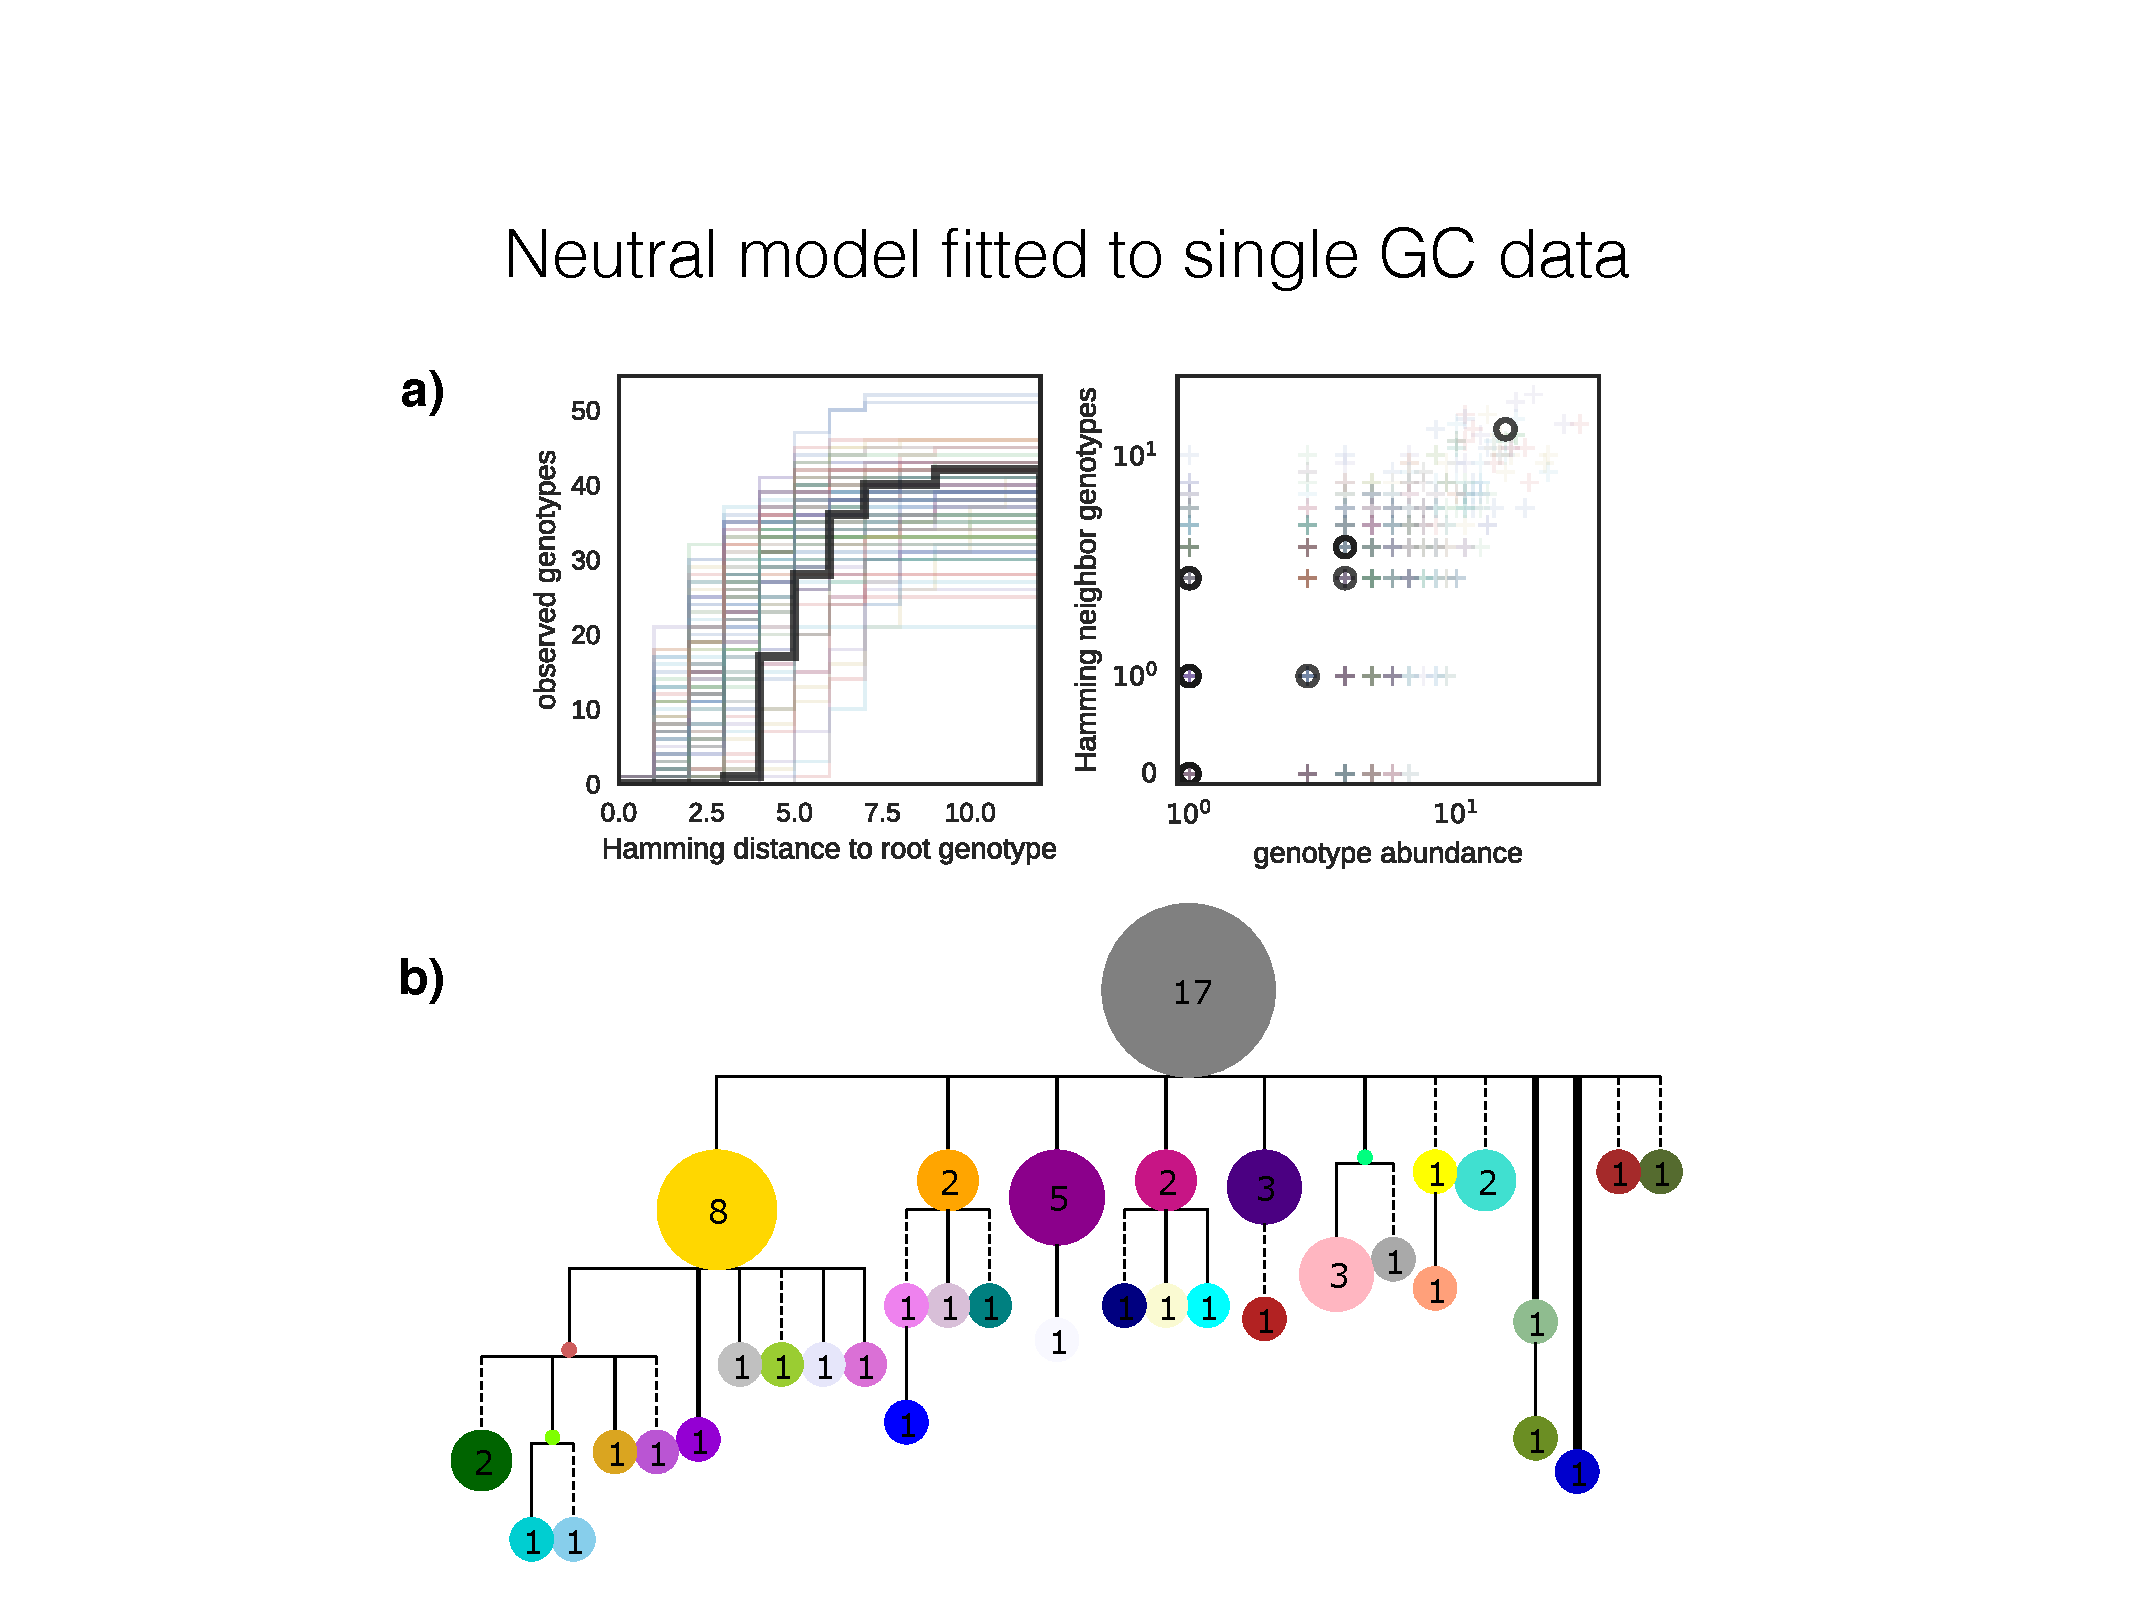
\includegraphics[width=0.8\textwidth]{figures/Tas-neutsim_runstat.pdf}
    \caption{
        \label{fig:Tas-neutsim_runstat}
        Neutral branching process with parameters fit to single cell data. In a) summary statistics of how well the simulations fit data (simulation in colors, data in black). In b) a typical tree topology from the simulation run.
    }
\end{figure}
\begin{figure}[!ht]
    \centering
    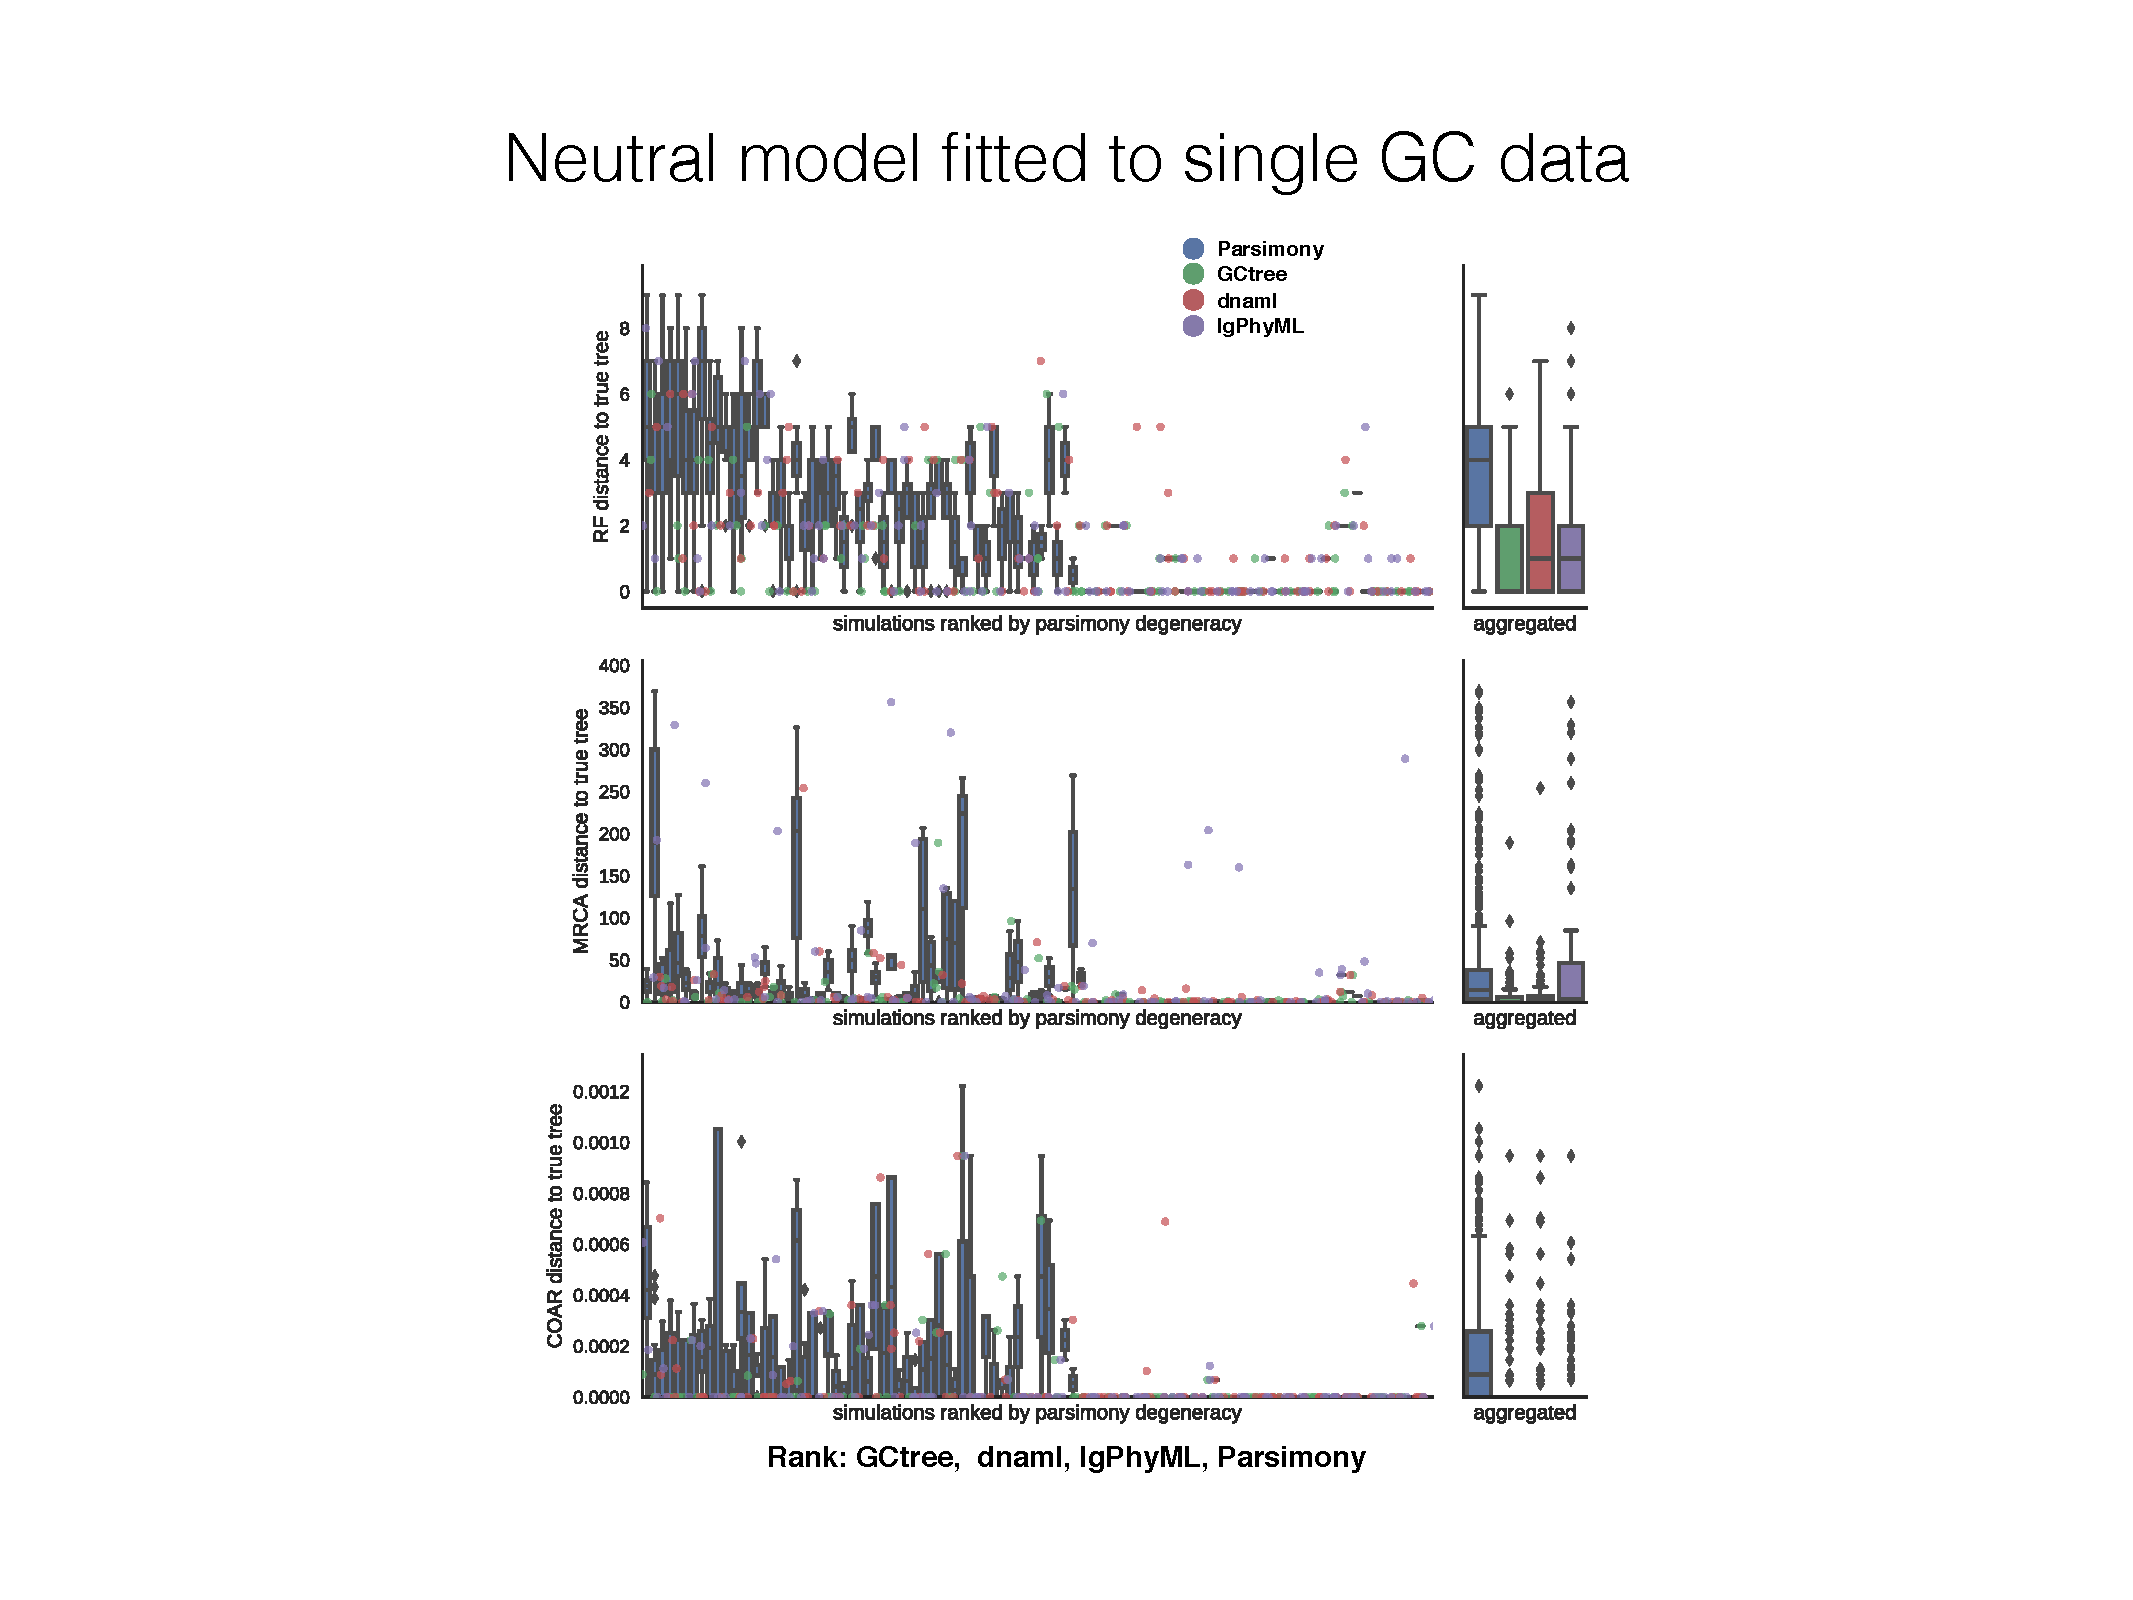
\includegraphics[width=0.8\textwidth]{figures/Tas-neutsim_vali.pdf}
    \caption{
        \label{fig:Tas-neutsim_vali}
        Performance of different inference method over the 100 simulations shown in \ref{fig:Tas-neutsim_runstat}.
        Standard box plot format with the box covering the two middle quartiles (Q2=25\% to Q3=75\% percentile), whiskers extends these and extra 1.5 times the interquartile range and points outside this are plotted individually.
        The median is indicated by a black line.
        A rank of best to worst, is subjectively decided based on the metrics plotted and with importance of the metrics determined by the rank; COAR, MRCA, RF.
    }
\end{figure}

\begin{figure}[!ht]
    \centering
    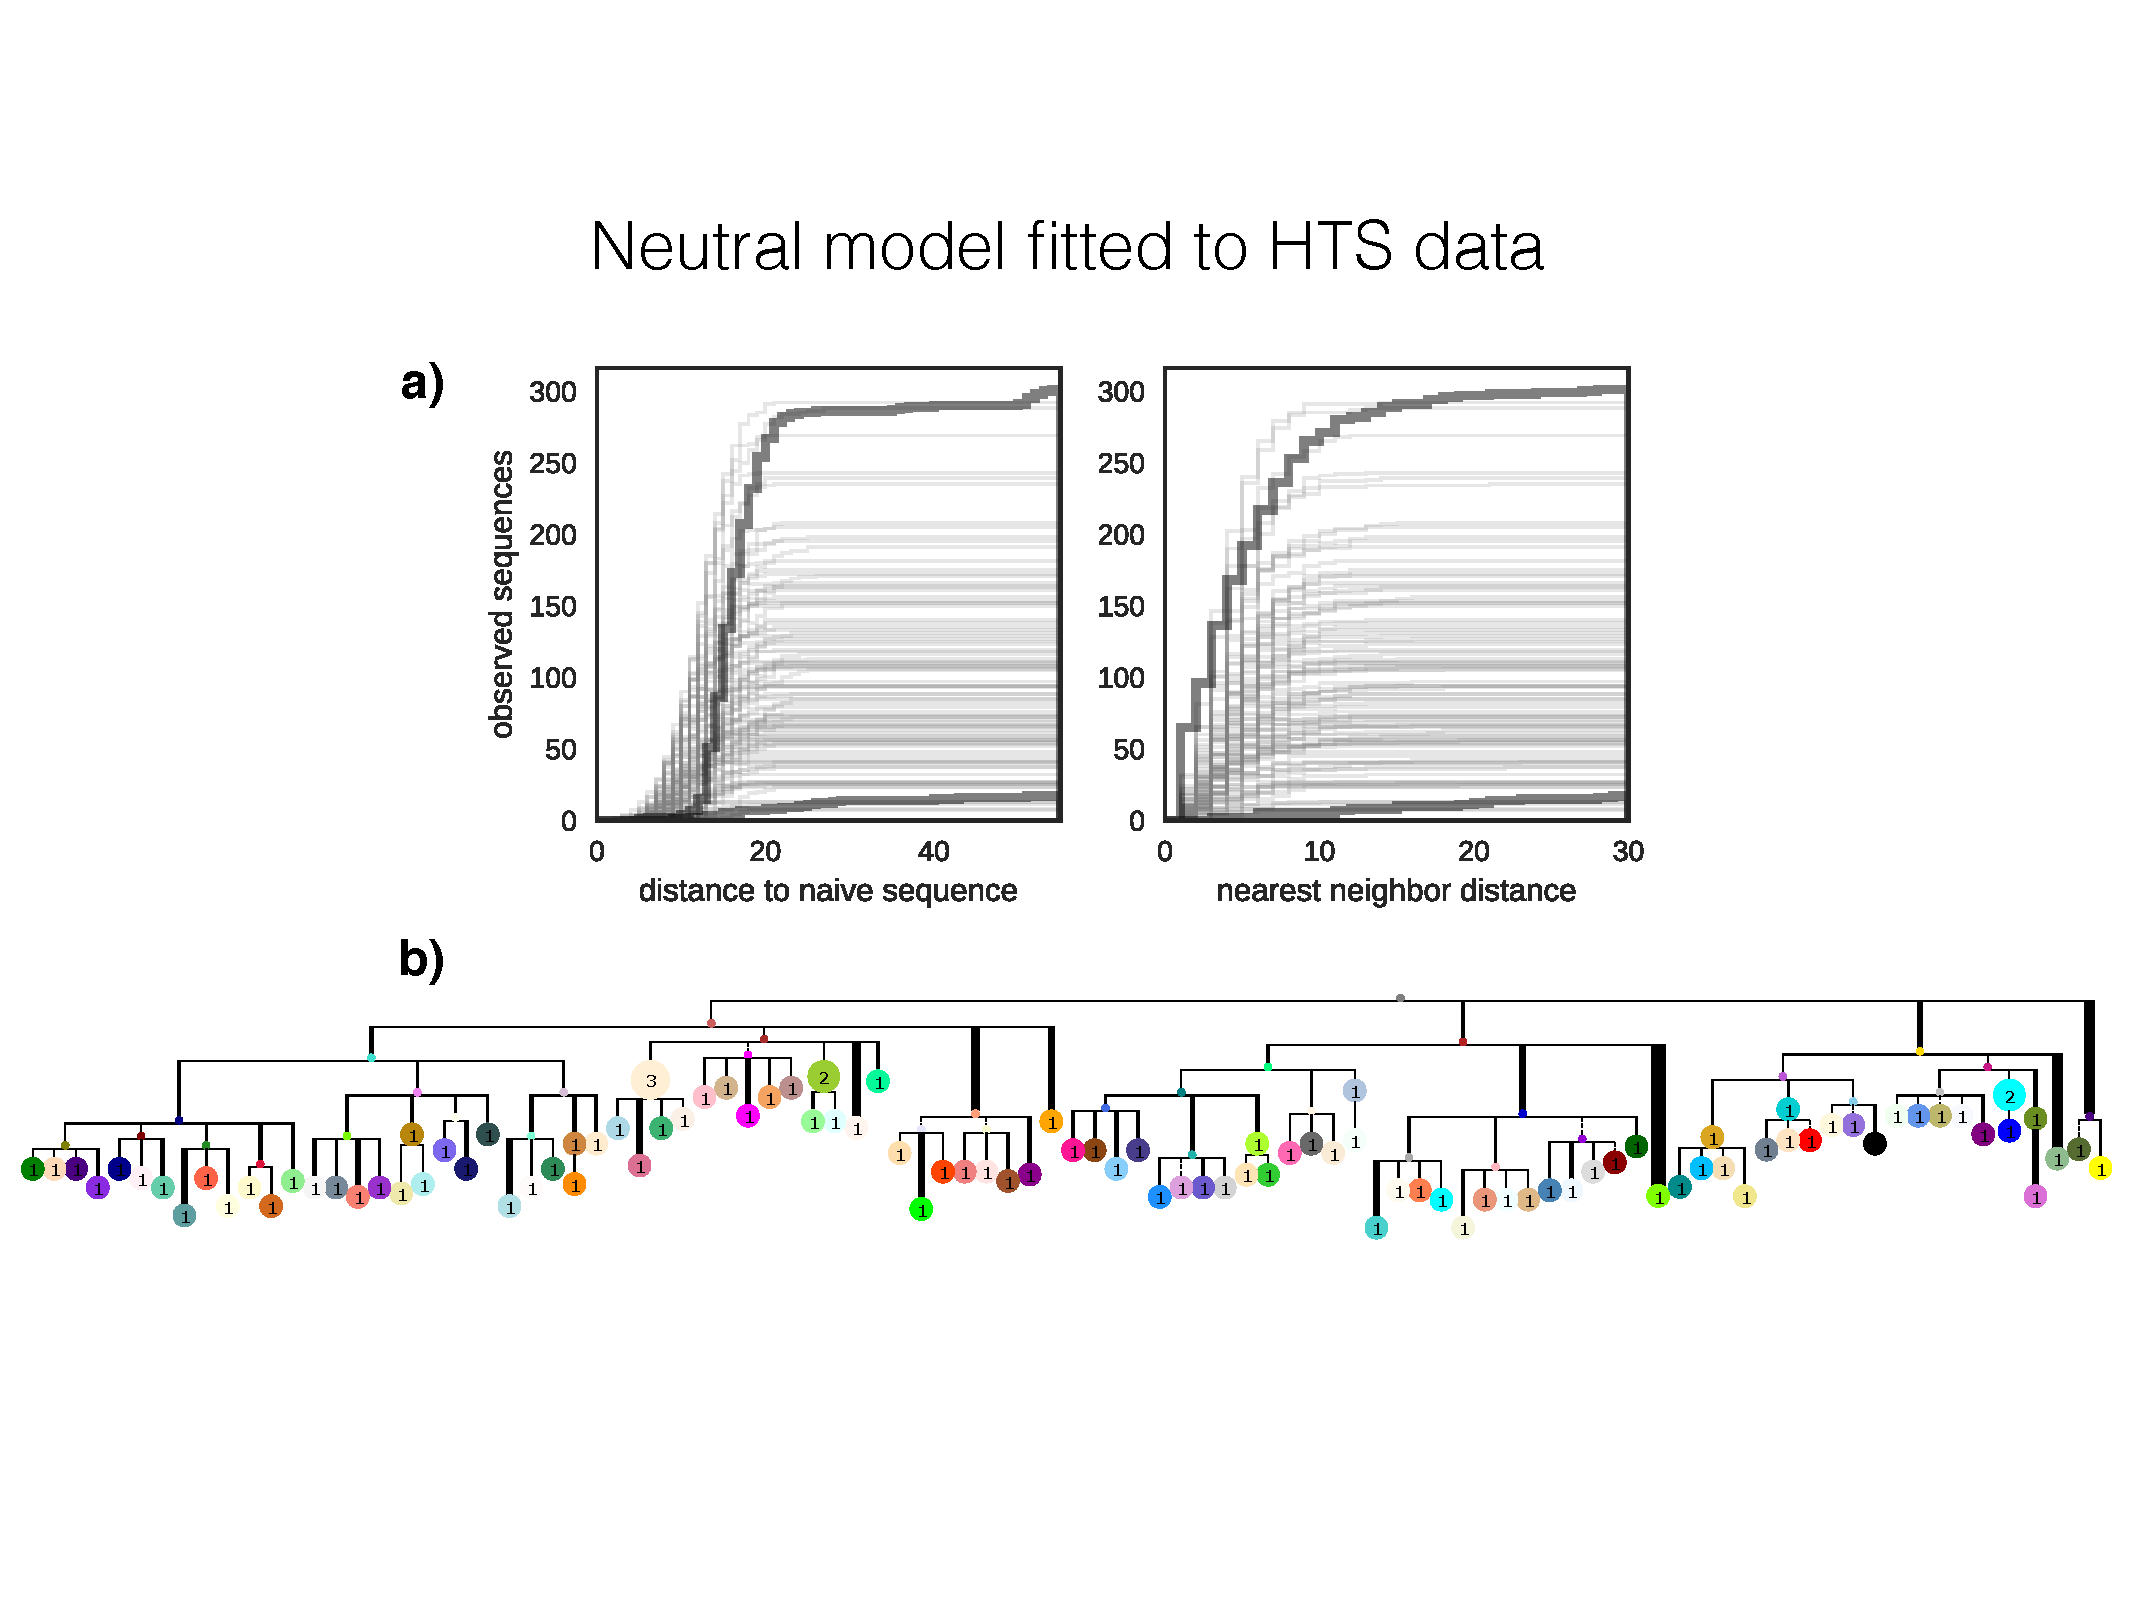
\includegraphics[width=1\textwidth]{figures/Laura-neutsim_runstat.pdf}
    \caption{
        \label{fig:Laura-neutsim_runstat}
        Neutral branching process with parameters fit to HTS data. In a) summary statistics of how well the simulations fit data (simulations in grey shade, data in dark grey). In b) a typical tree topology from the simulation run.
    }
\end{figure}
\begin{figure}
    \centering
    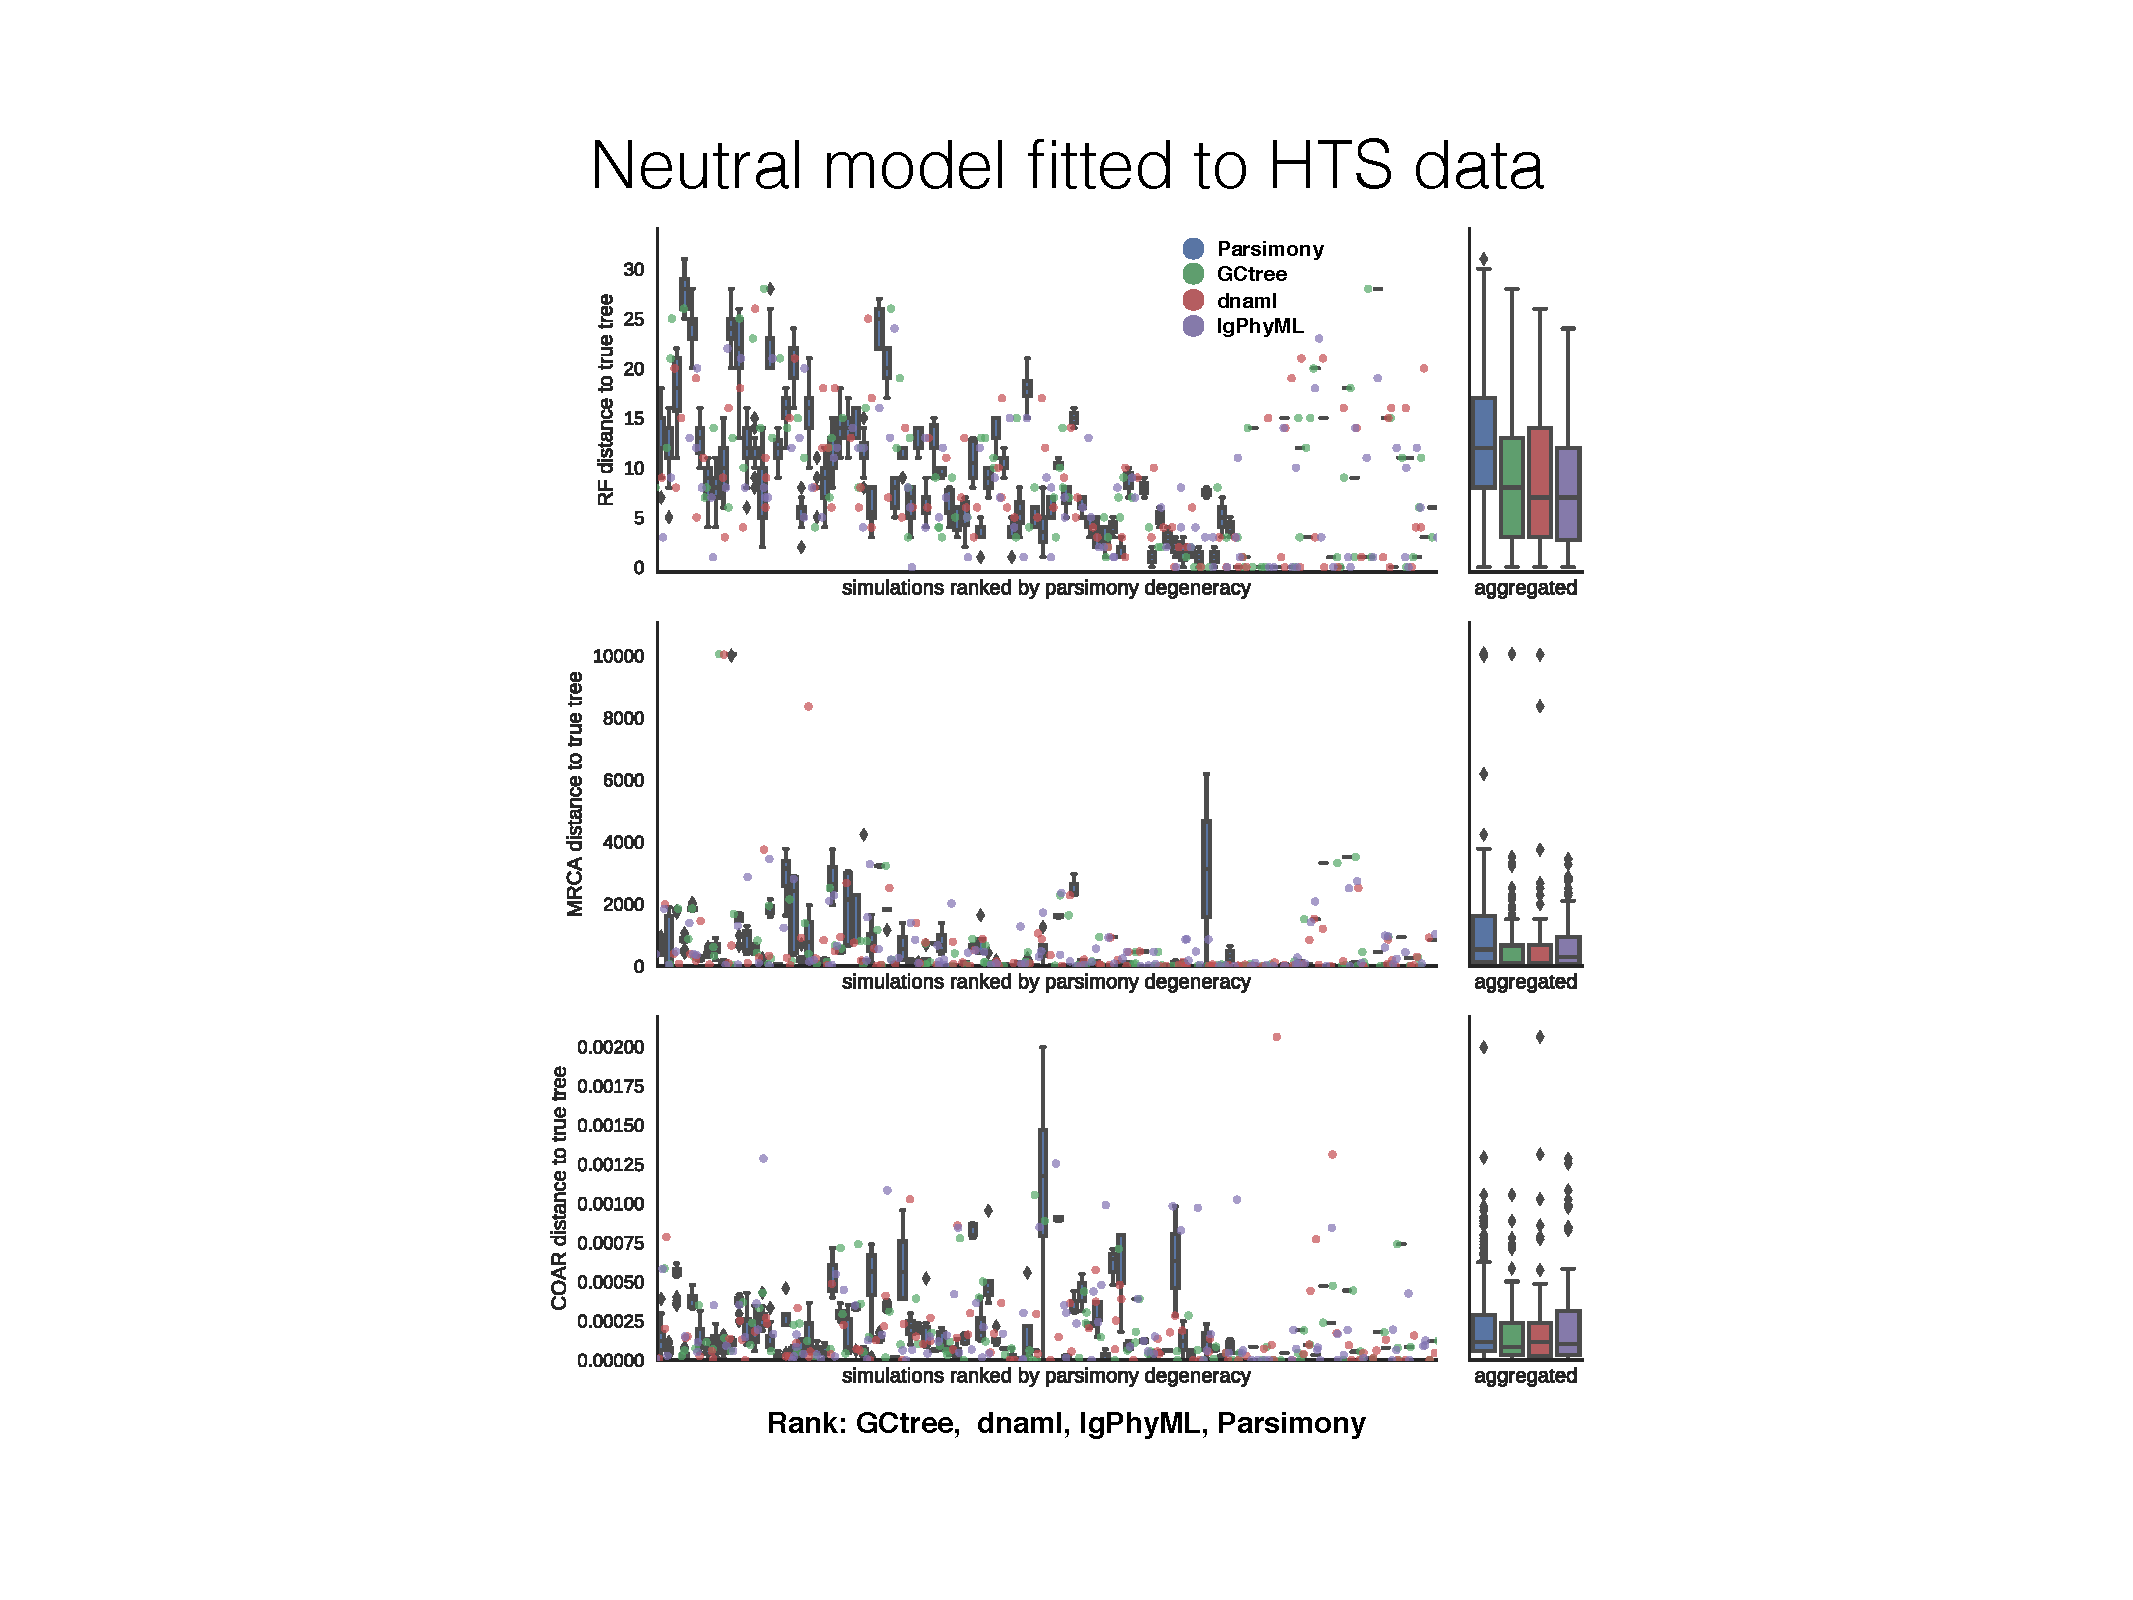
\includegraphics[width=0.8\textwidth]{figures/Laura-neutsim_vali.pdf}
    \caption{
        \label{fig:Laura-neutsim_vali}
        Performance of different inference method over the 100 simulations shown in \ref{fig:Laura-neutsim_runstat}.
        Standard box plot format with the box covering the two middle quartiles (Q2=25\% to Q3=75\% percentile), whiskers extends these and extra 1.5 times the interquartile range and points outside this are plotted individually.
        The median is indicated by a black line.
        A rank of best to worst, is subjectively decided based on the metrics plotted and with importance of the metrics determined by the rank; COAR, MRCA.
    }
\end{figure}




\begin{figure}[!ht]
    \centering
    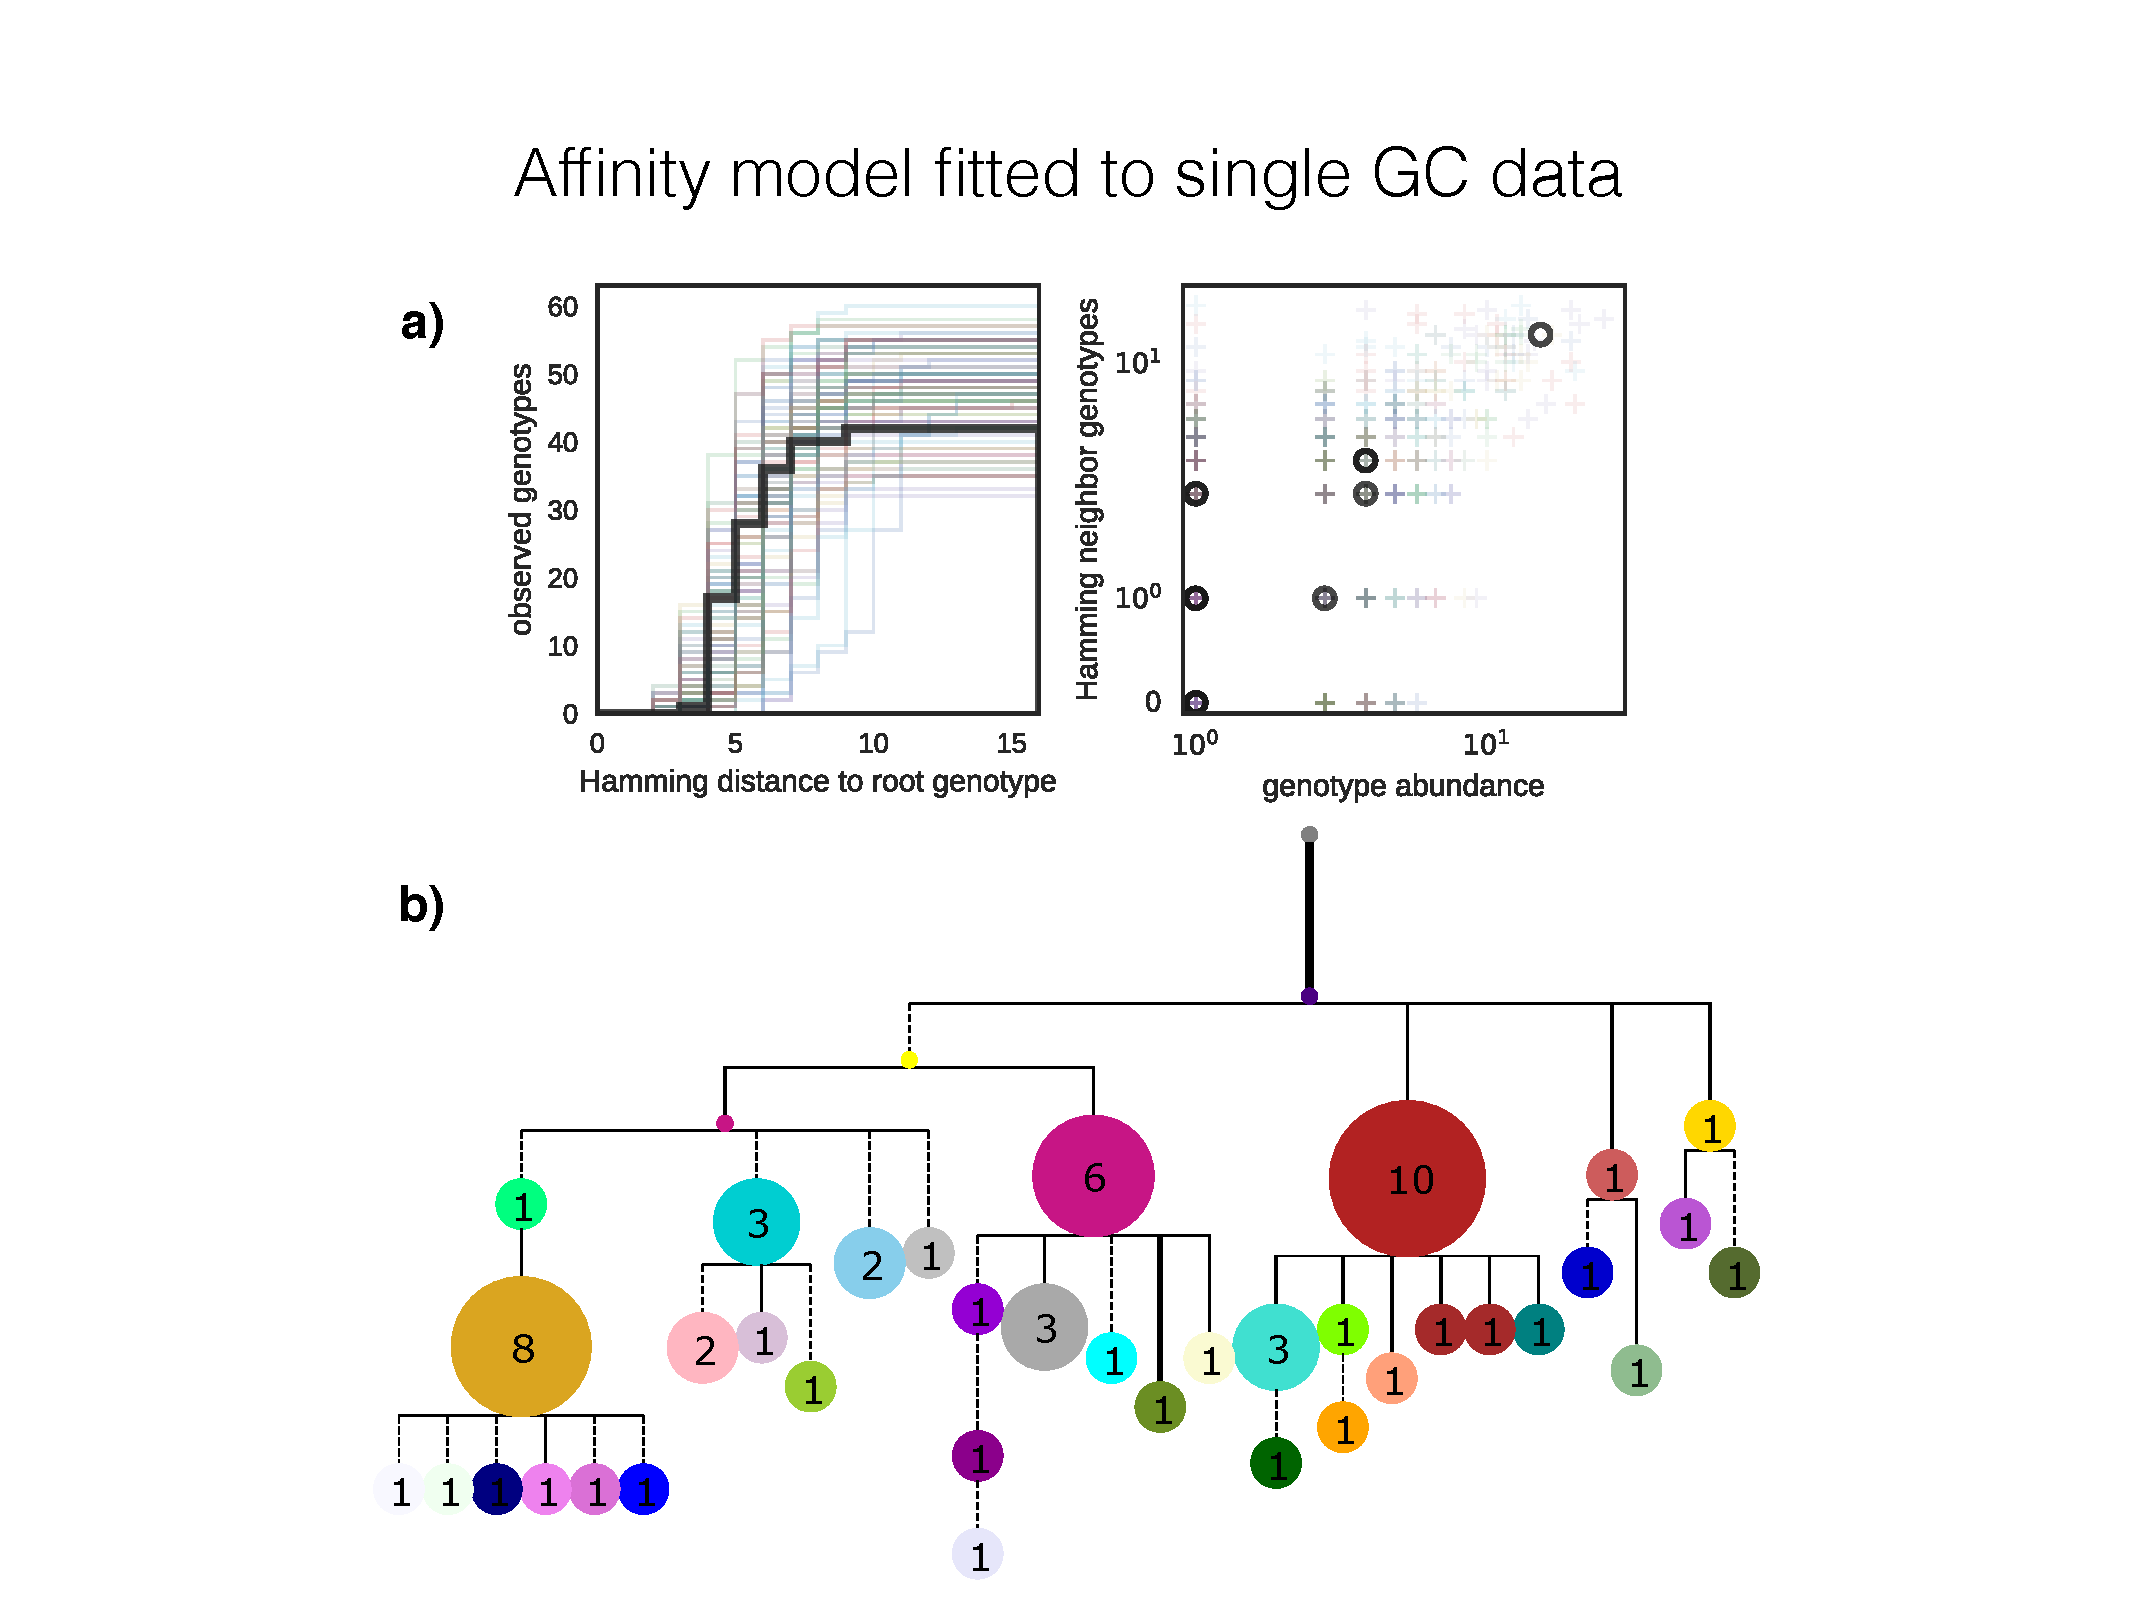
\includegraphics[width=0.8\textwidth]{figures/Tas-affsim_runstat.pdf}
    \caption{
        \label{fig:Tas-affsim_runstat}
        Affinity simulation with parameters fit to single cell data. In a) summary statistics of how well the simulations fit data (simulation in colors, data in black). In b) a typical tree topology from the simulation run.
    }
\end{figure}
\begin{figure}[!ht]
    \centering
    \includegraphics[width=0.8\textwidth]{figures/Tas-affsim_vali.pdf}
    \caption{
        \label{fig:Tas-affsim_vali}
        Performance of different inference method over the 100 simulations shown in \ref{fig:Tas-affsim_runstat}.
        Standard box plot format with the box covering the two middle quartiles (Q2=25\% to Q3=75\% percentile), whiskers extends these and extra 1.5 times the interquartile range and points outside this are plotted individually.
        The median is indicated by a black line.
        A rank of best to worst, is subjectively decided based on the metrics plotted and with importance of the metrics determined by the rank; COAR, MRCA, RF.
    }
\end{figure}

\begin{figure}[!ht]
    \centering
    \includegraphics[width=1\textwidth]{figures/Laura-affsim_runstat.pdf}
    \caption{
        \label{fig:Laura-affsim_runstat}
        Affinity simulation with parameters fit to HTS data. In a) summary statistics of how well the simulations fit data (simulations in grey shade, data in dark grey). In b) a typical tree topology from the simulation run.
    }
\end{figure}
\begin{figure}[!ht]
    \centering
    \includegraphics[width=0.8\textwidth]{figures/Laura-affsim_vali.pdf}
    \caption{
        \label{fig:Laura-affsim_vali}
        Performance of different inference method over the 100 simulations shown in \ref{fig:Laura-affsim_runstat}.
        Standard box plot format with the box covering the two middle quartiles (Q2=25\% to Q3=75\% percentile), whiskers extends these and extra 1.5 times the interquartile range and points outside this are plotted individually.
        The median is indicated by a black line.
        A rank of best to worst, is subjectively decided based on the metrics plotted and with importance of the metrics determined by the rank; COAR, MRCA.
    }
\end{figure}







%\fi
\chapter{Source code}
We find it unfortunate that the majority of previously published simulation methods does not offer publicly available software.
Therefore, to facilitate as much transparency and usability of the method presented in this work, we have chosen to share all our code as open source through a Git repository.
Hopefully this will encourage non developers to use and test our methods and potentially inspire to applications in fields that we have not yet investigated.

Methods for neutral, as well as affinity, simulations (used and described in chapter 3) are all collected in the same code repository along with SCons wrappers to run comparisons between inference methods (used in validation study in chapter 4).
This is all available in the \texttt{GCtree} code base:
\url{github.com/matsengrp/gctree}

In addition, the SCons commands used in the validation study, used to create the statistics in Appendix A and the figures in Appendix B, are listed below:
\begin{lstlisting}
scons --simulate --igphyml --gctree --dnaml --outdir=HTS_aff_sim --frame=1 --naive=CAGGTGCAGCTGGTGCAGTCTGGGGCTGAGGTGAAGAAGCCTGGGGCCTCAGTGAAGGTCTCCTGCAAGGCTTCTGGATACACCTTCACCGGCTACTATATGCACTGGGTGCGACAGGCCCCTGGACAAGGGCTTGAGTGGATGGGATGGATCAACCCTAACAGTGGTGGCACAAACTATGCACAGAAGTTTCAGGGCAGGGTCACCATGACCAGGGACACGTCCATCAGCACAGCCTACATGGAGCTGAGCAGGCTGAGATCTGACGACACGGCCGTGTATTACTGTGCGAGAGGGCCATTCCCGAATTACTATGGTACGGGGAGTTATTGGGGGGGTTTTGACTACTGGGGCCAGGGAACCCTGGTCACCGTCTCCTCA --experimental=<PATH TO FASTA FILE WITH EXPERIMENTAL GC SEQUENCES> --naiveIDexp=naive0 --lambda0=0.25 --selection --target_dist=10 --target_count=1000 --verbose --T=90 --carry_cap=10000 --skip_update=1000 --nsim=100 --n=150 --quick &> HTS_aff_sim.log

scons --simulate --igphyml --gctree --dnaml --outdir=HTS_neut_sim --frame=1 --nsim=100 --T=5 --lambda=2.5 --lambda0=3 --naive=CAGGTGCAGCTGGTGCAGTCTGGGGCTGAGGTGAAGAAGCCTGGGGCCTCAGTGAAGGTCTCCTGCAAGGCTTCTGGATACACCTTCACCGGCTACTATATGCACTGGGTGCGACAGGCCCCTGGACAAGGGCTTGAGTGGATGGGATGGATCAACCCTAACAGTGGTGGCACAAACTATGCACAGAAGTTTCAGGGCAGGGTCACCATGACCAGGGACACGTCCATCAGCACAGCCTACATGGAGCTGAGCAGGCTGAGATCTGACGACACGGCCGTGTATTACTGTGCGAGAGGGCCATTCCCGAATTACTATGGTACGGGGAGTTATTGGGGGGGTTTTGACTACTGGGGCCAGGGAACCCTGGTCACCGTCTCCTCA --experimental=<PATH TO FASTA FILE WITH EXPERIMENTAL GC SEQUENCES> --naiveIDexp=naive0 --quick &> HTS_neut_sim.log

scons --simulate --gctree --igphyml --dnaml --frame=1 --outdir=single_cell_aff_sim --naive=ggacctagcctcgtgaaaccttctcagactctgtccctcacctgttctgtcactggcgactccatcaccagtggttactggaactggatccggaaattcccagggaataaacttgagtacatggggtacataagctacagtggtagcacttactacaatccatctctcaaaagtcgaatctccatcactcgagacacatccaagaaccagtactacctgcagttgaattctgtgactactgaggacacagccacatattactgt --experimental=<PATH TO FASTA FILE WITH EXPERIMENTAL GC SEQUENCES> --naiveIDexp=naive0 --lambda0=0.25 --selection --target_dist=5 --target_count=100 --verbose --T=35 --nsim=100 --n=65 &> single_cell_aff_sim.log

scons --simulate --gctree --igphyml --dnaml --frame=1 --outdir=single_cell_neut_sim --nsim=100 --N=100 --n=70 --lambda=1.5 --lambda0=.25 --naive=ggacctagcctcgtgaaaccttctcagactctgtccctcacctgttctgtcactggcgactccatcaccagtggttactggaactggatccggaaattcccagggaataaacttgagtacatggggtacataagctacagtggtagcacttactacaatccatctctcaaaagtcgaatctccatcactcgagacacatccaagaaccagtactacctgcagttgaattctgtgactactgaggacacagccacatattactgt --experimental=<PATH TO FASTA FILE WITH EXPERIMENTAL GC SEQUENCES> --naiveIDexp=naive0 &> single_cell_neut_sim.log

\end{lstlisting}





\clearpage
\newpage
%% This defines the bibliography file (main.bib) and the bibliography style.
%% If you want to create a bibliography file by hand, change the contents of
%% this file to a `thebibliography' environment.  For more information 
%% see section 4.3 of the LaTeX manual.
\begin{singlespace}
\bibliography{main}
\bibliographystyle{plain}
\end{singlespace}

\end{document}

